% Options for packages loaded elsewhere
\PassOptionsToPackage{unicode}{hyperref}
\PassOptionsToPackage{hyphens}{url}
\PassOptionsToPackage{dvipsnames,svgnames,x11names}{xcolor}
%
\documentclass[
  letterpaper,
  DIV=11,
  numbers=noendperiod]{scrreprt}

\usepackage{amsmath,amssymb}
\usepackage{iftex}
\ifPDFTeX
  \usepackage[T1]{fontenc}
  \usepackage[utf8]{inputenc}
  \usepackage{textcomp} % provide euro and other symbols
\else % if luatex or xetex
  \usepackage{unicode-math}
  \defaultfontfeatures{Scale=MatchLowercase}
  \defaultfontfeatures[\rmfamily]{Ligatures=TeX,Scale=1}
\fi
\usepackage{lmodern}
\ifPDFTeX\else  
    % xetex/luatex font selection
\fi
% Use upquote if available, for straight quotes in verbatim environments
\IfFileExists{upquote.sty}{\usepackage{upquote}}{}
\IfFileExists{microtype.sty}{% use microtype if available
  \usepackage[]{microtype}
  \UseMicrotypeSet[protrusion]{basicmath} % disable protrusion for tt fonts
}{}
\makeatletter
\@ifundefined{KOMAClassName}{% if non-KOMA class
  \IfFileExists{parskip.sty}{%
    \usepackage{parskip}
  }{% else
    \setlength{\parindent}{0pt}
    \setlength{\parskip}{6pt plus 2pt minus 1pt}}
}{% if KOMA class
  \KOMAoptions{parskip=half}}
\makeatother
\usepackage{xcolor}
\usepackage{soul}
\setlength{\emergencystretch}{3em} % prevent overfull lines
\setcounter{secnumdepth}{5}
% Make \paragraph and \subparagraph free-standing
\ifx\paragraph\undefined\else
  \let\oldparagraph\paragraph
  \renewcommand{\paragraph}[1]{\oldparagraph{#1}\mbox{}}
\fi
\ifx\subparagraph\undefined\else
  \let\oldsubparagraph\subparagraph
  \renewcommand{\subparagraph}[1]{\oldsubparagraph{#1}\mbox{}}
\fi

\usepackage{color}
\usepackage{fancyvrb}
\newcommand{\VerbBar}{|}
\newcommand{\VERB}{\Verb[commandchars=\\\{\}]}
\DefineVerbatimEnvironment{Highlighting}{Verbatim}{commandchars=\\\{\}}
% Add ',fontsize=\small' for more characters per line
\usepackage{framed}
\definecolor{shadecolor}{RGB}{241,243,245}
\newenvironment{Shaded}{\begin{snugshade}}{\end{snugshade}}
\newcommand{\AlertTok}[1]{\textcolor[rgb]{0.68,0.00,0.00}{#1}}
\newcommand{\AnnotationTok}[1]{\textcolor[rgb]{0.37,0.37,0.37}{#1}}
\newcommand{\AttributeTok}[1]{\textcolor[rgb]{0.40,0.45,0.13}{#1}}
\newcommand{\BaseNTok}[1]{\textcolor[rgb]{0.68,0.00,0.00}{#1}}
\newcommand{\BuiltInTok}[1]{\textcolor[rgb]{0.00,0.23,0.31}{#1}}
\newcommand{\CharTok}[1]{\textcolor[rgb]{0.13,0.47,0.30}{#1}}
\newcommand{\CommentTok}[1]{\textcolor[rgb]{0.37,0.37,0.37}{#1}}
\newcommand{\CommentVarTok}[1]{\textcolor[rgb]{0.37,0.37,0.37}{\textit{#1}}}
\newcommand{\ConstantTok}[1]{\textcolor[rgb]{0.56,0.35,0.01}{#1}}
\newcommand{\ControlFlowTok}[1]{\textcolor[rgb]{0.00,0.23,0.31}{#1}}
\newcommand{\DataTypeTok}[1]{\textcolor[rgb]{0.68,0.00,0.00}{#1}}
\newcommand{\DecValTok}[1]{\textcolor[rgb]{0.68,0.00,0.00}{#1}}
\newcommand{\DocumentationTok}[1]{\textcolor[rgb]{0.37,0.37,0.37}{\textit{#1}}}
\newcommand{\ErrorTok}[1]{\textcolor[rgb]{0.68,0.00,0.00}{#1}}
\newcommand{\ExtensionTok}[1]{\textcolor[rgb]{0.00,0.23,0.31}{#1}}
\newcommand{\FloatTok}[1]{\textcolor[rgb]{0.68,0.00,0.00}{#1}}
\newcommand{\FunctionTok}[1]{\textcolor[rgb]{0.28,0.35,0.67}{#1}}
\newcommand{\ImportTok}[1]{\textcolor[rgb]{0.00,0.46,0.62}{#1}}
\newcommand{\InformationTok}[1]{\textcolor[rgb]{0.37,0.37,0.37}{#1}}
\newcommand{\KeywordTok}[1]{\textcolor[rgb]{0.00,0.23,0.31}{#1}}
\newcommand{\NormalTok}[1]{\textcolor[rgb]{0.00,0.23,0.31}{#1}}
\newcommand{\OperatorTok}[1]{\textcolor[rgb]{0.37,0.37,0.37}{#1}}
\newcommand{\OtherTok}[1]{\textcolor[rgb]{0.00,0.23,0.31}{#1}}
\newcommand{\PreprocessorTok}[1]{\textcolor[rgb]{0.68,0.00,0.00}{#1}}
\newcommand{\RegionMarkerTok}[1]{\textcolor[rgb]{0.00,0.23,0.31}{#1}}
\newcommand{\SpecialCharTok}[1]{\textcolor[rgb]{0.37,0.37,0.37}{#1}}
\newcommand{\SpecialStringTok}[1]{\textcolor[rgb]{0.13,0.47,0.30}{#1}}
\newcommand{\StringTok}[1]{\textcolor[rgb]{0.13,0.47,0.30}{#1}}
\newcommand{\VariableTok}[1]{\textcolor[rgb]{0.07,0.07,0.07}{#1}}
\newcommand{\VerbatimStringTok}[1]{\textcolor[rgb]{0.13,0.47,0.30}{#1}}
\newcommand{\WarningTok}[1]{\textcolor[rgb]{0.37,0.37,0.37}{\textit{#1}}}

\providecommand{\tightlist}{%
  \setlength{\itemsep}{0pt}\setlength{\parskip}{0pt}}\usepackage{longtable,booktabs,array}
\usepackage{calc} % for calculating minipage widths
% Correct order of tables after \paragraph or \subparagraph
\usepackage{etoolbox}
\makeatletter
\patchcmd\longtable{\par}{\if@noskipsec\mbox{}\fi\par}{}{}
\makeatother
% Allow footnotes in longtable head/foot
\IfFileExists{footnotehyper.sty}{\usepackage{footnotehyper}}{\usepackage{footnote}}
\makesavenoteenv{longtable}
\usepackage{graphicx}
\makeatletter
\def\maxwidth{\ifdim\Gin@nat@width>\linewidth\linewidth\else\Gin@nat@width\fi}
\def\maxheight{\ifdim\Gin@nat@height>\textheight\textheight\else\Gin@nat@height\fi}
\makeatother
% Scale images if necessary, so that they will not overflow the page
% margins by default, and it is still possible to overwrite the defaults
% using explicit options in \includegraphics[width, height, ...]{}
\setkeys{Gin}{width=\maxwidth,height=\maxheight,keepaspectratio}
% Set default figure placement to htbp
\makeatletter
\def\fps@figure{htbp}
\makeatother

\usepackage{float}
\usepackage{tabularray}
\usepackage[normalem]{ulem}
\usepackage{graphicx}
\usepackage{rotating}
\UseTblrLibrary{siunitx}
\NewTableCommand{\tinytableDefineColor}[3]{\definecolor{#1}{#2}{#3}}
\newcommand{\tinytableTabularrayUnderline}[1]{\underline{#1}}
\newcommand{\tinytableTabularrayStrikeout}[1]{\sout{#1}}
\usepackage{amsfonts}
\usepackage{amsmath}
\usepackage{mdframed}
\usepackage{lipsum}
\usepackage{tcolorbox}
\usepackage{xcolor}
\usepackage[thickspace,nobracket]{actuarialangle}
\usepackage{tikz}
\usetikzlibrary{shapes.geometric,arrows.meta,positioning,calc}
\KOMAoption{captions}{tableheading}
\makeatletter
\@ifpackageloaded{tcolorbox}{}{\usepackage[skins,breakable]{tcolorbox}}
\@ifpackageloaded{fontawesome5}{}{\usepackage{fontawesome5}}
\definecolor{quarto-callout-color}{HTML}{909090}
\definecolor{quarto-callout-note-color}{HTML}{0758E5}
\definecolor{quarto-callout-important-color}{HTML}{CC1914}
\definecolor{quarto-callout-warning-color}{HTML}{EB9113}
\definecolor{quarto-callout-tip-color}{HTML}{00A047}
\definecolor{quarto-callout-caution-color}{HTML}{FC5300}
\definecolor{quarto-callout-color-frame}{HTML}{acacac}
\definecolor{quarto-callout-note-color-frame}{HTML}{4582ec}
\definecolor{quarto-callout-important-color-frame}{HTML}{d9534f}
\definecolor{quarto-callout-warning-color-frame}{HTML}{f0ad4e}
\definecolor{quarto-callout-tip-color-frame}{HTML}{02b875}
\definecolor{quarto-callout-caution-color-frame}{HTML}{fd7e14}
\makeatother
\makeatletter
\makeatother
\makeatletter
\@ifpackageloaded{bookmark}{}{\usepackage{bookmark}}
\makeatother
\makeatletter
\@ifpackageloaded{caption}{}{\usepackage{caption}}
\AtBeginDocument{%
\ifdefined\contentsname
  \renewcommand*\contentsname{Table of contents}
\else
  \newcommand\contentsname{Table of contents}
\fi
\ifdefined\listfigurename
  \renewcommand*\listfigurename{List of Figures}
\else
  \newcommand\listfigurename{List of Figures}
\fi
\ifdefined\listtablename
  \renewcommand*\listtablename{List of Tables}
\else
  \newcommand\listtablename{List of Tables}
\fi
\ifdefined\figurename
  \renewcommand*\figurename{Figure}
\else
  \newcommand\figurename{Figure}
\fi
\ifdefined\tablename
  \renewcommand*\tablename{Table}
\else
  \newcommand\tablename{Table}
\fi
}
\@ifpackageloaded{float}{}{\usepackage{float}}
\floatstyle{ruled}
\@ifundefined{c@chapter}{\newfloat{codelisting}{h}{lop}}{\newfloat{codelisting}{h}{lop}[chapter]}
\floatname{codelisting}{Listing}
\newcommand*\listoflistings{\listof{codelisting}{List of Listings}}
\makeatother
\makeatletter
\@ifpackageloaded{caption}{}{\usepackage{caption}}
\@ifpackageloaded{subcaption}{}{\usepackage{subcaption}}
\makeatother
\makeatletter
\@ifpackageloaded{tcolorbox}{}{\usepackage[skins,breakable]{tcolorbox}}
\makeatother
\makeatletter
\@ifundefined{shadecolor}{\definecolor{shadecolor}{rgb}{.97, .97, .97}}
\makeatother
\makeatletter
\makeatother
\makeatletter
\makeatother
\ifLuaTeX
  \usepackage{selnolig}  % disable illegal ligatures
\fi
\IfFileExists{bookmark.sty}{\usepackage{bookmark}}{\usepackage{hyperref}}
\IfFileExists{xurl.sty}{\usepackage{xurl}}{} % add URL line breaks if available
\urlstyle{same} % disable monospaced font for URLs
\hypersetup{
  pdftitle={BIOS 526 Modern Regression Analysis},
  pdfauthor={Emily Peterson},
  colorlinks=true,
  linkcolor={blue},
  filecolor={Maroon},
  citecolor={Blue},
  urlcolor={Blue},
  pdfcreator={LaTeX via pandoc}}

\title{BIOS 526 Modern Regression Analysis}
\author{Emily Peterson}
\date{2025-01-01}

\begin{document}
\maketitle
\ifdefined\Shaded\renewenvironment{Shaded}{\begin{tcolorbox}[breakable, boxrule=0pt, sharp corners, borderline west={3pt}{0pt}{shadecolor}, interior hidden, enhanced, frame hidden]}{\end{tcolorbox}}\fi

\renewcommand*\contentsname{Table of contents}
{
\hypersetup{linkcolor=}
\setcounter{tocdepth}{2}
\tableofcontents
}
\bookmarksetup{startatroot}

\hypertarget{introduction}{%
\chapter*{Introduction}\label{introduction}}
\addcontentsline{toc}{chapter}{Introduction}

\markboth{Introduction}{Introduction}

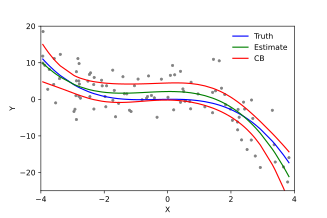
\includegraphics[width=5.22917in,height=\textheight]{fig/intro.png}

Welcome to Modern Regression!

\textbf{Course Number:} 526 \textbf{Section Number:} 1

\textbf{Credit Hours:} 3 \textbf{Semester:} Fall 2026

\textbf{Class Hours and Location:} Monday \& Wednesday 1:30-2:50pm at
CNR 1051

\textbf{Instructor Name: Emily Peterson (Emily)}
emily.nancy.peterson@emory.edu

\textbf{Teaching Assistants:} Winn Wu
\href{mailto:winn.wu@emory.edu}{wencheng.wu@emory.edu} Office hours:
Tuesdays 10Am-12PM email to request remote session
~\url{https://emory.zoom.us/j/3226912694}.~. Location GCR 3rd floor
library.

\textbf{Course Description:} This course introduces students to modern
regression techniques commonly used in analyzing public health data.
Specific topics include: (1) methods for modeling longitudinal and
multi-level data that account for within group correlation (e.g.,
mixed-effect models, generalized estimating equations); (2) modeling
non-linear relationships using splines and generalized additive models;
and (3) shrinkage methods and bias-variance tradeoffs.

This course draws motivating examples from environmental and social
epidemiology, health services research, clinical studies, etc. The
course provides a survey of advanced regression approaches with a focus
on data analysis and interpretation. Students will gain an understanding
of methods that will facilitate future independent and collaborative
research for modern research problems. Students will gain practical
experiences using the R language for statistical computing.

This is a required course for MSPH students in BIOS in the fall of their
second year. It is also an elective course for PhD BIOS students in
their second year interested in advanced modeling techniques.

\textbf{Pre-reqs:} BIOS 509 and BIOS 513 or equivalent. Students are
assumed to have background knowledge in linear algebra and multivariate
calculus. Experience with R (BIOS 545).

\textbf{Using this book:} This book consists of the lectures notes used
for this course in modern regression techniques. We will use this book
to review concepts in class. The book is split into separate modules
covering the particular topics in this course. In-class activities and
homework assignments are outlined for each module.

\begin{tcolorbox}[enhanced jigsaw, breakable, colbacktitle=quarto-callout-warning-color!10!white, left=2mm, colframe=quarto-callout-warning-color-frame, opacityback=0, coltitle=black, colback=white, rightrule=.15mm, title={Warning}, titlerule=0mm, opacitybacktitle=0.6, leftrule=.75mm, toprule=.15mm, arc=.35mm, bottomtitle=1mm, toptitle=1mm, bottomrule=.15mm]

I am frequently editing notes in this book. I do not suggest reading
ahead in future modules as I may change material or assignments during
the semester.

\end{tcolorbox}

\begin{center}\rule{0.5\linewidth}{0.5pt}\end{center}

\bookmarksetup{startatroot}

\hypertarget{module-0-multiple-linear-regression-review}{%
\chapter*{Module 0: Multiple Linear Regression
Review}\label{module-0-multiple-linear-regression-review}}
\addcontentsline{toc}{chapter}{Module 0: Multiple Linear Regression
Review}

\markboth{Module 0: Multiple Linear Regression Review}{Module 0:
Multiple Linear Regression Review}

\begin{verbatim}
Warning: package 'dplyr' was built under R version 4.4.3
\end{verbatim}

\textbf{Readings}

\begin{itemize}
\tightlist
\item
  Review matrix algebra
  \href{https://www.math.uwaterloo.ca/~hwolkowi/matrixcookbook.pdf}{Matrix
  Cookbook}.
\item
  BIOS 509 notes on Applied Linear Regression.\\
\item
  Gelman \& Hill-style regression intuition (figure referenced in
  class).
\end{itemize}

\textbf{Overview \& Concepts:} In this module you will get a brief
review of concepts learned in BIOS 509 including the multiple linear
regression (MLR) framework for \textbf{estimation, interpretation,
prediction, and diagnostics}. This material will not be included in the
labs or quizzes, but is simply a review guide for you to brush up on
material needed for Modules 1-3.

\begin{itemize}
\item
  Linear regression model in matrix notation
\item
  Inference for regression coefficient estimates, expected values, and
  predictions.
\item
  Dummy variables
\item
  Effect modification and confounding
\end{itemize}

\begin{center}\rule{0.5\linewidth}{0.5pt}\end{center}

\hypertarget{motivation-and-examples}{%
\subsection*{Motivation and Examples}\label{motivation-and-examples}}
\addcontentsline{toc}{subsection}{Motivation and Examples}

\begin{tcolorbox}[enhanced jigsaw, breakable, colbacktitle=quarto-callout-important-color!10!white, left=2mm, colframe=quarto-callout-important-color-frame, opacityback=0, coltitle=black, colback=white, rightrule=.15mm, title=\textcolor{quarto-callout-important-color}{\faExclamation}\hspace{0.5em}{Important}, titlerule=0mm, opacitybacktitle=0.6, leftrule=.75mm, toprule=.15mm, arc=.35mm, bottomtitle=1mm, toptitle=1mm, bottomrule=.15mm]

\textbf{Multiple Linear Regression (MLR)} is the standard extension of
simple linear regression to include two or more predictors.

Formally:

\[
y_i = \beta_0 + \beta_1 x_{i1} + \cdots + \beta_p x_{ip} + \epsilon_i,
\quad \epsilon_i \sim N(0,\sigma^2)
\]

\(y_i\) = outcome (continuous response)

\(x_{ij}\) = predictor variables (continuous or categorical)

\(\beta_j\) = regression coefficients (effects of predictors, holding
others constant)

\(\epsilon_i\) = error term

\textbf{Matrix form}

\[
\mathbf{y} = \mathbf{X}\boldsymbol{\beta} + \boldsymbol{\epsilon}, 
\quad \mathbb{E}[\boldsymbol{\epsilon}] = \mathbf{0}, 
\quad \operatorname{Var}(\boldsymbol{\epsilon}) = \sigma^2 \mathbf{I}
\]

\textbf{Key points about MLR:}

\begin{itemize}
\item
  Goal: quantify how multiple predictors are simultaneously associated
  with an outcome.
\item
  Interpretation: each \(\beta_j\) is the average change in \(y\) for a
  one-unit change in \(x_{j}\), holding other predictors fixed.
\item
  Uses: adjust for confounding, test effect modification (interactions),
  improve prediction accuracy.
\item
  Assumptions: linearity, independence, constant variance
  (homoscedasticity), and normally distributed errors.
\end{itemize}

In short: MLR models a continuous outcome as a linear combination of
multiple explanatory variables, enabling adjusted and interpretable
population-level associations.

\end{tcolorbox}

\textbf{Motivating Example:(NLSY):} maternal traits vs.~child cognitive
score (age 3).

We want to answer the question: \textbf{What maternal traits are
associated with a child's cognitive score at age 3?}

Variables:

\begin{itemize}
\tightlist
\item
  \texttt{score}: cognitive test score (outcome)
\item
  \texttt{age}: maternal age at delivery (numeric)
\item
  \texttt{edu}: maternal education --- 1: \textless HS, 2: HS, 3: some
  college, 4: college+
\end{itemize}

\textbf{Model (baseline):}

\[y_i = \beta_0 + \beta_1 \text{age}_i + \epsilon_i\]

\textbf{MLR (with confounding):}

\[
y_i = \beta_0 + \beta_1\text{age}_i + \beta_2\mathbb{1}(\text{edu}=2) + \beta_3\mathbb{1}(\text{edu}=3) + \beta_4\mathbb{1}(\text{edu}=4) + \epsilon_i
\]

Below we give some quick visuals

\begin{verbatim}
Rows: 400
Columns: 3
$ score <dbl> 120, 89, 78, 42, 115, 97, 94, 68, 103, 94, 117, 64, 72, 104, 78,~
$ edu   <dbl> 2, 1, 2, 1, 4, 1, 1, 2, 3, 3, 2, 4, 2, 2, 3, 1, 1, 3, 3, 2, 2, 2~
$ age   <dbl> 21, 17, 19, 20, 26, 20, 20, 24, 19, 24, 24, 29, 19, 23, 26, 22, ~
\end{verbatim}


\includegraphics{Module_0_MLR_files/figure-pdf/unnamed-chunk-2-1.pdf}

\begin{center}\rule{0.5\linewidth}{0.5pt}\end{center}

\hypertarget{simple-linear-regression}{%
\section*{\texorpdfstring{\ul{Simple Linear
Regression}}{Simple Linear Regression}}\label{simple-linear-regression}}
\addcontentsline{toc}{section}{\ul{Simple Linear Regression}}

\markright{\ul{Simple Linear Regression}}

Linear regression is a method that summarizes how the average values of
a numerical outcome variable vary over subpopulations (covariate values)
defined by linear functions of predictors. Two goals of linear
regression:

\begin{enumerate}
\def\labelenumi{\arabic{enumi}.}
\item
  \emph{Prediction of outcome values given fixed predictor values.}
\item
  \emph{Assessment of impact of predictors on the outcome (Estimation).}
\end{enumerate}

Let \(y_i\) denote the test score for a given child \(i\). \(age_i\)
denotes the corresponding maternal age at delivery for mom \(i\)
corresponding to child \(i\), and \(\epsilon_i\) denotes the error term.
We will consider the following linear model:

\begin{equation}\protect\hypertarget{eq-one}{}{y_i = \beta_0 + \beta_1 \cdot age_i + \epsilon_i, \quad i = 1,2,3,...,400}\label{eq-one}\end{equation}

We can write Eq. 1 in matrix form by stacking observations by row:

\[\begin{align}
\mathbf{Y}& = \begin{bmatrix} y_1 \\ y_2\\ \vdots \\ y_n \end{bmatrix} = 
\begin{bmatrix}
\beta_0 + \beta_1 x_1\\ \beta_0 + \beta_1 x_2 \\ \vdots \\ \beta_0 + \beta_1 x_n \end{bmatrix} + \begin{bmatrix} \epsilon_1 \\ \epsilon_2 \\  \vdots \\ \epsilon_n \end{bmatrix}\\
& = \begin{bmatrix} 1 & x_1\\1 & x_2\\ \vdots \\ 1 & x_n\end{bmatrix} \begin{bmatrix}\beta_0 \\ \beta_1\end{bmatrix} + \begin{bmatrix} \epsilon_1 \\ \epsilon_2 \\  \vdots \\ \epsilon_n \end{bmatrix}\\
&= \mathbf{X\beta + \epsilon}
\end{align}\]

Clearly, we cannot find \(\mathbf{\beta}\) such that this model fits all
of our data perfectly.

\textbf{Model Assumptions:}

\begin{itemize}
\item
  \(y_i\) is a linear function of \(age_i\), i.e,
  \(E(\mathbf{Y}) = \mathbf{X\beta} = \mathbf{Age\beta}\) is linear in
  the \(\beta's\).
\item
  \(\beta_0=\) the test score for a child born of a mother at age=0 (not
  meaningful!)
\item
  \(\beta_1=\) average increase in test score associated with one year
  increase in maternal age.
\item
  \(E(\epsilon_i) = 0\) {[}Expectation of the errors is zero{]}.
\end{itemize}

\begin{center}\rule{0.5\linewidth}{0.5pt}\end{center}

\hypertarget{least-squares-solution}{%
\subsubsection*{\texorpdfstring{\ul{Least Squares
Solution}}{Least Squares Solution}}\label{least-squares-solution}}
\addcontentsline{toc}{subsubsection}{\ul{Least Squares Solution}}

\textbf{Our aim is to find estimates of} \(\beta_0\) \textbf{and}
\(\beta_1\) \textbf{that ``best'' fit the data, but what does ``best''
mean?}

We seek \((\hat{\beta}_0, \hat{\beta}_1)\) that minimizes a
extcolor\{red\}\{loss function\}.

Our approach is to minimize the sum of extcolor\{red\}\{squared
differences\} between \(\mathbf{Y}\) and
\(\hat{Y} = \mathbf{X\hat{\beta}}\), i.e., this defines the differences
between \(\mathbf{Y}\) and the predicted value \(\hat{Y}\) based on a
fixed set of \(\beta's\).

\begin{tcolorbox}[enhanced jigsaw, rightrule=.15mm, breakable, left=2mm, colframe=quarto-callout-note-color-frame, opacityback=0, leftrule=.75mm, toprule=.15mm, colback=white, arc=.35mm, bottomrule=.15mm]

\textbf{Theorem}\vspace{2mm}

If \(\mathbf{Y} = \mathbf{X\beta} + \mathbf{\epsilon}\) then the value
of \(\hat{\beta}\) that minimizes
\((\mathbf{Y - \hat{Y}})^T(\mathbf{Y - \hat{Y}})\) is
\(\hat{\beta} = (X'X)^{-1} X'y\).

\begin{itemize}
\item
  \(\mathbf{\hat{Y}} = \mathbf{X \hat{\beta}}\) is the fitted
  (predicted) value.
\item
  \(\mathbf{\hat{\epsilon}} = \mathbf{Y} - \mathbf{X\hat{\beta}}\)
  defines the residual error.
\end{itemize}

\end{tcolorbox}

\begin{tcolorbox}[enhanced jigsaw, rightrule=.15mm, breakable, left=2mm, colframe=quarto-callout-tip-color-frame, opacityback=0, leftrule=.75mm, toprule=.15mm, colback=white, arc=.35mm, bottomrule=.15mm]

\textbf{Derivation (matrix calculus)}\vspace{2mm}

We estimate \(\hat\beta\) by minimizing the \textbf{residual sum of
squares} (RSS):

\[
\hat\beta = argmin_{\beta}\; S(\beta),
\qquad
S(\beta)=|\mathbf{y}-\mathbf{X}\beta|_2^2
=(\mathbf{y}-\mathbf{X}\beta)^\top(\mathbf{y}-\mathbf{X}\beta).
\]

\textbf{Expand the residual quadratic:} \[
\begin{aligned}
S(\beta)
&= \mathbf{y}^\top\mathbf{y}
 - 2\,\beta^\top\mathbf{X}^\top\mathbf{y}
 + \beta^\top\mathbf{X}^\top\mathbf{X}\,\beta.
\end{aligned}
\]

\textbf{Differentiate and set to zero (normal equations):} \[
\nabla_\beta S(\beta)
= -2\,\mathbf{X}^\top\mathbf{y}
 + 2\,\mathbf{X}^\top\mathbf{X}\,\beta
= \mathbf{0}
\quad\Longrightarrow\quad
\mathbf{X}^\top\mathbf{X}\,\hat\beta
= \mathbf{X}^\top\mathbf{y}.
\]

\textbf{Solution (full column rank} \(\mathbf{X}\): \[
\hat\beta_{OLS}
= (\mathbf{X}^\top\mathbf{X})^{-1}\mathbf{X}^\top\mathbf{y}.
\] For OLS, we have a nice closed-form solution.

Other loss functions or models often require iterative optimization
routines.

\textbf{Fitted values \& projection:} \[
 \hat{\mathbf{y}}=\mathbf{X}\hat\beta
= \underbrace{\mathbf{X}(\mathbf{X}^\top\mathbf{X})^{-1}\mathbf{X}^\top}_{\mathbf{H}}\mathbf{y},
\quad
\text{with }\mathbf{H}^\top=\mathbf{H},\;\mathbf{H}^2=\mathbf{H},\;\operatorname{tr}(\mathbf{H})=p \text{ (number of predictors)}.
\]

\textbf{Orthogonality of residuals: We assume independence between
covariate values and residuals.} \[
\mathbf{r}=\mathbf{y}-\hat{\mathbf{y}},\qquad
\mathbf{X}^\top\mathbf{r}=\mathbf{0}.
\]

\end{tcolorbox}

\hypertarget{geometric-interpretation-of-the-ols-estimate}{%
\subsubsection*{Geometric Interpretation of the OLS
estimate}\label{geometric-interpretation-of-the-ols-estimate}}
\addcontentsline{toc}{subsubsection}{Geometric Interpretation of the OLS
estimate}

The fitted values \(\hat{y}\) are a linear transformation of \(y\). We
see from the figure \(y\) in real space is projected on \(\hat{y}\) in
model space.

\begin{itemize}
\item
  The \ul{HAT} \ul{matrix} is defined as
  \(\mathbf{H} = \mathbf{X(X^{T} X)^{-1}X^T}\). It is a projection
  matrix that projects \(y\) \(\rightarrow\) \(\hat{y}\).

  \[
  \begin{align}
  \mathbf{\hat{y}} &= \mathbf{X\hat{\beta}}\\
  &= \mathbf{X(X'X)^{-1}X'y}
  \end{align}
  \]
\item
  The projection matrix is idempotent, i.e., \(HH=H\).
\item
  The trace \(=\) rank of \(X\) or the number of covariates plus
  intercept, i.e, \(tr(H) = p\).
\item
  \(\hat{\mathbf{Y}}\) and \(\mathbf{\hat{\epsilon}}\) are independent,
  i.e., orthogonal (perpendicular in model space).
\end{itemize}

\begin{figure}

{\centering 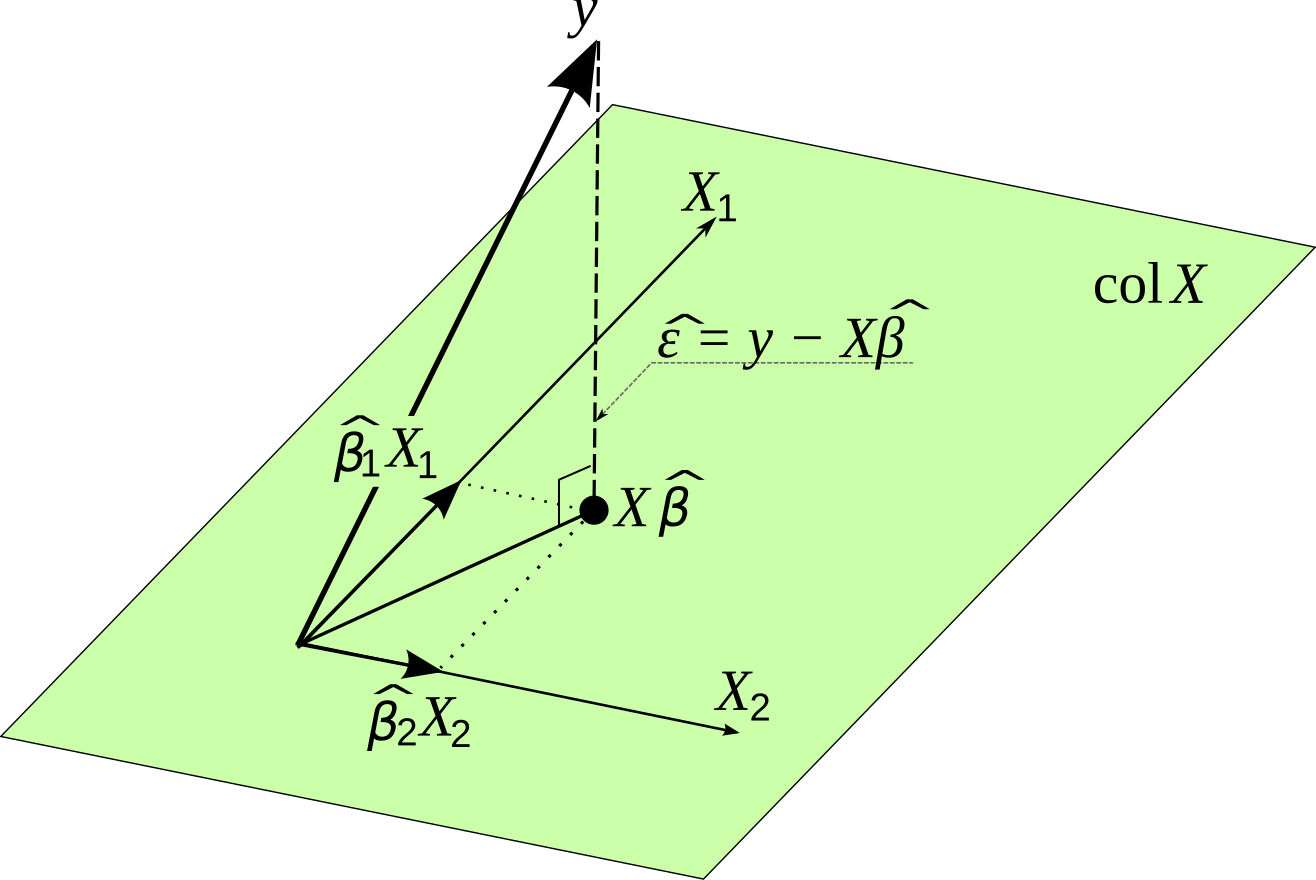
\includegraphics{fig/OLSgeo2.png}

}

\caption{A geometrical interpretation of least squares.}

\end{figure}

\begin{center}\rule{0.5\linewidth}{0.5pt}\end{center}

\hypertarget{properties-of-the-ols-estimator-hatbeta}{%
\subsubsection*{\texorpdfstring{\ul{Properties of the OLS Estimator
\(\hat{\beta}\)}}{Properties of the OLS Estimator \textbackslash hat\{\textbackslash beta\}}}\label{properties-of-the-ols-estimator-hatbeta}}
\addcontentsline{toc}{subsubsection}{\ul{Properties of the OLS Estimator
\(\hat{\beta}\)}}

\begin{enumerate}
\def\labelenumi{\arabic{enumi}.}
\tightlist
\item
  If \(E(Y) = X\beta\) then \(\hat{\beta}\) is unbiased for \(\beta\).
\end{enumerate}

\[
\begin{align}
E(\hat{\beta}) & = E[(X^TX)^{-1} X^Ty]\\
& = (X^T X)^{-1} X^T E(y)\\
& =(X^T X)^{-1} X^T X \beta\\
& = \beta
\end{align}
\]

\begin{enumerate}
\def\labelenumi{\arabic{enumi}.}
\setcounter{enumi}{1}
\item
  \(\hat{\beta}\) is consistent estimation of \(\beta\) under very
  general assumptions, i.e.,
  \(lim_{n\rightarrow \infty} P(|\hat{\beta} - \beta|>\epsilon) = 0\).
\item
  \(\mathbf{\hat{Y}}\) is an unbiased estimator of the mean trend
  \(\mathbf{X\beta}\).
\item
  If \(cov(y) = \sigma^2 I\), the covariance of the estimator
  \(cov(\mathbf{\hat{\beta}}) = \sigma^2 (X'X)^{-1}\).
\end{enumerate}

\textbf{Find the} \(\operatorname{Cov}(\hat{\beta})\)

We have the linear model \[
\mathbf{y} = \mathbf{X}\beta + \boldsymbol{\epsilon}, 
\qquad \mathbb{E}[\boldsymbol{\epsilon}] = \mathbf{0}, 
\qquad \operatorname{Var}(\boldsymbol{\epsilon}) = \sigma^2 \mathbf{I}.
\]

The OLS estimator is \[
\hat{\beta} = (\mathbf{X}^\top \mathbf{X})^{-1}\mathbf{X}^\top \mathbf{y}
= \beta + (\mathbf{X}^\top \mathbf{X})^{-1}\mathbf{X}^\top \boldsymbol{\epsilon}.
\]

Therefore,

\[
\begin{aligned}
\operatorname{Cov}(\hat{\beta})
&= \operatorname{Var}\!\left[(\mathbf{X}^\top \mathbf{X})^{-1}\mathbf{X}^\top \boldsymbol{\epsilon}\right] \\
&= (\mathbf{X}^\top \mathbf{X})^{-1}\mathbf{X}^\top 
      \underbrace{\operatorname{Var}(\boldsymbol{\epsilon})}_{\sigma^2 \mathbf{I}}
      \mathbf{X}(\mathbf{X}^\top \mathbf{X})^{-1} \\
&= \sigma^2 \, (\mathbf{X}^\top \mathbf{X})^{-1}.
\end{aligned}
\]

\begin{tcolorbox}[enhanced jigsaw, rightrule=.15mm, breakable, left=2mm, colframe=quarto-callout-note-color-frame, opacityback=0, leftrule=.75mm, toprule=.15mm, colback=white, arc=.35mm, bottomrule=.15mm]

\textbf{Gauss-Markov Theorem:}\vspace{2mm}

The Gauss-Markov Theorem states that, under the classical linear
regression assumptions, the OLS estimator is the \textbf{Best Linear
Unbiased Estimator (BLUE)} of the coefficients---that is, it has the
lowest variance among all linear and unbiased estimators.

\begin{itemize}
\item
  \(\mathbf{Y} = \mathbf{X\beta} +\epsilon\)
\item
  \(E(\epsilon) = 0\) and \(cov(\epsilon) = \sigma^2 I\)
\item
  \(var(\hat{\beta}) = \sigma^2 (X'X)^{-1}\)
\item
  \(\hat{\beta}\) is the best (minimum variance) unbiased estimator
  (BLUE) for \(\mathbf{\beta}\).
\end{itemize}

\end{tcolorbox}

\begin{center}\rule{0.5\linewidth}{0.5pt}\end{center}

\hypertarget{ols-calculation-in-r}{%
\section*{OLS Calculation in R}\label{ols-calculation-in-r}}
\addcontentsline{toc}{section}{OLS Calculation in R}

\markright{OLS Calculation in R}

\begin{Shaded}
\begin{Highlighting}[]
\CommentTok{\#Calculate beta manually}
\NormalTok{X }\OtherTok{=} \FunctionTok{cbind}\NormalTok{(}\DecValTok{1}\NormalTok{, dat}\SpecialCharTok{$}\NormalTok{age) }\CommentTok{\#Design Matrix}
\NormalTok{Y }\OtherTok{=}\NormalTok{ dat}\SpecialCharTok{$}\NormalTok{score }\CommentTok{\#Response/Outcome Vector}
\NormalTok{beta }\OtherTok{=} \FunctionTok{solve}\NormalTok{( }\FunctionTok{t}\NormalTok{(X) }\SpecialCharTok{\%*\%}\NormalTok{ X) }\SpecialCharTok{\%*\%} \FunctionTok{t}\NormalTok{(X) }\SpecialCharTok{\%*\%}\NormalTok{ Y}
\NormalTok{beta}
\end{Highlighting}
\end{Shaded}

\begin{verbatim}
           [,1]
[1,] 67.7826813
[2,]  0.8402729
\end{verbatim}

\begin{Shaded}
\begin{Highlighting}[]
\CommentTok{\#Visualize the univariate association}
\FunctionTok{plot}\NormalTok{(score }\SpecialCharTok{\textasciitilde{}}\NormalTok{ age, }\AttributeTok{data =}\NormalTok{ dat, }\AttributeTok{xlab =} \StringTok{"Age"}\NormalTok{, }\AttributeTok{ylab =} \StringTok{"Score"}\NormalTok{)}
\FunctionTok{abline}\NormalTok{(beta, }\AttributeTok{lwd =} \DecValTok{3}\NormalTok{, }\AttributeTok{col =} \DecValTok{2}\NormalTok{)}
\end{Highlighting}
\end{Shaded}

\begin{figure}[H]

{\centering 
\includegraphics{Module_0_MLR_files/figure-pdf/unnamed-chunk-3-1.pdf}

}

\end{figure}

We see that the regression coefficient estimate for age is \(0.840\).
This means that for every 0.840 unit increase in \(age\), there is a
1-unit increase in \(child score\).

\begin{center}\rule{0.5\linewidth}{0.5pt}\end{center}

\hypertarget{statistical-linear-regression-inference}{%
\section*{\texorpdfstring{\ul{Statistical Linear Regression \&
Inference}}{Statistical Linear Regression \& Inference}}\label{statistical-linear-regression-inference}}
\addcontentsline{toc}{section}{\ul{Statistical Linear Regression \&
Inference}}

\markright{\ul{Statistical Linear Regression \& Inference}}

{The relation between OLS, Normality, and Maximum Likelihood}

So far, we have not discussed the distribution of the errors. For OLS we
\textbf{did not need} to make any distributional assumption.

\[
\hat{\beta}_{OLS} = (X^TX)^{-1}X^Ty
\]

But for inference (SEs, CIs, p-values), we need to make some
distributional assumptions for the errors. Let's now assume\ldots{}

\[
y_i = \beta_0 + \beta_1 age_i + \epsilon_i, \quad i=1, ..., 400
\] where \(\epsilon \overset{iid}{\sim} N(0, \sigma^2)\).

What does i.i.d mean? \ul{identically and independently distributed.}
This implies the following model:

\begin{itemize}
\item
  \(y_i\) is normally distributed.
\item
  This parametrization is equal to

  \[y_i \sim N(\beta_0 + \beta_1 x_i,\sigma^2)\].
\item
  where \(\beta_0 + \beta_1 x_i\) captures the trend
\item
  where \(\sigma^2\) captures the variability (uncertainty) around the
  trend. It is constant, i.e., the same across all observations.
\item
  \textbf{In matrix form:}
  \(\mathbf{Y} \sim N(\mathbf{X\beta}, \Sigma)\) where
  \(\Sigma = \sigma^2I\).
\item
  \(\sigma^2\) is unknown!
\end{itemize}

\begin{center}\rule{0.5\linewidth}{0.5pt}\end{center}

\hypertarget{the-maximum-likelihood}{%
\subsubsection*{\texorpdfstring{\ul{The Maximum
Likelihood}}{The Maximum Likelihood}}\label{the-maximum-likelihood}}
\addcontentsline{toc}{subsubsection}{\ul{The Maximum Likelihood}}

The likelihood of the normal distribution is given by

\[
L(\beta, \sigma^2, y) = (2\pi \sigma^2)^{-n/2} exp\left(\frac{-1}{2\sigma^2} (Y-X\beta)'(Y-X\beta)\right)
\]

Taking the log of the likelihood, we get:

\[
l(\beta, \sigma^2, y) = \frac{-n}{2} log(2\pi\sigma^2) - \frac{1}{2\sigma^2} (Y-X\beta)'(Y-X\beta)
\]

To find \textbf{Maximum Likelihood Estimators} we take partial
derivatives and set the equal to zero to find the estimators that
maximize the log-likelihood.

What do we get?

\begin{itemize}
\item
  \(\hat{\beta}_{MLE} = (X'X)^{-1}X'y\) so
  \(\hat{\beta}_{MLE} = \hat{\beta}_{OLS}\) \ul{under normality}.
\item
  \(\hat{\sigma}^2_{MLE} = \frac{1}{n} (Y-X\hat{\beta})'(Y-X\hat{\beta})\).
\item
  \(E(\hat{\sigma}^2_{MLE}) \neq \sigma^2\) so it is NOT unbiased.
\item
  An unbiased estimator for \(\sigma^2\) is given by
  \(s^2 = \frac{1}{n-p} (Y-X\beta)'(Y-X\beta)\).
\end{itemize}

\begin{longtable}[]{@{}
  >{\raggedright\arraybackslash}p{(\columnwidth - 4\tabcolsep) * \real{0.2545}}
  >{\raggedright\arraybackslash}p{(\columnwidth - 4\tabcolsep) * \real{0.2091}}
  >{\raggedright\arraybackslash}p{(\columnwidth - 4\tabcolsep) * \real{0.5364}}@{}}
\caption{Summary of OLS vs.~MLE approaches}\tabularnewline
\toprule\noalign{}
\begin{minipage}[b]{\linewidth}\raggedright
\end{minipage} & \begin{minipage}[b]{\linewidth}\raggedright
OLS
\end{minipage} & \begin{minipage}[b]{\linewidth}\raggedright
MLE
\end{minipage} \\
\midrule\noalign{}
\endfirsthead
\toprule\noalign{}
\begin{minipage}[b]{\linewidth}\raggedright
\end{minipage} & \begin{minipage}[b]{\linewidth}\raggedright
OLS
\end{minipage} & \begin{minipage}[b]{\linewidth}\raggedright
MLE
\end{minipage} \\
\midrule\noalign{}
\endhead
\bottomrule\noalign{}
\endlastfoot
Distributional assumption & NONE & Normal
\(Y\sim N(X\beta, \sigma^2I)\) \\
Estimator \(\hat{\beta}\) & \((X'X)^{-1}X'y\) & \((X'X)^{-1}X'y\) \\
\(cov(\hat{\beta})\) & \(\sigma^2 (X'X)^{-1}\) &
\(\sigma^2 (X'X)^{-1}\) \\
Estimator \(\hat{\sigma}^2\) & Cannot get &
\(\frac{1}{n} (Y-X\hat{\beta})'(Y-X\hat{\beta})\) is biased \\
\end{longtable}

\begin{center}\rule{0.5\linewidth}{0.5pt}\end{center}

\hypertarget{estimating-the-residual-error}{%
\subsubsection*{\texorpdfstring{\ul{Estimating the Residual
Error}}{Estimating the Residual Error}}\label{estimating-the-residual-error}}
\addcontentsline{toc}{subsubsection}{\ul{Estimating the Residual Error}}

We saw above that the MLE estimator of the residual error:
\(\hat{\sigma}^2 = \frac{1} (Y-X\beta)^T(Y-X\beta)\). But this estimator
is biased, i.e., \(E(\hat{\sigma}^2) \neq \sigma^2\).

The \textbf{unbiased} estimator of the error variance is the
\textbf{mean squared error (MSE)} of the residuals:
\(\hat{\sigma}^2 = \frac{1}{n-p} (Y-X\hat{\beta})'(Y-X\hat{\beta})\).

where \(p\) is the number of fitted coefficients (including the
intercept). Dividing by \(n-p\) (the \textbf{residual degrees of
freedom}) corrects the small-sample bias that would arise if we divided
by \(n\).

Its square root, \(\hat\sigma\), is the \textbf{residual standard
error}---the typical deviation of observations around the regression
line, reported in outcome units.

\begin{Shaded}
\begin{Highlighting}[]
\FunctionTok{library}\NormalTok{(ggplot2)}

\CommentTok{\#Here p = 2}
\NormalTok{fit }\OtherTok{=} \FunctionTok{lm}\NormalTok{(score }\SpecialCharTok{\textasciitilde{}}\NormalTok{ age, }\AttributeTok{data =}\NormalTok{ dat)}
\FunctionTok{summary}\NormalTok{(fit)}
\end{Highlighting}
\end{Shaded}

\begin{verbatim}

Call:
lm(formula = score ~ age, data = dat)

Residuals:
    Min      1Q  Median      3Q     Max 
-67.109 -11.798   2.971  14.860  55.210 

Coefficients:
            Estimate Std. Error t value Pr(>|t|)    
(Intercept)  67.7827     8.6880   7.802 5.42e-14 ***
age           0.8403     0.3786   2.219    0.027 *  
---
Signif. codes:  0 '***' 0.001 '**' 0.01 '*' 0.05 '.' 0.1 ' ' 1

Residual standard error: 20.34 on 398 degrees of freedom
Multiple R-squared:  0.01223,   Adjusted R-squared:  0.009743 
F-statistic: 4.926 on 1 and 398 DF,  p-value: 0.02702
\end{verbatim}

\begin{Shaded}
\begin{Highlighting}[]
\CommentTok{\#Can we confirm this manually}
\NormalTok{yhat }\OtherTok{=}\NormalTok{ fit}\SpecialCharTok{$}\NormalTok{fitted.values }\CommentTok{\#Predicted Values}
\NormalTok{y }\OtherTok{=}\NormalTok{ dat}\SpecialCharTok{$}\NormalTok{score }\CommentTok{\#Observed Values}
\NormalTok{N }\OtherTok{=} \FunctionTok{length}\NormalTok{(y)}
\NormalTok{P}\OtherTok{=}\DecValTok{2} \CommentTok{\#number columns in design matrix}
\NormalTok{sq\_error }\OtherTok{=}\NormalTok{ (y}\SpecialCharTok{{-}}\NormalTok{yhat)}\SpecialCharTok{\^{}}\DecValTok{2} \CommentTok{\#Squared errors}
\NormalTok{sigma\_squared\_est }\OtherTok{\textless{}{-}} \FunctionTok{sum}\NormalTok{(sq\_error)}\SpecialCharTok{/}\NormalTok{(N}\SpecialCharTok{{-}}\NormalTok{P) }\CommentTok{\#Unbiased est of the variance}
\NormalTok{sigma\_est }\OtherTok{=} \FunctionTok{sqrt}\NormalTok{(sigma\_squared\_est) }\CommentTok{\#Unbiased est of the std. error}
\NormalTok{sigma\_est}
\end{Highlighting}
\end{Shaded}

\begin{verbatim}
[1] 20.34027
\end{verbatim}

Indeed we see that the estimated residual standard error is \(20.3\).
But what does this really mean?

We can visualize uncertainty in the regression line (mean). The
\textbf{pointwise 95\% confidence band} for the mean at covariate value
\(x\) is:

\[
\hat{y}(x)\ \pm\ t_{n-2,\ 0.975}\ \hat{\sigma}\,
\sqrt{\frac{1}{n} + \frac{(x-\bar x)^2}{S_{xx}}}\,,
\] where

\[
\hat{y}(x)=\hat\beta_0+\hat\beta_1 x,\quad
\bar x=\frac{1}{n}\sum_{i=1}^n x_i,\quad
S_{xx}=\sum_{i=1}^n (x_i-\bar x)^2,\quad
\hat{\sigma}^2=\frac{\sum_{i=1}^n (y_i - \hat y_i)^2}{n-2}.
\]

\begin{Shaded}
\begin{Highlighting}[]
\CommentTok{\#Include 95\% confidence intervals in your summary}

\NormalTok{nd  }\OtherTok{\textless{}{-}} \FunctionTok{data.frame}\NormalTok{(}\AttributeTok{age =} \FunctionTok{seq}\NormalTok{(}\FunctionTok{min}\NormalTok{(dat}\SpecialCharTok{$}\NormalTok{age), }\FunctionTok{max}\NormalTok{(dat}\SpecialCharTok{$}\NormalTok{age), }\AttributeTok{length.out =} \DecValTok{200}\NormalTok{))}
\NormalTok{ci  }\OtherTok{\textless{}{-}} \FunctionTok{as.data.frame}\NormalTok{(}\FunctionTok{predict}\NormalTok{(fit, }\AttributeTok{newdata =}\NormalTok{ nd, }\AttributeTok{interval =} \StringTok{"confidence"}\NormalTok{, }\AttributeTok{level =} \FloatTok{0.95}\NormalTok{))}
\NormalTok{plt }\OtherTok{\textless{}{-}} \FunctionTok{cbind}\NormalTok{(nd, ci)}

\FunctionTok{ggplot}\NormalTok{() }\SpecialCharTok{+}
  \FunctionTok{geom\_point}\NormalTok{(}\AttributeTok{data =}\NormalTok{ dat, }\FunctionTok{aes}\NormalTok{(age, score), }\AttributeTok{alpha =} \FloatTok{0.6}\NormalTok{) }\SpecialCharTok{+}
  \FunctionTok{geom\_ribbon}\NormalTok{(}\AttributeTok{data =}\NormalTok{ plt, }\FunctionTok{aes}\NormalTok{(}\AttributeTok{x =}\NormalTok{ age, }\AttributeTok{ymin =}\NormalTok{ lwr, }\AttributeTok{ymax =}\NormalTok{ upr), }\AttributeTok{alpha =} \FloatTok{0.2}\NormalTok{) }\SpecialCharTok{+}
  \FunctionTok{geom\_line}\NormalTok{(}\AttributeTok{data =}\NormalTok{ plt, }\FunctionTok{aes}\NormalTok{(}\AttributeTok{x =}\NormalTok{ age, }\AttributeTok{y =}\NormalTok{ fit), }\AttributeTok{linewidth =} \FloatTok{1.1}\NormalTok{, }\AttributeTok{color =} \StringTok{"darkgreen"}\NormalTok{) }\SpecialCharTok{+}
  \FunctionTok{labs}\NormalTok{(}\AttributeTok{x =} \StringTok{"Maternal age (years)"}\NormalTok{, }\AttributeTok{y =} \StringTok{"Child score"}\NormalTok{,}
       \AttributeTok{title =} \StringTok{"OLS fit with 95\% CI for the mean response"}\NormalTok{) }\SpecialCharTok{+}
  \FunctionTok{theme\_minimal}\NormalTok{()}
\end{Highlighting}
\end{Shaded}

\begin{figure}[H]

{\centering 
\includegraphics{Module_0_MLR_files/figure-pdf/unnamed-chunk-5-1.pdf}

}

\end{figure}

\textbf{Model Interpretation:} A one year increase in mother's age at
delivery was associated with a 0.84 (p-value= 0.027) increase in the
child's average test score, where test score was measured at age 3. The
association was statistically significant at a type I error rate of
0.05.

There was considerable heterogeneity in test scores
\((\hat{\sigma} = 20.34)\). Therefore, the regression model does not
predict individual test scores well \((R^2 = 0.012)\). 1.2\% of
variances is explained by mother's age.

\begin{center}\rule{0.5\linewidth}{0.5pt}\end{center}

\hypertarget{prediction-interval-for-a-new-observation}{%
\section*{\texorpdfstring{\ul{Prediction Interval for a New
Observation}}{Prediction Interval for a New Observation}}\label{prediction-interval-for-a-new-observation}}
\addcontentsline{toc}{section}{\ul{Prediction Interval for a New
Observation}}

\markright{\ul{Prediction Interval for a New Observation}}

Let \(\tilde{y}_i\) be a new observation with covariate value \(age_i\).
How can you obtain its predictive uncertainty? We want to capture the
uncertainty in our predicted estimate of the expected value
\(\hat{y}_i = X\hat{\beta}\) PLUS the uncertainty due to measurement
error \(\epsilon_i\).

\[
\tilde{y}_i = \hat{\beta}_0 + \hat{\beta}_1 age_i + \epsilon_i, \quad \epsilon_i \sim N(0, \sigma^2)
\]

The total uncertainty surrounding the predicted value \(\tilde{y}_i\)
can be broken down as the sum of two components.

\[
Var(
\tilde{y}_i) = Var(\hat{\beta}_0 + \hat{\beta}_1 age_i) + Var(\epsilon_i)
\]

\begin{itemize}
\tightlist
\item
  We know the first term on the right,
  \(Var(\hat{\beta}) = \sigma^2 (X'X)^{-1}\) and so
  \(Var(X\hat{\beta}) = \sigma^2 (x_i^{'} (X'X)^{-1} x_i)\).
\item
  We know the variance of the error term \(Var(\epsilon_i) = \sigma^2\).
\end{itemize}

We plug in our estimators to get the predicted variance

\[ \tilde{\sigma}^2 = \widehat{\mathrm{Var}}(\tilde{y}_i)
= \hat{\sigma}^2\, x_i^\top (X^\top X)^{-1} x_i + \hat{\sigma}^2,\quad
\tilde{y}_i \pm t_{n-p,0.975}\sqrt{\widehat{\mathrm{Var}}(\tilde{y}_i)}\]

From this derivation we can see that
\(\tilde{\sigma}^2 \geq \hat{\sigma}^2\). So the 95\% prediction
interval is going to be wider than the 95\% confidence interval.

The approximate 95\% prediction interval is given by
\(\tilde{y}_i \pm 1.96 \tilde{\sigma}\).

\begin{Shaded}
\begin{Highlighting}[]
\NormalTok{fit }\OtherTok{\textless{}{-}} \FunctionTok{lm}\NormalTok{(score }\SpecialCharTok{\textasciitilde{}}\NormalTok{ age, }\AttributeTok{data =}\NormalTok{ dat)}

\CommentTok{\# 2) Make a smooth grid over age}
\NormalTok{nd }\OtherTok{\textless{}{-}} \FunctionTok{data.frame}\NormalTok{(}\AttributeTok{age =} \FunctionTok{seq}\NormalTok{(}\FunctionTok{min}\NormalTok{(dat}\SpecialCharTok{$}\NormalTok{age), }\FunctionTok{max}\NormalTok{(dat}\SpecialCharTok{$}\NormalTok{age), }\AttributeTok{length.out =} \DecValTok{200}\NormalTok{))}

\CommentTok{\# 3) Get intervals}
\NormalTok{ci }\OtherTok{\textless{}{-}} \FunctionTok{as.data.frame}\NormalTok{(}\FunctionTok{predict}\NormalTok{(fit, }\AttributeTok{newdata =}\NormalTok{ nd, }\AttributeTok{interval =} \StringTok{"confidence"}\NormalTok{,  }\AttributeTok{level =} \FloatTok{0.95}\NormalTok{))}
\NormalTok{pi }\OtherTok{\textless{}{-}} \FunctionTok{as.data.frame}\NormalTok{(}\FunctionTok{predict}\NormalTok{(fit, }\AttributeTok{newdata =}\NormalTok{ nd, }\AttributeTok{interval =} \StringTok{"prediction"}\NormalTok{, }\AttributeTok{level =} \FloatTok{0.95}\NormalTok{))}

\NormalTok{plot\_df }\OtherTok{\textless{}{-}} \FunctionTok{cbind}\NormalTok{(nd,}
                 \AttributeTok{fit =}\NormalTok{ ci}\SpecialCharTok{$}\NormalTok{fit,}
                 \AttributeTok{lwr\_ci =}\NormalTok{ ci}\SpecialCharTok{$}\NormalTok{lwr, }\AttributeTok{upr\_ci =}\NormalTok{ ci}\SpecialCharTok{$}\NormalTok{upr,}
                 \AttributeTok{lwr\_pi =}\NormalTok{  pi}\SpecialCharTok{$}\NormalTok{lwr, }\AttributeTok{upr\_pi =}\NormalTok{  pi}\SpecialCharTok{$}\NormalTok{upr)}

\CommentTok{\# 4) Plot: points, prediction band (wider), mean CI band (narrower), fitted line}
\FunctionTok{ggplot}\NormalTok{() }\SpecialCharTok{+}
  \CommentTok{\# prediction band (wider)}
  \FunctionTok{geom\_ribbon}\NormalTok{(}\AttributeTok{data =}\NormalTok{ plot\_df,}
              \FunctionTok{aes}\NormalTok{(}\AttributeTok{x =}\NormalTok{ age, }\AttributeTok{ymin =}\NormalTok{ lwr\_pi, }\AttributeTok{ymax =}\NormalTok{upr\_pi), }\AttributeTok{alpha =} \FloatTok{0.12}\NormalTok{, }\AttributeTok{fill =} \StringTok{"green"}\NormalTok{) }\SpecialCharTok{+}
  \CommentTok{\# mean CI band (narrower)}
  \FunctionTok{geom\_ribbon}\NormalTok{(}\AttributeTok{data =}\NormalTok{ plot\_df,}
              \FunctionTok{aes}\NormalTok{(}\AttributeTok{x =}\NormalTok{ age, }\AttributeTok{ymin =}\NormalTok{ lwr\_ci, }\AttributeTok{ymax =}\NormalTok{upr\_ci),}
              \AttributeTok{alpha =} \FloatTok{0.25}\NormalTok{) }\SpecialCharTok{+}
  \CommentTok{\# fitted line}
  \FunctionTok{geom\_line}\NormalTok{(}\AttributeTok{data =}\NormalTok{ plot\_df,}
            \FunctionTok{aes}\NormalTok{(}\AttributeTok{x =}\NormalTok{ age, }\AttributeTok{y =}\NormalTok{ fit),}
            \AttributeTok{linewidth =} \FloatTok{1.1}\NormalTok{) }\SpecialCharTok{+}
  \CommentTok{\# points last so they sit on top}
  \FunctionTok{geom\_point}\NormalTok{(}\AttributeTok{data =}\NormalTok{ dat,}
             \FunctionTok{aes}\NormalTok{(}\AttributeTok{x =}\NormalTok{ age, }\AttributeTok{y =}\NormalTok{ score),}
             \AttributeTok{alpha =} \FloatTok{0.6}\NormalTok{) }\SpecialCharTok{+}
  \FunctionTok{labs}\NormalTok{(}\AttributeTok{x =} \StringTok{"Maternal age (years)"}\NormalTok{, }\AttributeTok{y =} \StringTok{"Child score"}\NormalTok{,}
       \AttributeTok{title =} \StringTok{"OLS: 95\% CI (mean) and 95\% PI (individual)"}\NormalTok{) }\SpecialCharTok{+}
  \FunctionTok{theme\_minimal}\NormalTok{()}
\end{Highlighting}
\end{Shaded}

\begin{figure}[H]

{\centering 
\includegraphics{Module_0_MLR_files/figure-pdf/unnamed-chunk-6-1.pdf}

}

\end{figure}

\begin{center}\rule{0.5\linewidth}{0.5pt}\end{center}

\hypertarget{model-diagnostics}{%
\section*{\texorpdfstring{\ul{Model
Diagnostics}}{Model Diagnostics}}\label{model-diagnostics}}
\addcontentsline{toc}{section}{\ul{Model Diagnostics}}

\markright{\ul{Model Diagnostics}}

\textbf{Residual vs.~Fitted}

\begin{itemize}
\item
  \(\hat{\epsilon}_i\) should be independent of \(\hat{y}_i\), i.e., no
  patterns.
\item
  Linearity: Red line should be flat, ie banded around 0.
\item
  Constant variance (homoscedasticity).
\end{itemize}

\textbf{Normal Q-Q Plot}

\begin{itemize}
\item
  Standardized residual
  \(\hat{\epsilon}_i/ (\hat{ \sigma} \sqrt{1-h_{ii}})\) should be a
  standard normal.
\item
  We expect the points to follow a straight line, Check non-normality,
  particularly skewed tails.
\end{itemize}

\textbf{Scale-Location}

\begin{itemize}
\tightlist
\item
  Similar to residual vs fitted, but use standardized residual. Diagnose
  heteroscedasticity (eg red line increasing).
\end{itemize}

\textbf{Residual vs Leverage}

\begin{itemize}
\tightlist
\item
  Leverage \(h_{ii}\) is how far away \(x_i\) is from other \(x_j\)
  where \(h_{ii} = \frac{\partial \hat{y}_i}{\partial y_i}\).
\item
  Cook's Distance: measures how much model changes when remove \(ith\)
  point; \textgreater1 is problematic.
\end{itemize}

\begin{Shaded}
\begin{Highlighting}[]
\FunctionTok{par}\NormalTok{(}\AttributeTok{mfrow=}\FunctionTok{c}\NormalTok{(}\DecValTok{2}\NormalTok{,}\DecValTok{2}\NormalTok{))}
\FunctionTok{plot}\NormalTok{(fit)}
\end{Highlighting}
\end{Shaded}

\begin{figure}[H]

{\centering 
\includegraphics{Module_0_MLR_files/figure-pdf/unnamed-chunk-7-1.pdf}

}

\end{figure}

\begin{center}\rule{0.5\linewidth}{0.5pt}\end{center}

\hypertarget{hypothesis-testing}{%
\section*{\texorpdfstring{\ul{Hypothesis
Testing}}{Hypothesis Testing}}\label{hypothesis-testing}}
\addcontentsline{toc}{section}{\ul{Hypothesis Testing}}

\markright{\ul{Hypothesis Testing}}

With the linear regression model established, we now turn to hypothesis
testing to determine whether the relationships observed between the
independent and dependent variables are statistically significant.

\begin{itemize}
\item
  (Intercept): \(H_0 : \beta_0 = 0\) when \(age =0\). In other words
  test scores are equal to zero for a mother at \(age=0\) versus
  \(H_a: \beta_0 \neq 0\).
\item
  Age: \(H_0: \beta_1=0\) In words, the slope of age is equal to zero or
  there is no linear effect. \(H_a: \beta_1 \neq 0\) if there is a
  significant linear effect.
\end{itemize}

For a given covariate \(\beta_j\), we make the following assumption:

\[
\hat{\beta}_j \sim \mathcal{N}(\beta_j, \mathrm{Var}(\hat{\beta}_j))
\]

The variance of \(\hat{\beta}_j\) is:

\[
\mathrm{Var}(\hat{\beta}_j) = \sigma^2 (X^TX)^{-1}_{jj}
\]

Since \(\sigma^2\) is unknown, we estimate it using the residual sum of
squares:

\[
\hat{\sigma}^2 = \frac{1}{n - p} \sum_{i=1}^{n} \hat{\varepsilon}_i^2 = \frac{1}{n - p} \| y - X\hat{\beta} \|^2
\]

The \textbf{standard error} of \(\hat{\beta}_j\) is then:

\[
\mathrm{SE}(\hat{\beta}_j) = \sqrt{\hat{\sigma}^2 (X^TX)^{-1}_{jj}}
\]

We test the null hypothesis:

\[
H_0: \beta_j = 0 \quad \text{vs.} \quad H_a: \beta_j \ne 0
\]

The test statistic follows a \(t\)-distribution under the null
hypothesis:

\[
t = \frac{\hat{\beta}_j}{\mathrm{SE}(\hat{\beta}_j)} \sim t_{n - p}
\]

We compare this statistic to critical values of the \(t\)-distribution
or use its corresponding p-value to decide whether to reject \(H_0\).

\begin{Shaded}
\begin{Highlighting}[]
\FunctionTok{summary}\NormalTok{(fit)}
\end{Highlighting}
\end{Shaded}

\begin{verbatim}

Call:
lm(formula = score ~ age, data = dat)

Residuals:
    Min      1Q  Median      3Q     Max 
-67.109 -11.798   2.971  14.860  55.210 

Coefficients:
            Estimate Std. Error t value Pr(>|t|)    
(Intercept)  67.7827     8.6880   7.802 5.42e-14 ***
age           0.8403     0.3786   2.219    0.027 *  
---
Signif. codes:  0 '***' 0.001 '**' 0.01 '*' 0.05 '.' 0.1 ' ' 1

Residual standard error: 20.34 on 398 degrees of freedom
Multiple R-squared:  0.01223,   Adjusted R-squared:  0.009743 
F-statistic: 4.926 on 1 and 398 DF,  p-value: 0.02702
\end{verbatim}

\begin{center}\rule{0.5\linewidth}{0.5pt}\end{center}

\begin{tcolorbox}[enhanced jigsaw, breakable, colbacktitle=quarto-callout-tip-color!10!white, left=2mm, colframe=quarto-callout-tip-color-frame, opacityback=0, coltitle=black, colback=white, rightrule=.15mm, title=\textcolor{quarto-callout-tip-color}{\faLightbulb}\hspace{0.5em}{TEST YOUR KNOWLEDGE}, titlerule=0mm, opacitybacktitle=0.6, leftrule=.75mm, toprule=.15mm, arc=.35mm, bottomtitle=1mm, toptitle=1mm, bottomrule=.15mm]

\begin{enumerate}
\def\labelenumi{\arabic{enumi}.}
\tightlist
\item
  Let \(H=X(X'X)^{-1}X'\) and let \(\hat{Y} = HY\). Then
  \(H\hat{Y} = ?\)
\item
  Show the derivation for \(cov(\hat{\beta})\).
\item
  What is the unbiased estimator of \(\sigma^2\)?
\item
  The unbiased estimator for \(\sigma^2\) contains a parameter \(p\).
  What does \(p\) represent?
\item
  Below code is given to simulate data from a ``true'' model. Run the
  code to get simulated quantities of covariates \(X\) and outcomes
  \(Y\).
\item
  What is the ``true'' intercept in the below simulation?
\item
  What is the ``true'' covariate coefficient value in the below
  simulation?
\item
  Fit the linear model. Find the estimates of the \(\beta’s\) and global
  variance \(\sigma^2\).
\item
  Interpret the findings of the model in terms of null versus
  alternative hypotheses.
\item
  Create diagnostic plots and determine if model assumptions have been
  met.
\end{enumerate}

\end{tcolorbox}

\begin{Shaded}
\begin{Highlighting}[]
\CommentTok{\#Set seed for reproducibility}
\FunctionTok{set.seed}\NormalTok{(}\DecValTok{1232}\NormalTok{)}

\CommentTok{\#Set the "true" values of the betas.}
\NormalTok{beta0 }\OtherTok{=} \FloatTok{0.1}
\NormalTok{beta1 }\OtherTok{=} \FloatTok{0.5}
\NormalTok{beta2 }\OtherTok{=} \SpecialCharTok{{-}}\FloatTok{0.2}

\CommentTok{\#Simulated data from two normals}
\NormalTok{x1 }\OtherTok{\textless{}{-}} \FunctionTok{rnorm}\NormalTok{(}\AttributeTok{n=}\DecValTok{100}\NormalTok{, }\DecValTok{0}\NormalTok{, }\DecValTok{2}\NormalTok{)}
\NormalTok{x2 }\OtherTok{\textless{}{-}} \FunctionTok{rnorm}\NormalTok{(}\AttributeTok{n=}\DecValTok{100}\NormalTok{, }\DecValTok{5}\NormalTok{, }\DecValTok{5}\NormalTok{)}
\NormalTok{error }\OtherTok{\textless{}{-}} \FunctionTok{rnorm}\NormalTok{(}\AttributeTok{n=}\DecValTok{100}\NormalTok{, }\DecValTok{0}\NormalTok{, }\DecValTok{1}\NormalTok{)}

\CommentTok{\#Generate the simulated y values}
\NormalTok{X }\OtherTok{=} \FunctionTok{cbind}\NormalTok{(}\DecValTok{1}\NormalTok{, x1, x2)}
\NormalTok{Beta }\OtherTok{=} \FunctionTok{c}\NormalTok{(beta0, beta1, beta2)}
\NormalTok{Y }\OtherTok{=}\NormalTok{ X }\SpecialCharTok{\%*\%}\NormalTok{ Beta }\SpecialCharTok{+}\NormalTok{ error}

\DocumentationTok{\#\#\#Finish this code to run the proposed model and diagnostics.}
\end{Highlighting}
\end{Shaded}

\begin{center}\rule{0.5\linewidth}{0.5pt}\end{center}

\hypertarget{confounding}{%
\section*{\texorpdfstring{\ul{Confounding}}{Confounding}}\label{confounding}}
\addcontentsline{toc}{section}{\ul{Confounding}}

\markright{\ul{Confounding}}

We found that older mothers had children on average with higher test
scores. However, higher maternal education was associated with higher
age as shown below.

\textbf{How do we estimate the age association with outcome accounting
for the effect (confounding) of education?}

\begin{Shaded}
\begin{Highlighting}[]
\FunctionTok{ggplot}\NormalTok{(dat) }\SpecialCharTok{+}
  \FunctionTok{geom\_boxplot}\NormalTok{(}\FunctionTok{aes}\NormalTok{(}\FunctionTok{as.factor}\NormalTok{(edu),age)) }\SpecialCharTok{+}
  \FunctionTok{labs}\NormalTok{(}\AttributeTok{x =} \StringTok{"Mother Education"}\NormalTok{, }\AttributeTok{y=} \StringTok{"Age at Delivery"}\NormalTok{)}
\end{Highlighting}
\end{Shaded}

\begin{figure}[H]

{\centering 
\includegraphics{Module_0_MLR_files/figure-pdf/unnamed-chunk-10-1.pdf}

}

\end{figure}

\hypertarget{confounding-1}{%
\subparagraph*{Confounding}\label{confounding-1}}
\addcontentsline{toc}{subparagraph}{Confounding}

\begin{itemize}
\item
  Causes spurious correlation.
\item
  Referred to as ``omitted variable bias''
\item
  We want to \ul{control/account for} confounding associations!
\item
  How do we account for confounding?
\end{itemize}

\textbf{Include confounders in the regression equation} \(\rightarrow\)
MULTIPLE LINEAR REGRESSION: \(y \sim x+z\)

\begin{itemize}
\item
  \ul{Assumptions of linear regression plus omitted variable
  assumption:}

  \begin{itemize}
  \item
    Residuals are independent AND normal.
  \item
    Global variance (homoscedasticity).
  \item
    Linearity of all included covariates.
  \item
    All variables that are not included in the model have coefficient
    equal to zero (omitted variable bias = 0).
  \end{itemize}
\end{itemize}

\hypertarget{adjusting-for-confounding}{%
\section*{Adjusting for Confounding:}\label{adjusting-for-confounding}}
\addcontentsline{toc}{section}{Adjusting for Confounding:}

\markright{Adjusting for Confounding:}

\begin{itemize}
\item
  Consider the above model:
  \(y_i = \beta_0 + \beta_1 E_{2i} + \beta_2 E_{3i} + \beta_3 E_{4i} + \beta_4 age_i + \epsilon_i\).
\item
  Each education group has their own coefficient.
\item
  The slope of maternal age is constant across education groups
  (parallel lines).
\item
  \(\beta_4\) is the association between score and age,
  extcolor\{red\}\{accounting for different averages in score\} in
  different education groups.
\end{itemize}

\begin{Shaded}
\begin{Highlighting}[]
\NormalTok{fit }\OtherTok{=} \FunctionTok{lm}\NormalTok{(score }\SpecialCharTok{\textasciitilde{}} \FunctionTok{factor}\NormalTok{(edu)  }\SpecialCharTok{+}\NormalTok{ age, }\AttributeTok{data =}\NormalTok{ dat)}
\FunctionTok{summary}\NormalTok{(fit)}
\end{Highlighting}
\end{Shaded}

\begin{verbatim}

Call:
lm(formula = score ~ factor(edu) + age, data = dat)

Residuals:
    Min      1Q  Median      3Q     Max 
-58.853 -12.112   1.779  14.687  58.298 

Coefficients:
             Estimate Std. Error t value Pr(>|t|)    
(Intercept)   72.2360     8.8700   8.144 5.07e-15 ***
factor(edu)2   9.9365     2.5953   3.829 0.000150 ***
factor(edu)3   8.8416     3.2203   2.746 0.006316 ** 
factor(edu)4  17.6809     4.7065   3.757 0.000198 ***
age            0.2877     0.3985   0.722 0.470736    
---
Signif. codes:  0 '***' 0.001 '**' 0.01 '*' 0.05 '.' 0.1 ' ' 1

Residual standard error: 19.92 on 395 degrees of freedom
Multiple R-squared:  0.0598,    Adjusted R-squared:  0.05028 
F-statistic:  6.28 on 4 and 395 DF,  p-value: 6.59e-05
\end{verbatim}

\begin{itemize}
\tightlist
\item
  Age effect is no longer statistically significant after accounting for
  mother's education level.
\item
  This model assumes an identical effect of age across ALL education
  groups.
\item
  Is this assumption realistic?
\end{itemize}

\begin{center}\rule{0.5\linewidth}{0.5pt}\end{center}

\hypertarget{categorical-variables}{%
\subsection*{Categorical Variables}\label{categorical-variables}}
\addcontentsline{toc}{subsection}{Categorical Variables}

\begin{itemize}
\item
  First we examine the effects of education on scores.
\item
  \(edu\) is coded as 1,2,3,4. We do NOT want to code this as
  continuous!!
\end{itemize}

\textbf{Approach 1: an indicator (dummy) for each group.}

\[
X_{1i} = 1_{[edu_i=1]}, X_{2i} = 1_{[edu_2=1]}, X_{3i} = 1_{[edu_i=3]}, X_{4i} = 1_{[edu_i=4]}
\]

If we have \(edu_i = [1,1,2,2,3,3,4,4]\), the design matrix is

\[
X\beta = \begin{pmatrix} 
1 & 0 & 0 & 0\\
1 & 0 & 0 & 0\\
0 & 1 & 0 & 0\\ 
0 & 1 & 0 & 0\\
0 & 0 & 1 & 0\\
0 & 0 & 1 & 0\\
0 & 0 & 0 & 1\\
0 & 0 & 0 & 1
\end{pmatrix} \cdot \begin{pmatrix} \beta_1 \\ \beta_2 \\ \beta_3 \\ \beta_4 \end{pmatrix}
\]

\begin{itemize}
\tightlist
\item
  Note we remove the intercept. If we try to include an intercept, there
  is linear dependency between columns and there is no unique solution.
\end{itemize}

\begin{Shaded}
\begin{Highlighting}[]
\NormalTok{E1 }\OtherTok{=} \FunctionTok{as.numeric}\NormalTok{(dat}\SpecialCharTok{$}\NormalTok{edu }\SpecialCharTok{==}\DecValTok{1}\NormalTok{)}
\NormalTok{E2 }\OtherTok{=} \FunctionTok{as.numeric}\NormalTok{(dat}\SpecialCharTok{$}\NormalTok{edu }\SpecialCharTok{==}\DecValTok{2}\NormalTok{)}
\NormalTok{E3 }\OtherTok{=} \FunctionTok{as.numeric}\NormalTok{(dat}\SpecialCharTok{$}\NormalTok{edu }\SpecialCharTok{==}\DecValTok{3}\NormalTok{)}
\NormalTok{E4 }\OtherTok{=} \FunctionTok{as.numeric}\NormalTok{(dat}\SpecialCharTok{$}\NormalTok{edu }\SpecialCharTok{==}\DecValTok{4}\NormalTok{)}

\NormalTok{E1[}\DecValTok{1}\SpecialCharTok{:}\DecValTok{6}\NormalTok{]}
\end{Highlighting}
\end{Shaded}

\begin{verbatim}
[1] 0 1 0 1 0 1
\end{verbatim}

\begin{Shaded}
\begin{Highlighting}[]
\NormalTok{fit }\OtherTok{=} \FunctionTok{lm}\NormalTok{(dat}\SpecialCharTok{$}\NormalTok{score }\SpecialCharTok{\textasciitilde{}}\NormalTok{ E1 }\SpecialCharTok{+}\NormalTok{ E2 }\SpecialCharTok{+}\NormalTok{ E3 }\SpecialCharTok{+}\NormalTok{ E4  }\SpecialCharTok{{-}}\DecValTok{1}\NormalTok{) }\CommentTok{\#use {-}1 to remove the intercept}

\FunctionTok{summary}\NormalTok{(fit)}
\end{Highlighting}
\end{Shaded}

\begin{verbatim}

Call:
lm(formula = dat$score ~ E1 + E2 + E3 + E4 - 1)

Residuals:
   Min     1Q Median     3Q    Max 
-58.45 -12.70   1.61  15.23  57.55 

Coefficients:
   Estimate Std. Error t value Pr(>|t|)    
E1   78.447      2.159   36.33   <2e-16 ***
E2   88.703      1.367   64.88   <2e-16 ***
E3   87.789      2.284   38.44   <2e-16 ***
E4   97.333      3.831   25.41   <2e-16 ***
---
Signif. codes:  0 '***' 0.001 '**' 0.01 '*' 0.05 '.' 0.1 ' ' 1

Residual standard error: 19.91 on 396 degrees of freedom
Multiple R-squared:  0.9508,    Adjusted R-squared:  0.9503 
F-statistic:  1913 on 4 and 396 DF,  p-value: < 2.2e-16
\end{verbatim}

\begin{itemize}
\tightlist
\item
  What does each element of \(\beta\) vector mean?

  \begin{itemize}
  \tightlist
  \item
    \(\hat{\beta}_1\) is equivalent to taking the average of scores for
    kids with mother's \(edu=1\). So each \(\hat{\beta}\) is equivalent
    to calculating the mean IQ for each education group.
  \end{itemize}
\end{itemize}

\textbf{Approach 2: Intercept plus three indicators for groups 2,3, and
4.}

\(X_{1i} = 1 , X_{2i} = 1_{[edu_2=1]}, X_{3i} = 1_{[edu_i=3]}, X_{4i} = 1_{[edu_i=4]}\)

\begin{Shaded}
\begin{Highlighting}[]
\NormalTok{fit }\OtherTok{=} \FunctionTok{lm}\NormalTok{(dat}\SpecialCharTok{$}\NormalTok{score }\SpecialCharTok{\textasciitilde{}} \FunctionTok{factor}\NormalTok{(dat}\SpecialCharTok{$}\NormalTok{edu))}
\FunctionTok{summary}\NormalTok{(fit)}
\end{Highlighting}
\end{Shaded}

\begin{verbatim}

Call:
lm(formula = dat$score ~ factor(dat$edu))

Residuals:
   Min     1Q Median     3Q    Max 
-58.45 -12.70   1.61  15.23  57.55 

Coefficients:
                 Estimate Std. Error t value Pr(>|t|)    
(Intercept)        78.447      2.159  36.330  < 2e-16 ***
factor(dat$edu)2   10.256      2.556   4.013 7.18e-05 ***
factor(dat$edu)3    9.342      3.143   2.973  0.00313 ** 
factor(dat$edu)4   18.886      4.398   4.294 2.21e-05 ***
---
Signif. codes:  0 '***' 0.001 '**' 0.01 '*' 0.05 '.' 0.1 ' ' 1

Residual standard error: 19.91 on 396 degrees of freedom
Multiple R-squared:  0.05856,   Adjusted R-squared:  0.05142 
F-statistic:  8.21 on 3 and 396 DF,  p-value: 2.59e-05
\end{verbatim}

\begin{itemize}
\tightlist
\item
  \(\hat{\beta}\) represents the difference in average score with
  respect to the \(edu=1\) group., i.e., 10.256 is the average
  difference between no high school group and high school group.
\end{itemize}

\begin{center}\rule{0.5\linewidth}{0.5pt}\end{center}

\hypertarget{variance-inflation-factors}{%
\section*{Variance Inflation Factors}\label{variance-inflation-factors}}
\addcontentsline{toc}{section}{Variance Inflation Factors}

\markright{Variance Inflation Factors}

\begin{itemize}
\item
  One must always be on the lookout for issues with multicollinearity!
\item
  The general issues is that when two variables are highly correlated,
  it is hard to disentangle their effects.
\item
  Mathematically, the standard errors are inflated. Suppose we have a
  design matrix \(\mathbf{X} = [x_1, ..., x_p]\) and we want to
  calculate the variance inflation factor (VIF). We regress \(x_1\)
  against \(x_2, ..., x_p\).
\item
  Let \(R_1^2\) be the associated R-squared for \(x_1\). Then
  \(VIF_1 = \frac{1}{1-R_1^2}\).
\item
  It can be shown that
  \(Var(\hat{\beta}_j) = VIF_j \cdot \frac{\sigma^2}{(n-1)s_{x_j}^2}\).
\item
  Different rules of thumb \(VIFs>5\) are cause for concern.
\end{itemize}

\begin{Shaded}
\begin{Highlighting}[]
\FunctionTok{library}\NormalTok{(car)}
\end{Highlighting}
\end{Shaded}

\begin{verbatim}
Loading required package: carData
\end{verbatim}

\begin{verbatim}

Attaching package: 'car'
\end{verbatim}

\begin{verbatim}
The following object is masked from 'package:dplyr':

    recode
\end{verbatim}

\begin{Shaded}
\begin{Highlighting}[]
\CommentTok{\#Create some correlated data}
\NormalTok{dat}\SpecialCharTok{$}\NormalTok{age2 }\OtherTok{=}\NormalTok{ dat}\SpecialCharTok{$}\NormalTok{age}\SpecialCharTok{\^{}}\DecValTok{2} \SpecialCharTok{+} \FunctionTok{rnorm}\NormalTok{(}\AttributeTok{n=}\DecValTok{400}\NormalTok{, }\DecValTok{0}\NormalTok{, }\DecValTok{10}\NormalTok{)}

\NormalTok{fit }\OtherTok{=} \FunctionTok{lm}\NormalTok{(dat}\SpecialCharTok{$}\NormalTok{score }\SpecialCharTok{\textasciitilde{}} \FunctionTok{factor}\NormalTok{(dat}\SpecialCharTok{$}\NormalTok{edu) }\SpecialCharTok{+}\NormalTok{ dat}\SpecialCharTok{$}\NormalTok{age }\SpecialCharTok{+}\NormalTok{ dat}\SpecialCharTok{$}\NormalTok{age2)}
\FunctionTok{vif}\NormalTok{(fit)}
\end{Highlighting}
\end{Shaded}

\begin{verbatim}
                     GVIF Df GVIF^(1/(2*Df))
factor(dat$edu)  1.189686  3        1.029371
dat$age         94.039443  1        9.697394
dat$age2        94.128083  1        9.701963
\end{verbatim}

\begin{Shaded}
\begin{Highlighting}[]
\CommentTok{\# Is this bigger than 5. Age is highly collinear as expected.}


\CommentTok{\#Now try it without age2. Do you see any problems?}
\end{Highlighting}
\end{Shaded}

\begin{center}\rule{0.5\linewidth}{0.5pt}\end{center}

\hypertarget{interaction-effects-effect-modification}{%
\section*{Interaction Effects: Effect
Modification}\label{interaction-effects-effect-modification}}
\addcontentsline{toc}{section}{Interaction Effects: Effect Modification}

\markright{Interaction Effects: Effect Modification}

\begin{itemize}
\tightlist
\item
  We can relax the assumption of identical age effect by including
  extcolor\{red\}\{interaction\} terms.
\item
  Again the reference group is \(edu=1\) or \(E_{1i}\).
\end{itemize}

\[
\begin{align*}
y_i &= \beta_0  +\beta_1 E_{2i} + \beta_2 E_{3i} + \beta_3 E_{4i} + \beta_4 age_i + \\
& \beta_5 E_{2i} age_i + \beta_6 E_{3i} age_i + \beta_7 E_{4i} age_i + \epsilon_i
\end{align*}
\]

\begin{itemize}
\tightlist
\item
  For each edu group: We account for modified effects by examining
  whether \(\beta_5, \beta_6\), and \(\beta_7\) are zero.
\end{itemize}

\[
y_i  = \begin{cases} \beta_0 = \beta_4 age_i &\text{ if edu =1}\\
\beta_0 + \beta_1 + (\beta_4 + \beta_5) age_i& \text{ if edu =2}\\
\beta_0 + \beta_2 + (\beta_4 + \beta_6) age_i &\text{ if edu =3}\\
\beta_0 + \beta_3 + (\beta_4 + \beta_7) age_i &\text{ if edu =4}
\end{cases}
\]

\begin{Shaded}
\begin{Highlighting}[]
\FunctionTok{library}\NormalTok{(car)}
\NormalTok{fit }\OtherTok{=} \FunctionTok{lm}\NormalTok{(score }\SpecialCharTok{\textasciitilde{}} \FunctionTok{factor}\NormalTok{(edu) }\SpecialCharTok{*}\NormalTok{ age, }\AttributeTok{data =}\NormalTok{ dat)}
\FunctionTok{summary}\NormalTok{(fit)}
\end{Highlighting}
\end{Shaded}

\begin{verbatim}

Call:
lm(formula = score ~ factor(edu) * age, data = dat)

Residuals:
   Min     1Q Median     3Q    Max 
-56.70 -11.80   2.07  14.58  54.34 

Coefficients:
                 Estimate Std. Error t value Pr(>|t|)    
(Intercept)      105.2202    17.6127   5.974  5.2e-09 ***
factor(edu)2     -33.0929    21.5732  -1.534   0.1258    
factor(edu)3     -53.4970    27.9460  -1.914   0.0563 .  
factor(edu)4      36.4537    49.5065   0.736   0.4620    
age               -1.2402     0.8097  -1.532   0.1264    
factor(edu)2:age   1.9704     0.9764   2.018   0.0443 *  
factor(edu)3:age   2.7862     1.2293   2.266   0.0240 *  
factor(edu)4:age  -0.4799     1.9635  -0.244   0.8070    
---
Signif. codes:  0 '***' 0.001 '**' 0.01 '*' 0.05 '.' 0.1 ' ' 1

Residual standard error: 19.81 on 392 degrees of freedom
Multiple R-squared:  0.07705,   Adjusted R-squared:  0.06057 
F-statistic: 4.675 on 7 and 392 DF,  p-value: 4.756e-05
\end{verbatim}

\begin{Shaded}
\begin{Highlighting}[]
\FunctionTok{vif}\NormalTok{(fit)}
\end{Highlighting}
\end{Shaded}

\begin{verbatim}
there are higher-order terms (interactions) in this model
consider setting type = 'predictor'; see ?vif
\end{verbatim}

\begin{verbatim}
                        GVIF Df GVIF^(1/(2*Df))
factor(edu)     9.093097e+05  3        9.842800
age             4.821946e+00  1        2.195893
factor(edu):age 1.039839e+06  3       10.065322
\end{verbatim}

\begin{itemize}
\item
\begin{verbatim}
  extcolor{red}{Note how the variance is inflated}
\end{verbatim}
\item
  This is common with interaction variables since by construction there
  is dependence between an interaction variable and the main effects.
\item
  In general, it means we need larger sample sizes to examine
  interactions.
\item
  It is extcolor\{red\}\{important\} to visualize the data and model
  results.
\item
  We see the lines are not parallel and the intercept differs across
  groups.
\end{itemize}

\begin{Shaded}
\begin{Highlighting}[]
\FunctionTok{library}\NormalTok{(ggplot2)}
\FunctionTok{ggplot}\NormalTok{(dat, }\FunctionTok{aes}\NormalTok{(age, score)) }\SpecialCharTok{+}
  \FunctionTok{geom\_point}\NormalTok{() }\SpecialCharTok{+}
  \FunctionTok{geom\_smooth}\NormalTok{(}\AttributeTok{method =} \StringTok{"lm"}\NormalTok{) }\SpecialCharTok{+}
  \FunctionTok{facet\_wrap}\NormalTok{(}\SpecialCharTok{\textasciitilde{}}\NormalTok{ edu, }\AttributeTok{ncol =} \DecValTok{2}\NormalTok{, }\AttributeTok{scales =} \StringTok{"free"}\NormalTok{)}
\end{Highlighting}
\end{Shaded}

\begin{verbatim}
`geom_smooth()` using formula = 'y ~ x'
\end{verbatim}

\begin{figure}[H]

{\centering 
\includegraphics{Module_0_MLR_files/figure-pdf/unnamed-chunk-16-1.pdf}

}

\end{figure}

\begin{center}\rule{0.5\linewidth}{0.5pt}\end{center}

\hypertarget{f-test-of-interaction}{%
\section*{F-test of interaction}\label{f-test-of-interaction}}
\addcontentsline{toc}{section}{F-test of interaction}

\markright{F-test of interaction}

To test whether the interaction was significant, look at whether the
inclusion of the interaction significantly ``improved'' model fit.

\begin{itemize}
\tightlist
\item
  \(H_0\): The interaction between education and age does not improve
  model fit.
\item
  \(H_A\): The interaction improves model fit.
\end{itemize}

Suppose we want to choose between these two models, i.e., Full model
vs.~Reduced model. We use the F-statistic:

\begin{tcolorbox}[enhanced jigsaw, breakable, colbacktitle=quarto-callout-important-color!10!white, left=2mm, colframe=quarto-callout-important-color-frame, opacityback=0, coltitle=black, colback=white, rightrule=.15mm, title=\textcolor{quarto-callout-important-color}{\faExclamation}\hspace{0.5em}{F-statistic to perform model comparison}, titlerule=0mm, opacitybacktitle=0.6, leftrule=.75mm, toprule=.15mm, arc=.35mm, bottomtitle=1mm, toptitle=1mm, bottomrule=.15mm]

The F statistic is a ratio of two chi-square distributions to test
whether the full model gives additional information, e.g., does
\(\beta_5 = \beta_6 = \beta_7 =0\)?

\[
F = \frac{ \text{RSS}_{\text{reduced}} - \text{RSS}_{\text{full}} }{ p_{\text{full}} - p_{\text{reduced}} } \Bigg/ \frac{ \text{RSS}_{\text{full}} }{ n - p_{\text{full}} },.
\] Another parametrization for the F-test is given by:

\[
F = \frac{y'(H_{full} - H_{reduced})y/p-1}{y'(I-H_{full})y/n-p} = \frac{\chi^2_{p-1-k}/p-1-k}{X^2_{n-p}/n-p} \geq F_{\alpha, k, n-k-1}
\]

\end{tcolorbox}

\begin{Shaded}
\begin{Highlighting}[]
\NormalTok{fit\_inter }\OtherTok{=} \FunctionTok{lm}\NormalTok{(score }\SpecialCharTok{\textasciitilde{}} \FunctionTok{factor}\NormalTok{(edu) }\SpecialCharTok{*}\NormalTok{ age, }\AttributeTok{data =}\NormalTok{ dat) }\CommentTok{\#Full Model}
\NormalTok{fit\_nointer }\OtherTok{=} \FunctionTok{lm}\NormalTok{(score}\SpecialCharTok{\textasciitilde{}} \FunctionTok{factor}\NormalTok{(edu) }\SpecialCharTok{+}\NormalTok{ age, }\AttributeTok{data =}\NormalTok{ dat) }\CommentTok{\#Reduced Model}
\FunctionTok{anova}\NormalTok{(fit\_nointer, fit\_inter)}
\end{Highlighting}
\end{Shaded}

\begin{verbatim}
Analysis of Variance Table

Model 1: score ~ factor(edu) + age
Model 2: score ~ factor(edu) * age
  Res.Df    RSS Df Sum of Sq      F  Pr(>F)  
1    395 156733                              
2    392 153857  3    2876.5 2.4429 0.06376 .
---
Signif. codes:  0 '***' 0.001 '**' 0.01 '*' 0.05 '.' 0.1 ' ' 1
\end{verbatim}

\begin{itemize}
\tightlist
\item
  Overall, there is only limited statistical evidence of an interaction!
\end{itemize}

\hypertarget{extcolorpurplesummary}{%
\section*{extcolor\{purple\}\{Summary\}}\label{extcolorpurplesummary}}
\addcontentsline{toc}{section}{extcolor\{purple\}\{Summary\}}

\markright{extcolor\{purple\}\{Summary\}}

\begin{longtable}[]{@{}
  >{\raggedright\arraybackslash}p{(\columnwidth - 2\tabcolsep) * \real{0.1137}}
  >{\raggedright\arraybackslash}p{(\columnwidth - 2\tabcolsep) * \real{0.8863}}@{}}
\toprule\noalign{}
\begin{minipage}[b]{\linewidth}\raggedright
\textbf{Section}
\end{minipage} & \begin{minipage}[b]{\linewidth}\raggedright
\textbf{Description}
\end{minipage} \\
\midrule\noalign{}
\endhead
\bottomrule\noalign{}
\endlastfoot
\textbf{Model (MLR)} & \(\mathbf y=\mathbf X\beta+\boldsymbol\epsilon\),
with \(E[\boldsymbol\epsilon]=\mathbf 0\),
\(\operatorname{Var}(\boldsymbol\epsilon)=\sigma^2\mathbf I\). Each
\(\beta_j\) is an \textbf{adjusted} effect. \\
\textbf{Estimation (OLS)} & Minimize RSS \(\sum (y_i-\hat y_i)^2\) ⇒
\(\hat\beta=(\mathbf X^\top\mathbf X)^{-1}\mathbf X^\top\mathbf y\).
Fitted values \(\hat{\mathbf y}=\mathbf H\mathbf y\),
\(\mathbf H=\mathbf X(\mathbf X^\top\mathbf X)^{-1}\mathbf X^\top\). \\
\textbf{Key properties} & \(E[\hat\beta]=\beta\);
\(\operatorname{Cov}(\hat\beta)=\sigma^2(\mathbf X^\top\mathbf X)^{-1}\);
residuals are orthogonal to columns of \(\mathbf X\). \\
\textbf{Normality for inference} & For SEs/CIs/p-values assume
\(\boldsymbol\epsilon\sim\mathcal N(\mathbf 0,\sigma^2\mathbf I)\).
\textbf{Point estimates don't require normality.} \\
\textbf{Residual variance} & \(\hat\sigma^2=\mathrm{SSE}/(n-p)\) with
\(\mathrm{SSE}=\sum (y_i-\hat y_i)^2\), \(p\) includes the intercept.
\(\hat\sigma\) = residual standard error. \\
\textbf{Mean CI \& Prediction PI} & 95\% \textbf{CI} bands quantify
uncertainty in the \textbf{mean} \(\hat y(x)\); 95\% \textbf{PI} adds
error variance and is \textbf{wider} (for new observations). \\
\textbf{Diagnostics} & Residuals vs fitted (linearity/variance), Normal
Q--Q (normality), Scale--Location (homoscedasticity), Residuals vs
leverage/Cook's \(D\) (influence). \\
\textbf{Hypothesis tests} & \(t\)-tests for individual coefficients
(e.g., slope of age). Partial \(F\)-tests for blocks of terms (e.g.,
interactions). \\
\textbf{Confounding} & Adjust by including confounders in \(\mathbf X\)
to obtain \textbf{population-level, adjusted} associations. \\
\textbf{Categorical predictors} & Use \(k-1\) indicators with an
intercept (reference coding) for group mean differences. \\
\textbf{Multicollinearity (VIF)} & \(\text{VIF}_j = 1/(1-R_j^2)\);
values \(\gtrsim 5\) are a concern (rule of thumb in these notes). \\
\textbf{Interactions} & Add terms like \(x:\text{group}\) for
group-specific slopes; without interactions slopes are common across
groups. \\
\textbf{F-test of interaction} & Compare \textbf{full} vs
\textbf{reduced} models to test whether interaction terms improve
fit. \\
\end{longtable}

\bookmarksetup{startatroot}

\hypertarget{module-1a-linear-mixed-models}{%
\chapter*{Module 1A Linear Mixed
Models}\label{module-1a-linear-mixed-models}}
\addcontentsline{toc}{chapter}{Module 1A Linear Mixed Models}

\markboth{Module 1A Linear Mixed Models}{Module 1A Linear Mixed Models}

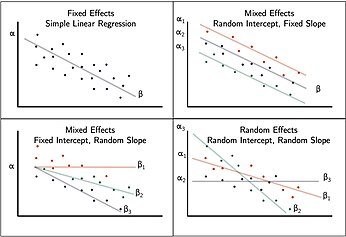
\includegraphics{fig/mixedeffects.jpeg}

\textbf{Reading}

\begin{itemize}
\tightlist
\item
  Galecki \& Burzykowski (2013). Linear Mixed Effects Models using R.
\item
  Fox J (2008). Applied Regression Analysis and Generalized Linear
  Models 2nd ed.
\item
  Wood, S. \emph{Generalized Additive Models}. Ch 2.
\item
  \url{https://m-clark.github.io/mixed-models-with-R/random_intercepts.html}
\item
  \url{https://cran.r-project.org/web/packages/lme4/vignettes/lmer.pdf}
\end{itemize}

\hypertarget{overview}{%
\subsection*{\texorpdfstring{\textbf{Overview}}{Overview}}\label{overview}}
\addcontentsline{toc}{subsection}{\textbf{Overview}}

In this module, you'll learn how to model data with hierarchical or
correlated structures using \textbf{linear mixed models (LMMs).} These
models extend standard regression to handle repeated measures or nested
data structures, commonly found in longitudinal and multilevel public
health data.

\textbf{After completing this module, you will be able to:}

\begin{itemize}
\item
  Identify when LMMs are appropriate
\item
  Distinguish between fixed and random effects
\item
  Fit and interpret random intercept and random slope models in R
\item
  Understand concepts like shrinkage, intraclass correlation, and BLUPs
\item
  Hierarchical formulation of random effects models
\end{itemize}

\hypertarget{motivation-and-examples-1}{%
\subsection*{Motivation and Examples}\label{motivation-and-examples-1}}
\addcontentsline{toc}{subsection}{Motivation and Examples}

\begin{tcolorbox}[enhanced jigsaw, breakable, colbacktitle=quarto-callout-important-color!10!white, left=2mm, colframe=quarto-callout-important-color-frame, opacityback=0, coltitle=black, colback=white, rightrule=.15mm, title=\textcolor{quarto-callout-important-color}{\faExclamation}\hspace{0.5em}{Motivation:}, titlerule=0mm, opacitybacktitle=0.6, leftrule=.75mm, toprule=.15mm, arc=.35mm, bottomtitle=1mm, toptitle=1mm, bottomrule=.15mm]

Correlated data structures arise when multiple observations are taken
from the same unit or group: Examples include:

\begin{itemize}
\tightlist
\item
  \textbf{Longitudinal data:} Repeated measures data on each subject

  \begin{itemize}
  \tightlist
  \item
    \(y_{it}\) denotes the measure at time \(t\) for unit \(i\).
  \end{itemize}
\item
  \textbf{Clustered or multilevel data:} Observations within nested
  group structures.

  \begin{itemize}
  \tightlist
  \item
    A collection of units from a population of similar units, e.g.,
    \(y_{ij}\) denotes measure from person \(i\) in demographic group
    \(j\).
  \end{itemize}
\end{itemize}

Ignoring this structure can lead to biased estimates and invalid
inference.

\end{tcolorbox}

\textbf{Motivating Example: The TLC Study:}

The Treatment of Lead-Exposed Children (TLC) was examined using a
placebo-controlled randomized study of succimer (a chelating agent) in
children with blood lead levels of 20-44 micrograms/dL. These data
consist of four repeated measurements of blood lead levels obtained at
baseline (or week 0) , week 1, week 4, and week 6 on 100 children who
were randomly assigned to chelation treament with succimer or placebo.

\begin{longtable}[]{@{}ll@{}}
\toprule\noalign{}
Variable & Description \\
\midrule\noalign{}
\endhead
\bottomrule\noalign{}
\endlastfoot
\texttt{id} & child identifier \\
\texttt{treatment} & succimer or placebo \\
\texttt{week} & measurement week \\
\texttt{lead} & lead level (outcome) \\
\end{longtable}

\begin{Shaded}
\begin{Highlighting}[]
\NormalTok{tlcdata }\OtherTok{\textless{}{-}} \FunctionTok{readRDS}\NormalTok{(}\StringTok{"data/tlc.RDS"}\NormalTok{)}
\FunctionTok{head}\NormalTok{(tlcdata)}
\end{Highlighting}
\end{Shaded}

\begin{verbatim}
    id treatment week lead
1    1   placebo    0 30.8
101  1   placebo    1 26.9
201  1   placebo    4 25.8
301  1   placebo    6 23.8
2    2  succimer    0 26.5
102  2  succimer    1 14.8
\end{verbatim}


\includegraphics{Module_1A_LMM_files/figure-pdf/unnamed-chunk-4-1.pdf}

\hypertarget{why-not-ols-the-wrong-approach}{%
\subsection*{\texorpdfstring{Why Not OLS? \ul{\textbf{The wrong
approach}}}{Why Not OLS? The wrong approach}}\label{why-not-ols-the-wrong-approach}}
\addcontentsline{toc}{subsection}{Why Not OLS? \ul{\textbf{The wrong
approach}}}

If we ignore clustering and fit the standard linear regression (OLS): \[
\begin{align*}
y_{ij}& = \beta_0 + \beta_1 x_{ij} + \epsilon_{ij}\\
\epsilon_{ij} & \overset{iid}{\sim} N(0, \sigma^2)
\end{align*}
\] we assume that all observations are independent.

But repeated measurements from the same child are \textbf{not}
independent.

\begin{Shaded}
\begin{Highlighting}[]
\NormalTok{fit.lm }\OtherTok{=} \FunctionTok{lm}\NormalTok{(lead }\SpecialCharTok{\textasciitilde{}}\NormalTok{ week, }\AttributeTok{data =}\NormalTok{ tlcdata)}
\FunctionTok{summary}\NormalTok{(fit.lm)}
\end{Highlighting}
\end{Shaded}

\begin{verbatim}

Call:
lm(formula = lead ~ week, data = tlcdata)

Residuals:
    Min      1Q  Median      3Q     Max 
-19.775  -3.749   0.328   4.454  43.330 

Coefficients:
            Estimate Std. Error t value Pr(>|t|)    
(Intercept)  22.9760     0.6079  37.793   <2e-16 ***
week         -0.4010     0.1670  -2.401   0.0168 *  
---
Signif. codes:  0 '***' 0.001 '**' 0.01 '*' 0.05 '.' 0.1 ' ' 1

Residual standard error: 7.966 on 398 degrees of freedom
Multiple R-squared:  0.01428,   Adjusted R-squared:  0.0118 
F-statistic: 5.765 on 1 and 398 DF,  p-value: 0.01681
\end{verbatim}

\textbf{What assumptions of OLS are we violating?}

\begin{itemize}
\item
  \(\hat{\beta}_1\) is an unbiased and consistent estimator of
  \(\beta_1\).
\item
  Errors are not independent which leads to incorrect standard error
  estimates.
\item
  \(\sigma^2\) conflates within and between child variability.
\item
  Limitations: You cannot forecast individual trajectories.
\end{itemize}

\hypertarget{the-better-approach-introducing-linear-mixed-models}{%
\section*{\texorpdfstring{\ul{The Better Approach: Introducing Linear
Mixed
Models}}{The Better Approach: Introducing Linear Mixed Models}}\label{the-better-approach-introducing-linear-mixed-models}}
\addcontentsline{toc}{section}{\ul{The Better Approach: Introducing
Linear Mixed Models}}

\markright{\ul{The Better Approach: Introducing Linear Mixed Models}}

LMMs are extensions of regression in which intercepts and/or slopes are
allowed to vary across individual units. They were developed to deal
with correlated and/or nested data.

Taking our motivating example, we can assign a separate intercept for
each child:

\[
\begin{align*}
y_{ij} &= \beta_{0i} + \beta_1 x_{ij} + \epsilon_{ij}, \\
\epsilon_{ij} & \overset{iid}{\sim} N(0, \sigma^2)
\end{align*}
\]

\textbf{Interpretation:}

\begin{itemize}
\tightlist
\item
  \(\beta_{0i}\) is the \textcolor{red}{child-specific} weight at zero
  and \(\beta_1\) is the constant slope.
\item
  \(\sigma^2\) captures \textcolor{red}{within} child variability.
\item
  The mix of random and fixed effects = mixed modeling.
\end{itemize}

\begin{longtable}[]{@{}
  >{\raggedright\arraybackslash}p{(\columnwidth - 4\tabcolsep) * \real{0.3333}}
  >{\raggedright\arraybackslash}p{(\columnwidth - 4\tabcolsep) * \real{0.3333}}
  >{\raggedright\arraybackslash}p{(\columnwidth - 4\tabcolsep) * \real{0.3333}}@{}}
\toprule\noalign{}
\begin{minipage}[b]{\linewidth}\raggedright
\textbf{Effect Type}
\end{minipage} & \begin{minipage}[b]{\linewidth}\raggedright
\textbf{Definition}
\end{minipage} & \begin{minipage}[b]{\linewidth}\raggedright
\textbf{Example}
\end{minipage} \\
\midrule\noalign{}
\endhead
\bottomrule\noalign{}
\endlastfoot
Fixed & Population-average effects & Effect of week on lead \\
Random & Child-specific deviation & Child-specific intercept
\(\beta_{0i}\) \\
Random & Child-week deviation & Child-week error \(\epsilon_{ij}\) \\
\end{longtable}

A limitation to this approach is we are estimating a lot of parameters:
Subject specific coefficients don't leverage population information and
have less precision because of smaller sample sizes.

In addition, we cannot forecast the outcome of a \textcolor{red}{new}
child.

\hypertarget{random-intercept-model}{%
\subsection*{Random Intercept Model}\label{random-intercept-model}}
\addcontentsline{toc}{subsection}{Random Intercept Model}

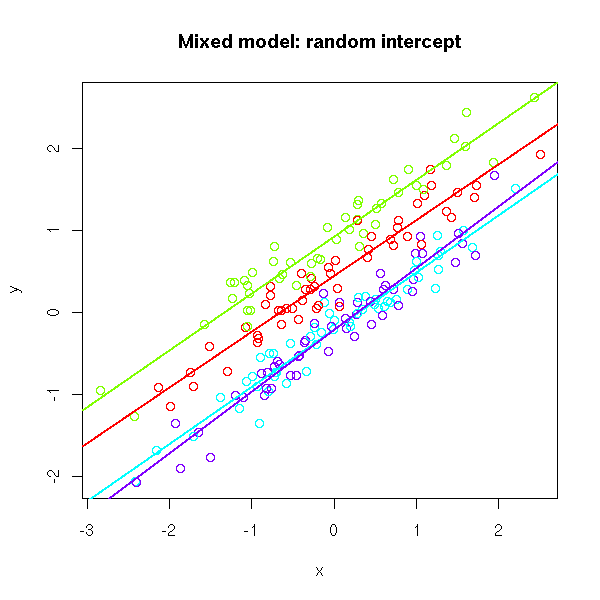
\includegraphics[width=6.25in,height=\textheight]{fig/randomint.png}

Consider the random intercept model with a vector of predictors
\(x_{ij}\):

\[
\begin{align*}
y_{ij} &=\mu + \theta_i + x_{ij}^T \beta + \epsilon_{ij}\\
\epsilon_{ij} & \overset{iid}{\sim} N(0, \sigma^2)\\
\theta_i & \overset{iid}{\sim} N(0, \tau^2) \\
\theta_i& \perp \epsilon_{ij}
\end{align*}
\]

\begin{itemize}
\item
  \(\mu\) = overall intercept (population mean when \(x_{ij}=0\)).
\item
  \(\theta_i\) = child specific difference from \(\mu\).
\item
  \(\beta_{0i} = \mu + \theta_i\) participant specific intercept or
  child specific average.
\item
  \(\beta\) = coefficient that does not vary across participants.
\item
  \(\tau^2\) = between group variability.
\item
  \(\sigma^2\) = residual variance or within group variability
  ``measurement error''.
\end{itemize}

\textbf{Model Assumptions:}

\begin{itemize}
\item
  We assume the random intercept and random errors are independent
  \(\theta_i \perp \epsilon_{ij}\) for all \(i\) and \(j\).
\item
  We assume the random intercepts are normally distributed
  \(\theta_i \sim N(0, \tau^2)\).
\end{itemize}

\hypertarget{properties-of-the-random-intercept-model}{%
\subsection*{Properties of the Random Intercept
Model}\label{properties-of-the-random-intercept-model}}
\addcontentsline{toc}{subsection}{Properties of the Random Intercept
Model}

\emph{Use the expandable panels below to explore key statistical
properties and their derivations.}

\begin{tcolorbox}[enhanced jigsaw, rightrule=.15mm, breakable, left=2mm, colframe=quarto-callout-tip-color-frame, opacityback=0, leftrule=.75mm, toprule=.15mm, colback=white, arc=.35mm, bottomrule=.15mm]

\textbf{What is the overall (average) trend?}\vspace{2mm}

The population-level mean is computed by taking expectations over both
random effects:

\[
\mathbb{E}[y_{ij}] = \mathbb{E}_{\theta_i, \epsilon_{ij}}[(\mu + \theta_i) + \beta x_{ij} + \epsilon_{ij}] = \mu + \beta x_{ij}
\]

\textbf{Interpretation}: This is the average regression line across all
individuals. The random intercept \(\theta_i\) averages to 0.

\end{tcolorbox}

\begin{tcolorbox}[enhanced jigsaw, rightrule=.15mm, breakable, left=2mm, colframe=quarto-callout-tip-color-frame, opacityback=0, leftrule=.75mm, toprule=.15mm, colback=white, arc=.35mm, bottomrule=.15mm]

\textbf{What is the total variability around the overall
trend?}\vspace{2mm}

Using the law of total variance:

\[
\begin{align*}
\text{Var}(y_{ij}) & = \text{Var}(\mu + \theta_i + \beta x_{ij} + \epsilon_{ij})\\
&  = \text{Var}(\theta_i) + \text{Var}(\epsilon_{ij}) \\
& = \tau^2 + \sigma^2
\end{align*}
\]

\textbf{Interpretation}: Total variability includes both between-subject
variance (\(\tau^2\)) and within-subject variance (\(\sigma^2\)).

\end{tcolorbox}

\begin{tcolorbox}[enhanced jigsaw, rightrule=.15mm, breakable, left=2mm, colframe=quarto-callout-tip-color-frame, opacityback=0, leftrule=.75mm, toprule=.15mm, colback=white, arc=.35mm, bottomrule=.15mm]

\textbf{What is the conditional (group-specific) trend?}\vspace{2mm}

Conditioning on \(\theta_i\):

\[ 
\mathbb{E}[y_{ij} \mid \theta_i] = (\mu + \theta_i) +  x_{ij}^T \beta
\]

\textbf{Interpretation}: Each subject gets their own intercept offset
(\(\theta_i\)), producing a personalized regression line.

\end{tcolorbox}

\begin{tcolorbox}[enhanced jigsaw, rightrule=.15mm, breakable, left=2mm, colframe=quarto-callout-tip-color-frame, opacityback=0, leftrule=.75mm, toprule=.15mm, colback=white, arc=.35mm, bottomrule=.15mm]

\textbf{What is the conditional (within-group) residual
variance?}\vspace{2mm}

Conditional on \(\theta_i\), the only random component is
\(\epsilon_{ij}\):

\[
\text{Var}(y_{ij} \mid \theta_i) = \text{Var}(\epsilon_{ij}) = \sigma^2 
\]

\textbf{Interpretation}: Within each group (or individual), the variance
reflects only the measurement error or residual noise.

\end{tcolorbox}

\hypertarget{fitting-a-mixed-effects-model-with-a-random-intercept-in-r}{%
\subsection*{Fitting a mixed effects model with a random intercept in
R:}\label{fitting-a-mixed-effects-model-with-a-random-intercept-in-r}}
\addcontentsline{toc}{subsection}{Fitting a mixed effects model with a
random intercept in R:}

\begin{Shaded}
\begin{Highlighting}[]
\FunctionTok{library}\NormalTok{(lmerTest)}
\NormalTok{fit.randomeffects }\OtherTok{=} \FunctionTok{lmer}\NormalTok{(lead }\SpecialCharTok{\textasciitilde{}}\NormalTok{ week }\SpecialCharTok{+}\NormalTok{ (}\DecValTok{1}\SpecialCharTok{|}\NormalTok{id), }\AttributeTok{data =}\NormalTok{ tlcdata)}
\FunctionTok{summary}\NormalTok{(fit.randomeffects)}
\end{Highlighting}
\end{Shaded}

\begin{verbatim}
Linear mixed model fit by REML. t-tests use Satterthwaite's method [
lmerModLmerTest]
Formula: lead ~ week + (1 | id)
   Data: tlcdata

REML criterion at convergence: 2695.1

Scaled residuals: 
    Min      1Q  Median      3Q     Max 
-2.6337 -0.3461  0.0601  0.4131  6.1167 

Random effects:
 Groups   Name        Variance Std.Dev.
 id       (Intercept) 29.63    5.444   
 Residual             33.98    5.829   
Number of obs: 400, groups:  id, 100

Fixed effects:
            Estimate Std. Error       df t value Pr(>|t|)    
(Intercept)  22.9760     0.7030 161.6442  32.683  < 2e-16 ***
week         -0.4010     0.1222 299.0000  -3.281  0.00116 ** 
---
Signif. codes:  0 '***' 0.001 '**' 0.01 '*' 0.05 '.' 0.1 ' ' 1

Correlation of Fixed Effects:
     (Intr)
week -0.478
\end{verbatim}

\textbf{Model Interpretation:} The fixed effect captures the global or
average change in lead level for every one unit change in time, i.e.,
from week 1 to week 2, \(\hat{\beta}_1 = -0.410\), meaning that there is
an average 0.4 decrease in lead for every unit increase in week which
was found to be statistically significant \(p<0.01\).

Now the intercept 22.97 corresponds to the \ul{population-average lead
at week 0}.

The SE of the slope \(se(\hat{\beta_1}) = 0.122\) capturing uncertainty
associated with the estimate.

The random effect of child \(\beta_{0i}\) allows for child-specific
random intercepts, where the variance of the intercepts is 29.63.

\hypertarget{covariance-structure-and-matrix-form}{%
\subsection*{Covariance Structure and Matrix
Form}\label{covariance-structure-and-matrix-form}}
\addcontentsline{toc}{subsection}{Covariance Structure and Matrix Form}

A random intercept model is also known as a \textcolor{red}{two-level}
variance component model:

\begin{itemize}
\item
  \(\theta_i\) is a \textbf{random intercept} shared by all observations
  in group \(i\) and has a ``intercept-specific'' error \(\tau^2\).
\item
  \(\epsilon_{ij}\) is the \textbf{individual-level residual error}.
\end{itemize}

\begin{center}\rule{0.5\linewidth}{0.5pt}\end{center}

\hypertarget{derivation-textcovy_ij-y_ik-for-j-ne-k}{%
\subsubsection*{\texorpdfstring{Derivation:
\(\text{Cov}(y_{ij}, y_{ik})\) for
\(j \ne k\)}{Derivation: \textbackslash text\{Cov\}(y\_\{ij\}, y\_\{ik\}) for j \textbackslash ne k}}\label{derivation-textcovy_ij-y_ik-for-j-ne-k}}
\addcontentsline{toc}{subsubsection}{Derivation:
\(\text{Cov}(y_{ij}, y_{ik})\) for \(j \ne k\)}

We now derive the \textbf{covariance} between two observations from the
same person \(i\). Let's expand both observations:

\[
\begin{aligned}
y_{ij} &= \mu + \theta_i + \beta x_{ij} + \epsilon_{ij} \\
y_{ik} &= \mu + \theta_i + \beta x_{ik} + \epsilon_{ik}
\end{aligned}
\]

Then,

\[
\text{Cov}(y_{ij}, y_{ik}) = \text{Cov}(\theta_i + \epsilon_{ij},\ \theta_i + \epsilon_{ik})
\]

Using bilinearity of covariance:

\[
= \text{Cov}(\theta_i, \theta_i) + \text{Cov}(\theta_i, \epsilon_{ik}) + \text{Cov}(\epsilon_{ij}, \theta_i) + \text{Cov}(\epsilon_{ij}, \epsilon_{ik})
\]

Now plug in the assumptions:

\begin{itemize}
\tightlist
\item
  \(\text{Var}(\theta_i) = \tau^2\)
\item
  \(\text{Cov}(\theta_i, \epsilon_{ij}) = 0\)
\item
  \(\text{Cov}(\epsilon_{ij}, \epsilon_{ik}) = 0\) for \(j \ne k\)
\end{itemize}

So:

\[
 \text{Cov}(y_{ij}, y_{ik}) = \tau^2\quad  ✅ 
\] Observations from the same group/cluster share the same random
intercept \(\theta_i\), which introduces positive correlation.

\begin{center}\rule{0.5\linewidth}{0.5pt}\end{center}

\hypertarget{derivation-textvary_ij}{%
\subsubsection*{\texorpdfstring{Derivation:
\(\text{Var}(y_{ij})\)}{Derivation: \textbackslash text\{Var\}(y\_\{ij\})}}\label{derivation-textvary_ij}}
\addcontentsline{toc}{subsubsection}{Derivation: \(\text{Var}(y_{ij})\)}

Let's derive the total (marginal) variability of an individual
observation \(y_{ij}\) around the population mean, after averaging over
the distribution of subjects. By the law of total variance:

Total variance = between-group variance + within-group variance. \[
\text{Var}(y_{ij}) = \text{Var}(\theta_i + \epsilon_{ij}) = \tau^2 + \sigma^2\quad ✅ 
\]
------------------------------------------------------------------------

\hypertarget{derivation-textcovy_ij-y_kj}{%
\subsubsection*{\texorpdfstring{Derivation:
\(\text{Cov}(y_{ij}, y_{kj})\)}{Derivation: \textbackslash text\{Cov\}(y\_\{ij\}, y\_\{kj\})}}\label{derivation-textcovy_ij-y_kj}}
\addcontentsline{toc}{subsubsection}{Derivation:
\(\text{Cov}(y_{ij}, y_{kj})\)}

The covariance between two different subjects is assumed to be zero: \[
\text{Cov}(y_{ij}, y_{kj}) = Cov(\theta_i + \epsilon_{ij}, \theta_k + \epsilon_{kj}) = 0 \quad ✅ 
\]

\begin{center}\rule{0.5\linewidth}{0.5pt}\end{center}

\hypertarget{covariance-matrix}{%
\subsubsection*{Covariance Matrix}\label{covariance-matrix}}
\addcontentsline{toc}{subsubsection}{Covariance Matrix}

Suppose we observe two individuals, each measured at three time points:

\begin{itemize}
\tightlist
\item
  Subject 1: \(y_{11}, y_{12}, y_{13}\)
\item
  Subject 2: \(y_{21}, y_{22}, y_{23}\)
\end{itemize}

The \textbf{marginal covariance matrix} \(\text{Cov}(\mathbf{y})\) for
the stacked vector:

\[
\mathbf{y} = 
\begin{bmatrix}
y_{11} \\
y_{12} \\
y_{13} \\
y_{21} \\
y_{22} \\
y_{23}
\end{bmatrix}
\]

is:

\[
\text{Cov}(\mathbf{y}) =
\begin{bmatrix}
\tau^2 + \sigma^2 & \tau^2 & \tau^2 & 0 & 0 & 0 \\
\tau^2 & \tau^2 + \sigma^2 & \tau^2 & 0 & 0 & 0 \\
\tau^2 & \tau^2 & \tau^2 + \sigma^2 & 0 & 0 & 0 \\
0 & 0 & 0 & \tau^2 + \sigma^2 & \tau^2 & \tau^2 \\
0 & 0 & 0 & \tau^2 & \tau^2 + \sigma^2 & \tau^2 \\
0 & 0 & 0 & \tau^2 & \tau^2 & \tau^2 + \sigma^2 \\
\end{bmatrix}
\]

\begin{itemize}
\tightlist
\item
  Within a subject, all pairs of outcomes have covariance \(\tau^2\).
\item
  Between subjects, outcomes are independent (covariance = 0).
\item
  Diagonal entries reflect total variance: \(\tau^2 + \sigma^2\).
\end{itemize}

This structure is known as \textbf{compound symmetry} within each
subject (constant pairwise correlation), and \textbf{block-diagonal}
across subjects.

\begin{center}\rule{0.5\linewidth}{0.5pt}\end{center}

\hypertarget{random-intercept-model-in-matrix-form}{%
\subsection*{Random Intercept Model in Matrix
Form}\label{random-intercept-model-in-matrix-form}}
\addcontentsline{toc}{subsection}{Random Intercept Model in Matrix Form}

Consider the mixed model with random intercepts for \(n\) groups and
define \(N = \sum_{i=1}^n r_i\).

\[
\mathbf{y} = \mathbf{Z} \mathbf{\theta} + \mathbf{X}\mathbf{\beta} + \mathbf{\epsilon}
\]

where

\begin{itemize}
\item
  \(\mathbf{y} = N \times 1\) vector of response
\item
  \(\mathbf{Z} = N \times n\) design matrix of indicator variables for
  each group.
\item
  \(\mathbf{\theta} = n \times 1\) vector of random intercepts.
\item
  \(\mathbf{X} = N\times p\) design matrix of fixed effects (including
  overall intercept).
\item
  \(\mathbf{\beta} = p\times 1\) vector of fixed effects.
\item
  \(\mathbf{\epsilon} = N \times 1\) vector of residual error.
\end{itemize}

\begin{tcolorbox}[enhanced jigsaw, rightrule=.15mm, breakable, left=2mm, colframe=quarto-callout-note-color-frame, opacityback=0, leftrule=.75mm, toprule=.15mm, colback=white, arc=.35mm, bottomrule=.15mm]

\textbf{Intraclass Correlation}\vspace{2mm}

Note that the within-group covariance is
\(Cov(y_{ij}, y_{ij'}) = \tau^2\). So the correlation between
observations within the same group is:

\[
\rho = Corr(y_{ij}, y_{ij'}) = \frac{\tau^2}{\tau^2 + \sigma^2} \text{ for all }j \neq j'. 
\]

\begin{itemize}
\tightlist
\item
  The value \(\rho\) is often called the
  \textcolor{red}{intraclass correlation}. It measures the degree of
  similarity among same-group observations
  \textcolor{blue}{compared to the residual error} \(\sigma^2\).
\item
  Describes how strongly units in the same group resemble eachother.
\item
  \(\rho \rightarrow 0\) when \(\tau^2 \rightarrow 0\) (i.e.~same
  intercept)
\item
  \(\rho \rightarrow 0\) when \(\sigma^2 \rightarrow \infty\) (i.e.,
  growing measurement error).
\item
  \(\rho \rightarrow 1\) when \(\tau^2 \rightarrow \infty\) (i.e., large
  separation in intercepts).
\item
  \(\rho \rightarrow 1\) when \(\sigma^2 \rightarrow 0\) (i.e., zero
  measurement error).
\item
  The above ICC has an exchangeable structure because the correlation is
  constant between \emph{any pair} of within-group observations.
\end{itemize}

\end{tcolorbox}

\hypertarget{simulation-varying-between-subject-variability}{%
\subsection*{Simulation Varying Between Subject
Variability}\label{simulation-varying-between-subject-variability}}
\addcontentsline{toc}{subsection}{Simulation Varying Between Subject
Variability}

We simulate data for child \(i\) in week \(j\) using the formula below.
We denote simulated quantities using \(\tilde{.}\). Note below we vary
the degree of between subject variance (heterogeneity) \(\tau^2\).

\[
\begin{align*}
\tilde{y}_{ij} & = 22.976 - 0.4 \times \text{week}_{ij} + \tilde{\theta}_i + \tilde{\epsilon}_{ij}\\
\tilde{\theta}_i & \sim N(0, \tau^2), \quad \tau = (0.5, 16, 100)\\
\tilde{\epsilon}_{ij} & \sim N(0, \sigma^2), \quad \sigma^2 = 4
\end{align*}
\]


\includegraphics{Module_1A_LMM_files/figure-pdf/unnamed-chunk-7-1.pdf}

\hypertarget{simulation-varying-sources-of-error}{%
\subsection*{Simulation Varying Sources of
Error}\label{simulation-varying-sources-of-error}}
\addcontentsline{toc}{subsection}{Simulation Varying Sources of Error}

We simulate repeated outcomes for child \(i\) at week \(j\) again under
a random--intercept model with a fixed trend over time and three
different levels of \textbf{within-child} noise \(\sigma^2\):

\[
\begin{align*}
\tilde{y}_{ij} & = 22.976 - 0.4 \times \text{week}_{ij} + \tilde{\theta}_i + \tilde{\epsilon}_{ij}\\
\tilde{\theta}_i & \sim N(0, \tau^2), \quad \tau^2 = 16\\
\tilde{\epsilon}_{ij} & \sim N(0, \sigma^2), \quad \sigma^2 = (0.5, 16, 100)
\end{align*}
\]


\includegraphics{Module_1A_LMM_files/figure-pdf/unnamed-chunk-8-1.pdf}

\hypertarget{section}{%
\section*{\texorpdfstring{\textcolor{purple}{Summary}}{}}\label{section}}
\addcontentsline{toc}{section}{\textcolor{purple}{Summary}}

\markright{\textcolor{purple}{Summary}}

\begin{longtable}[]{@{}
  >{\raggedright\arraybackslash}p{(\columnwidth - 2\tabcolsep) * \real{0.5000}}
  >{\raggedright\arraybackslash}p{(\columnwidth - 2\tabcolsep) * \real{0.5000}}@{}}
\toprule\noalign{}
\begin{minipage}[b]{\linewidth}\raggedright
\textbf{Section}
\end{minipage} & \begin{minipage}[b]{\linewidth}\raggedright
\textbf{Description}
\end{minipage} \\
\midrule\noalign{}
\endhead
\bottomrule\noalign{}
\endlastfoot
\textbf{Motivation} & Repeated/clustered data (e.g., TLC: children
measured over weeks) create within-subject correlation that standard OLS
ignores. \\
\textbf{Why not OLS?} & OLS fit
\(y_{ij}=\beta_0+\beta_1 x_{ij}+\epsilon_{ij}\) incorrectly assumes
independence. Slope can be unbiased, but standard errors are wrong;
\(\sigma^2\) mixes within/between variability. \\
\textbf{Model (random intercept)} &
\(y_{ij}=\mu+\theta_i+x_{ij}^{\top}\beta+\epsilon_{ij}\), with
\(\epsilon_{ij}\sim N(0,\sigma^2)\), \(\theta_i\sim N(0,\tau^2)\), and
\(\theta_i\perp \epsilon_{ij}\). \(\mu\) = overall intercept;
\(\theta_i\) = child-specific intercept shift; \(\beta\) = fixed-effect
slopes. \\
\textbf{Mean \& variance} & Population mean:
\(\mathbb{E}[y_{ij}]=\mu+\beta^{\top}x_{ij}\). Conditional mean:
\(\mathbb{E}[y_{ij}\mid \theta_i]=(\mu+\theta_i)+\beta^{\top}x_{ij}\).
Marginal variance: \(\operatorname{Var}(y_{ij})=\tau^2+\sigma^2\).
Conditional variance:
\(\operatorname{Var}(y_{ij}\mid \theta_i)=\sigma^2\). \\
\textbf{Covariances} & Same subject, different times:
\(\operatorname{Cov}(y_{ij},y_{ik})=\tau^2\) for \(j\neq k\). Different
subjects: \(\operatorname{Cov}(y_{ij},y_{kj})=0\) for \(i\neq k\).
Implies compound symmetry within subject and block-diagonal overall
covariance. \\
\textbf{Matrix form} & \(y=Z\theta+X\beta+\epsilon\), where \(Z\) maps
observations to subject intercepts, \(X\) is fixed-effects design. \\
\textbf{Intraclass correlation} &
\(\rho=\dfrac{\tau^2}{\tau^2+\sigma^2}\): proportion of total variance
due to between-subject differences; larger \(\tau^2\) or smaller
\(\sigma^2\) \(\Rightarrow\) larger within-subject correlation. \\
\textbf{Simulation takeaways} & Varying \(\tau^2\) (between-subject
variance) changes separation between subject-specific lines and
increases ICC. Varying \(\sigma^2\) (within-subject noise) widens
scatter around each subject's line and reduces ICC. \\
\textbf{Fitting \& interpretation (R)} &
\texttt{lmer(lead\ \textasciitilde{}\ week\ +\ (1\textbar{}id),\ data\ =\ tlcdata)}
fits the random-intercept model. Fixed effect of \texttt{week} = average
change per week; \(\hat\tau^2\) = between-child variance;
\(\hat\sigma^2\) = within-child variance. \\
\end{longtable}

\bookmarksetup{startatroot}

\hypertarget{module-1b-linear-mixed-models}{%
\chapter*{Module 1B Linear Mixed
Models}\label{module-1b-linear-mixed-models}}
\addcontentsline{toc}{chapter}{Module 1B Linear Mixed Models}

\markboth{Module 1B Linear Mixed Models}{Module 1B Linear Mixed Models}

\begin{verbatim}
Warning: package 'dplyr' was built under R version 4.4.3
\end{verbatim}

\hypertarget{partial-pooling-blup-borrowing-strength-across-subjects}{%
\section*{Partial Pooling (BLUP): Borrowing Strength Across
Subjects}\label{partial-pooling-blup-borrowing-strength-across-subjects}}
\addcontentsline{toc}{section}{Partial Pooling (BLUP): Borrowing
Strength Across Subjects}

\markright{Partial Pooling (BLUP): Borrowing Strength Across Subjects}

In random--intercept models, each subject's intercept \(\theta_i\) is
not estimated in isolation. Instead, it is \ul{\textbf{partially
pooled}} toward the overall mean: subjects with few observations (or
noisier measurements) get \textbf{more shrinkage}, while subjects with
lots of precise data get \textbf{less}. The resulting predictor is the
\textbf{Best Linear Unbiased Predictor (BLUP)}---a weighted average of
the subject's sample mean and the population mean, with weights
determined by the \textbf{within-subject variance} \(\sigma^2\), the
\textbf{between-subject variance} \(\tau^2\), and the subject's sample
size \(n_i\). This ``borrowing strength'' across subjects stabilizes
subject-specific estimates and improves out-of-sample prediction.

\hypertarget{the-joint-density}{%
\subsubsection*{The Joint Density}\label{the-joint-density}}
\addcontentsline{toc}{subsubsection}{The Joint Density}

\begin{itemize}
\tightlist
\item
  To simplify the derivation first consider a random effects model
  \emph{without} fixed effects:
\end{itemize}

\[
y_{ij} = \theta_i + \epsilon_{ij}, \quad \theta_i \overset{iid}{\sim} N(0, \tau^2), \quad \epsilon_{ij} \overset{iid}{\sim} N(0, \sigma^2)
\] - To derive the BLUP of \(\theta_i\), we start with the joint density
of the data \emph{and} random effects given by:

\[
f(y_{ij}, \theta_i) = f(y_{ij} \mid \theta_i) \, g(\theta_i),
\]

The conditional density of \(y_{ij}\) given \(\theta_i\) is:

\[
y_{ij} \mid \theta_i \sim N(\theta_i, \sigma^2),
\]

so

\[
f(y_{ij} \mid \theta_i) = \frac{1}{\sqrt{2 \pi \sigma^2}} 
\exp \left( -\frac{(y_{ij} - \theta_i)^2}{2 \sigma^2} \right).
\]

The density of \(\theta_i\) is:

\[
g(\theta_i) = \frac{1}{\sqrt{2 \pi \tau^2}}
\exp \left( - \frac{\theta_i^2}{2 \tau^2} \right).
\]

Putting these together, the joint density of the data and random effects
is given by:

\[
\prod_{ij} f(y_{ij}, \theta_i) = \prod_{i,j} f(y_{ij}|\theta_i) \cdot \prod_i g(\theta_i)
\] Going through the derivation:

\[
f(\{y_{ij}\}, \{\theta_i\}) 
= \prod_{i=1}^m \left[ \left( \prod_{j=1}^{n_i} 
\frac{1}{\sqrt{2 \pi \sigma^2}} 
\exp \left( -\frac{(y_{ij} - \theta_i)^2}{2 \sigma^2} \right) \right) 
\frac{1}{\sqrt{2 \pi \tau^2}} 
\exp \left( - \frac{\theta_i^2}{2 \tau^2} \right) \right].
\]

\hypertarget{best-linear-unbiased-prediction-blup-of-theta_i}{%
\subsection*{\texorpdfstring{Best Linear Unbiased Prediction (BLUP) of
\(\theta_i\)}{Best Linear Unbiased Prediction (BLUP) of \textbackslash theta\_i}}\label{best-linear-unbiased-prediction-blup-of-theta_i}}
\addcontentsline{toc}{subsection}{Best Linear Unbiased Prediction (BLUP)
of \(\theta_i\)}

We aim to find the \textbf{predictor} \(\hat{\theta}_i\) that is linear
in the data, unbiased for \(\theta_i\), and minimizes mean squared error
(the BLUP).

Taking logs (and dropping constants) gives the log-likelihood: \[
\ell(\theta_i) 
= -\frac{1}{2\sigma^2} \sum_{j=1}^{n_i} (y_{ij} - \theta_i)^2 
- \frac{\theta_i^2}{2 \tau^2}.
\]

\textbf{Step 1:} Expand the Quadratic Term Expand the sum of squares: \[
\sum_{j=1}^{n_i} (y_{ij} - \theta_i)^2
= \sum_{j=1}^{n_i} y_{ij}^2 - 2 \theta_i \sum_{j=1}^{n_i} y_{ij} + n_i \theta_i^2.
\]

So:

\[
\ell(\theta_i) 
= -\frac{1}{2\sigma^2} 
\left( \sum_{j=1}^{n_i} y_{ij}^2 - 2 \theta_i \sum_{j=1}^{n_i} y_{ij} + n_i \theta_i^2 \right)
- \frac{\theta_i^2}{2 \tau^2}.
\]

\textbf{Step 2:} Differentiate with Respect to \(\theta_i\) The
derivative is:

\[
\frac{\partial \ell}{\partial \theta_i}
= \frac{\sum_{j=1}^{n_i} y_{ij} - n_i \theta_i}{\sigma^2} - \frac{\theta_i}{\tau^2}.
\]

\textbf{Step 3:} Solve for \(\hat{\theta}_i\) Set the derivative to
zero:

\[
\frac{\sum_{j=1}^{n_i} y_{ij} - n_i \hat{\theta}_i}{\sigma^2} - \frac{\hat{\theta}_i}{\tau^2} = 0.
\]

Multiply by \(\sigma^2\):

\[
\sum_{j=1}^{n_i} y_{ij} - n_i \hat{\theta}_i - \frac{\sigma^2}{\tau^2} \hat{\theta}_i = 0.
\]

Rearrange:

\[
\sum_{j=1}^{n_i} y_{ij} = \hat{\theta}_i \left( n_i + \frac{\sigma^2}{\tau^2} \right).
\]

\begin{tcolorbox}[enhanced jigsaw, rightrule=.15mm, breakable, left=2mm, colframe=quarto-callout-note-color-frame, opacityback=0, leftrule=.75mm, toprule=.15mm, colback=white, arc=.35mm, bottomrule=.15mm]

Thus the \textbf{Best Linear Unbiased Predictor} of \(\theta_i\) is
given by:

\[
\hat{\theta}_i = \frac{\sum_{j=1}^{n_i} y_{ij}}{n_i + \sigma^2 / \tau^2} = \frac{n_i}{n_i + \sigma^2 / \tau^2} \bar{y}_i
\]

where \(\bar{y}_i = \frac{1}{n_i} \sum_{j=1}^{n_i} y_{ij}\).

We can express the BLUP as:

\[
\hat{\theta}_i = B_i \, \bar{y}_i,
\]

where the \textbf{shrinkage factor} is:

\[
B_i = \frac{n_i}{n_i + \sigma^2/\tau^2}.
\]

This shrinkage factor \(B_i\) is the \textbf{precision-weight} placed on
the subject's mean:it forms a \textbf{weighted average} of the subject
mean and the population mean of \(\theta_i\) (which is 0 here),

\[
\hat{\theta}_i = B_i\,\bar{y}_i + (1-B_i)\cdot 0.
\]

\end{tcolorbox}

\textbf{Note that:}

\begin{itemize}
\item
  When \(\tau^2 \to 0\) (no between-group variation),\\
  \(B_i \to 0\) and all random intercepts are shrunk to 0 (the global
  mean).
\item
  When \(\tau^2 \to \infty\) (very large between-group variation),\\
  \(B_i \to 1\) and there is no shrinkage:
  \(\hat{\theta}_i = \bar{y}_i\).
\end{itemize}

\begin{center}\rule{0.5\linewidth}{0.5pt}\end{center}

\hypertarget{hierarchical-formulation}{%
\section*{Hierarchical Formulation}\label{hierarchical-formulation}}
\addcontentsline{toc}{section}{Hierarchical Formulation}

\markright{Hierarchical Formulation}

\textbf{Hierarchical formulation:} A modeling approach where parameters
are allowed to vary by group, but those group parameters are tied
together through a shared distribution, so estimates reflect both the
group's own data and the overall population.

The BLUP shows shrinkage algebraically, but the \textbf{hierarchical
model} explains why it happes: group effects are modeled as draws from a
population, so each estimate combines (1) group data with information
(2) shared across all groups. The amount that each component contributes
depends on both the variance components and the number of observations
within a group.

In a random intercept model, we assume group-specific effects
\(\theta_i\) vary around a common mean \(\mu\):

\[
  y_{ij} = \mu + \theta_i + \epsilon_{ij}, 
  \quad \theta_i \sim N(0, \tau^2), 
  \quad \epsilon_{ij} \sim N(0, \sigma^2),
\]

where:

\begin{itemize}
\tightlist
\item
  \(i = 1, \ldots, m\) indexes groups,
\item
  \(j = 1, \ldots, n_i\) indexes observations within group \(i\),
\item
  \(\tau^2\) is the between-group variance,
\item
  \(\sigma^2\) is the within-group variance.
\end{itemize}

Equivalently, we can reparametrize this as a \textbf{two-level
hierarchical model}:

\begin{itemize}
\tightlist
\item
  \textbf{Level 1 (within-group model):}
  \(y_{ij} \mid \theta_i \sim N( \theta_i, \sigma^2)\).
\item
  \textbf{Level 2 (random effect model):}
  \(\theta_i \sim N(\mu, \tau^2)\).
\end{itemize}

\hypertarget{borrowing-of-information}{%
\subsection*{Borrowing of Information}\label{borrowing-of-information}}
\addcontentsline{toc}{subsection}{Borrowing of Information}

The estimated random intercept \(\hat{\theta}_i\) can be expressed as a
\ul{\textbf{weighted combination}} of the overall mean \(\mu\) and the
group-specific mean \(\bar{y}_i\):

\[
\begin{align*}
\hat{\theta}_i & 
= \frac{(1/\tau^2) \mu + (n_i / \sigma^2) \bar{y}_i}{1/\tau^2 + n_i / \sigma^2},\\
B_i & = \frac{n_i/\sigma^2}{1/\tau^2 + n_i/\sigma^2}\\
\hat{\theta}_i & = (1-B_i) \mu + B_i \bar{y}_i.
\end{align*}
\]

This shows that:

\begin{itemize}
\tightlist
\item
  Groups with \textbf{small} \(n_i\) (few observations) are pulled more
  strongly toward the overall mean \(\mu\),
\item
  Groups with \textbf{large} \(n_i\) rely more on their own mean
  \(\bar{y}_i\).
\item
  When \(n_i\) is small, \(B_i\) is small and there is \textbf{more
  shrinkage}, while large \(n_i\) makes \(B_i\) close to 1 (less
  shrinkage).
\end{itemize}

We can also express \(\hat{\theta}_i\) in terms of the
\textbf{intraclass correlation}: \[
\rho = \frac{\tau^2}{\tau^2 + \sigma^2},
\] leading to:

\[
\hat{\theta}_i 
= \frac{\rho^{-1} \mu + n_i (1-\rho)^{-1} \bar{y}_i}{\rho^{-1} + n_i (1-\rho)^{-1}}.
\]

\textbf{Note that:}

\begin{itemize}
\tightlist
\item
  As \(\tau^2 \to 0\), all \(\hat{\theta}_i \to \mu\) (complete
  shrinkage toward the common mean).
\item
  As \(\tau^2 \to \infty\), \(\hat{\theta}_i \to \bar{y}_i\) (no
  shrinkage, group means are used as-is).
\item
  \ul{The amount of shrinkage depends jointly on \(\tau^2\),
  \(\sigma^2\), and \(n_i\).}
\end{itemize}

\begin{center}\rule{0.5\linewidth}{0.5pt}\end{center}

\hypertarget{parameter-estimation}{%
\section*{Parameter Estimation}\label{parameter-estimation}}
\addcontentsline{toc}{section}{Parameter Estimation}

\markright{Parameter Estimation}

We've specified the random-intercept model, its variance components
\((\tau^2,\sigma^2)\), and seen partial pooling via BLUPs. The next
question is: \textbf{how do we estimate the population-level parameters}
\((\beta, \sigma^2, \tau^2)\) when observations within a group are
correlated**? Because the errors are not i.i.d., ordinary least squares
is no longer efficient (and its standard errors are wrong); we must
account for the covariance of \(\mathbf{y}\).

\begin{tcolorbox}[enhanced jigsaw, rightrule=.15mm, breakable, left=2mm, colframe=quarto-callout-note-color-frame, opacityback=0, leftrule=.75mm, toprule=.15mm, colback=white, arc=.35mm, bottomrule=.15mm]

\textbf{Theorem}: In LMMs, the data are \textbf{correlated}: \[
\text{Cov}(\mathbf{y}) = \mathbf{V} \neq \sigma^2 I.
\]

The optimal estimator becomes the \textbf{generalized least squares
(GLS) estimator}:

\[
\hat{\boldsymbol{\beta}} = (\mathbf{X}^T \mathbf{V}^{-1} \mathbf{X})^{-1} \mathbf{X}^T \mathbf{V}^{-1} \mathbf{y}.
\]

for known \(\mathbf{V}\). This is the \textbf{Best Linear Unbiased
Estimator (BLUE)}.

\end{tcolorbox}

To derive the estimator for \((\hat{\sigma}^2, \hat{\tau}^2)\), we can
use a \textbf{maximum likelihood approach} similar to OLS.

The log-likelihood \(l(\sigma^2, \tau^2)\) is:

\[
l(\sigma^2, \tau^2) = \frac{-N}{2} log(2\pi) - \frac{1}{2} log|\mathbf{V}| - \frac{1}{2} (\mathbf{y} - \mathbf{X}\mathbf{\tilde{\beta}})^T\mathbf{V}^{-1} (\mathbf{y} - \mathbf{X}\mathbf{\tilde{\beta}})
\]

Plugging in \(\tilde{\beta}_{GLS} = (X^T V^{-1} X)^{-1}X^T V^{-1}y\), it
is straightforward to maximize the above function over the 2-D domain of
\(\sigma^2\) and \(\tau^2\) to give their MLEs. This method of
substituting \(\beta\) with their MLE fixed at some other parameters is
known as a \textcolor{red}{profile likelihood approach}.

\begin{center}\rule{0.5\linewidth}{0.5pt}\end{center}

\hypertarget{variance-components-reml}{%
\subsection*{Variance Components: REML}\label{variance-components-reml}}
\addcontentsline{toc}{subsection}{Variance Components: REML}

\textbf{Why MLE can be biased for variances.} In the simple Normal model
with unknown mean,

\[
  y_i \sim N(\mu,\sigma^2),\quad i=1,\dots,n,
\]

the \textbf{MLE} of \(\sigma^2\) given by:

\[
  \hat\sigma^2_{\text{ML}}=\frac{1}{n}\sum_{i=1}^n (y_i-\bar y)^2
\] is biased downward:

\[E[\hat\sigma^2_{\text{ML}}]=\frac{n-1}{n}\sigma^2\neq\sigma^2\].

The bias occurs because the sample mean \(\bar{y}\) is itself estimated
from the data. Since one degree of freedom is ``spent'' estimating
\(\mu\), the spread around \(\bar{y}\) systematically underestimates the
true spread around \(\mu\).

\textbf{Restricted (or Residual) Maximum Likelihood} maximizes a
likelihood based only on \textcolor{red}{error contrast}- linear
combinations of the data that contain no information about \(\beta\). By
working with these contrasts, REML avoids ``using up'' degrees of
freedom on estimating \(\beta\), which removes the downward bias in
variance estimates.

\[
l_R(\sigma^2, \tau^2) = l(\sigma^2, \tau^2) -\frac{1}{2} log|X^T V^{-1}X|  
\]

In the simple case of estimating \(\sigma^2\), we have:

\[
\begin{align*}
\hat{\sigma}^2_{ML}& = \frac{1}{n} \sum_i (y_i - \bar{y})^2\\
\hat{\sigma}^2_{REML}& = \frac{1}{n-1} \sum_i (y_i - \bar{y})^2
\end{align*}
\]

which corrects the ML bias by using \(n-1\) (not \(n\)) in the
denominator. This adjustment removes the degrees of freedom used to
estimate \(\beta\), reducing small-sample bias in variance components.

In mixed models, the REML likelihood effectively uses \(n-p\) residual
degrees of freedom, where \(p\) is the number of fixed-effect
parameters.

\begin{itemize}
\tightlist
\item
  \textbf{Practical notes.}

  \begin{itemize}
  \tightlist
  \item
    REML is preferred for \textbf{estimating variance components} and is
    the \textbf{default} in \texttt{lme4::lmer()}
    (\texttt{REML\ =\ TRUE}).\\
  \item
    (Heads-up) When comparing models with \textbf{different
    fixed-effects structures}, fit with \textbf{ML}
    (\texttt{REML\ =\ FALSE}) so the likelihoods are comparable.
  \end{itemize}
\item
  \textbf{Why variance matters for} \(\beta\) in mixed models.\\
  In OLS,
  \(\hat\beta=(\mathbf{X}^\top\mathbf{X})^{-1}\mathbf{X}^\top\mathbf{y}\)
  does \textbf{not} depend on \(\sigma^2\).\\
  In mixed models, the fixed effects are estimated by \textbf{GLS}, \[
  \hat\beta=\big(\mathbf{X}^\top\mathbf{V}^{-1}\mathbf{X}\big)^{-1}\mathbf{X}^\top\mathbf{V}^{-1}\mathbf{y},
  \] where \(\mathbf{V}\) contains the variance components (e.g.,
  \(\sigma^2,\tau^2\)).\\
  Thus, good variance-component estimates (via REML) improve the
  estimation and inference for \(\beta\).
\end{itemize}

\begin{center}\rule{0.5\linewidth}{0.5pt}\end{center}

\hypertarget{motivating-example-the-tlc-data-contd}{%
\subsection*{Motivating Example: The TLC data
cont'd}\label{motivating-example-the-tlc-data-contd}}
\addcontentsline{toc}{subsection}{Motivating Example: The TLC data
cont'd}

Let's revisit the TLC data example to see how these ideas work in
practice.

\begin{Shaded}
\begin{Highlighting}[]
\FunctionTok{library}\NormalTok{(nlme) }
\FunctionTok{library}\NormalTok{(ggplot2)}
\FunctionTok{library}\NormalTok{(dplyr)}
\FunctionTok{library}\NormalTok{(gridExtra) }
\FunctionTok{library}\NormalTok{(lme4)}
\FunctionTok{library}\NormalTok{(broom.mixed)}
\FunctionTok{library}\NormalTok{(modelsummary)}
\end{Highlighting}
\end{Shaded}

\begin{verbatim}
Warning: package 'modelsummary' was built under R version 4.4.3
\end{verbatim}

\begin{Shaded}
\begin{Highlighting}[]
\NormalTok{tlcdata }\OtherTok{\textless{}{-}} \FunctionTok{readRDS}\NormalTok{(}\StringTok{"data/tlc.RDS"}\NormalTok{)}

\NormalTok{tlc.ml }\OtherTok{\textless{}{-}} \FunctionTok{lmer}\NormalTok{(lead }\SpecialCharTok{\textasciitilde{}}\NormalTok{ week }\SpecialCharTok{+}\NormalTok{ (}\DecValTok{1}\SpecialCharTok{|}\NormalTok{id), }\AttributeTok{data =}\NormalTok{ tlcdata, }\AttributeTok{REML =}\NormalTok{ F) }\CommentTok{\#ML approach for vars}

\NormalTok{tlc.reml }\OtherTok{\textless{}{-}} \FunctionTok{lmer}\NormalTok{(lead }\SpecialCharTok{\textasciitilde{}}\NormalTok{ week }\SpecialCharTok{+}\NormalTok{ (}\DecValTok{1}\SpecialCharTok{|}\NormalTok{id),  }\AttributeTok{data =}\NormalTok{ tlcdata) }\CommentTok{\#REML (Default) approach for vars}


\CommentTok{\# Fixed effects with CIs}
\NormalTok{fixef\_ml   }\OtherTok{\textless{}{-}} \FunctionTok{tidy}\NormalTok{(tlc.ml,   }\AttributeTok{effects =} \StringTok{"fixed"}\NormalTok{, }\AttributeTok{conf.int =} \ConstantTok{TRUE}\NormalTok{)}
\NormalTok{fixef\_reml }\OtherTok{\textless{}{-}} \FunctionTok{tidy}\NormalTok{(tlc.reml, }\AttributeTok{effects =} \StringTok{"fixed"}\NormalTok{, }\AttributeTok{conf.int =} \ConstantTok{TRUE}\NormalTok{)}

\CommentTok{\# Random{-}effect variances (tau\^{}2, sigma\^{}2)}
\NormalTok{ran\_ml   }\OtherTok{\textless{}{-}} \FunctionTok{tidy}\NormalTok{(tlc.ml,   }\AttributeTok{effects =} \StringTok{"ran\_pars"}\NormalTok{, }\AttributeTok{conf.int =} \ConstantTok{TRUE}\NormalTok{)}
\NormalTok{ran\_reml }\OtherTok{\textless{}{-}} \FunctionTok{tidy}\NormalTok{(tlc.reml, }\AttributeTok{effects =} \StringTok{"ran\_pars"}\NormalTok{, }\AttributeTok{conf.int =} \ConstantTok{TRUE}\NormalTok{)}

\CommentTok{\# Compact side{-}by{-}side summary (coef tables + fit stats)}
\FunctionTok{modelsummary}\NormalTok{(}
  \FunctionTok{list}\NormalTok{(}\StringTok{"ML (full LL)"} \OtherTok{=}\NormalTok{ tlc.ml, }\StringTok{"REML (restricted LL)"} \OtherTok{=}\NormalTok{ tlc.reml),}
  \AttributeTok{estimate  =} \StringTok{"\{estimate\}"}\NormalTok{,}
  \AttributeTok{statistic =} \StringTok{"SE = \{std.error\}, t = \{statistic\}"}\NormalTok{,}
  \AttributeTok{gof\_map =} \FunctionTok{c}\NormalTok{(}\StringTok{"AIC"}\NormalTok{,}\StringTok{"BIC"}\NormalTok{,}\StringTok{"logLik"}\NormalTok{,}\StringTok{"REMLcrit"}\NormalTok{,}\StringTok{"ICC"}\NormalTok{),}
  \AttributeTok{stars =} \ConstantTok{FALSE}\NormalTok{, }\AttributeTok{fmt =} \DecValTok{3}
\NormalTok{)}
\end{Highlighting}
\end{Shaded}

\begin{table}
\centering
\begin{tblr}[         %% tabularray outer open
]                     %% tabularray outer close
{                     %% tabularray inner open
colspec={Q[]Q[]Q[]},
hline{2}={1-3}{solid, black, 0.05em},
hline{10}={1-3}{solid, black, 0.05em},
hline{1}={1-3}{solid, black, 0.08em},
hline{14}={1-3}{solid, black, 0.08em},
column{2-3}={}{halign=c},
column{1}={}{halign=l},
}                     %% tabularray inner close
& ML (full LL) & REML (restricted LL) \\
(Intercept) & \num{22.976} & \num{22.976} \\
& SE = \num{0.700}, t = \num{32.822} & SE = \num{0.703}, t = \num{32.683} \\
week & \num{-0.401} & \num{-0.401} \\
& SE = \num{0.122}, t = \num{-3.287} & SE = \num{0.122}, t = \num{-3.281} \\
sd\_\_(Intercept) & \num{5.411} & \num{5.444} \\
& SE = , t = & SE = , t = \\
sd\_\_Observation & \num{5.819} & \num{5.829} \\
& SE = , t = & SE = , t = \\
AIC & \num{2701.6} & \num{2703.1} \\
BIC & \num{2717.5} & \num{2719.0} \\
Log.Lik. & \num{-1346.781} & \num{-1347.531} \\
REMLcrit &  & \num{2695} \\
\end{tblr}
\end{table}

\begin{center}\rule{0.5\linewidth}{0.5pt}\end{center}

\textcolor{purple}{Summary}

\begin{longtable}[]{@{}
  >{\raggedright\arraybackslash}p{(\columnwidth - 2\tabcolsep) * \real{0.4306}}
  >{\raggedright\arraybackslash}p{(\columnwidth - 2\tabcolsep) * \real{0.5694}}@{}}
\toprule\noalign{}
\begin{minipage}[b]{\linewidth}\raggedright
\textbf{Section}
\end{minipage} & \begin{minipage}[b]{\linewidth}\raggedright
\textbf{Description}
\end{minipage} \\
\midrule\noalign{}
\endhead
\bottomrule\noalign{}
\endlastfoot
\textbf{Partial pooling (BLUP)} & Random--intercept models
\textbf{shrink} subject intercepts toward the population mean. More
shrinkage with \textbf{small} \(n_i\), \textbf{large} \(\sigma^2\), or
\textbf{small} \(\tau^2\). \\
\textbf{BLUP of} \(\theta_i\) (no fixed effects) &
\(\hat{\theta}_i=\dfrac{n_i}{n_i+\sigma^2/\tau^2}\,\bar y_i \equiv B_i\bar y_i\).
Notes: \(\tau^2\!\to\!0 \Rightarrow B_i\!\to\!0\) (shrink to 0);
\(\tau^2\!\to\!\infty \Rightarrow B_i\!\to\!1\) (no shrinkage). \\
\textbf{Hierarchical formulation} &
\(y_{ij}=\mu+\theta_i+\epsilon_{ij}\), with \(\theta_i\sim N(0,\tau^2)\)
and \(\epsilon_{ij}\sim N(0,\sigma^2)\). Two levels: (1)
\(y_{ij}\mid\theta_i\sim N(\mu+\theta_i,\sigma^2)\); (2)
\(\theta_i\sim N(0,\tau^2)\). \\
\textbf{Borrowing of information (weights)} &
\(\hat{\theta}_i=\dfrac{(1/\tau^2)\mu+(n_i/\sigma^2)\bar y_i}{1/\tau^2+n_i/\sigma^2}\).
Small \(n_i\) pulls estimates toward \(\mu\); large \(n_i\) relies more
on \(\bar y_i\). With \(\rho=\tfrac{\tau^2}{\tau^2+\sigma^2}\), an
equivalent weighted form is given in the notes. \\
\textbf{Correlated data → GLS for fixed effects} & With
\(\operatorname{Cov}(\mathbf y)=\mathbf V\) (positive definite),
\(\hat\beta_{GLS}=(\mathbf X^\top\mathbf V^{-1}\mathbf X)^{-1}\mathbf X^\top\mathbf V^{-1}\mathbf y.\)
OLS is the special case \(\mathbf V=\sigma^2\mathbf I\). \\
\textbf{Variance components: ML vs REML} & \textbf{ML} variance
estimates are biased downward (like dividing by \(n\)). \textbf{REML}
maximizes a likelihood of error contrasts that remove fixed-effect
information, reducing small-sample bias (analogue: divide by \(n-p\)).
\textbf{Practice:} use REML for variance components (default in
\texttt{lme4::lmer()}); use ML when comparing models with different
fixed effects. \\
\end{longtable}

\bookmarksetup{startatroot}

\hypertarget{module-1c-random-intercepts-and-slopes}{%
\chapter*{Module 1C Random Intercepts and
Slopes}\label{module-1c-random-intercepts-and-slopes}}
\addcontentsline{toc}{chapter}{Module 1C Random Intercepts and Slopes}

\markboth{Module 1C Random Intercepts and Slopes}{Module 1C Random
Intercepts and Slopes}

\begin{verbatim}
Warning: package 'dplyr' was built under R version 4.4.3
\end{verbatim}

From Random Intercepts to Random Slopes:
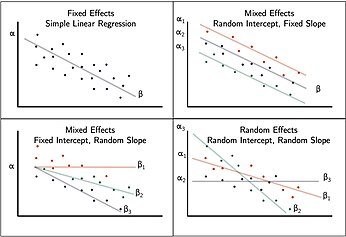
\includegraphics[width=5.3125in,height=\textheight]{fig/mixedeffects.jpeg}

\begin{itemize}
\tightlist
\item
  Consider the mixed effects model with a vector of predictors
  \(x_{ij}\):
\end{itemize}

\[
y_{ij} = (\beta_0 + \theta_{0i}) + (\beta_1 + \theta_{1i}) x_{ij} + \epsilon_{ij}, \quad \epsilon_{ij} \overset{iid}{\sim} N(0, \sigma^2)
\]

\begin{itemize}
\item
  \(\beta_{0i} = \beta_0 + \theta_{0i}\) child specific intercept or
  child specific average.
\item
  \(\beta_{1i} = \beta_1 + \theta_{1i}\) child specific rate of change
  or slope.
\item
  \(\beta_0, \beta_1\) the intercept and slope that does not vary across
  subjects.
\item
  \(\sigma^2\) within subject variability ie measurement error.
\end{itemize}

\hypertarget{random-effects-covariance-structure}{%
\subsection*{Random Effects Covariance
Structure}\label{random-effects-covariance-structure}}
\addcontentsline{toc}{subsection}{Random Effects Covariance Structure}

The random effects are modeled jointly as:

\[
\begin{pmatrix}\theta_{0i} \\ \theta_{1i} \end{pmatrix} \sim N \left( \begin{pmatrix} 0 \\ 0 \end{pmatrix}, \begin{pmatrix} \tau^2_0 & \rho \tau_0 \tau_1 \\ 
\rho \tau_0 \tau_1 & \tau_1^2 \end{pmatrix} \right)
\] where:

\begin{itemize}
\tightlist
\item
  \(\tau_0^2\) is the variance of random intercepts,
\item
  \(\tau_1^2\) is the variance of random slopes,
\item
  \(\rho\) is the correlation between intercepts and slopes.
\end{itemize}

This structure allows us to model not just variation in starting points
(intercepts) and rates of change (slopes), but also how they are related
(e.g., do groups with higher baselines tend to change faster?).

\hypertarget{fitting-the-random-intercept-and-slope-model-in-r}{%
\subsubsection*{Fitting the Random Intercept and Slope model in
R}\label{fitting-the-random-intercept-and-slope-model-in-r}}
\addcontentsline{toc}{subsubsection}{Fitting the Random Intercept and
Slope model in R}

Lets fit the model using the tlc data:

\begin{Shaded}
\begin{Highlighting}[]
\FunctionTok{library}\NormalTok{(ggplot2)}
\FunctionTok{library}\NormalTok{(dplyr)}
\FunctionTok{library}\NormalTok{(gridExtra) }
\FunctionTok{library}\NormalTok{(lme4)}
\NormalTok{tlcdata }\OtherTok{\textless{}{-}} \FunctionTok{readRDS}\NormalTok{(}\StringTok{"data/tlc.RDS"}\NormalTok{)}

\NormalTok{placebo\_data }\OtherTok{=}\NormalTok{ tlcdata }\SpecialCharTok{\%\textgreater{}\%} \FunctionTok{filter}\NormalTok{(treatment }\SpecialCharTok{==} \StringTok{"placebo"}\NormalTok{)}
\NormalTok{fit\_random }\OtherTok{\textless{}{-}} \FunctionTok{lmer}\NormalTok{(lead }\SpecialCharTok{\textasciitilde{}}\NormalTok{ week }\SpecialCharTok{+}\NormalTok{ (week}\SpecialCharTok{|}\NormalTok{id), }\AttributeTok{data =}\NormalTok{ placebo\_data)}
\FunctionTok{summary}\NormalTok{(fit\_random)}
\end{Highlighting}
\end{Shaded}

\begin{verbatim}
Linear mixed model fit by REML ['lmerMod']
Formula: lead ~ week + (week | id)
   Data: placebo_data

REML criterion at convergence: 1053.3

Scaled residuals: 
     Min       1Q   Median       3Q      Max 
-2.20808 -0.49837 -0.02268  0.47100  2.30541 

Random effects:
 Groups   Name        Variance Std.Dev. Corr
 id       (Intercept) 23.3113  4.8282       
          week         0.1581  0.3976   0.02
 Residual              4.5016  2.1217       
Number of obs: 200, groups:  id, 50

Fixed effects:
            Estimate Std. Error t value
(Intercept) 25.68536    0.72018  35.665
week        -0.37213    0.08437  -4.411

Correlation of Fixed Effects:
     (Intr)
week -0.164
\end{verbatim}

\textbf{Interpretation:}

\begin{itemize}
\tightlist
\item
  Child-specific intercept:
  \((\beta_0 + \theta_{0i}) \sim N(25.68, 23.31)\).
\item
  Child-specific slope:
  \((\beta_1 + \theta_{1i}) \sim N(-0.372, 0.158)\).
\item
  The correlation \(\rho\) between \((\beta_{0i}, \beta_{1i}) = 0.02\).
\item
  The fixed effect of week \(\hat{\beta}_1 = -0.372\) is the
  population-average slope. To test whether lead levels change
  significantly over time, use the fixed effect t-test for \(\beta_1\),
  not the spread of the random effects distribution.
\end{itemize}

Below we visualize the individual trajectories based on both fixed
effects and random intercepts and slopes.

\begin{Shaded}
\begin{Highlighting}[]
\FunctionTok{library}\NormalTok{(ggplot2)}
\FunctionTok{ggplot}\NormalTok{(placebo\_data, }\FunctionTok{aes}\NormalTok{(}\AttributeTok{x =}\NormalTok{ week, }\AttributeTok{y =}\NormalTok{ lead, }\AttributeTok{group =}\NormalTok{ id)) }\SpecialCharTok{+}
  \FunctionTok{geom\_point}\NormalTok{(}\AttributeTok{alpha =} \FloatTok{0.5}\NormalTok{) }\SpecialCharTok{+}
  \FunctionTok{geom\_line}\NormalTok{(}\FunctionTok{aes}\NormalTok{(}\AttributeTok{y =} \FunctionTok{predict}\NormalTok{(fit\_random)), }\AttributeTok{color =} \StringTok{"blue"}\NormalTok{) }\SpecialCharTok{+}
  \FunctionTok{labs}\NormalTok{(}\AttributeTok{title =} \StringTok{"Random Intercepts and Slopes by Individual"}\NormalTok{,}
       \AttributeTok{x =} \StringTok{"Week"}\NormalTok{, }\AttributeTok{y =} \StringTok{"Lead Level"}\NormalTok{)}
\end{Highlighting}
\end{Shaded}

\begin{figure}[H]

{\centering 
\includegraphics{Module_1C_LMM_files/figure-pdf/unnamed-chunk-3-1.pdf}

}

\end{figure}

\hypertarget{comparing-models}{%
\section*{Comparing Models}\label{comparing-models}}
\addcontentsline{toc}{section}{Comparing Models}

\markright{Comparing Models}

We take the random-intercept model as the baseline and ask: \textbf{do
subjects also differ in their trajectories (slopes)?} In other words,
does adding a random slope improve fit over a random-intercept-only
model?

\hypertarget{akaikes-information-criterion}{%
\subsection*{Akaike's Information
Criterion}\label{akaikes-information-criterion}}
\addcontentsline{toc}{subsection}{Akaike's Information Criterion}

A common way to compare candidate models fit to the same data is AIC. It
is a popular approach to choosing which variables should be in the
model. Note \textcolor{red}{lower is better}, where rule of thumb (RoT)
is a different of 2+ is substantially better.

\[
AIC = -2l(\mathbf{\hat{\theta}}) + 2p
\] where \(l(\mathbf{\hat{\theta}})\) is the log-likelihood for all
parameters \(\mathbf{\theta}\) and \(p\) is the number of parameters.

\hypertarget{likelihood-ratio-test-nested-models}{%
\subsection*{Likelihood Ratio Test (Nested
models)}\label{likelihood-ratio-test-nested-models}}
\addcontentsline{toc}{subsection}{Likelihood Ratio Test (Nested models)}

When one model is a special case of another (e.g., in the case of nested
models), use a LRT:

\[
\Lambda = -2 \left\{l(\text{reduced}) - l(\text{full})\right\} = 2\left\{l(\text{full}) - l(\text{reduced})\right\}
\]

A larger \(\Lambda\) indicates the full model fits better.

\textbf{It is important to note} \(REML\) removes information about
\(\beta\) so REML log-likelihoods are not directly comparable when your
models have different fixed effects (not apples-to-apples). For model
comparisons both uses the maximum likelihood so use \(REML=FALSE\) to
set the parameter estimation to MLE.

\ul{Here are some important caveats when using AIC or LRT:}

\begin{itemize}
\item
  AIC is a relative measure. A lower AIC only says ``better than the
  other model on this data,'' not ``good.''
\item
  Must be comparable fits. Same dataset, same likelihood. Don't compare
  ML vs REML.
\item
  LRT requires nested models. You can't use it for non-nested
  comparisons.
\item
  Asymptotic reference: The \(\chi^2\) approximation can be poor in
  small samples. This makes p-values too large (favors simpler models).
\end{itemize}

\hypertarget{model-comparison-for-tlc-data}{%
\subsection*{Model Comparison for TLC
data}\label{model-comparison-for-tlc-data}}
\addcontentsline{toc}{subsection}{Model Comparison for TLC data}

With the random-intercept model as our baseline, we now ask whether
children also differ in their rates of change over time. Using the TLC
data, we'll fit (1) a random-intercept (RI) model and (2) a
random-intercept-plus-slope (RI+RS) model, then compare them by
likelihood (AIC and LRT). Since both models share the same fixed
effects, we can compare them using REML fits --- lme4's \texttt{anova()}
refits with ML automatically in this case. Lower AIC and a significant
LRT would support adding the random slope.

\begin{Shaded}
\begin{Highlighting}[]
\CommentTok{\# Compare random{-}intercept (RI) vs random{-}intercept+random{-}slope (RI+RS)}

\FunctionTok{library}\NormalTok{(lme4)}

\CommentTok{\# Same fixed effects → compare with REML}
\NormalTok{m\_ri  }\OtherTok{\textless{}{-}} \FunctionTok{lmer}\NormalTok{(lead }\SpecialCharTok{\textasciitilde{}}\NormalTok{ week }\SpecialCharTok{+}\NormalTok{ (}\DecValTok{1} \SpecialCharTok{|}\NormalTok{ id),}\AttributeTok{data =}\NormalTok{ tlcdata, }\AttributeTok{REML =} \ConstantTok{TRUE}\NormalTok{)}

\NormalTok{m\_ris }\OtherTok{\textless{}{-}} \FunctionTok{lmer}\NormalTok{(lead }\SpecialCharTok{\textasciitilde{}}\NormalTok{ week }\SpecialCharTok{+}\NormalTok{ (week }\SpecialCharTok{|}\NormalTok{ id),}\AttributeTok{data =}\NormalTok{ tlcdata, }\AttributeTok{REML =} \ConstantTok{TRUE}\NormalTok{)}

\FunctionTok{AIC}\NormalTok{(m\_ri, m\_ris) }\CommentTok{\# lower AIC indicates better fit}
\end{Highlighting}
\end{Shaded}

\begin{verbatim}
      df      AIC
m_ri   4 2703.061
m_ris  6 2701.772
\end{verbatim}

\begin{Shaded}
\begin{Highlighting}[]
\FunctionTok{anova}\NormalTok{(m\_ri, m\_ris)}\CommentTok{\# LRT for nested random{-}effects structures}
\end{Highlighting}
\end{Shaded}

\begin{verbatim}
Data: tlcdata
Models:
m_ri: lead ~ week + (1 | id)
m_ris: lead ~ week + (week | id)
      npar    AIC    BIC  logLik deviance Chisq Df Pr(>Chisq)  
m_ri     4 2701.6 2717.5 -1346.8   2693.6                      
m_ris    6 2700.3 2724.2 -1344.1   2688.3 5.297  2    0.07076 .
---
Signif. codes:  0 '***' 0.001 '**' 0.01 '*' 0.05 '.' 0.1 ' ' 1
\end{verbatim}

\textbf{Interpretation:}

We compared the RI vs RI+RS model using REML fits and LRT.

\begin{itemize}
\tightlist
\item
  The \(\chi^2(2) = 5.3, \text{p-value} = 0.071\rightarrow\) adding a
  random slope yields only marginal improvement and is not significant
  at \(\alpha = 0.05\).
\item
  AIC: \(RI = 2703, RI+RS = 2702 \rightarrow\), Change in AIC is 1 (RoT
  \(\geq 2\)). So this change is trivial.
\end{itemize}

There is limited evidence that the subject-specific slopes are needed.
The tiny AIC gain and the non-significant chi-square test would suggest
to retain the random-intercept-only model.

\hypertarget{section-1}{%
\section*{\texorpdfstring{\textcolor{purple}{Summary}}{}}\label{section-1}}
\addcontentsline{toc}{section}{\textcolor{purple}{Summary}}

\markright{\textcolor{purple}{Summary}}

\begin{longtable}[]{@{}
  >{\raggedright\arraybackslash}p{(\columnwidth - 4\tabcolsep) * \real{0.0543}}
  >{\raggedright\arraybackslash}p{(\columnwidth - 4\tabcolsep) * \real{0.5536}}
  >{\raggedright\arraybackslash}p{(\columnwidth - 4\tabcolsep) * \real{0.3921}}@{}}
\toprule\noalign{}
\begin{minipage}[b]{\linewidth}\raggedright
\textbf{Section}
\end{minipage} & \begin{minipage}[b]{\linewidth}\raggedright
\textbf{Description}
\end{minipage} & \begin{minipage}[b]{\linewidth}\raggedright
\end{minipage} \\
\midrule\noalign{}
\endhead
\bottomrule\noalign{}
\endlastfoot
\textbf{Model: random intercepts + slopes} & For subject \(i\) and
observation \(j\):
\(y_{ij} = (\beta_0+\theta_{0i}) + (\beta_1+\theta_{1i})\,x_{ij} + \epsilon_{ij}, \qquad \epsilon_{ij}\stackrel{iid}{\sim}N(0,\sigma^2).\)
Here \(\beta_0,\beta_1\) are population (fixed) effects; \(\theta_{0i}\)
and \(\theta_{1i}\) are subject-specific deviations (random intercept
and random slope). & \\
\textbf{Random-effects covariance} &
\(\begin{pmatrix}\theta_{0i}\\ \theta_{1i}\end{pmatrix}\sim N\!\left(\begin{pmatrix}0\\0\end{pmatrix},\; \begin{pmatrix}\tau_0^2 & \rho\,\tau_0\tau_1\\ \rho\,\tau_0\tau_1 & \tau_1^2\end{pmatrix}\right).\)
\(\tau_0^2\): variability in intercepts; \(\tau_1^2\): variability in
slopes; \(\rho\): correlation between intercepts and slopes (e.g., do
higher baselines change faster/slower?). & \\
\textbf{Fitting \& interpretation (R)} & Example: `lmer(lead
\textasciitilde{} week + (week \ldots)`. Fixed effects
\((\beta_0,\beta_1)\) give the population intercept and average rate of
change. Random-effect variances \((\tau_0^2,\tau_1^2)\) quantify
between-subject heterogeneity in starting level and trajectory; \(\rho\)
summarizes their association. & \\
\textbf{Visualizing trajectories} & Overlay predicted lines per subject
using \texttt{predict(fit)} to show how intercepts and slopes vary
across individuals while following the population trend. & \\
\textbf{Model comparison (RI vs RI+RS)} & \textbf{AIC (lower is
better):} \(\mathrm{AIC}=-2\ell(\hat\theta)+2p\); a difference
\(\gtrsim 2\) is a common rule-of-thumb for meaningful improvement.
\textbf{LRT (nested models):}
\(\Lambda=2\{\ell(\text{full})-\ell(\text{reduced})\}\), compare to
\(\chi^2\) with df = parameter difference. \textbf{Use ML for
comparison:} fit both models with \texttt{REML\ =\ FALSE}. & \\
\textbf{TLC example (results)} & Comparing random-intercept (RI) vs
random-intercept+random-slope (RI+RS): LRT \(\chi^2(2)=5.3,\; p=0.071\)
(not significant at \(\alpha=0.05\)); AIC:
\(\text{RI}=2703,\ \text{RI+RS}=2702\) (ΔAIC = 1, trivial).
\textbf{Conclusion:} limited evidence to include a random slope; RI
model is adequate here. & \\
\end{longtable}

\bookmarksetup{startatroot}

\hypertarget{module-1-cheat-sheet}{%
\chapter*{Module 1 Cheat Sheet}\label{module-1-cheat-sheet}}
\addcontentsline{toc}{chapter}{Module 1 Cheat Sheet}

\markboth{Module 1 Cheat Sheet}{Module 1 Cheat Sheet}

\begin{verbatim}
Warning: package 'dplyr' was built under R version 4.4.3
\end{verbatim}

\hypertarget{section-2}{%
\section*{\texorpdfstring{\textcolor{purple}{Overview}}{}}\label{section-2}}
\addcontentsline{toc}{section}{\textcolor{purple}{Overview}}

\markright{\textcolor{purple}{Overview}}

\begin{itemize}
\tightlist
\item
  Linear Mixed Models used for correlated or nested data, i.e.,
  longitudinal or clustered data.
\item
  Ignoring correlation leads to biased estimates of standard errors.
\item
  LMMs refer to the combination of both fixed and random effects:

  \begin{itemize}
  \tightlist
  \item
    Fixed effects remain constant across all units
  \item
    Random effects are allowed to vary across units.
  \end{itemize}
\end{itemize}

\hypertarget{section-3}{%
\section*{\texorpdfstring{\textcolor{purple}{1. Random Intercept Model (Module 1A)}}{}}\label{section-3}}
\addcontentsline{toc}{section}{\textcolor{purple}{1. Random Intercept Model (Module 1A)}}

\markright{\textcolor{purple}{1. Random Intercept Model (Module 1A)}}

\textbf{Model:}

\[
y_{ij} = \mu + \theta_i + x_{ij}'\beta + \epsilon_{ij}
= \underbrace{\mathbf{Z}\theta + \mathbf{X}\beta + \mathbf{e}}_{\text{matrix form}},
\]

where:

\begin{itemize}
\tightlist
\item
  \(\mu\): population mean (overall average),
\item
  \(\theta_i\): random intercept for subject \(i\),
  \(\theta_i \sim N(0, \tau^2)\),
\item
  \(\epsilon_{ij} \sim N(0, \sigma^2)\): residual error.
\end{itemize}

\textbf{Model Assumptions:}

\begin{itemize}
\tightlist
\item
  \(\epsilon_{ij} \sim N(0, \sigma^2)\),
\item
  \(\theta_i \sim N(0, \tau^2)\),
\item
  \(Var(\theta_i) = \tau^2\): the between-subject variance (variation in
  intercepts across groups/subjects),
\item
  \(Var(\epsilon_{ij}) = \sigma^2\): the within-subject variance
  (residual variation within a group/subject).
\item
  \(\theta_i \perp \epsilon_{ij}\),
\item
  Intraclass correlation:h ow much of the total variance comes from
  between-subject differences \(\tau^2\) compared to the total variance
  \(\tau^2 + \sigma^2\).
\end{itemize}

\[
  \rho = \frac{\tau^2}{\tau^2 + \sigma^2}.
\]

\textbf{Interpretation:}\\
- \(\theta_i\): deviation of group \(i\) from the global mean \(\mu\),\\
- \(\beta\): global (fixed) effect of predictors,\\
- Total variance: \(\sigma^2 + \tau^2\),\\
- \(\rho\): similarity among observations within the same group.

\begin{center}\rule{0.5\linewidth}{0.5pt}\end{center}

\hypertarget{section-4}{%
\section*{\texorpdfstring{\textcolor{purple}{2. Linear Mixed Models (Module 1B)}}{}}\label{section-4}}
\addcontentsline{toc}{section}{\textcolor{purple}{2. Linear Mixed Models (Module 1B)}}

\markright{\textcolor{purple}{2. Linear Mixed Models (Module 1B)}}

\textbf{Hierarchical Formulation:}

\[
y_{ij} = \mu + \theta_i + \epsilon_{ij}, \quad
\theta_i \sim N(0, \tau^2), \quad
\epsilon_{ij} \sim N(0, \sigma^2).
\]

\textbf{BLUP of} \(\theta_i\):

\[
\hat{\theta}_i = B_i \bar{y}_i, \quad
B_i = \frac{n_i}{n_i + \sigma^2 / \tau^2},
\]

where \(B_i\) is the \textbf{shrinkage factor}: - Small \(n_i\) or small
\(\tau^2\) → \textbf{more shrinkage} toward \(\mu\), - Large \(n_i\) or
large \(\tau^2\) → less shrinkage.

\textbf{Borrowing of Information:}

\[
\hat{\theta}_i =
\frac{(1/\tau^2)\mu + (n_i/\sigma^2)\bar{y}_i}{1/\tau^2 + n_i/\sigma^2}.
\]

\begin{itemize}
\item
  Groups with small \(n_i\) (few observations) are pulled more strongly
  toward the overall mean \(\mu\),
\item
  Groups with large \(n_i\) rely more on their own mean \(\bar{y}_i\).
\item
  This can also be expressed in terms of \(\rho\):
\end{itemize}

\[
\hat{\theta}_i 
= \frac{\rho^{-1} \mu + n_i (1-\rho)^{-1} \bar{y}_i}{\rho^{-1} + n_i (1-\rho)^{-1}}.
\]

\textbf{Fixed Effects Estimation (GLS):}

Observations from the same subject or group are \textbf{correlated}
because of random effects.\\
This induces a \textbf{non-diagonal covariance structure}:

\[
\text{Cov}(\mathbf{y}) = \mathbf{V} \neq \sigma^2 I,
\]

where \(\mathbf{V}\) captures both \textbf{between-group variation}
(\(\tau^2\) from random effects) and \textbf{within-group variation}
(\(\sigma^2\) from residual error).

Ordinary Least Squares (OLS) is no longer optimal because it
\textbf{ignores this correlation}.

\textbf{GLS (Generalized Least Squares) Estimator} accounts for the
correlation structure by \textbf{weighting observations} according to
\(\mathbf{V}^{-1}\):

\[
\widehat{\boldsymbol{\beta}_{GLS}} =
(\mathbf{X}^T \mathbf{V}^{-1} \mathbf{X})^{-1}
\mathbf{X}^T \mathbf{V}^{-1} \mathbf{y}.
\]

where \(V = Z G Z^T + R\) with:

\begin{itemize}
\tightlist
\item
  \(G = \tau^2 I\) (between-group),
\item
  \(R = \sigma^2 I\) (within-group).
\end{itemize}

This reduces \textbf{bias} and improves \textbf{efficiency} (smaller
variance) compared to OLS when data are correlated.

\textbf{Variance Components:}

\begin{itemize}
\item
  \textbf{MLE (Maximum Likelihood Estimation)} of the variance
  components \((\sigma^2, \tau^2)\) is \textbf{biased} because it does
  not account for the uncertainty in estimating the fixed effects
  \(\boldsymbol{\beta}\).
\item
  \textbf{REML (Restricted Maximum Likelihood)} corrects this bias by
  removing the information about the fixed effects from the likelihood.
  The REML estimator for \(\sigma^2\) (in the simple case) is:
\end{itemize}

\[
\hat{\sigma}^2_{\mathrm{REML}} = \frac{1}{n - p} \sum_{i=1}^n (y_i - \hat{y}_i)^2,
\]

where:

\begin{itemize}
\tightlist
\item
  \(n\) is the total number of observations,
\item
  \(p\) is the number of fixed-effect parameters,
\item
  \(y_i - \hat{y}_i\) are the residuals from the fitted model.
\end{itemize}

\begin{center}\rule{0.5\linewidth}{0.5pt}\end{center}

\hypertarget{section-5}{%
\section*{\texorpdfstring{\textcolor{purple}{3. Random Intercepts and Slopes (Module 1C)}}{}}\label{section-5}}
\addcontentsline{toc}{section}{\textcolor{purple}{3. Random Intercepts and Slopes (Module 1C)}}

\markright{\textcolor{purple}{3. Random Intercepts and Slopes (Module 1C)}}

\textbf{Model:}

\[
y_{ij} = (\beta_0 + \theta_{0i}) + (\beta_1 + \theta_{1i}) x_{ij} + \epsilon_{ij},
\]

where:

\begin{itemize}
\tightlist
\item
  \(\beta_0, \beta_1\): population-level intercept and slope,
\item
  \(\theta_{0i}, \theta_{1i}\): subject-specific deviations,
\item
  \(\epsilon_{ij} \sim N(0, \sigma^2)\).
\end{itemize}

\textbf{Random Effects Covariance:}

\[
\begin{pmatrix}
\theta_{0i} \\ \theta_{1i}
\end{pmatrix}
\sim N \left(
\begin{pmatrix} 0 \\ 0 \end{pmatrix},
\begin{pmatrix}
\tau_0^2 & \rho \tau_0 \tau_1 \\
\rho \tau_0 \tau_1 & \tau_1^2
\end{pmatrix}
\right),
\]

where \(\rho\) is the correlation between intercept and slope.

\textbf{Interpretation:}\\
- \(\beta_{0i} = \beta_0 + \theta_{0i}\): individual starting point,\\
- \(\beta_{1i} = \beta_1 + \theta_{1i}\): individual rate of change,\\
- Positive \(\rho\): higher intercepts → steeper slopes,\\
- Negative \(\rho\): higher intercepts → flatter slopes.

\begin{center}\rule{0.5\linewidth}{0.5pt}\end{center}

\hypertarget{section-6}{%
\section*{\texorpdfstring{\textcolor{purple}{4. Model Comparison and AIC}}{}}\label{section-6}}
\addcontentsline{toc}{section}{\textcolor{purple}{4. Model Comparison and AIC}}

\markright{\textcolor{purple}{4. Model Comparison and AIC}}

\begin{itemize}
\tightlist
\item
  \textbf{AIC:}
\end{itemize}

\[
  AIC = -2 \ell(\hat{\theta}) + 2p,
\]

where \(p\) is the number of estimated parameters. Lower AIC indicates
better model fit.

\begin{itemize}
\tightlist
\item
  \textbf{LRT: For nested models}
\end{itemize}

\[
\Lambda = -2 \left\{l(\text{reduced}) - l(\text{full})\right\} = 2\left\{l(\text{full}) - l(\text{reduced})\right\}
\]

A larger \(\Lambda\) indicates the full model fits better.

\begin{itemize}
\tightlist
\item
  \textbf{Model Selection:}

  \begin{itemize}
  \tightlist
  \item
    Compare random intercept vs.~random slope models,
  \item
    Difference of ≥2 in AIC is considered substantial
  \item
    A larger \(\Lambda\) indicates the full model fits better.
  \end{itemize}
\end{itemize}

\begin{center}\rule{0.5\linewidth}{0.5pt}\end{center}

\bookmarksetup{startatroot}

\hypertarget{module-2a-generalized-linear-models}{%
\chapter*{Module 2A Generalized Linear
Models}\label{module-2a-generalized-linear-models}}
\addcontentsline{toc}{chapter}{Module 2A Generalized Linear Models}

\markboth{Module 2A Generalized Linear Models}{Module 2A Generalized
Linear Models}

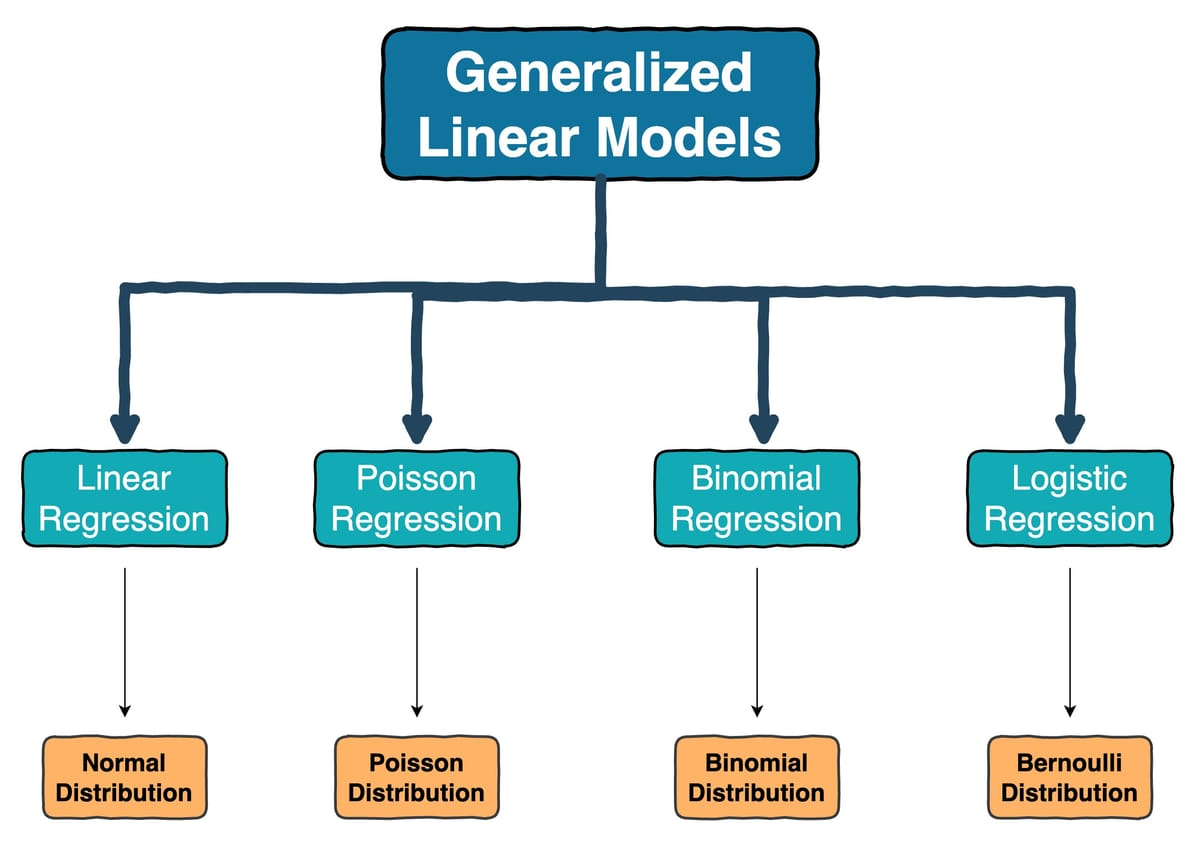
\includegraphics{fig/glm.jpeg}

\textbf{Reading}

\begin{itemize}
\tightlist
\item
  Chapter 3, Wood S. Generalized Additive Models, 2017. Has a nice
  self-contained introduction to generalized linear models.
\item
  Gelman \& Hill. Data Analysis using Regression and
  Multilevel/Hierarchical Models.2006.
\end{itemize}

\hypertarget{overview-1}{%
\subsection*{\texorpdfstring{\textbf{Overview}}{Overview}}\label{overview-1}}
\addcontentsline{toc}{subsection}{\textbf{Overview}}

In this module, you will learn \textbf{generalized linear models
(GLMs)}, a flexible extension of linear regression that allows for
modeling response variables with error distributions other than the
normal distribution.

\textbf{After completing this module, you will be able to:}

\begin{itemize}
\item
  Explain components of GLMs (link functions, linear predictor, and
  error distribution)
\item
  Fit and interpret logistic and Poisson regression models.
\item
  Calculate and interpret odds ratios and rate ratios.
\item
  Perform hypothesis testing using Wald and likelihood ratio tests.
\end{itemize}

\hypertarget{motivation-and-examples-2}{%
\subsection*{Motivation and Examples}\label{motivation-and-examples-2}}
\addcontentsline{toc}{subsection}{Motivation and Examples}

\begin{tcolorbox}[enhanced jigsaw, breakable, colbacktitle=quarto-callout-important-color!10!white, left=2mm, colframe=quarto-callout-important-color-frame, opacityback=0, coltitle=black, colback=white, rightrule=.15mm, title=\textcolor{quarto-callout-important-color}{\faExclamation}\hspace{0.5em}{Motivation:}, titlerule=0mm, opacitybacktitle=0.6, leftrule=.75mm, toprule=.15mm, arc=.35mm, bottomtitle=1mm, toptitle=1mm, bottomrule=.15mm]

If the outcome variable does not follow a normal distribution,
alternative regression methods, such as generalized linear models, are
required.

\begin{itemize}
\tightlist
\item
  \textbf{Bernoulli/Binomial:} Binary outcomes (0/1) or counts of
  successes out of a fixed number of trials.
\item
  \textbf{Poisson data:} Count data representing the number of events
  occurring over a fixed time, area, or rate.
\end{itemize}

Treating these as continuous outcomes can lead to biased estimates,
incorrect standard errors, and invalid inference because the underlying
distributional assumptions of linear regression are violated.

\end{tcolorbox}

\textbf{Motivating Example: Preterm Births Data}

The dataset: a cohort of live births from Georgia born in the year 2001
\(N = (77,340)\).

Variables:

\begin{itemize}
\item
  ptb: indicator for whether a baby from pregnancy \(i\) was born
  preterm (\textless37 weeks).
\item
  age: the mother's age at delivery (centered at age 25).
\item
  male: indicator of the baby's sex (1=male, 0=female)
\item
  tobacco: indicator for mother's tobacco use during pregnancy (1= yes,
  0 = no).
\end{itemize}

Tobacco is treated as the exposure variables. Mothers age is a
covariate.

\begin{Shaded}
\begin{Highlighting}[]
\FunctionTok{load}\NormalTok{(}\StringTok{"/Users/emilypeterson/Library/CloudStorage/OneDrive{-}EmoryUniversity/BIOS 526/BIOS526\_Book/data/PTB.Rdata"}\NormalTok{)}
\FunctionTok{head}\NormalTok{(dat)}
\end{Highlighting}
\end{Shaded}

\begin{verbatim}
        age ptb male tobacco
4849420  30   0    M       0
2320030  23   0    F       0
3512250  23   0    M       0
4132270  23   0    F       0
4307390  32   0    M       0
3630030  29   0    F       0
\end{verbatim}


\includegraphics{Module_2A_GLM_files/figure-pdf/unnamed-chunk-3-1.pdf}

\begin{center}\rule{0.5\linewidth}{0.5pt}\end{center}

\hypertarget{why-not-linear-regression-the-wrong-approach}{%
\subsubsection*{\texorpdfstring{Why Not linear regression?
\ul{\textbf{The wrong
approach}}}{Why Not linear regression? The wrong approach}}\label{why-not-linear-regression-the-wrong-approach}}
\addcontentsline{toc}{subsubsection}{Why Not linear regression?
\ul{\textbf{The wrong approach}}}

Consider the following multiple linear regression model: For
\(i=1, ..., n\).

\[
  y_i = \beta_0 + \sum_{k=1}^K \beta_k x_{ik} + \epsilon_i \qquad e_i \overset{iid}{\sim} N(0, \sigma^2)
\]

This is equivalent to
\(y_i \sim N(\beta_0 + \sum_{k=1}^K \beta_k x_{ik} , \sigma^2)\) where
\(x_{ik}\) is the \(k^{th}\) linear predictor for observation \(i\).

Reminder of the assumptions of the above model:

\begin{itemize}
\tightlist
\item
  The \(\beta's\) are fixed unknown constants.
\item
  \(y\) is a linear function of the covariates.
\item
  The expectation of the errors \(e's\) is zero.
\item
  Only \(\epsilon's\) are random.
\end{itemize}

Therefore, \(y_i\) follows a normal distribution and the
\(E(y_i|x_i) = \beta_0 + \sum_{k=1}^K \beta_k x_{ik}\). The linear
regression part is used to model the \textbf{mean function} of \(y_i\).
The assumptions do not hold for other kinds of data, i.e, binary, count
data, etc.

\begin{center}\rule{0.5\linewidth}{0.5pt}\end{center}

\hypertarget{the-better-approach-generalized-linear-regression}{%
\subsection*{\texorpdfstring{\ul{The Better Approach: Generalized Linear
Regression}}{The Better Approach: Generalized Linear Regression}}\label{the-better-approach-generalized-linear-regression}}
\addcontentsline{toc}{subsection}{\ul{The Better Approach: Generalized
Linear Regression}}

A generalized linear model (GLM) extends the linear regression to other
distributions, where the response variable is generated from a
distribution in the \ul{exponential family.}

GLMs provide this flexibility by extending linear regression to a
broader set of distributions---specifically, those that belong to the
\textbf{exponential family}. The exponential family is mathematically
convenient because it allows for a :

\begin{itemize}
\tightlist
\item
  A natural way to link the mean of the response to the linear
  predictors via a link function.
\item
  Simple expressions for the mean and variance, which are essential for
  estimation and inference.
\item
  Unified estimation procedures (e.g., MLE).
\end{itemize}

A GLM involves three ingredients:

\begin{enumerate}
\def\labelenumi{\arabic{enumi}.}
\item
  A probability distribution in the Exponential Family.
\item
  A linear model \(x_i'\beta\).
\item
  A \ul{link function} \(g()\) and its inverse \(g^{-1}()\) is the link
  that relates the linear model to the expectation, i.e., transforms the
  mean function to meet the linear model assumptions.

  \[
  \begin{align*}
  E(y_i|x_i) & = \mu_i = g^{-1} (x_i\beta)\\
  Var(y_i|x_i) & = V(\mu_i) =V(g^{-1}(x_i\beta))
  \end{align*}
  \]
\item
  Note: Unlike OLS, the basic form of the GLM does not involve a noise
  variance \ul{(no \(\sigma^2\)).}
\end{enumerate}

\begin{center}\rule{0.5\linewidth}{0.5pt}\end{center}

\hypertarget{exponential-family}{%
\section*{Exponential Family}\label{exponential-family}}
\addcontentsline{toc}{section}{Exponential Family}

\markright{Exponential Family}

\begin{tcolorbox}[enhanced jigsaw, rightrule=.15mm, breakable, left=2mm, colframe=quarto-callout-note-color-frame, opacityback=0, leftrule=.75mm, toprule=.15mm, colback=white, arc=.35mm, bottomrule=.15mm]

The basic form for an exponential family density is

\[
f_{\theta} (y) = exp[\{y\theta - b(\theta)\} / a(\phi) + c(y, \phi )]
\]

where \(a, b, c\) are known functions, and \(\phi\) is a known scale
parameter. The ONLY parameter is \(\theta\).

\end{tcolorbox}

In the GLM, \(\theta\) will be a function of \(x_i\beta\).

Examples of distributions in the exponential family include: normal with
known variance (link = identity), Bernoulli (link = logit or probit),
binomial (link = logit or log), gamma, exponential (link = negative
inverse), and others.

The table below summarizes the three most common GLM families side by
side:

\begin{longtable}[]{@{}
  >{\raggedright\arraybackslash}p{(\columnwidth - 6\tabcolsep) * \real{0.2500}}
  >{\raggedright\arraybackslash}p{(\columnwidth - 6\tabcolsep) * \real{0.2500}}
  >{\raggedright\arraybackslash}p{(\columnwidth - 6\tabcolsep) * \real{0.2500}}
  >{\raggedright\arraybackslash}p{(\columnwidth - 6\tabcolsep) * \real{0.2500}}@{}}
\toprule\noalign{}
\begin{minipage}[b]{\linewidth}\raggedright
\end{minipage} & \begin{minipage}[b]{\linewidth}\raggedright
\textbf{Normal}
\end{minipage} & \begin{minipage}[b]{\linewidth}\raggedright
\textbf{Bernoulli/Binomial}
\end{minipage} & \begin{minipage}[b]{\linewidth}\raggedright
\textbf{Poisson}
\end{minipage} \\
\midrule\noalign{}
\endhead
\bottomrule\noalign{}
\endlastfoot
Natural param \(\theta\) & \(\mu\) & \(\log\!\frac{p}{1-p}\) &
\(\log\lambda\) \\
\(b(\theta)\) & \(\theta^2/2\) & \(n\log(1+e^\theta)\) & \(e^\theta\) \\
Canonical link \(g(\mu)\) & identity & logit & log \\
\(E(Y)\) & \(\mu\) & \(np\) & \(\lambda\) \\
\(\text{Var}(Y)\) & \(\sigma^2\) & \(np(1-p)\) & \(\lambda\) \\
Use when & continuous, symmetric & binary / bounded counts & unbounded
counts / rates \\
\end{longtable}

Lets derive a general class for the exponential function. \emph{Use the
expandable panels below to explore key statistical properties and their
derivations.}

\begin{tcolorbox}[enhanced jigsaw, rightrule=.15mm, breakable, left=2mm, colframe=quarto-callout-tip-color-frame, opacityback=0, leftrule=.75mm, toprule=.15mm, colback=white, arc=.35mm, bottomrule=.15mm]

\textbf{The Binomial Distribution}\vspace{2mm}

\begin{enumerate}
\def\labelenumi{\arabic{enumi}.}
\tightlist
\item
  The Binomial distribution with parameters \(n\) and \(p\) is:
\end{enumerate}

\[f(y \mid p) = \binom{n}{y} p^y (1-p)^{n-y},\]

which can be expressed in the exponential family form:

\[f(y \mid \theta) = \exp \left[ y \theta - b(\theta) + c(y) \right], \]
where
\[\theta = \log \left( \frac{p}{1-p} \right), \quad b(\theta) = n \log (1 + e^{\theta}), \quad c(y) = \log \binom{n}{y}. \]

The mean and variance are:
\[ E[Y] = np, \qquad \text{Var}(Y) = np(1-p). \]

\textbf{Why the logit is the canonical link:}
\(\theta = \log\!\frac{p}{1-p}\) falls directly out of matching the
Binomial density to the exponential family form --- it is not a modeling
choice. Verify using \(E(Y) = b'(\theta)\): \[
b'(\theta) = \frac{d}{d\theta}\, n\log(1+e^\theta) = \frac{ne^\theta}{1+e^\theta} = np \ \checkmark
\] and \(\text{Var}(Y) = b''(\theta) \cdot a(\phi)\): \[
b''(\theta) = \frac{ne^\theta}{(1+e^\theta)^2} = np(1-p) \ \checkmark
\]

\end{tcolorbox}

\begin{tcolorbox}[enhanced jigsaw, rightrule=.15mm, breakable, left=2mm, colframe=quarto-callout-tip-color-frame, opacityback=0, leftrule=.75mm, toprule=.15mm, colback=white, arc=.35mm, bottomrule=.15mm]

\textbf{The Poisson Distribution}\vspace{2mm}

The Poisson distribution with parameter \(\lambda > 0\) is:

\[f(y \mid \lambda) = \frac{\lambda^y e^{-\lambda}}{y!}, \]

which can be expressed in the exponential family form:

\[f(y \mid \theta) = \exp \left[ y \theta - b(\theta) + c(y) \right], \]
where
\[\theta = \log (\lambda), \quad b(\theta) = e^{\theta}, \quad c(y) = - \log (y!). \]

The mean and variance are:
\[E[Y] = \lambda, \qquad \text{Var}(Y) = \lambda. \]

\end{tcolorbox}

\begin{tcolorbox}[enhanced jigsaw, rightrule=.15mm, breakable, left=2mm, colframe=quarto-callout-tip-color-frame, opacityback=0, leftrule=.75mm, toprule=.15mm, colback=white, arc=.35mm, bottomrule=.15mm]

\textbf{The Gamma Distribution}\vspace{2mm}

\begin{enumerate}
\def\labelenumi{\arabic{enumi}.}
\setcounter{enumi}{2}
\tightlist
\item
  The Gamma distribution (shape \(k\), scale \(\phi\)) has the density:
\end{enumerate}

\[f(y \mid k, \phi) = \frac{1}{\Gamma(k) \phi^k} y^{k-1} e^{-y/\phi}, \quad y > 0. \]

It can be expressed in the exponential family form:

\[f(y \mid \theta) = \exp \left[ \frac{y \theta - b(\theta)}{a(\phi)} + c(y, \phi) \right], \]
where
\[ \theta = -\frac{1}{k\phi}, \quad b(\theta) = - \log (-\theta), \quad a(\phi) = \frac{1}{k}, \quad c(y, \phi) = (k-1)\log y - \log \Gamma(k). \]

The mean and variance are:
\[E[Y] = k \phi, \qquad \text{Var}(Y) = k \phi^2. \]

\end{tcolorbox}

\begin{center}\rule{0.5\linewidth}{0.5pt}\end{center}

\hypertarget{logistic-regression}{%
\section*{Logistic Regression}\label{logistic-regression}}
\addcontentsline{toc}{section}{Logistic Regression}

\markright{Logistic Regression}

\hypertarget{bernoulli-model}{%
\subsubsection*{Bernoulli Model}\label{bernoulli-model}}
\addcontentsline{toc}{subsubsection}{Bernoulli Model}

Let's take a binary outcome where \(p_i\) is the probability of success.
For \(i=1,...,n\) assume

\[ 
y_i \sim Bernoulli (p_i)
\]

where \(p_i \in (0,1)\) and the Bernoulli function has the following
characteristics:

\[
\begin{align*}
E(y_i) & = p_i\\
Var(y_i) & =V(p_i) = p_i (1- p_i)\\
f(y_i|p_i) & = p_i ^{y_i} (1-p_i)^{1-y_i}
\end{align*}
\]

\begin{center}\rule{0.5\linewidth}{0.5pt}\end{center}

\hypertarget{link-functions}{%
\subsubsection*{Link Functions}\label{link-functions}}
\addcontentsline{toc}{subsubsection}{Link Functions}

We know that \(\mu_i = p_i = P(Y_i=1)\). So we wish to model a
\textbf{link function} \(g()\) that \textbf{enforces a linear
relationship} between the unscaled expectation \(\mu_i\) and the
expectation \(\beta_0 + \sum_{k=1}^K \beta_k x_{ik}\), i.e, we wish to
model

\[
g(\mu_i) = \beta_0 + \sum_{k=1}^K \beta_k x_{ik}
\]

The two most commonly used link functions for binomial data are the
logit and probit functions.

\ul{The \textbf{link function} should have some desirable properties:}

\begin{enumerate}
\def\labelenumi{\arabic{enumi}.}
\tightlist
\item
  \(g()\) should have a range \((-\infty, \infty)\) so that \(\beta's\)
  and \(X's\) can have any value.
\item
  \(g()\) should have a domain that corresponds to all possible values
  of \(\mu_i\), i.e., \((0,1)\) for the binomial distribution.
\item
  \(g()\) should be one-to-one
  \(\mu_i = g^{-1}(\beta_0 + \sum_k \beta_k X_{ik})\).
\item
  \(g()\) should be strictly increasing, i.e.,
  \(g(p_i) \rightarrow \infty\) when \(p_i \rightarrow 1\).
\end{enumerate}

\begin{center}\rule{0.5\linewidth}{0.5pt}\end{center}

\hypertarget{logit-link-logistic-function}{%
\subsubsection*{Logit Link \& Logistic
Function}\label{logit-link-logistic-function}}
\addcontentsline{toc}{subsubsection}{Logit Link \& Logistic Function}

The logit link function is defined as:

\[
g(p_i) = log\left(\frac{p_i}{1-p_i}\right) = \beta_0 + \sum_k \beta_k X_{ik}, \qquad (0,1) \rightarrow (-\infty, \infty)
\]

Meaning \(log(p_i/1-p_i) \rightarrow -\infty\) when
\(p_i \rightarrow 0\) and \(log(p_i/1-p_i)\rightarrow \infty\) when
\(p_i \rightarrow 1\).

In general the logistic function is defined as :

\[
p_i = \frac{e^{g(\mu_i)}}{1 + e^{g(\mu_i)}} = \frac{1}{1+ e^{-g(\mu_i)}}, \qquad (-\infty, \infty) \rightarrow (0,1)
\]

\begin{itemize}
\item
  The \(\beta's\) are estimated using the iterative re-weighted MLE
  method.
\item
  There is no \(\epsilon_i\)!!! Meaning the variance is not defined by a
  normally distributed noise term.
\item
  \(g(p_i)\) is interpreted as the \ul{log\_odds of probability of
  success.}
\end{itemize}

\begin{center}\rule{0.5\linewidth}{0.5pt}\end{center}

\hypertarget{interpretation}{%
\subsubsection*{Interpretation}\label{interpretation}}
\addcontentsline{toc}{subsubsection}{Interpretation}

When \(X_i=0\), \(log(\frac{p_i}{1-p_i}) = \beta_0\) which is
interpreted as the baseline or reference log-odds of probability.

\(\beta_1\) is interpreted as the CHANGE in log-odds per one unit change
in \(X_i\). Conversely, \(e^{\beta_1}\) is defines the odds-ratio.

\[
log(\frac{p_i}{1-p_i}) = \beta_0 + \beta_1 x_i, \text{ versus } log(\frac{p^*_i}{1-p^*_i}) = \beta_0 + \beta_1 (x_i + 1)
\]

then

\[
log\left(\frac{p^*_i/(1-p^*_i)}{p_i/(1-p_i)}\right) = \beta_1
\]

\begin{tcolorbox}[enhanced jigsaw, rightrule=.15mm, breakable, left=2mm, colframe=quarto-callout-note-color-frame, opacityback=0, leftrule=.75mm, toprule=.15mm, colback=white, arc=.35mm, bottomrule=.15mm]

\textbf{Key property:} \(e^{\beta_1}\) does not depend on \(x_i\) ---
the odds ratio is \textbf{constant} across all baseline values of \(X\).
This is the \textbf{proportional odds} property of the logistic model.

\end{tcolorbox}

In the multiple logistic regression, \(\beta_k\) is the log odds ratio
associated with covariate \(k\) while controlling for other covariates.

\begin{center}\rule{0.5\linewidth}{0.5pt}\end{center}

\hypertarget{odds-ratio-indicator-variables}{%
\subsubsection*{Odds Ratio \& Indicator
Variables}\label{odds-ratio-indicator-variables}}
\addcontentsline{toc}{subsubsection}{Odds Ratio \& Indicator Variables}

Odds Ratio interpretation is helpful for indicator variables. Let
\(x_i=1\) in exposed group and \(x_i=0\) in unexposed group. Then:

\[
e^{\beta_1} = \frac{\{\frac{p(y_i=1|x_i=1)}{p(y_i=0|x_i=1)}\}}{\frac{p(y_i=1|x_i=0)}{p(y_i=0|x_i=0)}\}} = \frac{\text{odds(Exposed)}}{\text{odds(Unexposed)}}
\]

\begin{itemize}
\item
  OR\textgreater1 means a positive association
\item
  OR\textless1 means a negative association
\item
  OR=1 means no difference between exposure groups.
\end{itemize}

It is really important to understand that the change in log-odds per one
unit change in \(X_i\) is not constant, i.e, that change in log-odds
depends on the value of \(X_i\).

\begin{Shaded}
\begin{Highlighting}[]
\CommentTok{\#The Logit Function}
\NormalTok{p.i }\OtherTok{\textless{}{-}} \FunctionTok{seq}\NormalTok{(}\DecValTok{0}\NormalTok{, }\DecValTok{1}\NormalTok{, }\AttributeTok{by =} \FloatTok{0.001}\NormalTok{)}
\NormalTok{g\_p.i }\OtherTok{\textless{}{-}} \FunctionTok{log}\NormalTok{(p.i}\SpecialCharTok{/}\NormalTok{(}\DecValTok{1}\SpecialCharTok{{-}}\NormalTok{p.i))}
\FunctionTok{plot}\NormalTok{(p.i, g\_p.i, }\AttributeTok{col =} \StringTok{"red"}\NormalTok{, }\AttributeTok{xlab =}\StringTok{"p"}\NormalTok{, }\AttributeTok{ylab =} \StringTok{"Logit Function"}\NormalTok{)}
\end{Highlighting}
\end{Shaded}

\begin{figure}[H]

{\centering 
\includegraphics{Module_2A_GLM_files/figure-pdf/unnamed-chunk-4-1.pdf}

}

\end{figure}

\begin{Shaded}
\begin{Highlighting}[]
\CommentTok{\#The Logistic Function}
\NormalTok{p\_i }\OtherTok{\textless{}{-}} \FunctionTok{exp}\NormalTok{(g\_p.i)}\SpecialCharTok{/}\NormalTok{(}\DecValTok{1}\SpecialCharTok{+}\FunctionTok{exp}\NormalTok{(g\_p.i))}
\FunctionTok{plot}\NormalTok{(g\_p.i, p\_i, }\AttributeTok{col =} \StringTok{"blue"}\NormalTok{, }\AttributeTok{xlab =} \StringTok{"x"}\NormalTok{, }\AttributeTok{ylab =} \StringTok{"Logistic Function"}\NormalTok{)}
\end{Highlighting}
\end{Shaded}

\begin{figure}[H]

{\centering 
\includegraphics{Module_2A_GLM_files/figure-pdf/unnamed-chunk-4-2.pdf}

}

\end{figure}

What are the effects of changing the baseline odds?

\[
\begin{align}
logit(p_i)& = \beta_0 + x_i\\
\mu_i = P(Y_i =1) &= \frac{e^{\beta_0 + x_i}}{1 + e^{\beta_0 + x_i}}
\end{align}
\]


\includegraphics{Module_2A_GLM_files/figure-pdf/unnamed-chunk-5-1.pdf}

Note: The shape is maintained, and the baseline (intercept) probability
changes.

What are the effects of the change in slope?

\[
\begin{align}
logit(p_i)& = \beta_1 x_i\\
\mu_i = P(Y_i =1) = \frac{e^{\beta_1 x_i}}{1 + e^{\beta_1 x_i}}
\end{align}
\]


\includegraphics{Module_2A_GLM_files/figure-pdf/unnamed-chunk-6-1.pdf}

Note how the steepness changes with difference in slopes. Also note how
the direction changes depending on the effect changes.

\begin{center}\rule{0.5\linewidth}{0.5pt}\end{center}

\hypertarget{fitting-a-logistic-regression-in-r}{%
\subsubsection*{Fitting a logistic regression in
R}\label{fitting-a-logistic-regression-in-r}}
\addcontentsline{toc}{subsubsection}{Fitting a logistic regression in R}

We come back to our motivating example using data on preterm births in
Georgia (2001).

Fitting the GLM model in R is very similar to fitting a linear
regression model. We need to specify the distribution as
\textcolor{blue}{binomial}and the link function as
\textcolor{blue}{logit}.

\begin{Shaded}
\begin{Highlighting}[]
\DocumentationTok{\#\#\# The GLM Function}

\FunctionTok{load}\NormalTok{(}\StringTok{"/Users/emilypeterson/Library/CloudStorage/OneDrive{-}EmoryUniversity/BIOS 526/BIOS526\_Book/data/PTB.Rdata"}\NormalTok{)}

\NormalTok{fit }\OtherTok{\textless{}{-}} \FunctionTok{glm}\NormalTok{(}\AttributeTok{formula =}\NormalTok{ ptb }\SpecialCharTok{\textasciitilde{}}\NormalTok{ age }\SpecialCharTok{+}\NormalTok{ male }\SpecialCharTok{+}\NormalTok{ tobacco, }
    \AttributeTok{family =} \FunctionTok{binomial}\NormalTok{(}\AttributeTok{link =} \StringTok{"logit"}\NormalTok{),}
    \AttributeTok{data =}\NormalTok{ dat)}

\FunctionTok{summary}\NormalTok{(fit)}
\end{Highlighting}
\end{Shaded}

\begin{verbatim}

Call:
glm(formula = ptb ~ age + male + tobacco, family = binomial(link = "logit"), 
    data = dat)

Coefficients:
              Estimate Std. Error z value Pr(>|z|)    
(Intercept) -2.4212664  0.0631355 -38.350  < 2e-16 ***
age         -0.0006295  0.0021596  -0.291  0.77068    
maleM        0.0723659  0.0258672   2.798  0.00515 ** 
tobacco      0.4096495  0.0534627   7.662 1.83e-14 ***
---
Signif. codes:  0 '***' 0.001 '**' 0.01 '*' 0.05 '.' 0.1 ' ' 1

(Dispersion parameter for binomial family taken to be 1)

    Null deviance: 44908  on 77339  degrees of freedom
Residual deviance: 44846  on 77336  degrees of freedom
AIC: 44854

Number of Fisher Scoring iterations: 5
\end{verbatim}

\textbf{Model Interpretation}

\begin{itemize}
\item
  Preterm delivery was significantly associated with male babies
  (p-value = 0.005) when controlling for age and mother's smoking
  status. The \ul{odds ratio} of a preterm birth for a male baby versus
  a female baby was 1.07 (95\% CI: 1.02, 1.13).
\item
  \(OR = e^{0.0723} = 1.07\) with 95\% CI = (1.02, 1.13).

  \begin{itemize}
  \item
    How we get CIs: \(e^{(0.0723 \pm 1.96 * 0.0258)}\).

    NOTE: TRANSFORM THE INTERVALS. DO NOT TRANSFORM THE STANDARD ERRORS
    (this requires the delta method).
  \end{itemize}
\item
  Preterm delivery was significantly associated with whether the mother
  smoked during pregnancy (p\textless0.001) when controlling for age and
  the baby's sex.
\item
  \(OR = e^{0.409} = 1.51 (1.36, 1.67)\).
\item
  The baseline proportion (female babies born to mother of age 25 who
  didn't smoke) of preterm delivery was

  \[
  \frac{e^{-2.42}}{1 + e^{-2.42}} = 0.08.
  \]
\item
  We didn't find an effect of mother's age.
\end{itemize}

\begin{center}\rule{0.5\linewidth}{0.5pt}\end{center}

\hypertarget{wald-test}{%
\subsubsection*{Wald Test}\label{wald-test}}
\addcontentsline{toc}{subsubsection}{Wald Test}

The \textbf{Wald Test} evaluates the significance of individual
regression coefficients directly by comparing the estimated coefficient
to its standard error. The Wald Test relied on the fact that MLEs of the
coefficients are approximately normally distributed for large samples
(Central Limit Theorem).

\begin{tcolorbox}[enhanced jigsaw, rightrule=.15mm, breakable, left=2mm, colframe=quarto-callout-note-color-frame, opacityback=0, leftrule=.75mm, toprule=.15mm, colback=white, arc=.35mm, bottomrule=.15mm]

Wald test under regularity conditions and assuming asymptotic results,

\[
\begin{align}
\hat{\beta} &\sim N(\beta, I(\beta)^{-1})\\
I(\beta) &= E\left\{\left(\frac{\partial l}{\partial \beta}\right)\left(\frac{\partial l}{\partial \beta}\right)'\right\}\\
&= -E\frac{\partial^2 l}{\partial \beta \partial \beta'}
\end{align}
\]

\begin{itemize}
\item
  \(I(\beta)\) is called the Fisher information matrix (see Wood p.106).
  The standard error of \(\hat{\beta}\) is derived from
  \(I(\beta)^{-1}\).
\item
  The Wald test uses the standardized statistic: \[
  Z = \frac{\hat{\beta}_i}{s.e.(\hat{\beta}_i)}
  \]
\end{itemize}

\end{tcolorbox}

\begin{itemize}
\item
  The \(Z-\) column is calculated as
  \(z = \frac{\hat{\beta}_i}{SE(\hat{\beta}_i)}\).
\item
  The p-values are derived from the z-statistic \(H_0 : \beta_i = 0\).
  For example, for \textt{male}, \(z \approx 2.798\) with \(p=0.005\)
  indicating male babies are significantly associated with preterm birth
  holding other variables constant.
\end{itemize}

\begin{center}\rule{0.5\linewidth}{0.5pt}\end{center}

\hypertarget{likelihood-ratio-test}{%
\subsubsection*{Likelihood Ratio Test}\label{likelihood-ratio-test}}
\addcontentsline{toc}{subsubsection}{Likelihood Ratio Test}

In logistic regression, we use the Likelihood Ratio Test to determine
whether adding predictors significantly improves model fit, since
standard F-tests from linear regression do not apply. The Likelihood
Ratio Test (LRT) provides a natural way to compare nested models by
examining how much better the full model fits the data compared to a
reduced model (with some parameters set to zero):
\textcolor{blue}{How can we test whether which model is better?}

The likelihood ratio test (LRT) is used to test the null hypothesis that
any subset of the \(\beta's\) is equal to 0. The number of \(\beta's\)
in the full model is \(k+1\), while the number of \(\beta's\) in the
reduced model is \(r+1\). (Remember the reduced model is the model that
results when the \(\beta's\) in the null hypothesis are set to 0). Thus,
the number of \(\beta's\) being tested in the null hypothesis is
\((k+1) - (r+1) = k-r\).

\begin{tcolorbox}[enhanced jigsaw, rightrule=.15mm, breakable, left=2mm, colframe=quarto-callout-note-color-frame, opacityback=0, leftrule=.75mm, toprule=.15mm, colback=white, arc=.35mm, bottomrule=.15mm]

The Likelihood Ratio Test is given by:

\[
LR= \frac{max_{H_0}L(\beta)}{max_{H_A}L(\beta)}
\] This gives the ratio of the likelihood of the null model evaluated at
the MLEs to the likelihood of the full model evaluated at the MLEs.

\begin{itemize}
\tightlist
\item
  In the normal case, this is the analogous to the F-test described in
  Chapter 1.
\end{itemize}

The likelihood ratio test statistic is given by:

\[
\lambda_{LR} = -2[l(\hat{\beta}_{reduced}) - l(\hat{\beta}_{full})]
\]

\begin{itemize}
\item
  The difference follows a Chi-square distribution, i.e.,

  \[
  \lambda_{LR} > \chi^2_{\nu, 1-\alpha}
  \]
\end{itemize}

where \(\nu\) denotes the different in number of parameters, i.e.,
\(k-r\) = degrees of freedom.

\end{tcolorbox}

The likelihood for a binary logistic regression is given by:

\[
L(\beta; \mathbf{y}, \mathbf{X}) = \prod_{i=1}^{n} \pi_i^{y_i} (1-\pi_i)^{1-y_i}
\]

This yields a log-likelihood of:

\[
\begin{align*}
l(\beta) &= \sum_{i=1}^n [y_i log(\pi_i)  + (1-y_i) log(1-\pi_i)\\
&= \sum_{i=1}^n [y_i \mathbf{X}_i \beta - log(1+ exp(\mathbf{X}_i \beta))]
\end{align*}
\]

Maximizing the LL has \ul{no closed form solution}, so a technique used
to obtain MLEs \(\hat{\beta}\) is iteratively reweighted least squares
(not covered here).

\begin{Shaded}
\begin{Highlighting}[]
\FunctionTok{library}\NormalTok{(car)}
\end{Highlighting}
\end{Shaded}

\begin{verbatim}
Loading required package: carData
\end{verbatim}

\begin{verbatim}

Attaching package: 'car'
\end{verbatim}

\begin{verbatim}
The following object is masked from 'package:dplyr':

    recode
\end{verbatim}

\begin{Shaded}
\begin{Highlighting}[]
\FunctionTok{Anova}\NormalTok{(fit)}
\end{Highlighting}
\end{Shaded}

\begin{verbatim}
Analysis of Deviance Table (Type II tests)

Response: ptb
        LR Chisq Df Pr(>Chisq)    
age        0.085  1   0.770669    
male       7.834  1   0.005126 ** 
tobacco   53.648  1  2.399e-13 ***
---
Signif. codes:  0 '***' 0.001 '**' 0.01 '*' 0.05 '.' 0.1 ' ' 1
\end{verbatim}

\textbf{Interpretation}

\begin{itemize}
\item
  Comparing the full vs reduced model with everything EXCEPT age, we see
  a \(\chi^2\) statistic of 0.085 with a p-value of 0.77 meaning that
  removing age does not significantly worsen the model fit, i.e., age is
  not a significant predictor when controlling for other variables.
\item
  Removing the male variable significantly worsens model fit \(p<0.01\),
  meaning this is a significant predictor.
\item
  Tobacco use has a \(\chi^2\) statistic of 53.65 and a p-value of
  \textless0.001, meaning it is a highly significant predictor, and
  removing it significantly reduces model fit.
\end{itemize}

\begin{center}\rule{0.5\linewidth}{0.5pt}\end{center}

\hypertarget{wald-vs.-lrt-when-to-use-which}{%
\subsubsection*{Wald vs.~LRT: When to Use
Which}\label{wald-vs.-lrt-when-to-use-which}}
\addcontentsline{toc}{subsubsection}{Wald vs.~LRT: When to Use Which}

\begin{longtable}[]{@{}
  >{\raggedright\arraybackslash}p{(\columnwidth - 4\tabcolsep) * \real{0.3333}}
  >{\raggedright\arraybackslash}p{(\columnwidth - 4\tabcolsep) * \real{0.3333}}
  >{\raggedright\arraybackslash}p{(\columnwidth - 4\tabcolsep) * \real{0.3333}}@{}}
\toprule\noalign{}
\begin{minipage}[b]{\linewidth}\raggedright
\end{minipage} & \begin{minipage}[b]{\linewidth}\raggedright
\textbf{Wald Test}
\end{minipage} & \begin{minipage}[b]{\linewidth}\raggedright
\textbf{Likelihood Ratio Test}
\end{minipage} \\
\midrule\noalign{}
\endhead
\bottomrule\noalign{}
\endlastfoot
Statistic & \(Z = \hat{\beta}_j / \text{SE}(\hat{\beta}_j)\) &
\(\lambda_{LR} = -2[l_{\text{reduced}} - l_{\text{full}}]\) \\
Distribution & \(N(0,1)\) & \(\chi^2_{k-r}\) \\
Best for & Single coefficient & Nested model comparison \\
Requires & Large \(n\) (asymptotics) & Same data, same likelihood
type \\
More reliable in small \(n\)? & No & Yes \\
In R & \texttt{summary(fit)} & \texttt{anova(...,\ test="LRT")} or
\texttt{car::Anova(fit)} \\
\end{longtable}

\begin{center}\rule{0.5\linewidth}{0.5pt}\end{center}

\hypertarget{section-7}{%
\section*{\texorpdfstring{\textcolor{purple}{Summary}}{}}\label{section-7}}
\addcontentsline{toc}{section}{\textcolor{purple}{Summary}}

\markright{\textcolor{purple}{Summary}}

\begin{longtable}[]{@{}
  >{\raggedright\arraybackslash}p{(\columnwidth - 2\tabcolsep) * \real{0.2222}}
  >{\raggedright\arraybackslash}p{(\columnwidth - 2\tabcolsep) * \real{0.7778}}@{}}
\toprule\noalign{}
\begin{minipage}[b]{\linewidth}\raggedright
\textbf{Section}
\end{minipage} & \begin{minipage}[b]{\linewidth}\raggedright
\textbf{Description}
\end{minipage} \\
\midrule\noalign{}
\endhead
\bottomrule\noalign{}
\endlastfoot
\textbf{What is the model?} & A \textbf{generalized linear model (GLM)}
links the expected response \(E(Y|X) = \mu\) to predictors via a link
function: \(g(\mu) = \beta_0 + \sum_k \beta_k x_{ik}\). The response
\(Y\) must follow a distribution in the \textbf{exponential family}
(e.g., Normal, Bernoulli, Binomial). \\
\textbf{Model Components} & \textbf{1. Random component:} Distribution
of \(Y\) (e.g., Bernoulli for binary data). \textbf{2. Systematic
component:} Linear predictor \(\eta_i = x_i' \beta\). \textbf{3. Link
function:} \(g(\mu_i)\) maps mean response to \(\eta_i\). \\
\textbf{Logistic Regression} & Special case of GLM for \textbf{binary
outcomes} (\(Y \in \{0,1\}\)) using the logit link:
\(g(p) = \log \frac{p}{1-p}\). Coefficients \(\beta_j\) represent
changes in \textbf{log-odds}, while \(e^{\beta_j}\) are \textbf{odds
ratios}. \\
\textbf{Model Assumptions} & - Correct link function (e.g., logit). -
Independent observations. - Mean and variance correctly specified for
Bernoulli data: \(E(Y)=p\), \(Var(Y)=p(1-p)\). \\
\textbf{Hypothesis Testing} & \textbf{Wald Test:} Tests
\(H_0: \beta_j = 0\) using
\(Z = \hat{\beta}_j / \text{SE}(\hat{\beta}_j)\). \textbf{Likelihood
Ratio Test (LRT):} Compares nested models with
\(\lambda_{LR} = -2 [l_{reduced} - l_{full}] \sim \chi^2\). \\
\textbf{Interpretation} & - \(\beta_j\): Change in log-odds of success
for a one-unit increase in \(X_j\), holding other variables constant. -
\(e^{\beta_j}\): Odds ratio (OR) for a one-unit change in \(X_j\). -
Intercept \(\beta_0\): Baseline log-odds for reference group. \\
\end{longtable}

\bookmarksetup{startatroot}

\hypertarget{module-2b-generalized-linear-models}{%
\chapter*{Module 2B Generalized Linear
Models}\label{module-2b-generalized-linear-models}}
\addcontentsline{toc}{chapter}{Module 2B Generalized Linear Models}

\markboth{Module 2B Generalized Linear Models}{Module 2B Generalized
Linear Models}

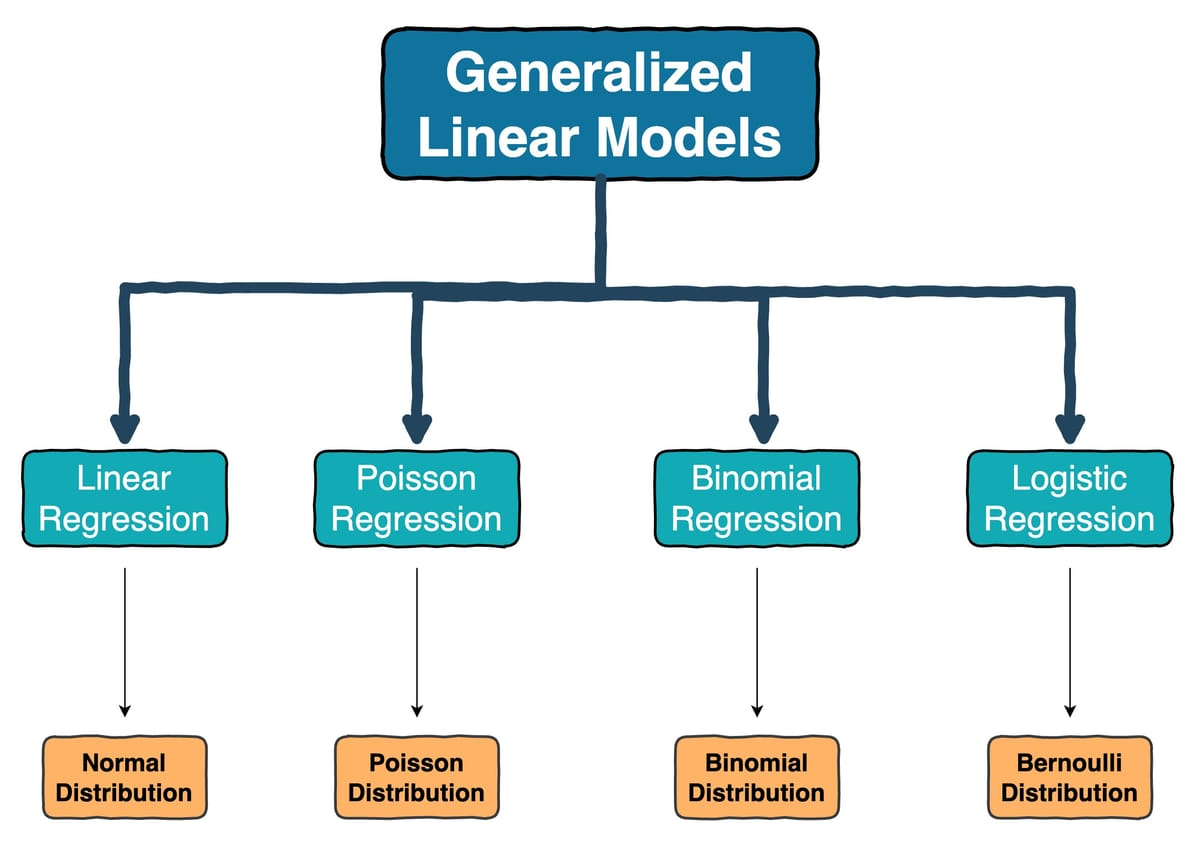
\includegraphics{fig/glm.jpeg}

\hypertarget{poisson-regression}{%
\section*{Poisson Regression}\label{poisson-regression}}
\addcontentsline{toc}{section}{Poisson Regression}

\markright{Poisson Regression}

The Poisson model is used for count data, that is; where each data point
\(y_i\) can equal 0,1,2,\ldots.N. Poisson models are commonly used for
assessing disease and/or mortality counts particularly for rare
diseases.

\begin{center}\rule{0.5\linewidth}{0.5pt}\end{center}

\hypertarget{model-setup}{%
\subsubsection*{Model Setup}\label{model-setup}}
\addcontentsline{toc}{subsubsection}{Model Setup}

We assume that \(y_i\) follows a Poisson distribution: \[
y_i \sim Poisson(\theta_i) = \frac{e^{-\theta_i}\theta_i^{y_i}}{y_i !}
\]

where \(\theta_i>0\) is the expected count for observation \(i\).

\begin{itemize}
\tightlist
\item
  An important characteristic of the Poisson distribution is that the
  mean and variance are equal:
\end{itemize}

\[
E(y_i ) = Var(y_i) = \theta_i
\] - This is notable because it is a characteristic that determines
whether Poisson is an appropriate model assumption.

\begin{itemize}
\tightlist
\item
  As with linear and logistic regression, the variation in \(y\) can be
  explained with linear predictors \(X\).
\end{itemize}

\[
\theta_i = exp(X_i \beta)
\]

\begin{itemize}
\tightlist
\item
  Here the \ul{link} is the log() link. log() has domain \((0, \infty)\)
  and range \((-\infty, \infty)\) and is strictly increasing.
\end{itemize}

\[
g(\theta_i) = log(\theta_i)
\] which maps \((0, \infty) \to (-\infty, \infty)\).

\begin{center}\rule{0.5\linewidth}{0.5pt}\end{center}

\hypertarget{interpretation-of-coefficients}{%
\subsubsection*{Interpretation of
Coefficients}\label{interpretation-of-coefficients}}
\addcontentsline{toc}{subsubsection}{Interpretation of Coefficients}

\begin{itemize}
\tightlist
\item
  Consider a simple Poisson regression model with only one covariate:
\end{itemize}

\[
\begin{align*}
y_i &\overset{ind}{\sim} Pois(\theta_i)\\
log(\theta_i) & = \beta_0 + \beta_1 x_i
\end{align*}
\]

\begin{itemize}
\item
  The coefficient \(\beta_j\) represents the \textbf{log change} in the
  expected count for a one-unit increase in \(X_j\) holding other
  predictors constant.
\item
  Exponentiating \(\beta_j\) gives the \textbf{incidence rate ratio
  (IRR)}:
\end{itemize}

\[
exp(\beta_j) = \frac{\theta_i^*}{\theta_i}
\]

How did we get that?

\textbf{Baseline scenario:} \((X_{ij} = x)\), with expected count
\((\theta_i )\).

\textbf{One-unit increase in} \((X_{ij})\): \((X_{ij} = x + 1)\), with
expected count \((\theta_i^{*} )\).

The difference in log-mean is:

\[
\log \theta_i^{*} - \log \theta_i = \beta_j.
\] Exponentiating both sides, we have:

\[
e^{\beta_j} = \frac{\theta_i^{*}}{\theta_i},
\]

which is interpreted as the \textbf{incidence rate ratio (IRR)} --- the
multiplicative change in the expected count for a one-unit increase in
\(( X_{ij} )\), holding other variables constant.

\begin{center}\rule{0.5\linewidth}{0.5pt}\end{center}

\hypertarget{fitting-a-poisson-regression-in-r}{%
\subsubsection*{Fitting a Poisson Regression in
R}\label{fitting-a-poisson-regression-in-r}}
\addcontentsline{toc}{subsubsection}{Fitting a Poisson Regression in R}

We are going to use the preterm birth data from Georgia to illustrate
our approach. For this analysis, the data have been aggregated by 5-year
maternal age groups and stratified by infant sex and maternal tobacco
use. This aggregation allows us to model counts of preterm births
(events) relative to the number of total live births (exposure) using a
Poisson regression.

\begin{Shaded}
\begin{Highlighting}[]
\FunctionTok{library}\NormalTok{(lme4)}
\FunctionTok{library}\NormalTok{(lmerTest)}
\FunctionTok{library}\NormalTok{(dplyr)}

\FunctionTok{load}\NormalTok{(}\StringTok{"/Users/emilypeterson/Library/CloudStorage/OneDrive{-}EmoryUniversity/BIOS 526/BIOS526\_Book/data/PTB.Rdata"}\NormalTok{)}


\NormalTok{dat}\SpecialCharTok{$}\NormalTok{age\_group }\OtherTok{\textless{}{-}} \FunctionTok{cut}\NormalTok{(dat}\SpecialCharTok{$}\NormalTok{age,}
                     \AttributeTok{breaks =} \FunctionTok{seq}\NormalTok{(}\DecValTok{15}\NormalTok{, }\DecValTok{45}\NormalTok{, }\DecValTok{5}\NormalTok{),}
                     \AttributeTok{right =} \ConstantTok{FALSE}\NormalTok{,}
                     \AttributeTok{labels =} \FunctionTok{c}\NormalTok{(}\StringTok{"15{-}19"}\NormalTok{, }\StringTok{"20{-}24"}\NormalTok{, }\StringTok{"25{-}29"}\NormalTok{, }\StringTok{"30{-}34"}\NormalTok{, }\StringTok{"35{-}39"}\NormalTok{, }\StringTok{"40{-}44"}\NormalTok{))}

\NormalTok{agg\_data }\OtherTok{\textless{}{-}}\NormalTok{ dat }\SpecialCharTok{\%\textgreater{}\%}
  \FunctionTok{group\_by}\NormalTok{(age\_group, male, tobacco) }\SpecialCharTok{\%\textgreater{}\%}
  \FunctionTok{summarise}\NormalTok{(}
    \AttributeTok{events =} \FunctionTok{sum}\NormalTok{(ptb),}
    \AttributeTok{total =} \FunctionTok{n}\NormalTok{()}
\NormalTok{  )}

\FunctionTok{head}\NormalTok{(agg\_data)}
\end{Highlighting}
\end{Shaded}

\begin{verbatim}
# A tibble: 6 x 5
# Groups:   age_group, male [3]
  age_group male  tobacco events total
  <fct>     <fct>   <int>  <int> <int>
1 15-19     F           0    315  3184
2 15-19     F           1     31   245
3 15-19     M           0    325  3297
4 15-19     M           1     26   276
5 20-24     F           0    696  8257
6 20-24     F           1     61   663
\end{verbatim}

Here we can see the \textbf{number of preterm births (\texttt{events})
for each age-group--sex--tobacco combination}, as well as the
\textbf{total number of live births (\texttt{total})} in that subgroup.

To fit a Poisson regression, we model the counts of events with a
\textbf{log link function}, using the total number of births as an
\textbf{offset}:

\begin{Shaded}
\begin{Highlighting}[]
\NormalTok{fit\_poisson }\OtherTok{\textless{}{-}} \FunctionTok{glm}\NormalTok{(events }\SpecialCharTok{\textasciitilde{}}\NormalTok{ age\_group }\SpecialCharTok{+}\NormalTok{ male }\SpecialCharTok{+}\NormalTok{ tobacco,}
                   \AttributeTok{family =}\NormalTok{ poisson,}
                   \AttributeTok{offset =} \FunctionTok{log}\NormalTok{(total),}
                   \AttributeTok{data =}\NormalTok{ agg\_data)}

\FunctionTok{summary}\NormalTok{(fit\_poisson)}
\end{Highlighting}
\end{Shaded}

\begin{verbatim}

Call:
glm(formula = events ~ age_group + male + tobacco, family = poisson, 
    data = agg_data, offset = log(total))

Coefficients:
               Estimate Std. Error z value Pr(>|z|)    
(Intercept)    -2.37223    0.04040 -58.713  < 2e-16 ***
age_group20-24 -0.11935    0.04533  -2.633  0.00847 ** 
age_group25-29 -0.24692    0.04539  -5.441 5.31e-08 ***
age_group30-34 -0.21900    0.04570  -4.792 1.65e-06 ***
age_group35-39 -0.04205    0.05075  -0.829  0.40736    
age_group40-44  0.12036    0.08087   1.488  0.13668    
maleM           0.06634    0.02474   2.682  0.00733 ** 
tobacco         0.34917    0.05029   6.943 3.83e-12 ***
---
Signif. codes:  0 '***' 0.001 '**' 0.01 '*' 0.05 '.' 0.1 ' ' 1

(Dispersion parameter for poisson family taken to be 1)

    Null deviance: 148.530  on 23  degrees of freedom
Residual deviance:  29.892  on 16  degrees of freedom
AIC: 202.82

Number of Fisher Scoring iterations: 4
\end{verbatim}

\textbf{Model Interpretation:}

\begin{itemize}
\item
  The intercept (\(\hat{\beta}_0 = -2.37\)) represents the log rate of
  preterm birth for the reference group: mothers aged 15--19, with
  female infants and no tobacco use. Converting to a rate:
  \(e^{-2.37} \approx 0.093\), meaning about 9 preterm births per 100
  live births in this reference group.
\item
  Age effects: Compared to mothers aged 15--19: Ages 20--24 have a 11\%
  lower rate of preterm birth: \(e^{-0.119} \approx 0.89\) (p = 0.008).
  Ages 25--29 have a 22\% lower rate: \(e^{-0.247} \approx 0.78\) (p
  \textless{} 0.001). Ages 30--34 have a 20\% lower rate:
  \(e^{-0.219} \approx 0.80\) (p \textless{} 0.001). No significant
  difference is observed for ages 35--39 or 40--44 (p \textgreater{}
  0.05).
\item
  Infant sex: Male infants have a 6.9\% higher preterm birth rate
  compared to female infants: \(e^{0.066} \approx 1.07\) (p = 0.007).
\item
  Tobacco use: Mothers who smoke have a 42\% higher preterm birth rate
  compared to non-smokers: \(e^{0.349} \approx 1.42\) (p \textless{}
  0.001).
\item
  Goodness-of-fit: The residual deviance (29.89 on 16 df) suggests an
  adequate fit, and the model explains a substantial portion of
  variation compared to the null model (null deviance = 148.53).
\end{itemize}

\begin{center}\rule{0.5\linewidth}{0.5pt}\end{center}

\hypertarget{what-is-an-offset}{%
\subsubsection*{What is an Offset?}\label{what-is-an-offset}}
\addcontentsline{toc}{subsubsection}{What is an Offset?}

In the code above you saw a parameter in the glm
\(\text{offset = log(total)}\). This is called an offset in Poisson
regression.

When modeling \textbf{rates} rather than raw counts, it is critical to
account for the \textbf{population-at-risk} or the \textbf{exposure
time} for each observation. In the context of preterm birth data, the
\textbf{total number of live births} within each age--sex--tobacco
subgroup serves as the population-at-risk. Without this adjustment,
groups with larger populations would naturally have higher counts simply
due to their size, not because they have a higher risk of preterm
births.

\textbf{Why Use an Offset?}

\begin{itemize}
\item
  The Poisson regression models the expected \textbf{count} of events
  \(y_i\) as: \[
  y_i \sim \text{Poisson}(\theta_i)
  \] where \(\theta_i\) is the \textbf{expected count} for the \(i\)th
  subgroup.
\item
  To model \textbf{rates}, we can express: \[
  \text{Rate}_i = \frac{\theta_i}{N_i}
  \] where \(N_i\) is the \textbf{population size} (e.g., total births
  in the subgroup).
\item
  Taking logs: \[
  \log(\theta_i) = \log(N_i) + \log(\text{Rate}_i).
  \] Here, \(\log(N_i)\) is treated as a \textbf{known constant} rather
  than a parameter to estimate.
\item
  This motivates the use of an \textbf{offset term}: \[
  \log(\theta_i) = \log(N_i) + X_i \beta,
  \].
\end{itemize}

\begin{center}\rule{0.5\linewidth}{0.5pt}\end{center}

\hypertarget{poisson-overdispersion}{%
\subsection*{Poisson Overdispersion}\label{poisson-overdispersion}}
\addcontentsline{toc}{subsection}{Poisson Overdispersion}

One of the most important assumptions of the Poisson model is
\textbf{equidispersion}, meaning the variance of the outcome equals the
mean:

\[
E(y_i) = Var(y_i) = \theta_i.
\]

In real data, especially with health outcomes, this assumption often
fails. \textbf{Overdispersion} occurs when the variance is larger than
the mean:

\[
Var(y_i) > E(y_i).
\]

This can lead to: - Standard errors that are too small\\
- Confidence intervals that are too narrow\\
- p-values that are too optimistic

\begin{center}\rule{0.5\linewidth}{0.5pt}\end{center}

\hypertarget{how-to-check-for-overdispersion}{%
\subsubsection*{How to Check for
Overdispersion}\label{how-to-check-for-overdispersion}}
\addcontentsline{toc}{subsubsection}{How to Check for Overdispersion}

A common diagnostic is the \textbf{dispersion statistic}, defined as:

\[
\hat{\phi} = \frac{\text{Residual Deviance}}{\text{Residual Degrees of Freedom}}
\]

\begin{itemize}
\tightlist
\item
  If \(\hat{\phi} \approx 1\), the equidispersion assumption holds.\\
\item
  If \(\hat{\phi} > 1.5\), the data are likely overdispersed.\\
\item
  If \(\hat{\phi} < 1\), underdispersion may be present (less common).
\end{itemize}

In R:

\begin{Shaded}
\begin{Highlighting}[]
\CommentTok{\# Calculate dispersion statistic}
\FunctionTok{deviance}\NormalTok{(fit\_poisson) }\SpecialCharTok{/} \FunctionTok{df.residual}\NormalTok{(fit\_poisson)}
\end{Highlighting}
\end{Shaded}

\begin{verbatim}
[1] 1.868255
\end{verbatim}

\begin{center}\rule{0.5\linewidth}{0.5pt}\end{center}

\hypertarget{remedies-for-overdispersion}{%
\subsubsection*{Remedies for
Overdispersion}\label{remedies-for-overdispersion}}
\addcontentsline{toc}{subsubsection}{Remedies for Overdispersion}

\textbf{Quasi-Poisson Model:}

The quasi-Poisson approach allows the variance to be proportional to the
mean but inflated by a dispersion parameter:

\[
Var(y_i) = \phi \cdot \theta_i
\]

\begin{itemize}
\tightlist
\item
  Implemented in R with \texttt{family\ =\ quasipoisson}.\\
\item
  Coefficient estimates remain the same as Poisson, but \textbf{standard
  errors are corrected}.
\end{itemize}

\begin{Shaded}
\begin{Highlighting}[]
\NormalTok{fit\_quasi }\OtherTok{\textless{}{-}} \FunctionTok{glm}\NormalTok{(events }\SpecialCharTok{\textasciitilde{}}\NormalTok{ age\_group }\SpecialCharTok{+}\NormalTok{ male }\SpecialCharTok{+}\NormalTok{ tobacco,}
                 \AttributeTok{family =}\NormalTok{ quasipoisson,}
                 \AttributeTok{offset =} \FunctionTok{log}\NormalTok{(total),}
                 \AttributeTok{data =}\NormalTok{ agg\_data)}
\FunctionTok{summary}\NormalTok{(fit\_quasi)}
\end{Highlighting}
\end{Shaded}

\begin{verbatim}

Call:
glm(formula = events ~ age_group + male + tobacco, family = quasipoisson, 
    data = agg_data, offset = log(total))

Coefficients:
               Estimate Std. Error t value Pr(>|t|)    
(Intercept)    -2.37223    0.05722 -41.459  < 2e-16 ***
age_group20-24 -0.11935    0.06420  -1.859 0.081512 .  
age_group25-29 -0.24692    0.06427  -3.842 0.001440 ** 
age_group30-34 -0.21900    0.06472  -3.384 0.003788 ** 
age_group35-39 -0.04205    0.07187  -0.585 0.566663    
age_group40-44  0.12036    0.11453   1.051 0.308915    
maleM           0.06634    0.03504   1.894 0.076508 .  
tobacco         0.34917    0.07122   4.903 0.000159 ***
---
Signif. codes:  0 '***' 0.001 '**' 0.01 '*' 0.05 '.' 0.1 ' ' 1

(Dispersion parameter for quasipoisson family taken to be 2.005549)

    Null deviance: 148.530  on 23  degrees of freedom
Residual deviance:  29.892  on 16  degrees of freedom
AIC: NA

Number of Fisher Scoring iterations: 4
\end{verbatim}

\begin{center}\rule{0.5\linewidth}{0.5pt}\end{center}

\hypertarget{differences-between-the-binomial-and-poisson-models}{%
\subsubsection*{Differences between the Binomial and Poisson
models}\label{differences-between-the-binomial-and-poisson-models}}
\addcontentsline{toc}{subsubsection}{Differences between the Binomial
and Poisson models}

The Poisson model is similar to the binomial model for count data but is
applied in slightly different situations.

\begin{itemize}
\item
  If each data point \(y_i\) can be interpreted as the number of
  ``successes'' out of \(n_i\) trials then it is standard to use the
  binomial/logistic model.
\item
  If each data point \(y_i\) does not have a natural limit- it is not
  based on a number of independent trials- then it is standard to use
  the Poisson/log repression model.
\end{itemize}

\begin{center}\rule{0.5\linewidth}{0.5pt}\end{center}

\hypertarget{section-8}{%
\section*{\texorpdfstring{\textcolor{purple}{Summary}}{}}\label{section-8}}
\addcontentsline{toc}{section}{\textcolor{purple}{Summary}}

\markright{\textcolor{purple}{Summary}}

\begin{longtable}[]{@{}
  >{\raggedright\arraybackslash}p{(\columnwidth - 2\tabcolsep) * \real{0.0965}}
  >{\raggedright\arraybackslash}p{(\columnwidth - 2\tabcolsep) * \real{0.9035}}@{}}
\toprule\noalign{}
\begin{minipage}[b]{\linewidth}\raggedright
\textbf{Section}
\end{minipage} & \begin{minipage}[b]{\linewidth}\raggedright
\textbf{Description}
\end{minipage} \\
\midrule\noalign{}
\endhead
\bottomrule\noalign{}
\endlastfoot
\textbf{What is the model?} & \textbf{Poisson Regression:} Models count
data (\(y_i = 0,1,2,...\)) assuming
\(y_i \sim \text{Poisson}(\theta_i)\), where \(E(y_i) = \theta_i\) and
\(Var(y_i) = \theta_i\). The mean count is linked to predictors by
\(\log(\theta_i) = X_i \beta\). \\
\textbf{Link Function} & Uses the \textbf{log link},
\(g(\theta_i) = \log(\theta_i)\), mapping
\((0, \infty) \rightarrow (-\infty, \infty)\). Coefficients represent
changes in the log of the expected count. \\
\textbf{Interpretation} & \(e^{\beta_j}\) is the \textbf{incidence rate
ratio (IRR)}: the multiplicative change in the expected count for a
one-unit increase in \(X_j\), holding other variables constant. \\
\textbf{Offsets} & Adjusts for \textbf{population-at-risk} or exposure
time. The model becomes \(\log(\theta_i) = \log(N_i) + X_i \beta\),
where \(\log(N_i)\) is an offset term (not estimated). \\
\textbf{Model Assumptions} & - Counts are independent. - Mean equals
variance (no overdispersion). - Correct link function (log). \\
\textbf{Overdispersion} & Check using \textbf{dispersion statistic}
(\(\hat{\phi} = \tfrac{\text{Residual Deviance}}{\text{df}}\)). If
\(\hat{\phi} > 1\), use: - \textbf{Quasi-Poisson} (adjusts SEs). -
\textbf{Negative Binomial} (flexible variance). \\
\textbf{Key Differences} & - Use \textbf{Binomial/Logistic} regression
when counts are bounded by a number of trials (\(n_i\)). - Use
\textbf{Poisson} regression when counts have no natural upper limit and
represent rates or events over a fixed exposure. \\
\textbf{Example Findings} & Tobacco use increases preterm birth rate by
\textbf{42\%} (\(IRR \approx 1.42\)), while mothers aged 25--29 have a
\textbf{22\% lower} rate (\(IRR \approx 0.78\)) compared to ages
15--19. \\
\end{longtable}

\bookmarksetup{startatroot}

\hypertarget{module-2c-generalized-linear-mixed-models}{%
\chapter*{Module 2C Generalized Linear Mixed
Models}\label{module-2c-generalized-linear-mixed-models}}
\addcontentsline{toc}{chapter}{Module 2C Generalized Linear Mixed
Models}

\markboth{Module 2C Generalized Linear Mixed Models}{Module 2C
Generalized Linear Mixed Models}

\hypertarget{motivation-and-examples-3}{%
\subsection*{Motivation and Examples}\label{motivation-and-examples-3}}
\addcontentsline{toc}{subsection}{Motivation and Examples}

\begin{tcolorbox}[enhanced jigsaw, breakable, colbacktitle=quarto-callout-important-color!10!white, left=2mm, colframe=quarto-callout-important-color-frame, opacityback=0, coltitle=black, colback=white, rightrule=.15mm, title=\textcolor{quarto-callout-important-color}{\faExclamation}\hspace{0.5em}{Motivation:}, titlerule=0mm, opacitybacktitle=0.6, leftrule=.75mm, toprule=.15mm, arc=.35mm, bottomtitle=1mm, toptitle=1mm, bottomrule=.15mm]

In many real-world datasets, observations are \textbf{non-normal} and
\textbf{not independent}. For example:

\begin{itemize}
\tightlist
\item
  Repeated measurements on the same subject.
\item
  Clusters of data within counties, hospitals, or schools.
\item
  Panel data where observations are grouped by time or region.
\end{itemize}

\textbf{Why can't we use standard GLMs?}

\begin{itemize}
\item
  A standard GLM assumes independent observations. When data are
  clustered, this assumption is violated, leading to \textbf{biased
  standard errors} and \textbf{incorrect inference}.
\item
  To address this, \textbf{Generalized Linear Mixed Models (GLMMs)}
  extend GLMs by including \textbf{random effects} that account for
  within-group correlation and unobserved heterogeneity.
\item
  Essentially we are combining methods learned in Modules 1 and 2.
\end{itemize}

\end{tcolorbox}

\hypertarget{motivating-example-crossover-design}{%
\subsection*{Motivating Example: Crossover
Design}\label{motivating-example-crossover-design}}
\addcontentsline{toc}{subsection}{Motivating Example: Crossover Design}

We consider a crossover trial on cerebrovascular deficiency:

Data were obtained from a crossover trial on the disease of
cerebrovascular deficiency. The goal is to investigate the side effects
of a treatment drug compared to a placebo

Design:

\begin{itemize}
\item
  34 patients: an active drug (A) and followed by placebo (B).
\item
  33 patients: a placebo (B) followed by an active drug (A).
\item
  Outcome: a normal (0) or abnormal (1) electrodiagram.
\item
  Each patient has a binary observation at period 1 and period 2.
\item
  Crossover design: can have ``carryover'' effects which confound
  treatment effect estimation. Test whether washout period was adequate.
\end{itemize}

Variables:

\begin{itemize}
\item
  ID \(i\): subject id
\item
  period \(j\): 0 = period 1, 1 = period 2.
\item
  group: 0 = B then A, 1 = A then B
\item
  outcome \(y_{ij}\): 0 = normal ECG response; 1 = abnormal ECG
  response.
\item
  trt: 0 = placebo, 1 = active drug.
\end{itemize}

\begin{Shaded}
\begin{Highlighting}[]
\NormalTok{data }\OtherTok{\textless{}{-}} \FunctionTok{readRDS}\NormalTok{(}\FunctionTok{paste0}\NormalTok{(}\StringTok{"data/crossover.RDS"}\NormalTok{))}

\FunctionTok{head}\NormalTok{(data)}
\end{Highlighting}
\end{Shaded}

\begin{verbatim}
  ID group period trt outcome
1  1     1      0   0       0
2  1     1      1   1       0
3  2     1      0   0       0
4  2     1      1   1       0
5  3     1      0   0       0
6  3     1      1   1       0
\end{verbatim}

Consider the following logistic model assuming responses within each
subject are independent.

\begin{itemize}
\item
  Model 1: \(logit P(y_{ij} =1) = \beta_0 + \beta_1 trt_{ij}\)
\item
  Model 2:
  \(logit P(y_{ij} = 1) = \beta_0 + \beta_1 trt_{ij} + \beta_2 period_{ij}\)
\item
  Model 3:
  \(logit P(y_{ij} = 1) = \beta_0 + \beta_1 trt_{ij} + \beta_2 period_{ij} + \beta_3 trt_{ij} \times period_{ij}\)
\end{itemize}

\begin{tcolorbox}[enhanced jigsaw, rightrule=.15mm, breakable, left=2mm, colframe=quarto-callout-tip-color-frame, opacityback=0, leftrule=.75mm, toprule=.15mm, colback=white, arc=.35mm, bottomrule=.15mm]

\textbf{What is the interpretation of \(\beta_1\)?}\vspace{2mm}

The parameter \(\beta_1\) represents the log-odds difference in the
probability of having an abnormal ECG response between the active drug
(trt = 1) and placebo (trt = 0), holding other variables (such as
period) constant.

\begin{itemize}
\tightlist
\item
  \(\exp(\beta_1)\) is the odds ratio of an abnormal ECG response for
  patients on the active drug compared to those on placebo.
\item
  If \(\beta_1 > 0\), the active drug is associated with higher odds of
  abnormal ECG.
\item
  If \(\beta_1 < 0\), the active drug is associated with lower odds of
  abnormal ECG.
\end{itemize}

\end{tcolorbox}

\begin{tcolorbox}[enhanced jigsaw, rightrule=.15mm, breakable, left=2mm, colframe=quarto-callout-tip-color-frame, opacityback=0, leftrule=.75mm, toprule=.15mm, colback=white, arc=.35mm, bottomrule=.15mm]

\textbf{What is the interpretation of \(\beta_2\)?}\vspace{2mm}

The parameter \(\beta_2\) captures the effect of the study period on the
log-odds of an abnormal ECG response, independent of treatment.
Specifically, \(\beta_2\) represents the change in log-odds of an
abnormal ECG when moving from period 1 (period = 0) to period 2 (period
= 1), holding treatment (trt) constant.

\begin{itemize}
\tightlist
\item
  \(\exp(\beta_2)\) is the odds ratio of an abnormal ECG in period 2
  compared to period 1, after adjusting for treatment.
\item
  A significant \(\beta_2\) may indicate period effects (e.g.,
  differences due to time, learning effects, or insufficient washout).
\end{itemize}

\end{tcolorbox}

\begin{tcolorbox}[enhanced jigsaw, rightrule=.15mm, breakable, left=2mm, colframe=quarto-callout-tip-color-frame, opacityback=0, leftrule=.75mm, toprule=.15mm, colback=white, arc=.35mm, bottomrule=.15mm]

\textbf{What is the interpretation of \(\beta_3\)?}\vspace{2mm}

The parameter \(\beta_3\) represents the interaction between treatment
and period. It measures how the treatment effect (the difference in
log-odds between active drug and placebo) changes from period 1 to
period 2.

\begin{itemize}
\tightlist
\item
  If \(\beta_3 = 0\), it means the treatment effect is consistent across
  periods.
\item
  If \(\beta_3 \neq 0\), it suggests the treatment effect differs
  between the two periods, which could indicate a carryover effect
  (e.g., residual impact of the drug from the previous period).
\item
  \(\exp(\beta_3)\) quantifies how the odds ratio for treatment
  vs.~placebo changes in period 2 relative to period 1.
\end{itemize}

\end{tcolorbox}

\begin{Shaded}
\begin{Highlighting}[]
\NormalTok{fit\_model1 }\OtherTok{\textless{}{-}} \FunctionTok{glm}\NormalTok{(}\AttributeTok{formula =}\NormalTok{ outcome }\SpecialCharTok{\textasciitilde{}} \DecValTok{1}\SpecialCharTok{+}\NormalTok{ trt ,}

    \AttributeTok{family =} \FunctionTok{binomial}\NormalTok{(}\AttributeTok{link =} \StringTok{"logit"}\NormalTok{),}

    \AttributeTok{data =}\NormalTok{ data)}

\NormalTok{fit\_model2 }\OtherTok{\textless{}{-}} \FunctionTok{glm}\NormalTok{(}\AttributeTok{formula =}\NormalTok{ outcome }\SpecialCharTok{\textasciitilde{}} \DecValTok{1}\SpecialCharTok{+}\NormalTok{ trt }\SpecialCharTok{+}\NormalTok{ period ,}

    \AttributeTok{family =} \FunctionTok{binomial}\NormalTok{(}\AttributeTok{link =} \StringTok{"logit"}\NormalTok{),}

    \AttributeTok{data =}\NormalTok{ data)}

\NormalTok{fit\_model3 }\OtherTok{\textless{}{-}} \FunctionTok{glm}\NormalTok{(}\AttributeTok{formula =}\NormalTok{ outcome }\SpecialCharTok{\textasciitilde{}} \DecValTok{1}\SpecialCharTok{+}\NormalTok{ trt }\SpecialCharTok{+}\NormalTok{ period }\SpecialCharTok{+}\NormalTok{ trt}\SpecialCharTok{*}\NormalTok{period,}

    \AttributeTok{family =} \FunctionTok{binomial}\NormalTok{(}\AttributeTok{link =} \StringTok{"logit"}\NormalTok{),}

    \AttributeTok{data =}\NormalTok{ data)}

\CommentTok{\# summary(fit\_model1)}
\CommentTok{\# }
\CommentTok{\# summary(fit\_model2)}
\CommentTok{\# }
\CommentTok{\# summary(fit\_model3)}
\end{Highlighting}
\end{Shaded}

\begin{longtable}[]{@{}
  >{\raggedright\arraybackslash}p{(\columnwidth - 6\tabcolsep) * \real{0.4247}}
  >{\raggedright\arraybackslash}p{(\columnwidth - 6\tabcolsep) * \real{0.1918}}
  >{\raggedright\arraybackslash}p{(\columnwidth - 6\tabcolsep) * \real{0.1918}}
  >{\raggedright\arraybackslash}p{(\columnwidth - 6\tabcolsep) * \real{0.1918}}@{}}
\toprule\noalign{}
\begin{minipage}[b]{\linewidth}\raggedright
Covariate
\end{minipage} & \begin{minipage}[b]{\linewidth}\raggedright
Model 1
\end{minipage} & \begin{minipage}[b]{\linewidth}\raggedright
Model 2
\end{minipage} & \begin{minipage}[b]{\linewidth}\raggedright
Model 3
\end{minipage} \\
\midrule\noalign{}
\endhead
\bottomrule\noalign{}
\endlastfoot
Intercept \(\beta_0\) & -1.08 (0.28) & -1.22 (0.34) & -1.54 (0.45) \\
Treatment \(\beta_1\) & 0.56 (0.38) & 0.56 (0.38) & 1.11 (0.57) \\
Period \(\beta_2\) & & 0.27 (0.38) & 0.85 (0.58) \\
Trt \(\times\) Period \(\beta_3\) & & & -1.02 (0.77) \\
\end{longtable}

\begin{itemize}
\tightlist
\item
  We compared models to check for period \(\beta_2\) and carryover
  \(\beta_3\) effects.
\item
  Ignoring period effects (Model 1) biases treatment effect \(\beta_1\).
\item
  Model 3: after controlling for period and carryover effects, the
  estimated OR of abnormal ECG in period 1 was \(3.03 = e^{1.11}\) and
  p-value = 0.053. The 95\% confidence interval is
\end{itemize}

\[
(e^{1.11-1.96 * 0.57}, e^{1.11 + 1.96 * 0.57}) = (0.99, 9.27)
\]

\begin{itemize}
\item
  At \(\alpha = 0.05\), we fail to reject the null hypothesis that the
  treatment in period has an impact on the probability of an abnormal
  ECG. However, future research is needed since the p-value is 0.053.
\item
  \(\beta_3\) is negative - the second period effect is smaller for
  those who received active drug during the second period; however, not
  significant. This confirms no strong carryover effect.
\end{itemize}

\begin{center}\rule{0.5\linewidth}{0.5pt}\end{center}

\hypertarget{calculating-predicted-probabilities}{%
\subsection*{Calculating Predicted
Probabilities}\label{calculating-predicted-probabilities}}
\addcontentsline{toc}{subsection}{Calculating Predicted Probabilities}

Using the estimates from Model 3, we can calculate predicted
probabilities for each treatment/period combination:

Treatment → Placebo group:

\[
\begin{align*}
P(outcome = 1|period=0, trt=1) &= \left(\frac{e^{\beta_0 + \beta_1}}{1 + e^{\beta_0 + \beta_1}}\right) = 0.394\\
P(outcome = 1|period=1, trt=0) &= \left(\frac{e^{\beta_0 + \beta_2}}{1 + e^{\beta_0 + \beta_2}}\right) = 0.333
\end{align*}
\]

Placebo → Treatment group:

\[
\begin{align*}
P(outcome = 1|period=0, trt=0) &= \left(\frac{e^{\beta_0 }}{1 + e^{\beta_0 }}\right) = 0.176\\
P(outcome = 1|period=1, trt=1) &= \left(\frac{e^{\beta_0 + \beta_1 + \beta_2 + \beta_3}}{1 + e^{\beta_0 + \beta_1 + \beta_2 + \beta_3}}\right) = 0.353
\end{align*}
\]

\begin{center}\rule{0.5\linewidth}{0.5pt}\end{center}

\hypertarget{model-comparisons}{%
\subsubsection*{Model Comparisons}\label{model-comparisons}}
\addcontentsline{toc}{subsubsection}{Model Comparisons}

This is review from Module 2. We can compare models using the LRT and
AIC metrics. Here we want to compare the three nested models

\begin{itemize}
\item
  \textbf{Nested Models:}\\
  Models are nested when the simpler model (reduced) can be obtained by
  setting one or more parameters of the larger model (full) to zero.\\
  \emph{Example:} Model 1 (treatment only) ⊂ Model 2 (treatment +
  period) ⊂ Model 3 (treatment + period + interaction).
\item
  \textbf{Likelihood Ratio Test (LRT):}

  \begin{itemize}
  \tightlist
  \item
    Test statistic:\\
    \[
    \lambda_{LR} = -2 \big[ l(\hat{\beta}_{reduced}) - l(\hat{\beta}_{full}) \big].
    \]
  \item
    Under \(H_0\), \(\lambda_{LR} \sim \chi^2_{df}\), where
    \(df = p_{full} - p_{reduced}\).\\
  \item
    In R: In this example, we will compare model fits 1 and 2.
  \end{itemize}
\end{itemize}

\begin{Shaded}
\begin{Highlighting}[]
\NormalTok{fit\_reduced }\OtherTok{\textless{}{-}}\NormalTok{ fit\_model1}
\NormalTok{fit\_full }\OtherTok{\textless{}{-}}\NormalTok{ fit\_model2}
\FunctionTok{anova}\NormalTok{(fit\_reduced, fit\_full, }\AttributeTok{test =} \StringTok{"LRT"}\NormalTok{)}
\end{Highlighting}
\end{Shaded}

\begin{verbatim}
Analysis of Deviance Table

Model 1: outcome ~ 1 + trt
Model 2: outcome ~ 1 + trt + period
  Resid. Df Resid. Dev Df Deviance Pr(>Chi)
1       132     164.42                     
2       131     163.89  1  0.53169   0.4659
\end{verbatim}

\begin{itemize}
\item
  A significant LRT p-value means the additional variable(s) improve
  model fit. In our results, we show there is not a significant
  difference between models 1 and 2.
\item
  \textbf{Information Criteria (AIC/BIC):}

  \begin{itemize}
  \tightlist
  \item
    \textbf{AIC:}
  \end{itemize}
\end{itemize}

\[
    AIC = -2 \, l(\hat{\beta}) + 2p,
\] where \(p\) is the number of parameters. Lower AIC indicates better
fit.\\
- Use AIC/BIC penalizes models with larger number of parameters by
\(2p\), so it tests whether added complexity is warranted.

\begin{Shaded}
\begin{Highlighting}[]
\FunctionTok{AIC}\NormalTok{(fit\_model1)}
\end{Highlighting}
\end{Shaded}

\begin{verbatim}
[1] 168.418
\end{verbatim}

\begin{Shaded}
\begin{Highlighting}[]
\FunctionTok{AIC}\NormalTok{(fit\_model2)}
\end{Highlighting}
\end{Shaded}

\begin{verbatim}
[1] 169.8863
\end{verbatim}

\begin{Shaded}
\begin{Highlighting}[]
\FunctionTok{AIC}\NormalTok{(fit\_model3)}
\end{Highlighting}
\end{Shaded}

\begin{verbatim}
[1] 170.0983
\end{verbatim}

\begin{itemize}
\tightlist
\item
  A difference of \textbf{2+ in AIC} is often considered meaningful.\\
\item
  The lowest AIC comes from model 1 (but it is only slightly lower)
  meaning the three models perform similarly. There is really nothing
  gained in models 2 and 3.
\end{itemize}

\textbf{What's wrong with this model???}

\begin{itemize}
\item
  It assumes observations are independent, but they are not.

  \(L(\beta; y,x) = \prod_{i=1}^n \prod_{j=1}^{r_i} p_{ij}^{y_{ij}} (1-p_{ij})^{1-y_{ij}}\)
\item
  The product of the individual likelihoods implies the independence
  assumption, i.e., the product treats clustered observations in the
  same way as different participants.
\end{itemize}

\begin{center}\rule{0.5\linewidth}{0.5pt}\end{center}

\hypertarget{the-better-approach-generalized-linear-mixed-model}{%
\section*{\texorpdfstring{\textbf{The Better Approach: Generalized
Linear Mixed
Model}}{The Better Approach: Generalized Linear Mixed Model}}\label{the-better-approach-generalized-linear-mixed-model}}
\addcontentsline{toc}{section}{\textbf{The Better Approach: Generalized
Linear Mixed Model}}

\markright{\textbf{The Better Approach: Generalized Linear Mixed Model}}

A \textbf{Generalized Linear Mixed Model (GLMM)} is an extension of GLM
that allows for both \textbf{fixed} and \textbf{random} effects. It is
used when data are not normal and are not independent. Main components
of GLMMs:

\begin{enumerate}
\def\labelenumi{\arabic{enumi}.}
\tightlist
\item
  A \textbf{GLM structure}: Response variable \(y_{ij}\) from the
  exponential family with link function \(g(\cdot)\).
\item
  \textbf{Random effects}: Group-specific terms (e.g., intercepts or
  slopes) to capture within-group variability. Account for correlation
  or heterogenity within groups.
\item
  \textbf{Fixed effects}: Population level parameters that apply to all
  observations.
\end{enumerate}

For clustered data with groups \(i = 1, \dots, n\) and observations
\(j = 1, \dots, r_i\):

\[
\begin{align*}
y_{ij} &\sim \text{Distribution}(p_{ij}) \\
g(p_{ij})&= \beta_0 + x_{ij}' \beta + \theta_i
\end{align*}
\]

where:

\begin{itemize}
\tightlist
\item
  \(g()\) is the link function that connects the mean of the response
  variable to the linear predictor.
\item
  \(\beta_0\) is the \textbf{overall intercept} (fixed effect).
\item
  \(x_{ij}\) is a vector of covariates.
\item
  \(\beta\) is the vector of \textbf{fixed effects} (population-level
  effects).
\item
  \(\theta_i \sim N(0, \tau^2)\) is a \textbf{random intercept} for
  group \(i\).
\item
  \(\tau^2\) captures between-group variance.
\end{itemize}

\hypertarget{likelihood-in-glmm-estimation}{%
\subsection*{Likelihood in GLMM
Estimation}\label{likelihood-in-glmm-estimation}}
\addcontentsline{toc}{subsection}{Likelihood in GLMM Estimation}

Let \(\mathbf{y}\) be all the data and \(\mathbf{\theta}\) the vector of
all random effects. So there are \textbf{two} levels of randomness. We
can define the joint distribution \([\mathbf{y}, \mathbf{\theta}]\):

\[
\begin{align*}
[\mathbf{y}, \mathbf{\theta}] &= \prod_{i=1}^{n} [\mathbf{y}_i, \theta_i] \qquad \mathbf{y}_i \text{ are independent}\\
&= \prod_{i=1}^n [\mathbf{y}_i|\theta_i][\theta_i], \quad \text{Chain Rule}\\
&= \prod_{i=1}^n \left(\prod_{j=1}^{r_i} [y_{ij}|\theta_i]\right)[\theta_i] \qquad (\bf{\text{condition independence assumption}})\\
&= \prod_{i=1}^n \left(\prod_{j=1}^{r_i} [y_{ij} |\theta_i]\right) (2\pi \tau^2)^{-1/2} exp\left(-\frac{\theta_i^2}{2\tau^2}\right)
\end{align*}
\]

where \(n=\) total number of subjects (groups) and \(r_i\) number of
observations within each subject/group.

The \(y_{ij}\) are \ul{conditionally independent given the random
effects}. This is a critical assumption that clusters are independent
from each other if we fix random effects.

We define the likelihood for the \ul{fixed parameters}. Integrating each
\(\theta_i\), the likelihood is:

\[
L(\beta,\beta_0,\tau^2|\mathbf{y}) = \prod_{i=1}^n \int\left(\prod_{j=1}^{r_i} [y_{ij} |\theta_i]\right) (2\pi \tau^2)^{-1/2} exp\left(-\frac{\theta_i^2}{2\tau^2}\right)
\]

\begin{itemize}
\tightlist
\item
  \(n\) integrals is hard to solve.
\end{itemize}

\hypertarget{find-the-mle}{%
\subsection*{Find the MLE}\label{find-the-mle}}
\addcontentsline{toc}{subsection}{Find the MLE}

\begin{itemize}
\item
  Because of our non-linear link function, maximizing the above function
  that involves an integral is quite challenging.
\item
  Statistical software performs numerical integration that involves some
  approximation. Convergence issues are commong in glmms.
\end{itemize}

\begin{center}\rule{0.5\linewidth}{0.5pt}\end{center}

\hypertarget{fitting-glmms}{%
\subsection*{Fitting GLMMs}\label{fitting-glmms}}
\addcontentsline{toc}{subsection}{Fitting GLMMs}

To handle correlated observations, we include a \textbf{subject-specific
random intercept} \(\theta_i\):

\[
logit P(y_{ij}=1) = \beta_0 + \beta_1 \text{trt}_{ij} + \beta_2 \text{period}_{ij} + \beta_3 (\text{trt} \times \text{period})_{ij} + \theta_i,
\]

where \(\theta_i \sim N(0, \tau^2)\).

\begin{itemize}
\tightlist
\item
  \(\theta_i\) represents \textbf{subject-specific deviations} from the
  population-level log-odds \(\beta_0\).
\item
  This structure correctly models the \textbf{within-subject
  correlation}.
\end{itemize}

The random intercept logistic model can be fit using the \(glmer()\)
function with the binomial family.

\begin{Shaded}
\begin{Highlighting}[]
\FunctionTok{library}\NormalTok{(lme4)}
\end{Highlighting}
\end{Shaded}

\begin{verbatim}
Loading required package: Matrix
\end{verbatim}

\begin{Shaded}
\begin{Highlighting}[]
\NormalTok{fit\_glmm }\OtherTok{\textless{}{-}} \FunctionTok{glmer}\NormalTok{(}\AttributeTok{formula =}\NormalTok{ outcome }\SpecialCharTok{\textasciitilde{}}\NormalTok{ trt}\SpecialCharTok{*}\NormalTok{period }\SpecialCharTok{+}\NormalTok{ (}\DecValTok{1}\SpecialCharTok{|}\NormalTok{ID) ,}

    \AttributeTok{family =} \FunctionTok{binomial}\NormalTok{(}\AttributeTok{link =} \StringTok{"logit"}\NormalTok{),}

    \AttributeTok{data =}\NormalTok{ data, }\AttributeTok{nAGQ =} \DecValTok{100}\NormalTok{)}

\FunctionTok{summary}\NormalTok{(fit\_glmm)}
\end{Highlighting}
\end{Shaded}

\begin{verbatim}
Generalized linear mixed model fit by maximum likelihood (Adaptive
  Gauss-Hermite Quadrature, nAGQ = 100) [glmerMod]
 Family: binomial  ( logit )
Formula: outcome ~ trt * period + (1 | ID)
   Data: data

     AIC      BIC   logLik deviance df.resid 
   145.1    159.6    -67.5    135.1      129 

Scaled residuals: 
    Min      1Q  Median      3Q     Max 
-1.1386 -0.2151 -0.1470  0.2447  1.3143 

Random effects:
 Groups Name        Variance Std.Dev.
 ID     (Intercept) 24.15    4.915   
Number of obs: 134, groups:  ID, 67

Fixed effects:
            Estimate Std. Error z value Pr(>|z|)  
(Intercept)   -4.981      2.116  -2.354   0.0186 *
trt            3.578      2.107   1.698   0.0895 .
period         2.772      2.015   1.376   0.1689  
trt:period    -3.319      3.270  -1.015   0.3100  
---
Signif. codes:  0 '***' 0.001 '**' 0.01 '*' 0.05 '.' 0.1 ' ' 1

Correlation of Fixed Effects:
           (Intr) trt    period
trt        -0.827              
period     -0.787  0.899       
trt:period  0.655 -0.901 -0.915
\end{verbatim}

\textbf{Interpretation:}

\begin{longtable}[]{@{}lll@{}}
\toprule\noalign{}
Covariate & GLM & GLMM \\
\midrule\noalign{}
\endhead
\bottomrule\noalign{}
\endlastfoot
Intercept \(\beta_0\) & -1.54 (0.45) & -4.98 (2.12) \\
Treatment \(\beta_1\) & 1.11 (0.57) & 3.58 (2.11) \\
Period \(\beta_2\) & 0.85 (0.58) & 2.78 (2.02) \\
Trt \(\times\) Period \(\beta_3\) & -1.02 (0.77) & -3.32 (3.27) \\
\(\tau^2\) & --- & \(24.15\) \\
\end{longtable}

\begin{itemize}
\item
  The point estimates from the random intercept model (GLMM) are
  \textbf{larger}, but their \textbf{standard errors also increased}, so
  inference on direction and significance remains the same.
\item
  The baseline (period 1, placebo) \textbf{log-odds} across subjects
  has:

  \begin{itemize}
  \tightlist
  \item
    A population mean of \(-4.98\),
  \item
    A standard deviation of \(4.92\).
  \end{itemize}
\item
  The middle 95\% of subjects have baseline log-odds between: \[
  -4.98 \pm 1.96 \times 4.92 = (-14.62, \, 4.66),
  \] which corresponds to baseline probabilities of approximately
  \((4 \times 10^{-7}, \, 0.99)\) --- indicating \textbf{very large
  between-subject heterogeneity}!
\end{itemize}

\begin{center}\rule{0.5\linewidth}{0.5pt}\end{center}

\hypertarget{population-versus-conditional-interpretations}{%
\subsection*{Population versus Conditional
Interpretations}\label{population-versus-conditional-interpretations}}
\addcontentsline{toc}{subsection}{Population versus Conditional
Interpretations}

\begin{figure}

{\centering 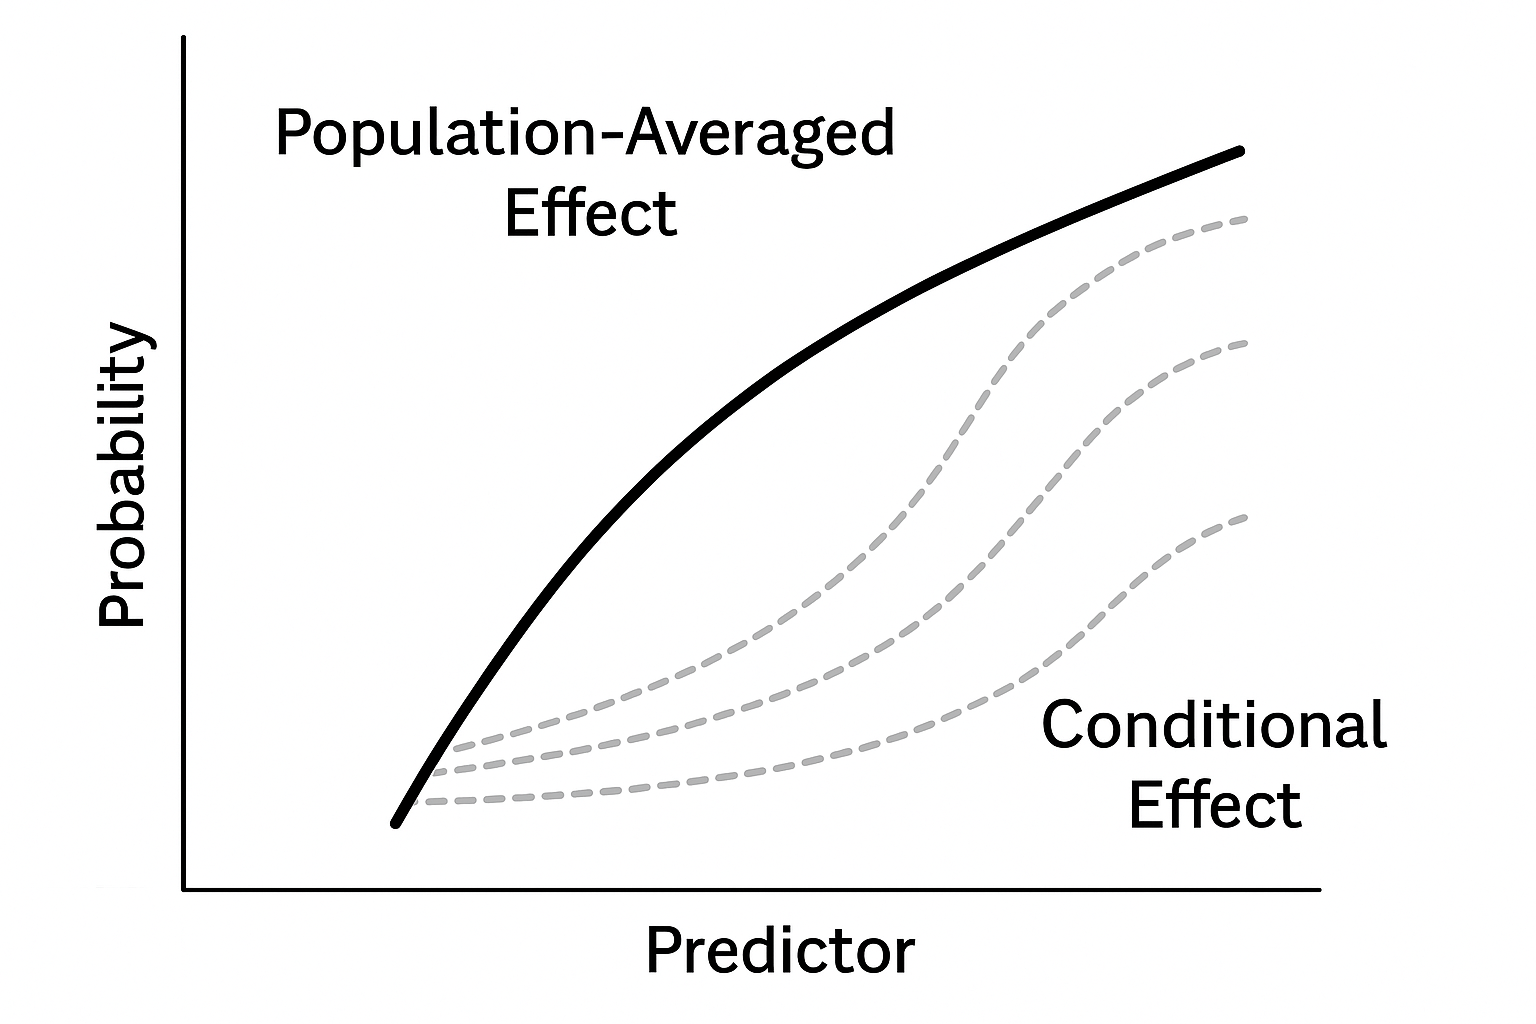
\includegraphics{fig/popfig.png}

}

\caption{Differences between population vs individual trajectories}

\end{figure}

In a \textbf{GLM}, we estimate the \textbf{marginal model}, where random
effects are integrated out or assumed zero:

\[ 
g(E[y_{ij}]) = \beta X_{ij},
\] which is interpreted as the
\textcolor{red}{population-averaged effect} or
\textcolor{blue}{marginal effect}. In contrast, a \textbf{GLMM}
estimates the slopes \textbf{conditional on random effects}:

\[
g(E[y_{ij}|\theta_i]) = \beta X_{ij} + \theta_i,                                       \]

where \(\theta_i\) accounts for subject-specific deviations. These are
known as \textcolor{blue}{conditional effects}. Because GLMs assume
independence, they can underestimate standard errors when clustering is
ignored.

To clarify the difference, consider the \textbf{subject-specific
(conditional)} expectation and the \textbf{population-averaged
(marginal)} expectation. For a given subject \(i\), the expected outcome
at observation \(j\) is

\[
E(y_{ij} \mid \theta_i) = g^{-1} \big( \beta_0 + \theta_i + \sum_{k=1}^p \beta x_{ijk} \big),                                                                                 \]

where \(g^{-1}\) is the inverse link function, \(\beta_0 + \theta_i\)
represents the subject-specific intercept, and the \(\beta x_{ijk}\)
terms are fixed effects. This expression defines an individual
trajectory, capturing how each subject deviates from the population
mean.

The \textbf{population-averaged mean} is obtained by integrating over
the distribution of random effects:

\[ 
E[y_{ij}] = E_{\theta_i} \left[ g^{-1} \big( \beta_0 + \theta_i + \beta'X_{ij} \big) \right].
\]

For non-linear link functions such as the logit, this is not equal to
simply applying \(g^{-1}\) to the fixed-effect part:

\[
E[g^{-1}(z)] \neq g^{-1}(E[z]).                                                         \]

This explains why the population-averaged curve (the black line in the
figure) does not match the mean of the subject-specific curves. The
non-linearity of \(g^{-1}\) causes averaging across individual
probabilities to produce a curve with a different shape. Thus, GLMs and
GLMMs provide fundamentally different interpretations of the
coefficients \(\beta\).

\begin{center}\rule{0.5\linewidth}{0.5pt}\end{center}

\hypertarget{poisson-regression-1}{%
\section*{Poisson Regression}\label{poisson-regression-1}}
\addcontentsline{toc}{section}{Poisson Regression}

\markright{Poisson Regression}

The \textbf{Poisson model} is used for \textbf{count data}, where each
observation \(y_i\) can take non-negative integer values
\(0, 1, 2, \dots\):

\[
y_i \sim \text{Poisson}(\theta_i) = \frac{e^{-\theta_i} \theta_i^{y_i}}{y_i!}.
\]

As with linear and logistic regression, the mean of \(y\) is related to
covariates through a \textbf{linear predictor}:

\[
\theta_i = \exp(X_i \beta).
\]

The \textbf{canonical link function} is the \textbf{log link}:

\[
g(\theta_i) = \log(\theta_i),
\]

which maps \((0, \infty) \rightarrow (-\infty, \infty)\) and ensures
predicted counts are positive.

\begin{tcolorbox}[enhanced jigsaw, rightrule=.15mm, breakable, left=2mm, colframe=quarto-callout-note-color-frame, opacityback=0, leftrule=.75mm, toprule=.15mm, colback=white, arc=.35mm, bottomrule=.15mm]

\textbf{Reminder: Differences from the Binomial Model}\vspace{2mm}

\begin{itemize}
\tightlist
\item
  \textbf{Binomial/logistic regression} is used when \(y_i\) represents
  the number of ``successes'' out of \(n_i\) trials (bounded count
  data).\\
\item
  \textbf{Poisson regression} is used when \(y_i\) is an unbounded count
  (e.g., number of events over time or space) and not based on a fixed
  number of trials. Commonly used to model rates
\end{itemize}

\end{tcolorbox}

\begin{center}\rule{0.5\linewidth}{0.5pt}\end{center}

\hypertarget{interpretation-of-poisson-regression}{%
\subsection*{Interpretation of Poisson
Regression}\label{interpretation-of-poisson-regression}}
\addcontentsline{toc}{subsection}{Interpretation of Poisson Regression}

Consider a simple model with one covariate:

\[
\begin{aligned}
y_i &\overset{\text{ind}}{\sim} \text{Poisson}(\lambda_i), \\
\log(\lambda_i) &= \beta_0 + \beta_1 x_i.
\end{aligned}
\]

\begin{itemize}
\tightlist
\item
  When \(x_i = 0\), the expected count is \(\lambda_i = e^{\beta_0}\).
\item
  For a one-unit change in \(x_i\): \[
  \beta_1 = \log(\lambda_i^*) - \log(\lambda_i),
  \] where \(\lambda_i^*\) is the expected count at \(x_i + 1\).
\item
  Therefore, \(e^{\beta_1}\) is the \textbf{incidence rate ratio (IRR)},
  the multiplicative change in expected counts for a unit increase in
  \(x_i\).
\item
  Covariate effects are \textbf{multiplicative}, not additive, on the
  original count scale.
\end{itemize}

\begin{center}\rule{0.5\linewidth}{0.5pt}\end{center}

\hypertarget{motivating-example-cancer-incidence-in-ohio}{%
\subsection*{Motivating Example: Cancer Incidence in
Ohio}\label{motivating-example-cancer-incidence-in-ohio}}
\addcontentsline{toc}{subsection}{Motivating Example: Cancer Incidence
in Ohio}

We analyze \textbf{lung cancer mortality} data across 88 counties in
Ohio, stratified by sex and race.

\textbf{Variables:}

\begin{itemize}
\tightlist
\item
  \(death_{stk}\): number of lung cancer deaths for population stratum
  \(k\) in county \(s\) during year \(t\),
\item
  \(sex_k\): 1 = female, 0 = male,
\item
  \(race_k\): 1 = white, 0 = non-white,
\item
  \(year_t\): 1--9 (1980--1988),
\item
  \(pop_{stk}\): population at risk.
\end{itemize}

\textbf{Research Questions:}

\begin{itemize}
\item
  How do sex and race affect lung cancer death counts?
\item
  How much variation exists between counties?
\item
  Can we estimate county-level risks (small-area estimation)?
\end{itemize}

We will fit a random-intercept Poisson regression model with a log link:

\[
\log E(death_{stk} \mid \theta_s) = \beta_0 + \beta_1 I_{\text{sex} = \text{female}} + \beta_2 I_{\text{race} = \text{white}} + \beta_3 \, \text{year}_t + \theta_s,
\]

where \(\theta_s \sim N(0, \tau^2)\) represents county-level random
intercepts, and \texttt{logpop} is included as an \textbf{offset} to
model lung cancer death rates rather than raw counts.

\begin{Shaded}
\begin{Highlighting}[]
\FunctionTok{library}\NormalTok{(lme4)}

\NormalTok{cancer }\OtherTok{\textless{}{-}} \FunctionTok{readRDS}\NormalTok{(}\FunctionTok{paste0}\NormalTok{(}\StringTok{"data/ohio\_cancer.RDS"}\NormalTok{))}
\FunctionTok{head}\NormalTok{(cancer)}
\end{Highlighting}
\end{Shaded}

\begin{verbatim}
  county sex race year death   pop
1      1   1    1    1     6  8912
2      1   1    1    2     5  9139
3      1   1    1    3     8  9455
4      1   1    1    4     5  9876
5      1   1    1    5     8 10281
6      1   1    1    6     5 10876
\end{verbatim}

\begin{Shaded}
\begin{Highlighting}[]
\CommentTok{\# Create offset for population at risk}
\NormalTok{cancer}\SpecialCharTok{$}\NormalTok{logpop }\OtherTok{\textless{}{-}} \FunctionTok{log}\NormalTok{(cancer}\SpecialCharTok{$}\NormalTok{pop)}

\CommentTok{\# Fit random{-}intercept Poisson model}
\NormalTok{fit\_poisson }\OtherTok{\textless{}{-}} \FunctionTok{glmer}\NormalTok{(}
\NormalTok{  death }\SpecialCharTok{\textasciitilde{}} \FunctionTok{offset}\NormalTok{(logpop) }\SpecialCharTok{+} \FunctionTok{factor}\NormalTok{(sex) }\SpecialCharTok{+} \FunctionTok{factor}\NormalTok{(race) }\SpecialCharTok{+}\NormalTok{ year }\SpecialCharTok{+}\NormalTok{ (}\DecValTok{1} \SpecialCharTok{|}\NormalTok{ county),}
  \AttributeTok{family =}\NormalTok{ poisson,}
  \AttributeTok{data =}\NormalTok{ cancer)}
\end{Highlighting}
\end{Shaded}

\begin{verbatim}
Warning in checkConv(attr(opt, "derivs"), opt$par, ctrl = control$checkConv, : Model is nearly unidentifiable: very large eigenvalue
 - Rescale variables?
\end{verbatim}

\begin{Shaded}
\begin{Highlighting}[]
\FunctionTok{summary}\NormalTok{(fit\_poisson)}
\end{Highlighting}
\end{Shaded}

\begin{verbatim}
Generalized linear mixed model fit by maximum likelihood (Laplace
  Approximation) [glmerMod]
 Family: poisson  ( log )
Formula: death ~ offset(logpop) + factor(sex) + factor(race) + year +  
    (1 | county)
   Data: cancer

     AIC      BIC   logLik deviance df.resid 
 26905.9  26940.4 -13447.9  26895.9     7387 

Scaled residuals: 
    Min      1Q  Median      3Q     Max 
-6.6678 -0.5699 -0.2176  0.3900 10.5059 

Random effects:
 Groups Name        Variance Std.Dev.
 county (Intercept) 0.0416   0.204   
Number of obs: 7392, groups:  county, 88

Fixed effects:
                Estimate Std. Error z value Pr(>|z|)    
(Intercept)   -7.7949302  0.0234154 -332.90  < 2e-16 ***
factor(sex)2  -1.1021170  0.0070715 -155.85  < 2e-16 ***
factor(race)2 -0.0474948  0.0103257   -4.60 4.23e-06 ***
year           0.0366854  0.0005224   70.22  < 2e-16 ***
---
Signif. codes:  0 '***' 0.001 '**' 0.01 '*' 0.05 '.' 0.1 ' ' 1

Correlation of Fixed Effects:
            (Intr) fctr(s)2 fctr(r)2
factor(sx)2 -0.077                  
factor(rc)2 -0.005 -0.005           
year        -0.278 -0.002   -0.036  
optimizer (Nelder_Mead) convergence code: 0 (OK)
Model is nearly unidentifiable: very large eigenvalue
 - Rescale variables?
\end{verbatim}

The warning \emph{``Model is nearly unidentifiable: very large
eigenvalue -- Rescale variables?''} indicates potential numerical
instability due to variables on very different scales or high
collinearity among predictors. Although the model converged, it is
recommended to \textbf{center or rescale continuous variables (e.g.,
\texttt{year})} to improve numerical conditioning and ensure stable
parameter estimation.

\begin{center}\rule{0.5\linewidth}{0.5pt}\end{center}

\textbf{Model Interpretations}

Fixed Effects:

\begin{itemize}
\item
  \textbf{Intercept (}\(\hat{\beta}_0 = -7.79\)):\\
  This is the \textbf{baseline log death rate} for non-white males in
  the reference year, in an average county.\\
  Converting to a rate:\\
  \[
  \exp(-7.79) \approx 0.00041,
  \] which is about 41 deaths per 100,000 people.
\item
  \textbf{Sex (female) (}\(\hat{\beta}_1 = -1.10\)):\\
  Holding race, year, and county constant, females have \textbf{67\%
  fewer deaths} compared to males:\\
  \[
  \exp(-1.10) \approx 0.33.
  \]
\item
  \textbf{Race (white) (}\(\hat{\beta}_2 = -0.047\)):\\
  White individuals have about \textbf{5\% fewer deaths} compared to
  non-white individuals:\\
  \[
  \exp(-0.047) \approx 0.95.
  \]
\item
  \textbf{Year (}\(\hat{\beta}_3 = 0.0367\)):\\
  Each year is associated with a \textbf{3.7\% increase} in lung cancer
  death rates, holding all other variables constant:\\
  \[
  \exp(0.0367) \approx 1.037.
  \]
\end{itemize}

Random Effects:

\begin{itemize}
\tightlist
\item
  \textbf{County-level variation (}\(\hat{\tau} = 0.204\)):\\
  The standard deviation of county-specific deviations in log death
  rates is 0.204.\\
  The middle 95\% of counties have baseline log rates within: \[
  -7.79 \pm 1.96 \cdot 0.204 = (-8.19, -7.39),
  \] which corresponds to rates ranging from approximately 0.00027 to
  0.00061 per person.
\end{itemize}

\begin{center}\rule{0.5\linewidth}{0.5pt}\end{center}

\hypertarget{overdispersion-of-the-poisson-assumption.-rcolorizeskip-red}{%
\subsection*{\texorpdfstring{Overdispersion of the Poisson Assumption.
\texttt{rcolorize("SKIP",\ "RED")}}{Overdispersion of the Poisson Assumption. rcolorize("SKIP", "RED")}}\label{overdispersion-of-the-poisson-assumption.-rcolorizeskip-red}}
\addcontentsline{toc}{subsection}{Overdispersion of the Poisson
Assumption. \texttt{rcolorize("SKIP",\ "RED")}}

\begin{itemize}
\item
  In Poisson, the assumption \(E(y_i) = V(y_i)\) is often violated!
\item
  One can add an additional \ul{overdispersion parameter} also called a
  \ul{scale parameter}.
\item
  One can adjust the parameter variance by this scale parameter. This is
  called the \textcolor{red}{quasi-poisson} model.

  \[
  \hat{\mathbf{\beta}} \sim N(\mathbf{\beta}, I(\mathbf{\beta})^{-1} \phi)
  \]
\item
  Fitting a quasi-poisson in GLM. Note: \texttt{glmer()} does not
  support a \texttt{quasipoisson} family --- quasi-likelihood does not
  extend cleanly to the numerical integration used to fit random effects
  --- so the scale-parameter adjustment is illustrated below with a
  standard (non-mixed) Poisson GLM rather than a GLMM.
\end{itemize}

\begin{Shaded}
\begin{Highlighting}[]
\NormalTok{glm\_quasi }\OtherTok{=} \FunctionTok{glm}\NormalTok{(death }\SpecialCharTok{\textasciitilde{}} \FunctionTok{offset}\NormalTok{(logpop) }\SpecialCharTok{+} \FunctionTok{factor}\NormalTok{(sex) }\SpecialCharTok{+} \FunctionTok{factor}\NormalTok{(race) }\SpecialCharTok{+}\NormalTok{ year,}
            \AttributeTok{family =}\NormalTok{ quasipoisson,}
            \AttributeTok{data =}\NormalTok{ cancer)}

\FunctionTok{summary}\NormalTok{(glm\_quasi)}
\end{Highlighting}
\end{Shaded}

\begin{verbatim}

Call:
glm(formula = death ~ offset(logpop) + factor(sex) + factor(race) + 
    year, family = quasipoisson, data = cancer)

Coefficients:
                Estimate Std. Error  t value Pr(>|t|)    
(Intercept)   -7.6886326  0.0092386 -832.233   <2e-16 ***
factor(sex)2  -1.0983692  0.0087951 -124.885   <2e-16 ***
factor(race)2  0.0440971  0.0124503    3.542    4e-04 ***
year           0.0357040  0.0006493   54.987   <2e-16 ***
---
Signif. codes:  0 '***' 0.001 '**' 0.01 '*' 0.05 '.' 0.1 ' ' 1

(Dispersion parameter for quasipoisson family taken to be 1.546573)

    Null deviance: 43628  on 7391  degrees of freedom
Residual deviance: 11323  on 7388  degrees of freedom
AIC: NA

Number of Fisher Scoring iterations: 4
\end{verbatim}

\begin{center}\rule{0.5\linewidth}{0.5pt}\end{center}

\hypertarget{section-9}{%
\section*{\texorpdfstring{\textcolor{purple}{Summary}}{}}\label{section-9}}
\addcontentsline{toc}{section}{\textcolor{purple}{Summary}}

\markright{\textcolor{purple}{Summary}}

\begin{longtable}[]{@{}
  >{\raggedright\arraybackslash}p{(\columnwidth - 2\tabcolsep) * \real{0.5000}}
  >{\raggedright\arraybackslash}p{(\columnwidth - 2\tabcolsep) * \real{0.5000}}@{}}
\toprule\noalign{}
\begin{minipage}[b]{\linewidth}\raggedright
\textbf{Section}
\end{minipage} & \begin{minipage}[b]{\linewidth}\raggedright
\textbf{Description}
\end{minipage} \\
\midrule\noalign{}
\endhead
\bottomrule\noalign{}
\endlastfoot
\textbf{What is the model?} & A \textbf{Generalized Linear Mixed Model
(GLMM)} extends GLMs by including \textbf{random effects} to account for
correlations within clusters (e.g., subjects, counties). The general
form is: \(g(E[y_{ij}|\theta_i]) = \beta_0 + x_{ij}'\beta + \theta_i\),
where \(\theta_i \sim N(0, \tau^2)\). \\
\textbf{Motivation} & Standard GLMs assume independent observations. In
real-world data, observations are often \textbf{correlated} (e.g.,
repeated measures, cluster data). Ignoring this leads to \textbf{biased
standard errors} and \textbf{invalid inference}. GLMMs address this by
modeling cluster-level variability. \\
\textbf{Model Components} & \textbf{1. Random component:} Distribution
from the exponential family (e.g., Binomial, Poisson). \textbf{2.
Systematic component:} Linear predictor
\(\eta_{ij} = \beta_0 + x_{ij}' \beta + \theta_i\). \textbf{3. Link
function:} \(g(\cdot)\) connects the mean response to the predictor. \\
\textbf{Likelihood} & The joint likelihood involves both fixed and
random effects:
\(L(\beta, \tau^2 | y) = \prod_i \int \left( \prod_j [y_{ij} | \theta_i] \right) [\theta_i] d\theta_i\).
Because this integral is difficult to solve, \textbf{numerical
approximation} (Laplace or adaptive quadrature) is used. \\
\textbf{Interpretation} & Fixed effects (\(\beta_j\)): Population-level
effects. Random effects (\(\theta_i\)): Group-specific deviations.
\textbf{GLM vs.~GLMM:} GLMs provide \textbf{population-averaged}
effects, while GLMMs provide \textbf{conditional} (subject-specific)
effects. \\
\textbf{Example: Crossover} & Logistic GLMM with a random intercept:
\(logit P(y_{ij}=1) = \beta_0 + \beta_1 \cdot \text{trt}_{ij} + \beta_2 \cdot \text{period}_{ij} + \beta_3 (\text{trt}\times \text{period})_{ij} + \theta_i\).
Highlights how ignoring correlation biases treatment effects. \\
\textbf{Model Comparisons} & \textbf{LRT:} Compares nested models via
\(\lambda_{LR} = -2 ( l_{reduced} - l_{full} ) \sim \chi^2_{df}\).
\textbf{AIC/BIC:} \(AIC = -2 l(\hat{\beta}) + 2p\), lower values
indicate better fit with complexity penalty. \\
\textbf{Poisson Regression} & For count data:
\(y_i \sim \text{Poisson}(\lambda_i)\), with
\(log(\lambda_i) = \beta_0 + x_i'\beta\). \textbf{Offsets:} Used to
model rates: \(log E(y_i) = log(N_i) + x_i' \beta\). \(e^{\beta_j}\) =
\textbf{Incidence Rate Ratio (IRR)}, a multiplicative change in expected
counts. \\
\textbf{Ohio Cancer Example} & Random-intercept Poisson GLMM:
\(log E(death_{stk} | \theta_s) = \beta_0 + \beta_1 \text{sex} + \beta_2 \text{race} + \beta_3 \text{year} + \theta_s + \log(pop_{stk})\).
Demonstrates county-level heterogeneity and interpretation of IRRs for
sex, race, and year. \\
\end{longtable}

\bookmarksetup{startatroot}

\hypertarget{module-2d-generalized-linear-mixed-models}{%
\chapter*{Module 2D Generalized Linear Mixed
Models}\label{module-2d-generalized-linear-mixed-models}}
\addcontentsline{toc}{chapter}{Module 2D Generalized Linear Mixed
Models}

\markboth{Module 2D Generalized Linear Mixed Models}{Module 2D
Generalized Linear Mixed Models}

\begin{verbatim}
Warning: package 'dplyr' was built under R version 4.4.3
\end{verbatim}

School data example adapted from Gelman and Hill.
\href{https://sites.stat.columbia.edu/gelman/arm/}{Data Analysis Using
Regression and Multilevel/Hierarchical Models}

Guatemalan data example: Rodriguez B and Goldman N (2001). Improved
estimation procedures for multilevel models with binary response: a case
study. Journal of Royal Statistical Society Series A 339-355.

\hypertarget{motivation-and-examples-4}{%
\subsection*{Motivation and Examples}\label{motivation-and-examples-4}}
\addcontentsline{toc}{subsection}{Motivation and Examples}

\begin{tcolorbox}[enhanced jigsaw, breakable, colbacktitle=quarto-callout-important-color!10!white, left=2mm, colframe=quarto-callout-important-color-frame, opacityback=0, coltitle=black, colback=white, rightrule=.15mm, title=\textcolor{quarto-callout-important-color}{\faExclamation}\hspace{0.5em}{Motivation:}, titlerule=0mm, opacitybacktitle=0.6, leftrule=.75mm, toprule=.15mm, arc=.35mm, bottomtitle=1mm, toptitle=1mm, bottomrule=.15mm]

\textbf{Hierarchical} or \textbf{multilevel} models are used when
observations are nested (.e.g, students within schools, repeated
measures within individuals). Standard regression models ignore
clustering, which leads to \textbf{underestimated standard errors} and
\textbf{biased inference}.

Hierarchical models can be thought of as GLMs that are reparametrized to
separate \textbf{with-in} group and \textbf{between} group sources of
variation with \textbf{nested} data structures. These include:

\begin{itemize}
\tightlist
\item
  Fixed effects for population-level estimates
\item
  Random effects for group-specific deviations.
\item
  Can have multiple levels within one model structure.
\end{itemize}

This has a very Bayesian Flavor! So it is more natural for me to think
this way.

\end{tcolorbox}

\hypertarget{motivating-example-school-math-scores}{%
\subsection*{Motivating Example: School Math
Scores}\label{motivating-example-school-math-scores}}
\addcontentsline{toc}{subsection}{Motivating Example: School Math
Scores}

We consider a three-level hierarchical model of math achievement data.

Levels:

\begin{itemize}
\item
  Level 1 (Year within child):

  \begin{itemize}
  \tightlist
  \item
    \(math_{ijk}\): standardized math score of child \(j\) in school
    \(i\) during year \(k\).
  \item
    \(year_{ijk}\): primary school year (centered at 3.5).
  \item
    \(retained_{ijk}\): indicator for repeating the grade.
  \end{itemize}
\item
  Level 2 (Child within school):

  \begin{itemize}
  \tightlist
  \item
    \(child_{ij}\): child ID.
  \item
    \(female_{ij}\): indicator for female.
  \item
    \(black_{ij}\), \(hispanic_{ij}\): race/ethnicity indicators.
  \end{itemize}
\item
  Level 3 (School):

  \begin{itemize}
  \tightlist
  \item
    \(school_i\): school ID.
  \item
    \(size_i\): number of students in school \(i\).
  \item
    \(lowinc_i\): percentage of low-income students in school \(i\).
  \end{itemize}
\end{itemize}

\begin{Shaded}
\begin{Highlighting}[]
\NormalTok{dat }\OtherTok{\textless{}{-}} \FunctionTok{read.csv}\NormalTok{(}\FunctionTok{paste0}\NormalTok{(}\FunctionTok{getwd}\NormalTok{(), }\StringTok{"/data/achievement.csv"}\NormalTok{))}
\FunctionTok{dim}\NormalTok{(dat)}
\end{Highlighting}
\end{Shaded}

\begin{verbatim}
[1] 7230   10
\end{verbatim}

\begin{Shaded}
\begin{Highlighting}[]
\NormalTok{dat[}\DecValTok{1}\SpecialCharTok{:}\DecValTok{6}\NormalTok{,]}
\end{Highlighting}
\end{Shaded}

\begin{verbatim}
  year   math retained female black hispanic size lowinc school child
1  0.5  1.146        0      0     0        1  380   40.3   2020   244
2  1.5  1.134        0      0     0        1  380   40.3   2020   244
3  2.5  2.300        0      0     0        1  380   40.3   2020   244
4 -1.5 -1.303        0      0     0        0  380   40.3   2020   248
5 -0.5  0.439        0      0     0        0  380   40.3   2020   248
6  0.5  2.430        0      0     0        0  380   40.3   2020   248
\end{verbatim}

\begin{Shaded}
\begin{Highlighting}[]
\FunctionTok{ggplot}\NormalTok{(dat, }\FunctionTok{aes}\NormalTok{(}\AttributeTok{x =}\NormalTok{ year, }\AttributeTok{y =}\NormalTok{ math, }\AttributeTok{group =}\NormalTok{ child, }\AttributeTok{color =} \FunctionTok{factor}\NormalTok{(school))) }\SpecialCharTok{+}
  \FunctionTok{geom\_line}\NormalTok{(}\AttributeTok{alpha =} \FloatTok{0.4}\NormalTok{) }\SpecialCharTok{+}      \CommentTok{\# line for each student\textquotesingle{}s trajectory}
  \FunctionTok{geom\_point}\NormalTok{(}\AttributeTok{alpha =} \FloatTok{0.6}\NormalTok{) }\SpecialCharTok{+}     \CommentTok{\# points for observations}
  \FunctionTok{labs}\NormalTok{(}
    \AttributeTok{title =} \StringTok{"Student Math Scores Over Time"}\NormalTok{,}
    \AttributeTok{x =} \StringTok{"Year"}\NormalTok{,}
    \AttributeTok{y =} \StringTok{"Math Score"}\NormalTok{,}
    \AttributeTok{color =} \StringTok{"School"}
\NormalTok{  ) }\SpecialCharTok{+}
  \FunctionTok{theme\_minimal}\NormalTok{() }\SpecialCharTok{+}
  \FunctionTok{theme}\NormalTok{(}\AttributeTok{legend.position =} \StringTok{"none"}\NormalTok{)}
\end{Highlighting}
\end{Shaded}

\begin{figure}[H]

{\centering 
\includegraphics{Module_2D_GLMMs_files/figure-pdf/unnamed-chunk-2-1.pdf}

}

\end{figure}

The plot above shows individual trajectories of student scores across
years. Colors denote school.

\begin{center}\rule{0.5\linewidth}{0.5pt}\end{center}

\hypertarget{fitting-a-linear-mixed-model}{%
\subsection*{Fitting a Linear Mixed
Model}\label{fitting-a-linear-mixed-model}}
\addcontentsline{toc}{subsection}{Fitting a Linear Mixed Model}

Using the methods we have learned so far, we would fit a linear mixed
model (LMM). We can include a random intercept model to account for
student-specific differences in baseline math scores:

\[
\text{math}_{ijk} = \beta_0 + \beta_1 \, \text{year}_{ijk} + \beta_2 \, \text{female}_{ij} + \beta_3 \, \text{black}_{ij} + \beta_4 \, \text{hispanic}_{ij} + \beta_5 \, \text{retained}_{ij} + u_{i} + \epsilon_{ijk},
\]

where:\\
- \(i\) indexes students within school \(j\),\\
- \(u_{i} \sim N(0, \tau^2)\) is a \textbf{student-specific random
intercept},\\
- \(\epsilon_{ijk} \sim N(0, \sigma^2)\) is the residual error term.

This model \emph{partially pools} the intercepts across students,
borrowing strength from the entire dataset while still allowing each
student to have its own baseline.

\textcolor{red}{Problem!}: Years are \textbf{nested within students},
and \textbf{students are nested within schools}. In other words, the
math scores are measured repeatedly for each student (longitudinal
data), and these students are clustered within schools. So even if we
account for within student correlation, we have not accounted for within
school correlation. A standard LLM fails to account for this
hierarchical data structure.

\begin{center}\rule{0.5\linewidth}{0.5pt}\end{center}

\hypertarget{the-better-approach-three-level-linear-mixed-model}{%
\subsection*{The Better Approach: Three Level Linear Mixed
Model}\label{the-better-approach-three-level-linear-mixed-model}}
\addcontentsline{toc}{subsection}{The Better Approach: Three Level
Linear Mixed Model}

We extend the previous model to account for \textbf{both student-level
and school-level random intercepts}, fully respecting the data hierarchy
(years within students, and students within schools).

\[
\begin{align*}
math_{ijk} & \sim Normal(\mu_{ijk}, \sigma^2)\\
\mu_{ijk} & = \beta_0 + \beta_1 \, \text{year}_{ijk} + \beta_2 \, \text{female}_{ij} + \beta_3 \, \text{black}_{ij} + \beta_4 \, \text{hispanic}_{ij} + \beta_5 \, \text{retained}_{ij} + \underbrace{u_{i}}_{\text{school}}  + \underbrace{u_{ij}}_{\text{student within school}},\\
u_{ij} & \overset{iid}{\sim} N(0, \tau^2)\\
u_i & \overset{iid}{\sim} N(0, \nu^2)\\
\epsilon_{ijk} & \overset{iid}{\sim} N(0, \sigma^2). \quad \text{residual error for year-student-school}
\end{align*}
\]

We can think of \(u_i\) and \(u_{ij}\) as parameters that control for
\textcolor{red}{unmeasured confounders} at the school and student level.

\emph{``One statistician's mean structure is another's covariance
structure.'' (Donald Rubin)}

\begin{itemize}
\item
  In \textbf{frequentist mixed models}, random effects are viewed as
  part of the \textbf{covariance structure} because they induce
  correlation between observations within a cluster. The random effects
  are integrated out when estimating the model, and their variability
  (e.g., \(\tau^2\)) contributes to the marginal covariance matrix.
\item
  In \textbf{Bayesian or hierarchical modeling}, the same random effects
  are treated as part of the \textbf{mean structure} with unknown
  parameters that have prior distributions. We estimate the full
  posterior for both fixed effects and random effects.
\item
  For example, in a linear mixed model:
\end{itemize}

\[
y_{ij} = \beta_0 + \beta_1 x_{ij} + u_i + \epsilon_{ij},
\]

we can think of:

\begin{itemize}
\item
  \textbf{Bayesian method:} \(u_i\) is a \textbf{random deviation} that
  adjusts the mean for cluster \(i\) (part of the mean structure). In
  our 3-level LMM, we place priors on both population-level parameters
  and random effects, e.g., \(\beta_k \sim N(0, 10^2)\).
\item
  \textbf{Frequentist method:} Equivalently, \ul{the marginal
  distribution of \(y_{ij}\)} can be expressed as:
\end{itemize}

\[
y_{ij} \sim N\!\big(\beta_0 + \beta_1 x_{ij}, \ \tau^2 + \sigma^2\big),
\]

where the extra variance \(\tau^2\) is part of the \textbf{covariance
structure}. We refer to the marginal distribution because in the
frequentist approach the random effects are integrated out, and the
variability they induce enters the covariance structure.

\begin{itemize}
\tightlist
\item
  In our 3-level LMM, these random effects are treated as components
  that induce correlation but are not explicitly estimated as
  parameters.
\end{itemize}

\begin{center}\rule{0.5\linewidth}{0.5pt}\end{center}

\hypertarget{pooling-borrowing-information-at-multiple-levels}{%
\subsection*{Pooling (Borrowing Information) at Multiple
Levels}\label{pooling-borrowing-information-at-multiple-levels}}
\addcontentsline{toc}{subsection}{Pooling (Borrowing Information) at
Multiple Levels}

Our three-level linear mixed model: \[
math_{ijk} = \beta_0 + \beta_1 year_{ijk} + \cdots + u_i + u_{ij} + \epsilon_{ijk},
\] borrows strength across both \textbf{schools} (Level 3) and
\textbf{students} (Level 2). This is known as \textbf{multi-level
partial pooling}.

\hypertarget{pooling-across-schools}{%
\subsubsection*{1. Pooling Across
Schools}\label{pooling-across-schools}}
\addcontentsline{toc}{subsubsection}{1. Pooling Across Schools}

\begin{itemize}
\item
  \textbf{No pooling (separate means):} Each school mean is just its
  sample mean: \[
  \hat{\mu}_i^{\text{no-pool}} = \bar{y}_i.
  \]
\item
  \textbf{Complete pooling (one mean):} All schools share the overall
  mean: \[
  \hat{\mu}_i^{\text{complete-pool}} = \bar{y}.
  \]
\item
  \textbf{Partial pooling (hierarchical):} \[
  \hat{\mu}_i^{\text{partial-pool}} = w_i \, \bar{y}_i + (1 - w_i)\, \bar{y},
  \] where \[
  w_i = \frac{n_i}{n_i + \frac{\sigma^2}{\nu^2}},
  \] with \(n_i\) = number of observations in school \(i\), \(\nu^2\) =
  between-school variance, and \(\sigma^2\) = residual variance.

  \begin{itemize}
  \tightlist
  \item
    Large schools (big \(n_i\)) get \(w_i \approx 1\) (close to
    \textbf{no pooling}).
  \item
    Small schools (small \(n_i\)) get \(w_i \approx 0\) (closer to
    \textbf{complete pooling}).
  \end{itemize}
\end{itemize}

\hypertarget{pooling-across-students-within-schools}{%
\subsubsection*{2. Pooling Across Students (Within
Schools)}\label{pooling-across-students-within-schools}}
\addcontentsline{toc}{subsubsection}{2. Pooling Across Students (Within
Schools)}

Within each school \(i\), we also pool across students \(j\): \[
  \hat{u}_{ij}^{\text{partial}} = w_{ij} \, (\bar{y}_{ij} - \bar{y}_i),
  \] where \[
  w_{ij} = \frac{n_{ij}}{n_{ij} + \frac{\sigma^2}{\tau^2}},
  \] with \(n_{ij}\) = number of observations for student \(j\), and
\(\tau^2\) = student-level variance.

\begin{tcolorbox}[enhanced jigsaw, rightrule=.15mm, breakable, left=2mm, colframe=quarto-callout-tip-color-frame, opacityback=0, leftrule=.75mm, toprule=.15mm, colback=white, arc=.35mm, bottomrule=.15mm]

\textbf{Derivation of student-level partially pooled
estimate}\vspace{2mm}

\hypertarget{step-1-define-the-student-mean}{%
\subsubsection*{Step 1: Define the Student
Mean}\label{step-1-define-the-student-mean}}
\addcontentsline{toc}{subsubsection}{Step 1: Define the Student Mean}

For student \(j\) in school \(i\), the average math score is: \[
\bar{y}_{ij} = \frac{1}{n_{ij}} \sum_{k=1}^{n_{ij}} math_{ijk}.
\]

Substituting the model: \[
\bar{y}_{ij} = \beta_0 + u_i + u_{ij} + \frac{1}{n_{ij}} \sum_{k=1}^{n_{ij}} \epsilon_{ijk}.
\]

Define the \textbf{average residual error}: \[
\bar{\epsilon}_{ij} = \frac{1}{n_{ij}} \sum_{k=1}^{n_{ij}} \epsilon_{ijk},
\] which satisfies \(\bar{\epsilon}_{ij} \sim N(0, \sigma^2 / n_{ij})\).

\begin{center}\rule{0.5\linewidth}{0.5pt}\end{center}

\hypertarget{step-2-center-by-the-school-mean}{%
\subsubsection*{Step 2: Center by the School
Mean}\label{step-2-center-by-the-school-mean}}
\addcontentsline{toc}{subsubsection}{Step 2: Center by the School Mean}

Subtract the school mean \(\bar{y}_i\) (which contains
\(\beta_0 + u_i\)): \[
\bar{y}_{ij} - \bar{y}_i = u_{ij} + \bar{\epsilon}_{ij}.
\]

This shows that a student's deviation from the school mean is driven by:
- The student's random effect \(u_{ij}\), - The average residual noise
\(\bar{\epsilon}_{ij}\).

\begin{center}\rule{0.5\linewidth}{0.5pt}\end{center}

\hypertarget{step-3-target-quantity}{%
\subsubsection*{Step 3: Target Quantity}\label{step-3-target-quantity}}
\addcontentsline{toc}{subsubsection}{Step 3: Target Quantity}

We want the posterior mean of \(u_{ij}\) given the observed deviation:
\[
\hat{u}_{ij}^{\text{partial}} = E[ u_{ij} \mid \bar{y}_{ij} - \bar{y}_i ].
\]

The prior and likelihood are: \[
u_{ij} \sim N(0, \tau^2),
\] \[
\bar{y}_{ij} - \bar{y}_i \mid u_{ij} \sim N(u_{ij}, \sigma^2 / n_{ij}).
\]

\begin{center}\rule{0.5\linewidth}{0.5pt}\end{center}

\hypertarget{step-4-conditional-expectation}{%
\subsubsection*{Step 4: Conditional
Expectation}\label{step-4-conditional-expectation}}
\addcontentsline{toc}{subsubsection}{Step 4: Conditional Expectation}

For a bivariate normal vector \((U, Y)\): \[
E[U \mid Y] = \frac{\text{Cov}(U, Y)}{\text{Var}(Y)} \,(Y - E[Y]) + E[U].
\]

Here, \(U = u_{ij}\), \(Y = \bar{y}_{ij} - \bar{y}_i\), and
\(E[U] = 0\): \[
\text{Var}(Y) = \text{Var}(u_{ij} + \bar{\epsilon}_{ij}) = \tau^2 + \frac{\sigma^2}{n_{ij}},
\] \[
\text{Cov}(u_{ij}, Y) = \text{Cov}(u_{ij}, u_{ij} + \bar{\epsilon}_{ij}) = \tau^2.
\]

Thus: \[
E[u_{ij} \mid \bar{y}_{ij} - \bar{y}_i] =
\frac{\tau^2}{\tau^2 + \sigma^2 / n_{ij}} (\bar{y}_{ij} - \bar{y}_i).
\]

\begin{center}\rule{0.5\linewidth}{0.5pt}\end{center}

\hypertarget{step-5-shrinkage-weight}{%
\subsubsection*{Step 5: Shrinkage
Weight}\label{step-5-shrinkage-weight}}
\addcontentsline{toc}{subsubsection}{Step 5: Shrinkage Weight}

Define: \[
w_{ij} = \frac{\tau^2}{\tau^2 + \sigma^2 / n_{ij}} = \frac{n_{ij}}{n_{ij} + \frac{\sigma^2}{\tau^2}},
\] so the \textbf{partially pooled student intercept} is: \[
\hat{u}_{ij}^{\text{partial}} = w_{ij} (\bar{y}_{ij} - \bar{y}_i).
\]

\end{tcolorbox}

\begin{itemize}
\item
  \textbf{Students with more data} (\(n_{ij}\) large) →
  \(w_{ij} \approx 1\), so their random intercept is close to their own
  average.
\item
  \textbf{Students with sparse data} (\(n_{ij}\) small) →
  \(w_{ij} \approx 0\), so their intercept is shrunk toward the
  \textbf{school-level mean}.
\item
  The \textbf{random intercepts} \(u_i\) and \(u_{ij}\) ensure that the
  model combines information from all schools and students.\\
\item
  Small or noisy groups borrow strength from the larger dataset, which
  improves stability and reduces overfitting.
\end{itemize}

We can visualize this with a \textbf{shrinkage plot} showing raw school
means vs.~partially pooled estimates, as well as student-level
intercepts:


\includegraphics{Module_2D_GLMMs_files/figure-pdf/unnamed-chunk-3-1.pdf}

\begin{center}\rule{0.5\linewidth}{0.5pt}\end{center}

\hypertarget{covariance-structures-in-hierarchical-glmms}{%
\subsection*{Covariance Structures in Hierarchical
GLMMs}\label{covariance-structures-in-hierarchical-glmms}}
\addcontentsline{toc}{subsection}{Covariance Structures in Hierarchical
GLMMs}

For the \textbf{three-level linear mixed model}:

\[
\begin{aligned}
math_{ijk} &\sim \text{Normal}(\mu_{ijk}, \sigma^2), \\
\mu_{ijk} &= \beta_0 + u_i + u_{ij} + \beta_1' x_{ijk} + \beta_2' x_{ij} + \beta_3' x_i, \\
u_i &\sim N(0, \nu^2), \quad u_{ij} \sim N(0, \tau^2),
\end{aligned}
\]

where:

\begin{itemize}
\tightlist
\item
  \(u_i\) is the \textbf{school-level random intercept},
\item
  \(u_{ij}\) is the \textbf{student-level random intercept} (nested
  within school \(i\)),
\item
  \(\sigma^2\) is the residual (Level 1) variance for observations
  within a student.
\end{itemize}

\begin{center}\rule{0.5\linewidth}{0.5pt}\end{center}

\hypertarget{conditional-variance}{%
\paragraph*{Conditional Variance}\label{conditional-variance}}
\addcontentsline{toc}{paragraph}{Conditional Variance}

Conditioned on the random effects \(u_i\) and \(u_{ij}\), the
distribution of \(math_{ijk}\) is:

\[
math_{ijk}|u_i, u_{ij} \sim N(\mu_{ijk}, \sigma^2)
\]

where \(\mu_{ijk}\) is the linear predictor: \[
E(math_{ijk}|u_i, u_{ij}) = \mu_{ijk} = \beta_0 + \beta^{(1)'} x_{ijk} + \beta^{(2)'} x_{ij} + u_i + u_{ij},
\] and \[
Var(math_{ijk} \mid u_i, u_{ij}) = \sigma^2,
\]

\begin{tcolorbox}[enhanced jigsaw, rightrule=.15mm, breakable, left=2mm, colframe=quarto-callout-tip-color-frame, opacityback=0, leftrule=.75mm, toprule=.15mm, colback=white, arc=.35mm, bottomrule=.15mm]

\textbf{Derivation of conditional variance}\vspace{2mm}

Conditioned on the random effects \(u_i\) and \(u_{ij}\), we can write:
\[
math_{ijk} \mid u_i, u_{ij} = \mu_{ijk} + \epsilon_{ijk}.
\]

Since \(\mu_{ijk}\) is treated as fixed once we condition on \(u_i\) and
\(u_{ij}\), the only remaining random component is \(\epsilon_{ijk}\).
Therefore: \[
\begin{aligned}
Var(math_{ijk} \mid u_i, u_{ij}) 
&= Var(\mu_{ijk} + \epsilon_{ijk} \mid u_i, u_{ij}) \\
&= Var(\epsilon_{ijk}) \\
&= \sigma^2.
\end{aligned}
\]

\end{tcolorbox}

\begin{center}\rule{0.5\linewidth}{0.5pt}\end{center}

\hypertarget{total-variance}{%
\paragraph*{Total Variance}\label{total-variance}}
\addcontentsline{toc}{paragraph}{Total Variance}

This variance \(\sigma^2\) describes the \textbf{Level 1 variability
(within-student, across years)}, assuming the random effects \(u_i\) and
\(u_{ij}\) are fixed.

The \textbf{total variability} in \(math_{ijk}\) can be decomposed into:

\[
Var(math_{ijk}) = \nu^2 + \tau^2 + \sigma^2,
\]

where:

\begin{itemize}
\tightlist
\item
  \(\nu^2\) reflects \textbf{between-school variability},
\item
  \(\tau^2\) reflects \textbf{between-student variability (within
  school)},
\item
  \(\sigma^2\) reflects \textbf{within-student residual variability}.
\end{itemize}

\begin{tcolorbox}[enhanced jigsaw, rightrule=.15mm, breakable, left=2mm, colframe=quarto-callout-tip-color-frame, opacityback=0, leftrule=.75mm, toprule=.15mm, colback=white, arc=.35mm, bottomrule=.15mm]

\textbf{Derivation of Total Variance}\vspace{2mm}

For the three-level linear mixed model: \[
math_{ijk} = \beta_0 + \beta_1 \, year_{ijk} + \cdots + u_i + u_{ij} + \epsilon_{ijk},
\] we assume: \[
u_i \sim N(0, \nu^2), \quad u_{ij} \sim N(0, \tau^2), \quad \epsilon_{ijk} \sim N(0, \sigma^2),
\] with all random components \textbf{mutually independent}.

We want to show that: \[
Var(math_{ijk}) = \nu^2 + \tau^2 + \sigma^2.
\]

\begin{center}\rule{0.5\linewidth}{0.5pt}\end{center}

\hypertarget{step-1-apply-the-law-of-total-variance}{%
\subsubsection*{Step 1: Apply the Law of Total
Variance}\label{step-1-apply-the-law-of-total-variance}}
\addcontentsline{toc}{subsubsection}{Step 1: Apply the Law of Total
Variance}

The law of total variance states: \[
Var(Y) = E[Var(Y \mid U)] + Var(E[Y \mid U]),
\] where \(U\) represents any random variables we are conditioning on.

In our case, we condition on both \(u_i\) and \(u_{ij}\): \[
Var(math_{ijk}) = E[Var(math_{ijk} \mid u_i, u_{ij})] + Var(E[math_{ijk} \mid u_i, u_{ij}]).
\]

\begin{center}\rule{0.5\linewidth}{0.5pt}\end{center}

\hypertarget{step-2-compute-the-conditional-variance}{%
\subsubsection*{Step 2: Compute the Conditional
Variance}\label{step-2-compute-the-conditional-variance}}
\addcontentsline{toc}{subsubsection}{Step 2: Compute the Conditional
Variance}

From the model: \[
math_{ijk} \mid u_i, u_{ij} = \mu_{ijk} + \epsilon_{ijk},
\] where
\(\mu_{ijk} = \beta_0 + \beta_1 \, year_{ijk} + \cdots + u_i + u_{ij}\).

Conditioned on \(u_i\) and \(u_{ij}\), the only random term is
\(\epsilon_{ijk}\), so: \[
Var(math_{ijk} \mid u_i, u_{ij}) = Var(\epsilon_{ijk}) = \sigma^2.
\] Therefore: \[
E[Var(math_{ijk} \mid u_i, u_{ij})] = \sigma^2.
\]

\begin{center}\rule{0.5\linewidth}{0.5pt}\end{center}

\hypertarget{step-3-compute-the-variance-of-the-conditional-expectation}{%
\subsubsection*{Step 3: Compute the Variance of the Conditional
Expectation}\label{step-3-compute-the-variance-of-the-conditional-expectation}}
\addcontentsline{toc}{subsubsection}{Step 3: Compute the Variance of the
Conditional Expectation}

The conditional expectation is: \[
E[math_{ijk} \mid u_i, u_{ij}] = \mu_{ijk} = \beta_0 + \beta_1 \, year_{ijk} + \cdots + u_i + u_{ij}.
\]

The fixed terms \(\beta_0 + \beta_1 \, year_{ijk} + \cdots\) have no
variance, so: \[
Var(E[math_{ijk} \mid u_i, u_{ij}]) = Var(u_i + u_{ij}) = Var(u_i) + Var(u_{ij}),
\] because \(u_i\) and \(u_{ij}\) are independent. Thus: \[
Var(E[math_{ijk} \mid u_i, u_{ij}]) = \nu^2 + \tau^2.
\]

\begin{center}\rule{0.5\linewidth}{0.5pt}\end{center}

\hypertarget{step-4-combine-results}{%
\subsubsection*{Step 4: Combine Results}\label{step-4-combine-results}}
\addcontentsline{toc}{subsubsection}{Step 4: Combine Results}

Putting it all together: \[
Var(math_{ijk}) = E[Var(math_{ijk} \mid u_i, u_{ij})] + Var(E[math_{ijk} \mid u_i, u_{ij}])
= \sigma^2 + (\nu^2 + \tau^2)
= \nu^2 + \tau^2 + \sigma^2.
\]

\end{tcolorbox}

\begin{center}\rule{0.5\linewidth}{0.5pt}\end{center}

\hypertarget{conditional-vs.-marginal-covariance}{%
\subsubsection*{Conditional vs.~Marginal
Covariance}\label{conditional-vs.-marginal-covariance}}
\addcontentsline{toc}{subsubsection}{Conditional vs.~Marginal
Covariance}

For two observations \(math_{ijk}\) and \(math_{ijk'}\) from the
\textbf{same student} \(j\) in the \textbf{same school} \(i\): \[
Cov(math_{ijk}, math_{ijk'} \mid u_i, u_{ij}) = 0,
\] because, conditioned on \(u_i\) and \(u_{ij}\), the residual errors
\(\epsilon_{ijk}\) are independent.

However, the \textbf{marginal covariance} (after integrating over the
random effects) is: \[
Cov(math_{ijk}, math_{ijk'}) = \nu^2 + \tau^2,
\] since both observations share \(u_i\) (school effect) and \(u_{ij}\)
(student effect).

For two students \(j \neq j'\) in the \textbf{same school} \(i\): \[
Cov(math_{ijk}, math_{ij'k'}) = \nu^2,
\] because they share only the school effect \(u_i\).

\begin{center}\rule{0.5\linewidth}{0.5pt}\end{center}

\hypertarget{intraclass-correlation-coefficients-icc}{%
\subsection*{Intraclass Correlation Coefficients
(ICC)}\label{intraclass-correlation-coefficients-icc}}
\addcontentsline{toc}{subsection}{Intraclass Correlation Coefficients
(ICC)}

The total variance of \(math_{ijk}\) is: \[
Var(math_{ijk}) = \nu^2 + \tau^2 + \sigma^2.
\]

The \textbf{school-level intraclass correlation (ICC)}, which measures
the proportion of variance explained by differences between schools, is:
\[
ICC_{\text{school}} = \frac{\nu^2}{\nu^2 + \tau^2 + \sigma^2}.
\]

The \textbf{student-level ICC (within a school)} is: \[
ICC_{\text{student}} = \frac{\nu^2 + \tau^2}{\nu^2 + \tau^2 + \sigma^2}.
\]

These ICCs quantify how strongly scores are correlated for students
within the same school or the same student across multiple years.

\begin{center}\rule{0.5\linewidth}{0.5pt}\end{center}

\hypertarget{hierarchical-glmm-fitting-in-r}{%
\subsection*{Hierarchical GLMM Fitting in
R}\label{hierarchical-glmm-fitting-in-r}}
\addcontentsline{toc}{subsection}{Hierarchical GLMM Fitting in R}

\begin{Shaded}
\begin{Highlighting}[]
\CommentTok{\# Load required package}
\FunctionTok{library}\NormalTok{(lme4)}

\CommentTok{\# Fit the 3{-}level LMM}
\CommentTok{\# math \textasciitilde{} fixed effects + (1 | school/child) fits random intercepts for school and child}
\NormalTok{lmm\_3level }\OtherTok{\textless{}{-}} \FunctionTok{lmer}\NormalTok{(}
\NormalTok{  math }\SpecialCharTok{\textasciitilde{}}\NormalTok{ year }\SpecialCharTok{+}\NormalTok{ female }\SpecialCharTok{+}\NormalTok{ black }\SpecialCharTok{+}\NormalTok{ hispanic }\SpecialCharTok{+}\NormalTok{ retained }\SpecialCharTok{+} 
\NormalTok{    (}\DecValTok{1} \SpecialCharTok{|}\NormalTok{ school}\SpecialCharTok{/}\NormalTok{child),  }\CommentTok{\# child is nested within school}
  \AttributeTok{data =}\NormalTok{ dat}
\NormalTok{)}

\CommentTok{\# Display model summary}
\FunctionTok{summary}\NormalTok{(lmm\_3level)}
\end{Highlighting}
\end{Shaded}

\begin{verbatim}
Linear mixed model fit by REML ['lmerMod']
Formula: 
math ~ year + female + black + hispanic + retained + (1 | school/child)
   Data: dat

REML criterion at convergence: 16699.2

Scaled residuals: 
    Min      1Q  Median      3Q     Max 
-3.8443 -0.5854 -0.0272  0.5588  6.1663 

Random effects:
 Groups       Name        Variance Std.Dev.
 child:school (Intercept) 0.6638   0.8148  
 school       (Intercept) 0.1292   0.3594  
 Residual                 0.3445   0.5870  
Number of obs: 7230, groups:  child:school, 1721; school, 60

Fixed effects:
              Estimate Std. Error t value
(Intercept) -3.477e-01  8.095e-02  -4.295
year         7.483e-01  5.396e-03 138.677
female       8.850e-06  4.226e-02   0.000
black       -6.235e-01  7.873e-02  -7.919
hispanic    -3.636e-01  8.813e-02  -4.125
retained     1.487e-01  3.536e-02   4.207

Correlation of Fixed Effects:
         (Intr) year   female black  hispnc
year     -0.020                            
female   -0.264 -0.005                     
black    -0.691 -0.004 -0.003              
hispanic -0.515 -0.009  0.019  0.519       
retained -0.020  0.086  0.017 -0.015 -0.007
\end{verbatim}

\hypertarget{model-interpretations}{%
\subsection*{Model Interpretations}\label{model-interpretations}}
\addcontentsline{toc}{subsection}{Model Interpretations}

\hypertarget{random-effects}{%
\subsubsection*{Random Effects}\label{random-effects}}
\addcontentsline{toc}{subsubsection}{Random Effects}

\begin{itemize}
\item
  \textbf{School-level variance (}\(\nu^2 = 0.1292\)):\\
  Differences between schools account for some variation in math scores
  (Std. Dev. = 0.359).\\
  This suggests that students from different schools start at different
  baseline math levels.
\item
  \textbf{Student-level variance (}\(\tau^2 = 0.6638\)):\\
  Differences between students (within schools) account for a larger
  portion of variability (Std. Dev. = 0.815), indicating substantial
  heterogeneity across students.
\item
  \textbf{Residual variance (}\(\sigma^2 = 0.3445\)):\\
  Variation in math scores within the same student (across years) after
  accounting for predictors is 0.3445 (Std. Dev. = 0.587).
\item
  \textbf{Number of groups:}\\
  There are 60 schools and 1,721 students across 7,230 total
  observations.
\end{itemize}

\hypertarget{fixed-effects}{%
\subsubsection*{Fixed Effects}\label{fixed-effects}}
\addcontentsline{toc}{subsubsection}{Fixed Effects}

\begin{itemize}
\item
  \textbf{Intercept (-0.348):}\\
  The expected math score for a reference student (male, non-Black,
  non-Hispanic, not retained) in year 0 is -0.35 (on the standardized
  scale).
\item
  \textbf{Year (0.748):}\\
  On average, math scores increase by 0.748 units per year,
  \textbf{holding all other factors constant}.\\
  This is a \textbf{strong positive trend} over time (t = 138.7).
\item
  \textbf{Female (0.00001):}\\
  The coefficient for being female is nearly zero (and not statistically
  significant).
\item
  \textbf{Black (-0.623):}\\
  Black students have an average math score 0.62 units lower than
  non-Black students, holding other variables constant (t = -7.92).
\item
  \textbf{Hispanic (-0.364):}\\
  Hispanic students have an average math score 0.36 units lower than
  non-Hispanic students (t = -4.13).
\item
  \textbf{Retained (0.149):}\\
  Students who were retained (repeated a grade) have math scores
  approximately 0.15 units higher than otherwise similar students (t =
  4.21). This may reflect additional time or intervention effects.
\end{itemize}

We can calculate ICCs directly from the variance components of the
model:

\begin{Shaded}
\begin{Highlighting}[]
\CommentTok{\# Extract variance components}
\NormalTok{vc }\OtherTok{\textless{}{-}} \FunctionTok{as.data.frame}\NormalTok{(}\FunctionTok{VarCorr}\NormalTok{(lmm\_3level))}

\CommentTok{\# Variance components}
\NormalTok{var\_school  }\OtherTok{\textless{}{-}}\NormalTok{ vc[vc}\SpecialCharTok{$}\NormalTok{grp }\SpecialCharTok{==} \StringTok{"school"}\NormalTok{, }\StringTok{"vcov"}\NormalTok{]         }\CommentTok{\# ν² (between schools)}
\NormalTok{var\_child   }\OtherTok{\textless{}{-}}\NormalTok{ vc[vc}\SpecialCharTok{$}\NormalTok{grp }\SpecialCharTok{==} \StringTok{"child:school"}\NormalTok{, }\StringTok{"vcov"}\NormalTok{]   }\CommentTok{\# τ² (between students within schools)}
\NormalTok{var\_resid  }\OtherTok{\textless{}{-}}\NormalTok{ vc[vc}\SpecialCharTok{$}\NormalTok{grp }\SpecialCharTok{==} \StringTok{"Residual"}\NormalTok{, }\StringTok{"vcov"}\NormalTok{]      }\CommentTok{\# σ² (within students)}

\CommentTok{\# Total variance}
\NormalTok{var\_total }\OtherTok{\textless{}{-}}\NormalTok{ var\_school }\SpecialCharTok{+}\NormalTok{ var\_child }\SpecialCharTok{+}\NormalTok{ var\_resid}

\CommentTok{\# ICCs}
\NormalTok{ICC\_school  }\OtherTok{\textless{}{-}}\NormalTok{ var\_school }\SpecialCharTok{/}\NormalTok{ var\_total}
\NormalTok{ICC\_student }\OtherTok{\textless{}{-}}\NormalTok{ (var\_school }\SpecialCharTok{+}\NormalTok{ var\_child) }\SpecialCharTok{/}\NormalTok{ var\_total}

\NormalTok{ICC\_school}
\end{Highlighting}
\end{Shaded}

\begin{verbatim}
[1] 0.113578
\end{verbatim}

\begin{Shaded}
\begin{Highlighting}[]
\NormalTok{ICC\_student}
\end{Highlighting}
\end{Shaded}

\begin{verbatim}
[1] 0.6971433
\end{verbatim}

\begin{center}\rule{0.5\linewidth}{0.5pt}\end{center}

\hypertarget{section-10}{%
\section*{\texorpdfstring{\textcolor{purple}{Summary}}{}}\label{section-10}}
\addcontentsline{toc}{section}{\textcolor{purple}{Summary}}

\markright{\textcolor{purple}{Summary}}

\begin{longtable}[]{@{}
  >{\raggedright\arraybackslash}p{(\columnwidth - 2\tabcolsep) * \real{0.5000}}
  >{\raggedright\arraybackslash}p{(\columnwidth - 2\tabcolsep) * \real{0.5000}}@{}}
\toprule\noalign{}
\begin{minipage}[b]{\linewidth}\raggedright
\textbf{Section}
\end{minipage} & \begin{minipage}[b]{\linewidth}\raggedright
\textbf{Description}
\end{minipage} \\
\midrule\noalign{}
\endhead
\bottomrule\noalign{}
\endlastfoot
\textbf{What is the model?} & A \textbf{three-level hierarchical linear
model} extends linear regression to account for \textbf{nested data
structures}---specifically, \textbf{years within students}, and
\textbf{students within schools}. The model includes two random
intercepts: \(y_{ijk} = X_{ijk}\beta + u_i + u_{ij} + \epsilon_{ijk}\),
where \(u_i \sim N(0, \nu^2)\) and \(u_{ij} \sim N(0, \tau^2)\). \\
\textbf{Motivation} & Hierarchical or \textbf{multilevel data} violate
the independence assumption of standard linear models. Ignoring the
nesting---repeated years per student, students within schools---leads to
\textbf{underestimated standard errors} and \textbf{biased inference}.
Hierarchical models account for this by modeling \textbf{correlated
errors at each level}. \\
\textbf{Model Components} & \textbf{Level 1:} residual error
\(\epsilon_{ijk} \sim N(0, \sigma^2)\) \textbf{Level 2:} student-level
random intercept \(u_{ij} \sim N(0, \tau^2)\) \textbf{Level 3:}
school-level random intercept \(u_i \sim N(0, \nu^2)\) The systematic
component is: \(\mu_{ijk} = \beta_0 + X_{ijk} \beta + u_i + u_{ij}\) \\
\textbf{Hierarchical Partial Pooling} & The model performs
\textbf{partial pooling} across both schools and students. -
\textbf{School-level:}
\(\hat{\mu}_i^{\text{partial}} = w_i \bar{y}_i + (1 - w_i)\bar{y}\) with
\(w_i = \frac{n_i}{n_i + \frac{\sigma^2}{\nu^2}}\) -
\textbf{Student-level:}
\(\hat{u}_{ij}^{\text{partial}} = w_{ij} (\bar{y}_{ij} - \bar{y}_i)\)
with \(w_{ij} = \frac{n_{ij}}{n_{ij} + \frac{\sigma^2}{\tau^2}}\) \\
\textbf{Likelihood} & The likelihood reflects \textbf{two nested levels
of integration over random effects}:
\(L(\beta, \nu^2, \tau^2 \mid y) = \prod_i \int \prod_j \int \prod_k p(y_{ijk} \mid u_i, u_{ij}) \, p(u_{ij}) \, du_{ij} \, p(u_i) \, du_i\)
Estimated using \textbf{REML} (frequentist) or \textbf{MCMC} (Bayesian)
methods. \\
\textbf{Interpretation} & - \textbf{Fixed effects (}\(\beta\)): average
effects across all observations (e.g., year, race, gender) -
\textbf{Random effects (}\(u_i\), \(u_{ij}\)): group-specific deviations
- \textbf{Variance components:} \(\nu^2\) (school), \(\tau^2\)
(student), \(\sigma^2\) (within-student error) \\
\textbf{Model Diagnostics} & - \textbf{ICC (school):}
\(ICC_{\text{school}} = \frac{\nu^2}{\nu^2 + \tau^2 + \sigma^2}\) -
\textbf{ICC (student):}
\(ICC_{\text{student}} = \frac{\nu^2 + \tau^2}{\nu^2 + \tau^2 + \sigma^2}\)
ICCs quantify clustering at each level. \\
\textbf{Example (School Math Scores)} & Fitted model:
\(math_{ijk} = \beta_0 + \beta_1 \cdot year_{ijk} + \cdots + u_i + u_{ij} + \epsilon_{ijk}\)
- \textbf{Between-school SD:} 0.359 - \textbf{Between-student SD:} 0.815
- \textbf{Residual SD:} 0.587 These values reflect variability at each
level of the hierarchy. \\
\end{longtable}

\bookmarksetup{startatroot}

\hypertarget{module-2-cheat-sheet}{%
\chapter*{Module 2 Cheat Sheet}\label{module-2-cheat-sheet}}
\addcontentsline{toc}{chapter}{Module 2 Cheat Sheet}

\markboth{Module 2 Cheat Sheet}{Module 2 Cheat Sheet}

\begin{verbatim}
Warning: package 'dplyr' was built under R version 4.4.3
\end{verbatim}

\hypertarget{section-11}{%
\section*{\texorpdfstring{\textcolor{purple}{Overview}}{}}\label{section-11}}
\addcontentsline{toc}{section}{\textcolor{purple}{Overview}}

\markright{\textcolor{purple}{Overview}}

\begin{itemize}
\tightlist
\item
  Generalized Linear Mixed Models used for correlated or nested data,
  i.e., longitudinal or clustered data, when outcomes are non-normal.
\item
  GLMMs refer to the combination of both fixed and random effects:

  \begin{itemize}
  \tightlist
  \item
    Fixed effects remain constant across all units
  \item
    Random effects are allowed to vary across units.
  \item
    Non-normal outcome data
  \end{itemize}
\item
  Multilevel/Hierarchical Models

  \begin{itemize}
  \tightlist
  \item
    Reparametrization of random effects in a nested structure.
  \end{itemize}
\end{itemize}

\hypertarget{section-12}{%
\section*{\texorpdfstring{\textcolor{purple}{1. Generalized Linear Models (Module 2A)}}{}}\label{section-12}}
\addcontentsline{toc}{section}{\textcolor{purple}{1. Generalized Linear Models (Module 2A)}}

\markright{\textcolor{purple}{1. Generalized Linear Models (Module 2A)}}

\textbf{Overview}

\begin{itemize}
\tightlist
\item
  GLMs extend linear regression to outcomes in the \textbf{exponential
  family} (e.g., Bernoulli, Binomial, Poisson).
\item
  Three parts: \textbf{random component} (distribution of \(Y\)),
  \textbf{systematic component} (\(\eta_i = x_i' \beta\)), \textbf{link}
  \(g(\mu_i)=\eta_i\).
\item
  \ul{No explicit \(\sigma^2\) noise term in the basic GLM form.}
\end{itemize}

\textbf{Exponential Family Form}

\begin{itemize}
\tightlist
\item
  The \(Exp\) family form is given by:
\end{itemize}

\[
f_{\theta} (y) = exp[\{y\theta - b(\theta)\} / a(\phi) + c(y, \phi )]
\]

where \(a, b, c\) are known functions, and \(\phi\) is a known scale
parameter. The ONLY parameter is \(\theta\).

\textbf{Core model}

\begin{itemize}
\tightlist
\item
  \(E(Y_i|X_i)=\mu_i,\quad g(\mu_i)=x_i'\beta\).
\item
  Examples: Bernoulli--logit, Binomial--logit, Poisson--log.
\end{itemize}

\textbf{Logistic regression (Bernoulli)}

\begin{itemize}
\tightlist
\item
  Link: \(g(p)=\log\!\left(\frac{p}{1-p}\right)\).
\item
  Interpret \(\beta_j\): change in \textbf{log-odds} per 1-unit in
  \(X_i\);
  \(e^{\beta_j} = \frac{p(y_i=1|x_i=1)/p(y_i=0|x_i=1)}{p(y_i=1|x_i=0)/p(y_i=0|x_i=0)} = \frac{\text{odds(Exposed)}}{\text{odds(Unexposed)}}\)
  is the \textbf{odds ratio (OR)}.
\end{itemize}

\textbf{Inference}

\begin{itemize}
\tightlist
\item
  \textbf{Wald test}: \(Z=\hat\beta_j/\text{SE}(\hat\beta_j)\) is used
  to evaluate significance of individual regression coefficients.
\item
  \textbf{LRT (nested models)}:
  \(\lambda=-2[l(\text{reduced})-l(\text{full})]\sim\chi^2\) is commonly
  used to compare model fits.
\end{itemize}

\textbf{PTB example (logit)}

\begin{itemize}
\tightlist
\item
  Significant: \textbf{male} (OR ≈ 1.07), \textbf{tobacco} (OR ≈ 1.51).
\item
  Baseline probability (female, age 25, non-smoker): \(\approx 0.08\).
\item
  CIs on ORs by exponentiating the coefficient CIs (don't exponentiate
  SEs).
\end{itemize}

\textbf{Assumptions}

\begin{itemize}
\tightlist
\item
  Correct link; independent observations; correct mean--variance for
  chosen family (e.g., \(E(Y)=p, \text{Var}(Y)=p(1-p)\) for Bernoulli).
\end{itemize}

\begin{center}\rule{0.5\linewidth}{0.5pt}\end{center}

\hypertarget{section-13}{%
\section*{\texorpdfstring{\textcolor{purple}{2. Poisson Regression (Module 2b)}}{}}\label{section-13}}
\addcontentsline{toc}{section}{\textcolor{purple}{2. Poisson Regression (Module 2b)}}

\markright{\textcolor{purple}{2. Poisson Regression (Module 2b)}}

\textbf{When to use}

\begin{itemize}
\tightlist
\item
  \textbf{Counts} \(y_i\in\{0,1,2,\dots\}\) without a fixed number of
  trials.
\item
  Poisson assumes \textbf{mean = variance}:
  \(E(y_i)=\text{Var}(y_i)=\theta_i\).
\item
  Commonly used for rare diseases to assess rates.
\end{itemize}

\textbf{Model \& link}

\begin{itemize}
\tightlist
\item
  \(y_i\sim \text{Poisson}(\theta_i),\quad \log(\theta_i)=x_i'\beta\).
\item
  \(e^{\beta_j} = \exp(\beta_j) = \frac{\theta_i^*}{\theta_i}\) =
  \textbf{incidence rate ratio (IRR)}.
\end{itemize}

\textbf{Offsets (rates)}

\begin{itemize}
\tightlist
\item
  Model rates via \(log(\theta_i)=log(N_i) + x_i'\beta\) with
  \textbf{offset} \(log(N_i)\).
\item
  The offset captures the ``population-at-risk'' or the denominator of
  the rate.
\end{itemize}

\textbf{Interpretation workflow}

\begin{itemize}
\tightlist
\item
  One-unit increase in \(X_j\): IRR
  \(= e^{\beta_j} = \theta_i^*/\theta_i\).
\end{itemize}

\textbf{Binomial vs Poisson (quick distinction)}

\begin{itemize}
\tightlist
\item
  \textbf{Binomial/Logit}: bounded successes out of \(n_i\).
\item
  \textbf{Poisson/Log}: unbounded event counts (often with
  exposure/rate).
\end{itemize}

\textbf{Assumptions}

\begin{itemize}
\tightlist
\item
  Independent counts; correct link; \textbf{mean=variance} (watch for
  overdispersion).
\end{itemize}

\begin{center}\rule{0.5\linewidth}{0.5pt}\end{center}

\hypertarget{section-14}{%
\section*{\texorpdfstring{\textcolor{purple}{3. Generalized Linear Mixed Models (Module 2C)}}{}}\label{section-14}}
\addcontentsline{toc}{section}{\textcolor{purple}{3. Generalized Linear Mixed Models (Module 2C)}}

\markright{\textcolor{purple}{3. Generalized Linear Mixed Models (Module 2C)}}

\textbf{Motivation}

\begin{itemize}
\tightlist
\item
  Outcomes from exponential family \textbf{with clustering} (repeated
  measures, groups).
\item
  GLMs assume independence → can understate SEs. GLMMs add
  \textbf{random effects} to model within-cluster correlation.
\end{itemize}

\textbf{GLMM form}

\begin{itemize}
\tightlist
\item
  \(y_{ij}\sim \text{Dist}(p_{ij}),\quad g(p_{ij})=\beta_0 + x_{ij}'\beta + \theta_i, \quad \theta_i\sim N(0,\tau^2)\).
\end{itemize}

\textbf{Likelihood sketch}

\begin{itemize}
\tightlist
\item
  \(L(\beta,\tau^2|y) = \prod_i \int \big(\prod_j [y_{ij}|\theta_i]\big)[\theta_i]\,d\theta_i\)
  (requires numerical approximation: Laplace/adaptive quadrature).
\end{itemize}

\textbf{Crossover example (logit)}

\begin{itemize}
\tightlist
\item
  Compare GLMs (independence) vs GLMM (random intercept for subject).
\item
  GLMM estimates often \textbf{larger but with larger SEs}; \(\tau^2\)
  captures subject heterogeneity.
\item
  Predicted probabilities differ by \textbf{population-averaged (GLM)}
  vs \textbf{subject-specific (GLMM)} interpretations.
\end{itemize}

\textbf{Poisson GLMM example (Ohio lung cancer)}

\begin{itemize}
\tightlist
\item
  Random-intercept Poisson with \textbf{offset(log population)}.
\item
  Interpret fixed effects as IRRs; random-effect SD reflects county
  heterogeneity.
\item
  Practical note: rescale continuous predictors when faced with
  identifiability warnings.
\end{itemize}

\textbf{Model comparison (review)}

\begin{itemize}
\tightlist
\item
  \textbf{Nested}: LRT; \textbf{AIC/BIC} for relative fit (same data,
  same likelihood type).
\end{itemize}

\textbf{Overdispersion note}

\begin{itemize}
\tightlist
\item
  If Poisson mean \(\neq\) variance, quasi-Poisson can adjust SEs via a
  scale parameter.
\end{itemize}

\begin{center}\rule{0.5\linewidth}{0.5pt}\end{center}

\hypertarget{section-15}{%
\section*{\texorpdfstring{\textcolor{purple}{4. Multilevel/Hierarchical Models (Module 2D)}}{}}\label{section-15}}
\addcontentsline{toc}{section}{\textcolor{purple}{4. Multilevel/Hierarchical Models (Module 2D)}}

\markright{\textcolor{purple}{4. Multilevel/Hierarchical Models (Module 2D)}}

\textbf{Motivation}

\begin{itemize}
\tightlist
\item
  \textbf{Nested data} (years within students within schools) → multiple
  correlation layers.
\item
  Need random effects at \textbf{each level}.
\end{itemize}

\textbf{Three-level LMM}

\begin{itemize}
\tightlist
\item
  \(y_{ijk} = X_{ijk}\beta + u_i + u_{ij} + \epsilon_{ijk}\)
  \(u_i\sim N(0,\nu^2)\) (school), \(u_{ij}\sim N(0,\tau^2)\) (student
  within school), \(\epsilon_{ijk}\sim N(0,\sigma^2)\).
\end{itemize}

\textbf{Pooling (partial pooling)}

\begin{itemize}
\tightlist
\item
  \textbf{Across schools}: shrink toward overall mean with weight
  \(w_i=\frac{n_i}{n_i+\sigma^2/\nu^2}\).
\item
  \textbf{Across students} (within schools):
  \(w_{ij}=\frac{n_{ij}}{n_{ij}+\sigma^2/\tau^2}\).
\end{itemize}

\textbf{Variance decomposition \& ICCs}

\begin{itemize}
\tightlist
\item
  Total variance: \(\nu^2+\tau^2+\sigma^2\).
\end{itemize}

\[
\text{ICC}_{\text{school}}=\frac{\nu^2}{\nu^2+\tau^2+\sigma^2},\quad
   \text{ICC}_{\text{student}}=\frac{\nu^2+\tau^2}{\nu^2+\tau^2+\sigma^2}.
\]

\textbf{Interpretation (school math example)}

\begin{itemize}
\tightlist
\item
  Report fixed effects (e.g., year trend) and random-effect SDs at
  school, student, and residual levels.
\item
  Compute ICCs from fitted variance components.
\end{itemize}

\textbf{Fitting}

\begin{itemize}
\tightlist
\item
  Random intercepts: \texttt{(1\ \textbar{}\ school/child)}; summarize
  fixed effects; extract VarCorr; compute ICCs.
\end{itemize}

\bookmarksetup{startatroot}

\hypertarget{module-3a-marginal-models}{%
\chapter*{Module 3A Marginal Models}\label{module-3a-marginal-models}}
\addcontentsline{toc}{chapter}{Module 3A Marginal Models}

\markboth{Module 3A Marginal Models}{Module 3A Marginal Models}

\begin{verbatim}
Warning: package 'dplyr' was built under R version 4.4.3
\end{verbatim}

\textbf{Readings}

\begin{itemize}
\item
  A useful reference: Halekoh, I., S. Hojsgaard, and J. Yan. \emph{The R
  Package geepack for Generalized Estimating Equations}. Journal of
  Statistical Software. 2006.
\item
  Informal Overview:
  \url{https://rlbarter.github.io/Practical-Statistics/2017/05/10/generalized-estimating-equations-gee/}
\end{itemize}

\textbf{Basic Concept}

\begin{itemize}
\item
  Weighted and generalized least squares
\item
  Estimating equations
\item
  Marginal correlation structures
\item
  Robust standard errors
\end{itemize}

\textcolor{blue}{Foundations for Generalized Estimating Equations covered in Module 3B.}

\hypertarget{weighted-least-squares}{%
\section*{Weighted Least Squares}\label{weighted-least-squares}}
\addcontentsline{toc}{section}{Weighted Least Squares}

\markright{Weighted Least Squares}

\hypertarget{motivation-and-examples-5}{%
\subsection*{Motivation and Examples}\label{motivation-and-examples-5}}
\addcontentsline{toc}{subsection}{Motivation and Examples}

\begin{tcolorbox}[enhanced jigsaw, breakable, colbacktitle=quarto-callout-important-color!10!white, left=2mm, colframe=quarto-callout-important-color-frame, opacityback=0, coltitle=black, colback=white, rightrule=.15mm, title=\textcolor{quarto-callout-important-color}{\faExclamation}\hspace{0.5em}{Motivation:}, titlerule=0mm, opacitybacktitle=0.6, leftrule=.75mm, toprule=.15mm, arc=.35mm, bottomtitle=1mm, toptitle=1mm, bottomrule=.15mm]

\textbf{Marginal Models}: assess population-level associations in the
presence of heteroscedastic and/or correlated errors without requiring
assumptions about subject-specific random effects.

\begin{itemize}
\tightlist
\item
  Longitudinal data
\item
  Clustered data
\item
  Multilevel data
\end{itemize}

For example, suppose we have a linear regression problem give below:

\[
\mathbf{y} = \mathbf{X} \beta + \epsilon, \quad \epsilon \sim N(0, \mathbf{V})
\]

Here we assume the \ul{residual covariance matrix} \(\mathbf{V}\) \ul{is
known and diagonal.} meaning there are non-constant errors across units.

\[
\mathbf{V} = \begin{bmatrix}
v_1 & 0 & ... & 0 \\
0 & v_2 & ... & 0 \\
\vdots & \ddots & \ddots & \vdots\\
0 & ... & ... & v_N \end{bmatrix}
\]

We are interested in learning the \textbf{population-level associations}
between \(\mathbf{y}\) and \(\mathbf{X}\) across \(n\) subjects, i.e.,
How can we estimate \(\hat{\beta}\) when errors are heteroscedastic
(unequal variances across units)?

\end{tcolorbox}

\hypertarget{motivating-example-revisiting-tlc}{%
\subsubsection*{Motivating Example: Revisiting
TLC}\label{motivating-example-revisiting-tlc}}
\addcontentsline{toc}{subsubsection}{Motivating Example: Revisiting TLC}

The Treatment of Lead-Exposed Children (TLC) was examined using a
placebo-controlled randomized study of succimer (a chelating agent) in
children with blood lead levels of 20-44 micrograms/dL. These data
consist of four repeated measurements of blood lead levels obtained at
baseline (or week 0) , week 1, week 4, and week 6 on 100 children who
were randomly assigned to chelation treament with succimer or placebo.

\begin{longtable}[]{@{}ll@{}}
\toprule\noalign{}
Variable & Description \\
\midrule\noalign{}
\endhead
\bottomrule\noalign{}
\endlastfoot
\texttt{id} & child identifier \\
\texttt{treatment} & succimer or placebo \\
\texttt{week} & measurement week \\
\texttt{lead} & lead level (outcome) \\
\end{longtable}

\begin{Shaded}
\begin{Highlighting}[]
\FunctionTok{library}\NormalTok{(dplyr)}
\FunctionTok{library}\NormalTok{(ggplot2)}
\FunctionTok{library}\NormalTok{(nlme)        }\CommentTok{\# gls(), varIdent(), corAR1(), corCompSymm()}
\FunctionTok{library}\NormalTok{(sandwich)    }\CommentTok{\# vcovHC(), vcovCL()}
\FunctionTok{library}\NormalTok{(lmtest)      }\CommentTok{\# coeftest()}
\FunctionTok{library}\NormalTok{(clubSandwich) }\CommentTok{\# cluster{-}robust SEs for gls/lme}

\NormalTok{tlcdata }\OtherTok{\textless{}{-}} \FunctionTok{readRDS}\NormalTok{(}\StringTok{"data/tlc.RDS"}\NormalTok{) }\SpecialCharTok{\%\textgreater{}\%}
  \FunctionTok{mutate}\NormalTok{(}
    \AttributeTok{treatment =} \FunctionTok{factor}\NormalTok{(treatment),          }\CommentTok{\# succimer / placebo}
    \AttributeTok{week\_f    =} \FunctionTok{factor}\NormalTok{(week, }\AttributeTok{ordered =} \ConstantTok{TRUE}\NormalTok{),}
    \AttributeTok{week\_num  =} \FunctionTok{as.numeric}\NormalTok{(}\FunctionTok{as.character}\NormalTok{(week)) }\CommentTok{\# for AR(1) correlation}
\NormalTok{  )}
\FunctionTok{head}\NormalTok{(tlcdata)}
\end{Highlighting}
\end{Shaded}

\begin{verbatim}
    id treatment week lead week_f week_num
1    1   placebo    0 30.8      0        0
101  1   placebo    1 26.9      1        1
201  1   placebo    4 25.8      4        4
301  1   placebo    6 23.8      6        6
2    2  succimer    0 26.5      0        0
102  2  succimer    1 14.8      1        1
\end{verbatim}

\textbf{We are interested in assessing the population-level effect of}
\texttt{treatment} \textbf{on the outcome of lead levels}.

\begin{center}\rule{0.5\linewidth}{0.5pt}\end{center}

\hypertarget{why-not-olslmm-the-wrong-tool-for-the-job}{%
\subsubsection*{\texorpdfstring{Why Not OLS/LMM? \ul{The Wrong Tool for
the
Job}}{Why Not OLS/LMM? The Wrong Tool for the Job}}\label{why-not-olslmm-the-wrong-tool-for-the-job}}
\addcontentsline{toc}{subsubsection}{Why Not OLS/LMM? \ul{The Wrong Tool
for the Job}}

\begin{enumerate}
\def\labelenumi{(\arabic{enumi})}
\tightlist
\item
  \textbf{OLS}: If we ignore clustering and fit the standard OLS model:
\end{enumerate}

\[
y_{ij} = \beta_0 + \beta_1 \text{trt}_i + \beta_2 \text{week}_j + \epsilon_{ij}
\]

\begin{itemize}
\tightlist
\item
  OLS requirements: linearity, independence, homoscedasticity. OLS does
  not require distributional assumption.
\item
  Errors \(\rightarrow\) assumed independent and ignores repeated
  measures within the same child.
\item
  We have seen that this does not bias \(\mathbf{\hat{\beta}}\), but
  produces incorrect SEs leading to incorrect inference.
\end{itemize}

\begin{enumerate}
\def\labelenumi{(\arabic{enumi})}
\setcounter{enumi}{1}
\tightlist
\item
  \textbf{LMM}: If we account for clustering using LMM, we include it in
  the mean function as follows:
\end{enumerate}

\[
\begin{align*}
y_{ij} &= \beta_0 + \beta_1 \text{trt}_i + \beta_2 \text{week}_j + \theta_i + \epsilon_{ij}\\
\epsilon_{ij} & \sim N(0, \sigma^2)\\
\theta_i & \sim N(0, \tau^2)
\end{align*}
\]

\begin{itemize}
\item
  Assumes random effects are assumed to be normally distributed.
  Inference depends on correct specification of random effects
  distribution and covariance structure.
\item
  Estimate population level associations (fixed effects)
  \textbf{conditional on random effects}.
  \(E(y_{ij}|\theta_i) = X_{ij}^T \mathbf{\beta} + \theta_i\).
\item
  \(V\) is the variance--covariance matrix implied by the random effects
  structure. In a random intercept model, \(V\) has compound symmetry
  form, with diagonal elements \(\tau^2+\sigma^2\) and off-diagonal
  elements \(\tau^2\) within each subject.
\end{itemize}

\begin{center}\rule{0.5\linewidth}{0.5pt}\end{center}

\hypertarget{the-better-approach-weighted-least-squares}{%
\subsubsection*{\texorpdfstring{\ul{The Better Approach: Weighted Least
Squares}}{The Better Approach: Weighted Least Squares}}\label{the-better-approach-weighted-least-squares}}
\addcontentsline{toc}{subsubsection}{\ul{The Better Approach: Weighted
Least Squares}}

Using our example, we extend OLS (for normal/continuous outcomes) to
account for heteroscedasticity \textcolor{blue}{unequal variance}. Each
observation is given a weight reflecting its reliability, improving
efficiency when some points are noisier than others.

Let \(\mathbf{W}\) be diagonal with
\(\operatorname{diag}(\mathbf{W})=(v_1^{-1/2}, v_2^{-1/2},\ldots,v_N^{-1/2})\).
Note that \(\mathbf{W}^\top \mathbf{W}=\mathbf{V}^{-1}\).

Now derive the WLS estimator \(\hat{\beta}_{\text{WLS}}\):

\begin{tcolorbox}[enhanced jigsaw, rightrule=.15mm, breakable, left=2mm, colframe=quarto-callout-tip-color-frame, opacityback=0, leftrule=.75mm, toprule=.15mm, colback=white, arc=.35mm, bottomrule=.15mm]

\textbf{Derivation of WLS estimator}\vspace{2mm}

Define the transformed variables \[
y^*=\mathbf{W}y,\quad X^*=\mathbf{W}X,\quad \epsilon^*=\mathbf{W}\epsilon.
\] Then \[
y^*=X^*\beta+\epsilon^*,\qquad \mathrm{Var}(\epsilon^*)=I \; (\text{equal variance}).
\]

Using the OLS form, \[
\begin{aligned}
\hat\beta_{\text{WLS}}
&=(X^{*^\top}X^*)^{-1}X^{*^\top}y^* \\
&=([WX]^\top WX)^{-1}[WX]^\top Wy \\
&=(X^\top W^\top WX)^{-1}X^\top W^\top Wy \\
&=(X^\top V^{-1}X)^{-1}X^\top V^{-1}y.
\end{aligned}
\]

Its (model-based) covariance is \[
\begin{aligned}
\operatorname{Cov}(\hat\beta_{\text{WLS}})
&=(X^\top V^{-1}X)^{-1}X^\top V^{-1}\operatorname{Cov}(y)\,V^{-1}X\,(X^\top V^{-1}X)^{-1} \\
&=(X^\top V^{-1}X)^{-1}X^\top V^{-1} V\, V^{-1}X\,(X^\top V^{-1}X)^{-1}\\
&=(X^\top V^{-1}X)^{-1}.
\end{aligned}
\]

\end{tcolorbox}

\textbf{Properties of the WLS estimator (when} \(E[y|X]=X\beta\) and
\(V\) is correctly specified):

\begin{itemize}
\tightlist
\item
  Unbiasedness: \(E[\hat\beta_{\text{WLS}}]=\beta\) (same as OLS).\\
\item
  Efficiency: If errors are heteroscedastic and uncorrelated, WLS is
  more efficient (lower variance) than OLS. How do we know this?
\end{itemize}

Under heteroscedasticity, the \textbf{true covariance} of the OLS
estimator is given by:
\(\operatorname{Cov}(\hat\beta_{\text{OLS}})  =(X^\top X)^{-1}X^\top V X\,(X^\top X)^{-1}.\)

When \(V= \sigma^2I\) this reduces to \(\hat\sigma^2 (X^\top X)^{-1}.\)

\begin{itemize}
\tightlist
\item
  When \(V\neq\sigma^2 I\), the usual SEs are biased. In that case we
  must either

  \begin{enumerate}
  \def\labelenumi{\arabic{enumi}.}
  \tightlist
  \item
    use \textbf{robust (sandwich) SEs}, or\\
  \item
    explicitly model \(V\) and fit WLS.
  \end{enumerate}
\end{itemize}

\begin{center}\rule{0.5\linewidth}{0.5pt}\end{center}

\hypertarget{wls-tlc-example}{%
\subsubsection*{WLS: TLC example}\label{wls-tlc-example}}
\addcontentsline{toc}{subsubsection}{WLS: TLC example}

We'll now apply WLS to the TLC blood lead dataset to account for
heteroskedasticity across weeks. The model fit is given by:

\[
\begin{aligned}
y_{ij} &= \beta_0 
+ \beta_1 \,\mathbf{1}\{\text{trt}_i=\text{succimer}\}
+ \sum_{k=1}^K \gamma_k \,\mathbf{1}\{\text{week}_j=k\} \\
&\quad + \sum_{k=1}^K \delta_k \,\mathbf{1}\{\text{trt}_i=\text{succimer}\}\,\mathbf{1}\{\text{week}_j=k\}
+ \epsilon_{ij},\qquad \boldsymbol{\epsilon}\sim N(\mathbf{0},\mathbf{V}).
\end{aligned}
\] Note: \(N=\) total number of observations.

\begin{itemize}
\tightlist
\item
  General model: allow variances to be non-constant.
\item
  Implementation: impose structure (by week, by group, by function of
  covariate) so the model is estimable.
\item
  Visual inspection of residuals by week (not shown here yet) suggests
  that variability in lead levels increases over time.
\end{itemize}

We'll allow a non-constant variance for each week using \(nlme::gls\)
with a \(varIdent\) variance function.

\begin{Shaded}
\begin{Highlighting}[]
\CommentTok{\# Different variance per week; no correlation structure}
\NormalTok{m\_wls }\OtherTok{\textless{}{-}} \FunctionTok{gls}\NormalTok{(}
\NormalTok{  lead }\SpecialCharTok{\textasciitilde{}}\NormalTok{ treatment }\SpecialCharTok{*}\NormalTok{ week\_f,}
  \AttributeTok{data =}\NormalTok{ tlcdata,}
  \AttributeTok{weights =} \FunctionTok{varIdent}\NormalTok{(}\AttributeTok{form =} \SpecialCharTok{\textasciitilde{}} \DecValTok{1} \SpecialCharTok{|}\NormalTok{ week\_f),  }\CommentTok{\# Var differs by weekd, but still no correlation among observations.}
  \AttributeTok{method =} \StringTok{"REML"}
\NormalTok{)}
\FunctionTok{summary}\NormalTok{(m\_wls)}
\end{Highlighting}
\end{Shaded}

\begin{verbatim}
Generalized least squares fit by REML
  Model: lead ~ treatment * week_f 
  Data: tlcdata 
       AIC      BIC    logLik
  2635.581 2683.237 -1305.791

Variance function:
 Structure: Different standard deviations per stratum
 Formula: ~1 | week_f 
 Parameter estimates:
       0        1        4        6 
1.000000 1.325880 1.370457 1.524810 

Coefficients:
                               Value Std.Error  t-value p-value
(Intercept)                24.662000 0.4685087 52.63936  0.0000
treatmentsuccimer          -5.577500 0.6625714 -8.41796  0.0000
week_f.L                   -1.893502 0.9201165 -2.05789  0.0403
week_f.Q                    0.594000 0.9370174  0.63393  0.5265
week_f.C                   -0.191407 0.9536188 -0.20072  0.8410
treatmentsuccimer:week_f.L -1.537073 1.3012413 -1.18124  0.2382
treatmentsuccimer:week_f.Q  8.539000 1.3251427  6.44383  0.0000
treatmentsuccimer:week_f.C -2.436867 1.3486206 -1.80693  0.0715

 Correlation: 
                           (Intr) trtmnt wk_f.L wk_f.Q wk_f.C tr:_.L tr:_.Q
treatmentsuccimer          -0.707                                          
week_f.L                    0.268 -0.189                                   
week_f.Q                   -0.045  0.032  0.252                            
week_f.C                    0.061 -0.043 -0.027  0.106                     
treatmentsuccimer:week_f.L -0.189  0.268 -0.707 -0.178  0.019              
treatmentsuccimer:week_f.Q  0.032 -0.045 -0.178 -0.707 -0.075  0.252       
treatmentsuccimer:week_f.C -0.043  0.061  0.019 -0.075 -0.707 -0.027  0.106

Standardized residuals:
       Min         Q1        Med         Q3        Max 
-2.1756515 -0.6849999 -0.1515551  0.5294188  5.6327724 

Residual standard error: 5.022524 
Degrees of freedom: 400 total; 392 residual
\end{verbatim}

\textbf{Model Interpretation}

\begin{itemize}
\item
  \textbf{Intercept (24.66, p \textless{} 0.001):}\\
  Average baseline lead level (week 0) for children in the
  \textbf{placebo group}.
\item
  \textbf{Succimer main effect (--5.58, p \textless{} 0.001):}\\
  At baseline, succimer-treated children had lead levels about
  \textbf{5.6 µg/dL lower} than placebo children.
\item
  \textbf{Time trend in placebo group (orthogonal polynomial coding):}

  \begin{itemize}
  \tightlist
  \item
    Quadratic contrast = 0.59 (p = 0.53): no curvature beyond the linear
    decline.\\
  \item
    Cubic contrast = --0.19 (p = 0.84): no higher-order trend.
  \end{itemize}
\item
  \textbf{Succimer × time interactions:}

  \begin{itemize}
  \tightlist
  \item
    Linear interaction = --1.54 (p = 0.24): no evidence that succimer
    changed the linear decline relative to placebo.\\
  \item
    Quadratic interaction = +8.54 (p \textless{} 0.001): strong evidence
    that succimer altered the \textbf{curvature} of the time trend
    (nonlinear divergence from placebo).\\
  \item
    Cubic interaction = --2.44 (p = 0.072): marginal evidence of a cubic
    pattern.
  \end{itemize}
\item
  \textbf{Variance function:}\\
  Residual standard deviations were allowed to differ by week (relative
  to week 0 = 1.00).

  \begin{itemize}
  \tightlist
  \item
    Week 1: 1.33× larger\\
  \item
    Week 4: 1.37× larger\\
  \item
    Week 6: 1.52× larger\\
    This means variability in lead levels \textbf{increased over time},
    and GLS down-weighted later observations accordingly.
  \end{itemize}
\end{itemize}

\begin{center}\rule{0.5\linewidth}{0.5pt}\end{center}

\hypertarget{generalized-least-squares}{%
\section*{Generalized Least Squares}\label{generalized-least-squares}}
\addcontentsline{toc}{section}{Generalized Least Squares}

\markright{Generalized Least Squares}

In \textbf{WLS}, we assumed the residual covariance matrix
\(\mathbf{V}\) was \textbf{known and diagonal} --- errors were
uncorrelated but had unequal variances.

\textbf{Generalized Least Squares (GLS)} drops that restriction:
\(\mathbf{V}\) can be any \textbf{known, positive definite covariance
matrix}, allowing for both:

\begin{itemize}
\tightlist
\item
  \textbf{Unequal variances} (heteroskedasticity), and\\
\item
  \textbf{Correlations} among observations.
\end{itemize}

GLS solves the same weighted least squares problem, but now the
``weights'' come from \(\mathbf{V}^{-1}\), which accounts for the full
error structure (variances \textbf{and} covariances).

\begin{itemize}
\tightlist
\item
  If \(\mathbf{V}\) is diagonal ⟶ \textbf{GLS = WLS}.\\
\item
  If \(\mathbf{V} = \sigma^2 \mathbf{I}\) ⟶ \textbf{GLS = OLS}.\\
\item
  If \(\mathbf{V}\) is a full positive definite matrix with nonzero
  off-diagonals ⟶ \textbf{GLS} (allows both unequal variances and
  correlations among errors). Estimator and covariance:
\end{itemize}

\[
\begin{align*}
\hat{\beta}_{GLS} &= (X^T V^{-1} X)^{-1} X^T V^{-1} y, \\
\operatorname{Cov}(\hat{\beta}_{GLS}) &= (X^T V^{-1} X)^{-1}.
\end{align*}
\]

Because \(V\) is positive definite, we can always factor it as
\(\mathbf{V}^{-1} = W^T W\) with \(W = V^{-1/2}\), showing GLS is just
OLS on transformed data.

\(\hat{\beta}_{GLS}\) is the \textbf{best (minimum variance) linear
unbiased estimator (BLUE)} when \(V\) is correctly specified under model
assumptions.

\begin{center}\rule{0.5\linewidth}{0.5pt}\end{center}

\hypertarget{choosing-a-covariance-structure-for-grouped-data}{%
\section*{Choosing a Covariance Structure for Grouped
Data}\label{choosing-a-covariance-structure-for-grouped-data}}
\addcontentsline{toc}{section}{Choosing a Covariance Structure for
Grouped Data}

\markright{Choosing a Covariance Structure for Grouped Data}

When data are grouped or repeatedly measured (e.g., patients within
clinics, time points within subjects), the error terms are usually
correlated. In GLS, we model this correlation by specifying the
covariance matrix:

\[
V_i = \sigma^2 R_i(\alpha),
\]

where \(\sigma^2\) is the \textbf{common variance} and \(R_i(\alpha)\)
is the ``group'' \textbf{correlation matrix} that depends on parameters
\(\alpha\) (e.g., a correlation \(-1 < \alpha < 1\), but in practice it
is often positive).

\(R_i(\alpha)=\) working correlation structure where
\(R_i[j, j'] = cor(y_{ij}, y_{ij'})\).

For example, for a group (or cluster) of size 3, common choices for
correlation matrices \(R_i(\alpha)\) look as follows:

\begin{itemize}
\item
  \textbf{Independent}

  \begin{itemize}
  \tightlist
  \item
    Assumes no correlation among observations within a group.\\
  \item
    \[
    R_i(\alpha) = \begin{bmatrix}
    1 & 0 & 0 \\
    0 & 1 & 0 \\
    0 & 0 & 1
    \end{bmatrix}.
    \]
  \end{itemize}
\item
  \textbf{Exchangeable (Compound Symmetry)}

  \begin{itemize}
  \tightlist
  \item
    All pairs of observations in a group share the same correlation
    \(\rho\).\\
  \item
    \[
    R_i(\alpha) = \begin{bmatrix}
    1 & \alpha & \alpha \\
    \alpha & 1 & \alpha\\
    \alpha & \alpha & 1
    \end{bmatrix}.
    \]
  \end{itemize}
\item
  \textbf{Unstructured}

  \begin{itemize}
  \tightlist
  \item
    Every variance and covariance is estimated freely. For 3
    observations we need 3 variances and 3 unique covariances.\\
  \item
    \[
    R_i(\alpha) = \begin{bmatrix}
    1 & \alpha_{12} & \alpha_{13} \\
    \alpha_{12} & 1 & \alpha_{23} \\
    \alpha_{13} & \alpha_{23} & 1
    \end{bmatrix}.
    \]
  \end{itemize}
\item
  \textbf{AR(1) (First-Order Autoregressive)}

  \begin{itemize}
  \tightlist
  \item
    Correlation decays with time lag:
    \(\text{Corr}(\varepsilon_t,\varepsilon_{t+k}) = \alpha^k\).\\
  \item
    \[
    R_i(\alpha) = \begin{bmatrix}
    1 & \alpha & \alpha^2 \\
    \alpha & 1 & \alpha \\
    \alpha^2 & \alpha & 1
    \end{bmatrix}.
    \]
  \end{itemize}
\end{itemize}

\begin{center}\rule{0.5\linewidth}{0.5pt}\end{center}

\hypertarget{tlc-example-ols-wls-and-gls}{%
\subsection*{TLC Example: OLS, WLS, and
GLS}\label{tlc-example-ols-wls-and-gls}}
\addcontentsline{toc}{subsection}{TLC Example: OLS, WLS, and GLS}

We model mean lead level by treatment and week, changing only the
\textbf{error covariance V}.

\[
\begin{aligned}
y_{ij} &= \beta_0 
+ \beta_1 \,\mathbf{1}\{\text{trt}_i=\text{succimer}\}
+ \sum_{k=1}^K \gamma_k \,\mathbf{1}\{\text{week}_j=k\} \\
&\quad + \sum_{k=1}^K \delta_k \,\mathbf{1}\{\text{trt}_i=\text{succimer}\}\,\mathbf{1}\{\text{week}_j=k\}
+ \epsilon_{ij},\qquad \boldsymbol{\epsilon}\sim N(\mathbf{0},\mathbf{V}).
\end{aligned}
\]

Only the \textbf{covariance V} changes across OLS/WLS/GLS.

\hypertarget{ols-homoskedastic-independent}{%
\subsubsection*{1) OLS (homoskedastic,
independent)}\label{ols-homoskedastic-independent}}
\addcontentsline{toc}{subsubsection}{1) OLS (homoskedastic,
independent)}

\textbf{Errors (matrix form):} \(\mathbf{V} = \sigma^2 I_N\).

\begin{Shaded}
\begin{Highlighting}[]
\NormalTok{m\_ols }\OtherTok{\textless{}{-}} \FunctionTok{gls}\NormalTok{(}
\NormalTok{  lead }\SpecialCharTok{\textasciitilde{}}\NormalTok{ treatment }\SpecialCharTok{*}\NormalTok{ week\_f,}
  \AttributeTok{data   =}\NormalTok{ tlcdata,}
  \AttributeTok{method =} \StringTok{"REML"}
\NormalTok{)}
\CommentTok{\# summary(m\_ols)}
\end{Highlighting}
\end{Shaded}

\hypertarget{wls-heteroskedastic-by-week-independent}{%
\subsubsection*{2) WLS (heteroskedastic by week,
independent)}\label{wls-heteroskedastic-by-week-independent}}
\addcontentsline{toc}{subsubsection}{2) WLS (heteroskedastic by week,
independent)}

\textbf{Matrix form:} \(V = diag(\nu_1, ... \nu_N)\).

\begin{Shaded}
\begin{Highlighting}[]
\NormalTok{m\_wls }\OtherTok{\textless{}{-}} \FunctionTok{gls}\NormalTok{(}
\NormalTok{  lead }\SpecialCharTok{\textasciitilde{}}\NormalTok{ treatment }\SpecialCharTok{*}\NormalTok{ week\_f,}
  \AttributeTok{data   =}\NormalTok{ tlcdata,}
  \AttributeTok{weights=} \FunctionTok{varIdent}\NormalTok{(}\AttributeTok{form =} \SpecialCharTok{\textasciitilde{}} \DecValTok{1} \SpecialCharTok{|}\NormalTok{ week\_f),   }\CommentTok{\# different SD per week}
  \AttributeTok{method =} \StringTok{"REML"}
\NormalTok{)}
\CommentTok{\# summary(m\_wls)}
\end{Highlighting}
\end{Shaded}

\hypertarget{gls-with-ar1-within-child-heteroskedastic-by-week-correlation}{%
\subsubsection*{3) GLS with AR(1) within child (heteroskedastic by week
+
correlation)}\label{gls-with-ar1-within-child-heteroskedastic-by-week-correlation}}
\addcontentsline{toc}{subsubsection}{3) GLS with AR(1) within child
(heteroskedastic by week + correlation)}

Variance block for child i:

\[
V_i = A_i^{1/2}\,R_i(\rho)\,A_i^{1/2},\quad
A_i \;=\; \operatorname{diag}\!\big( v_{i1},\, v_{i2},\, \ldots,\, v_{i n_i} \big),
\qquad v_{ij} \;=\; \operatorname{Var}(\epsilon_{ij}), \quad 
\big[R_i(\rho)\big]_{tt'}=\rho^{\,|t-t'|}.
\]

Full covariance is block-diagonal: V = blockdiag(V₁,\ldots,V₁₀₀).

\begin{Shaded}
\begin{Highlighting}[]
\NormalTok{m\_gls\_ar1 }\OtherTok{\textless{}{-}} \FunctionTok{gls}\NormalTok{(}
\NormalTok{  lead }\SpecialCharTok{\textasciitilde{}}\NormalTok{ treatment }\SpecialCharTok{*}\NormalTok{ week\_f,}
  \AttributeTok{data        =}\NormalTok{ tlcdata,}
  \AttributeTok{weights     =} \FunctionTok{varIdent}\NormalTok{(}\AttributeTok{form =} \SpecialCharTok{\textasciitilde{}} \DecValTok{1} \SpecialCharTok{|}\NormalTok{ week\_f),      }\CommentTok{\# week{-}specific SDs}
  \AttributeTok{correlation =} \FunctionTok{corAR1}\NormalTok{(}\AttributeTok{form =} \SpecialCharTok{\textasciitilde{}}\NormalTok{ week\_num }\SpecialCharTok{|}\NormalTok{ id),     }\CommentTok{\# AR(1) within child}
  \AttributeTok{method      =} \StringTok{"REML"}
\NormalTok{)}
\CommentTok{\# summary(m\_gls\_ar1)}
\end{Highlighting}
\end{Shaded}

\begin{longtable}[]{@{}
  >{\raggedright\arraybackslash}p{(\columnwidth - 10\tabcolsep) * \real{0.1667}}
  >{\raggedright\arraybackslash}p{(\columnwidth - 10\tabcolsep) * \real{0.1667}}
  >{\raggedright\arraybackslash}p{(\columnwidth - 10\tabcolsep) * \real{0.1667}}
  >{\raggedright\arraybackslash}p{(\columnwidth - 10\tabcolsep) * \real{0.1667}}
  >{\raggedright\arraybackslash}p{(\columnwidth - 10\tabcolsep) * \real{0.1667}}
  >{\raggedright\arraybackslash}p{(\columnwidth - 10\tabcolsep) * \real{0.1667}}@{}}
\toprule\noalign{}
\begin{minipage}[b]{\linewidth}\raggedright
Model
\end{minipage} & \begin{minipage}[b]{\linewidth}\raggedright
Error structure
\end{minipage} & \begin{minipage}[b]{\linewidth}\raggedright
AIC
\end{minipage} & \begin{minipage}[b]{\linewidth}\raggedright
Residual SE
\end{minipage} & \begin{minipage}[b]{\linewidth}\raggedright
Key variance/correlation estimates
\end{minipage} & \begin{minipage}[b]{\linewidth}\raggedright
Effect estimates (examples)
\end{minipage} \\
\midrule\noalign{}
\endhead
\bottomrule\noalign{}
\endlastfoot
\textbf{OLS} & Homoskedastic, independent\(V=\sigma^2 I\) & 2647.0 &
6.63 & None (assumes equal variance, no correlation) & Succimer at
baseline: --5.58 (SE 0.66, p\textless0.001)Succimer×Week.Q: 8.54 (SE
1.33, p\textless0.001) \\
\textbf{WLS} & Heteroskedastic by
week\(V=\mathrm{diag}(\nu_1,\ldots,\nu_N)\) & 2635.6 & 5.02 & Week SD
multipliers: 1.33 (wk1), 1.37 (wk4), 1.52 (wk6) & Similar fixed effects;
SEs adjusted for unequal variance \\
\textbf{GLS-AR1} & Heteroskedastic by week + AR(1)
correlation\(V_i=A_i^{1/2}R_i(\rho)A_i^{1/2}\) & 2516.3 & 5.63 & AR(1) ρ
= 0.75Week SD multipliers: 1.26 (wk1), 1.14 (wk4), 1.33 (wk6) &
Succimer×Week.Q effect stronger (SE smaller, t=10.2) \\
\end{longtable}

\textbf{Comparison Summary:}

\begin{itemize}
\tightlist
\item
  Coefficient estimates are typically similar across OLS, WLS, and GLS,
  but they need not be identical because each estimator applies
  different weights implied by the assumed error structure. The
  estimators remain unbiased for the population-level effects, while
  their \textbf{precision} differs depending on how well the covariance
  structure is modeled.Fixed effects \(\beta's\) remain unbiased across
  the 3 models, i.e., \(\beta_0 = 24.662\) across all models.
\item
  \textbf{OLS} ignores heteroskedasticity and correlation → larger
  residual SE, higher AIC.\\
\item
  \textbf{WLS} improves efficiency by modeling unequal variance across
  weeks.\\
\item
  \textbf{GLS(AR1)} further improves model fit (lowest AIC) by capturing
  within-child correlation.\\
\item
  Fixed-effect estimates are broadly similar, but \textbf{precision
  improves} as error structure is modeled more realistically.
\end{itemize}

\begin{center}\rule{0.5\linewidth}{0.5pt}\end{center}

\hypertarget{robust-inference}{%
\subsection*{Robust Inference}\label{robust-inference}}
\addcontentsline{toc}{subsection}{Robust Inference}

So far we have assumed the error covariance matrix \(V\) is
\textbf{known and correctly specified}.\\
- If that is true, WLS/GLS give efficient estimates and valid standard
errors.\\
- But if \(V\) is \textbf{unknown or misspecified}, the coefficient
estimates remain unbiased, yet the usual standard errors can be wrong.

\textbf{Solution:} use \textbf{robust (sandwich) standard errors}, which
provide valid inference without needing the exact form of \(V\).

\begin{center}\rule{0.5\linewidth}{0.5pt}\end{center}

\hypertarget{robust-ses-for-ols}{%
\subsubsection*{Robust SEs for OLS}\label{robust-ses-for-ols}}
\addcontentsline{toc}{subsubsection}{Robust SEs for OLS}

The general covariance of the OLS estimator is

\[
\operatorname{Cov}(\hat{\beta}_{OLS}) = (X^\top X)^{-1} X^\top V X (X^\top X)^{-1}.
\]

\begin{itemize}
\item
  If \(V = \sigma^2 I\) (homoskedastic, independent errors), this
  reduces to\\
  \(\operatorname{Cov}(\hat\beta_{OLS}) = \sigma^2 (X^\top X)^{-1}\).
\item
  If \(V \neq \sigma^2 I\), the usual plug-in formula is invalid.
\end{itemize}

A robust alternative replaces \(V\) with an empirical variance estimate:

\[
\hat\Omega = \operatorname{diag}(\hat\epsilon_1^2,\,\hat\epsilon_2^2,\,\ldots,\,\hat\epsilon_N^2),
\quad \hat\epsilon_i = y_i - x_i^\top \hat\beta_{OLS}.
\]

The \textbf{sandwich covariance matrix} is then

\[
\widehat{\operatorname{Cov}}(\hat\beta_{OLS}) =
(X^\top X)^{-1} X^\top \hat\Omega X (X^\top X)^{-1}.
\]

This is called the \textbf{sandwich estimator} because the middle term
(\(\hat\Omega\), the ``meat'') is sandwiched between two ``bread''
pieces involving \(X\).

\begin{center}\rule{0.5\linewidth}{0.5pt}\end{center}

\hypertarget{robust-ses-for-gls}{%
\subsubsection*{Robust SEs for GLS}\label{robust-ses-for-gls}}
\addcontentsline{toc}{subsubsection}{Robust SEs for GLS}

For GLS, the coefficient estimator is

\[
\hat{\beta}_{GLS} = (X^\top V^{-1} X)^{-1} X^\top V^{-1} y.
\]

\begin{itemize}
\tightlist
\item
  If the assumed \(V\) is \textbf{correct}, then
\end{itemize}

\[
  \operatorname{Cov}(\hat\beta_{GLS}) = (X^\top V^{-1} X)^{-1}.
\]

\begin{itemize}
\tightlist
\item
  If the assumed \(V\) is \textbf{misspecified}, these SEs are
  invalid.\\
  We can again use the sandwich form, now weighted by \(V^{-1}\):
\end{itemize}

The robust (sandwich) covariance of the GLS estimator is

\[
\widehat{\operatorname{Cov}}(\hat\beta_{\text{GLS}})
= (X^\top V^{-1} X)^{-1} \;
X^\top V^{-1}\,\hat\Omega\,V^{-1} X \;
(X^\top V^{-1} X)^{-1},
\]

where \(\hat\Omega\) captures empirical residual variation:

\begin{itemize}
\item
  \textbf{Clustered data:}\\
  Let \(\hat{\boldsymbol\epsilon}_i = y_i - X_i \hat\beta_{\text{GLS}}\)
  be the residual vector for cluster \(i\). Then\\
  \[
  \hat\Omega = \sum_{i=1}^m X_i^\top V_i^{-1}\,\hat{\boldsymbol\epsilon}_i \hat{\boldsymbol\epsilon}_i^\top\, V_i^{-1} X_i.
  \]
\item
  \textbf{Independent data (special case):}\\
  Each cluster has size 1, so
  \(\hat{\boldsymbol\epsilon}_i = \hat\epsilon_i\) is a scalar. Then\\
  \[
  \hat\Omega = \operatorname{diag}(\hat\epsilon_1^2, \ldots, \hat\epsilon_N^2),
  \] recovering the White heteroskedasticity-robust estimator. \#\#\#\#
  Summary
\item
  \textbf{OLS + robust SEs:} makes no assumptions about \(V\). Inference
  is valid, but estimates may be inefficient.\\
\item
  \textbf{GLS + robust SEs:} assumes some structure for \(V\). If that
  structure is close to the truth, estimates are more efficient; robust
  SEs protect inference if the structure is wrong.
\end{itemize}

\begin{center}\rule{0.5\linewidth}{0.5pt}\end{center}

\hypertarget{gee-tlc-example}{%
\subsubsection*{GEE: TLC Example}\label{gee-tlc-example}}
\addcontentsline{toc}{subsubsection}{GEE: TLC Example}

We now fit a \textbf{(GEE)} model for lead level, with exchangeable
correlation within each child. GEE automatically computes robust
(``sandwich'') SEs. We will further discuss GEE in Module 3B.

\begin{Shaded}
\begin{Highlighting}[]
\FunctionTok{library}\NormalTok{(geepack)}

\NormalTok{m\_gee }\OtherTok{\textless{}{-}} \FunctionTok{geeglm}\NormalTok{(}
\NormalTok{  lead }\SpecialCharTok{\textasciitilde{}}\NormalTok{ treatment }\SpecialCharTok{*}\NormalTok{ week\_f,}
  \AttributeTok{id     =}\NormalTok{ id,}
  \AttributeTok{data   =}\NormalTok{ tlcdata,}
  \AttributeTok{corstr =} \StringTok{"exchangeable"}
\NormalTok{)}

\FunctionTok{summary}\NormalTok{(m\_gee)}
\end{Highlighting}
\end{Shaded}

\begin{verbatim}

Call:
geeglm(formula = lead ~ treatment * week_f, data = tlcdata, id = id, 
    corstr = "exchangeable")

 Coefficients:
                           Estimate Std.err     Wald Pr(>|W|)    
(Intercept)                 24.6620  0.7122 1198.939  < 2e-16 ***
treatmentsuccimer           -5.5775  1.0949   25.951 3.50e-07 ***
week_f.L                    -1.8935  0.3919   23.347 1.35e-06 ***
week_f.Q                     0.5940  0.3104    3.662  0.05567 .  
week_f.C                    -0.1914  0.2690    0.506  0.47674    
treatmentsuccimer:week_f.L  -1.5371  0.8608    3.189  0.07415 .  
treatmentsuccimer:week_f.Q   8.5390  0.9540   80.116  < 2e-16 ***
treatmentsuccimer:week_f.C  -2.4369  0.6615   13.572  0.00023 ***
---
Signif. codes:  0 '***' 0.001 '**' 0.01 '*' 0.05 '.' 0.1 ' ' 1

Correlation structure = exchangeable 
Estimated Scale Parameters:

            Estimate Std.err
(Intercept)    43.02   6.583
  Link = identity 

Estimated Correlation Parameters:
      Estimate Std.err
alpha   0.5954 0.07201
Number of clusters:   100  Maximum cluster size: 4 
\end{verbatim}

\textbf{Model Interpretation}

\begin{itemize}
\item
  Estimates \emph{population-averaged} effects, not subject-specific
  trajectories.\\
\item
  Uses a working correlation structure (``exchangeable'') to model
  repeated measures within child.\\
\item
  Robust (sandwich) standard errors are reported, so inference remains
  valid even if the correlation model is wrong.
\item
  \textbf{Intercept (24.66, SE = 0.71, p \textless{} 0.001)}\\
  Average baseline blood lead level in the placebo group is
  \textasciitilde24.7 µg/dL.
\item
  \textbf{Treatment main effect (−5.58, SE = 1.10, p \textless{}
  0.001)}\\
  At baseline, succimer-treated children have significantly lower mean
  lead levels than placebo, and the robust SE confirms this effect is
  precise.
\item
  \textbf{Week trends (placebo group)}

  \begin{itemize}
  \tightlist
  \item
    Linear effect (−1.89, SE = 0.39, p \textless{} 0.001): mean lead
    decreases linearly across weeks.\\
  \item
    Quadratic effect (+0.59, SE = 0.31, p ≈ 0.056): weak evidence of
    curvature.\\
  \item
    Cubic effect (−0.19, SE = 0.27, p ≈ 0.48): no evidence of additional
    curvature.
  \end{itemize}
\item
  \textbf{Treatment × Week interactions}

  \begin{itemize}
  \tightlist
  \item
    Linear (−1.54, SE = 0.86, p ≈ 0.07): succimer shows a steeper linear
    decline, but evidence is modest.\\
  \item
    Quadratic (+8.54, SE = 0.95, p \textless{} 0.001): strong, robust
    evidence that succimer introduces a pronounced curved pattern of
    decline.\\
  \item
    Cubic (−2.44, SE = 0.66, p \textless{} 0.001): robust evidence of
    additional curvature in succimer group compared to placebo.
  \end{itemize}
\item
  \textbf{Correlation structure}

  \begin{itemize}
  \tightlist
  \item
    Estimated exchangeable correlation α ≈ 0.60 (moderate within-child
    correlation).\\
  \item
    Even if this structure is not perfectly correct, robust SEs protect
    our inference.
  \end{itemize}
\end{itemize}

\begin{center}\rule{0.5\linewidth}{0.5pt}\end{center}

\hypertarget{section-16}{%
\section*{\texorpdfstring{\textcolor{purple}{Summary}}{}}\label{section-16}}
\addcontentsline{toc}{section}{\textcolor{purple}{Summary}}

\markright{\textcolor{purple}{Summary}}

\begin{longtable}[]{@{}
  >{\raggedright\arraybackslash}p{(\columnwidth - 2\tabcolsep) * \real{0.5000}}
  >{\raggedright\arraybackslash}p{(\columnwidth - 2\tabcolsep) * \real{0.5000}}@{}}
\toprule\noalign{}
\begin{minipage}[b]{\linewidth}\raggedright
\textbf{Section}
\end{minipage} & \begin{minipage}[b]{\linewidth}\raggedright
\textbf{Description}
\end{minipage} \\
\midrule\noalign{}
\endhead
\bottomrule\noalign{}
\endlastfoot
\textbf{What is the model?} & \textbf{Marginal models} estimate
\textbf{population-level associations} without specifying random
effects. The general form is \(y = X\beta + \epsilon\), with
\(\operatorname{Var}(\epsilon) = V\). \\
\textbf{Motivation} & Standard OLS assumes independent, homoskedastic
errors. Real-world data (longitudinal, clustered, multilevel) often
violate these assumptions, leading to biased SEs and invalid
inference. \\
\textbf{OLS vs.~WLS vs.~GLS} & \textbf{OLS:} ignores
correlation/heteroskedasticity → unbiased coefficients, wrong SEs if
\(V \neq \sigma^2 I\). \textbf{WLS:} handles heteroskedasticity with
diagonal \(V\). \textbf{GLS:} allows general \(V\) with variances +
covariances. \\
\textbf{Estimators} & OLS:
\(\hat{\beta}_{OLS} = (X^\top X)^{-1}X^\top y\) WLS:
\(\hat{\beta}_{WLS} = (X^\top V^{-1}X)^{-1} X^\top V^{-1} y\), \(V\)
diagonal GLS: same formula with full \(V\). \\
\textbf{Properties} & All are unbiased and consistent for \(\beta\).
Efficiency differs: WLS/GLS improve efficiency when \(V\) is correctly
specified. \\
\textbf{Robust Inference} & \textbf{OLS + robust SEs:} no assumptions
about \(V\), robust but inefficient. \textbf{GLS + robust SEs:} assumes
structure in \(V\) for efficiency, robust SEs protect against
misspecification. \\
\textbf{Covariance Structures} & \(V_i = \sigma^2 R_i(\alpha)\) with
group correlation matrix \(R_i(\alpha)\). \textbf{Independent:} no
correlation. \textbf{Exchangeable:} equal correlation \(\rho\).
\textbf{Unstructured:} free variances/covariances. \textbf{AR(1):}
correlation decays with lag. \\
\textbf{Example (TLC data)} & WLS with \texttt{varIdent} model: succimer
significantly reduced baseline lead levels (--5.6 µg/dL,
p\textless0.001) and showed a strong quadratic trajectory difference
vs.~placebo. Residual variability increased over time, modeled via
week-specific variances. \\
\textbf{Takeaway} & Marginal models give valid population-level
inference when correlation/heteroskedasticity is present. Efficiency
gains come from modeling \(V\), while robust SEs ensure inference
remains valid even if \(V\) is misspecified. \\
\end{longtable}

\bookmarksetup{startatroot}

\hypertarget{module-3b-marginal-models}{%
\chapter*{Module 3B Marginal Models}\label{module-3b-marginal-models}}
\addcontentsline{toc}{chapter}{Module 3B Marginal Models}

\markboth{Module 3B Marginal Models}{Module 3B Marginal Models}

\hypertarget{motivation-and-examples-6}{%
\subsection*{Motivation and Examples}\label{motivation-and-examples-6}}
\addcontentsline{toc}{subsection}{Motivation and Examples}

\begin{tcolorbox}[enhanced jigsaw, breakable, colbacktitle=quarto-callout-important-color!10!white, left=2mm, colframe=quarto-callout-important-color-frame, opacityback=0, coltitle=black, colback=white, rightrule=.15mm, title=\textcolor{quarto-callout-important-color}{\faExclamation}\hspace{0.5em}{Important}, titlerule=0mm, opacitybacktitle=0.6, leftrule=.75mm, toprule=.15mm, arc=.35mm, bottomtitle=1mm, toptitle=1mm, bottomrule=.15mm]

\textbf{Generalized Estimating Equations (GEE):} extend regression
models to handle correlated response data while still targeting
\textbf{population-level associations}.

\begin{itemize}
\item
  GEE does not require a full likelihood specification; instead, it uses
  \emph{estimating equations} and a \emph{working correlation structure}
  \(R_i(\alpha)\) to improve efficiency.
\item
  Both \textbf{WLS} and \textbf{GLS} can be seen as special cases of the
  more general GEE framework.
\item
  GEE extends these ideas beyond linear models to handle correlated data
  with \textbf{non-Gaussian} outcomes through a quasi-likelihood
  approach.
\end{itemize}

For example, suppose we have repeated binary outcomes \(y_{it}\) for
subject \(i\) at time \(t\):

\[
\text{logit}\{\Pr(y_{it}=1)\} = \mathbf{x}_{it}^\top \beta
\]

A \textbf{working covariance matrix} \(\mathbf{V}_i\) for subject \(i\)
that accounts for correlation between repeated measures:

\[
\mathbf{V}_i = \mathbf{A}_i^{1/2}\,\mathbf{R}(\alpha)\,\mathbf{A}_i^{1/2},
\]

where \(\mathbf{A}_i\) is a diagonal variance matrix (from the mean
model) and \(\mathbf{R}(\alpha)\) is a correlation structure (e.g.,
exchangeable, AR(1)).

We are interested in learning the \textbf{average effect of covariates}
on the outcome across the population, while accounting for
within-subject correlation. GEE provides a way to solve for \(\beta\)
using the estimating equation:

\[
U(\beta) = \sum_i^\top D_i V_i^{-1}(y_i - \mu_i) = 0,
\]

where \(D_i = \partial \mu_i/\partial \beta^\top\) (the derivative that
tells us how each subject's expected outcomes \(\mu_i\) change as we
change the regression coefficients \(\beta\).

\end{tcolorbox}

\begin{center}\rule{0.5\linewidth}{0.5pt}\end{center}

\hypertarget{toy-example-efficiency-under-different-weighting-schemes}{%
\subsection*{Toy Example: Efficiency Under Different Weighting
Schemes}\label{toy-example-efficiency-under-different-weighting-schemes}}
\addcontentsline{toc}{subsection}{Toy Example: Efficiency Under
Different Weighting Schemes}

Suppose we collect three measurements, two from the same subject and one
from a different subject. Because two measurements come from the same
subject, they might be correlated, while the third is independent. How
should we combine these observations to estimate the overall population
mean?

Consider a data \(y_1, y_2, y_3\). Mathematically, we can represent this
with a covariance matrix where \(y_1\) and \(y_2\) are correlated, while
\(y_3\) is independent.

\[
\begin{pmatrix}
y_1 \\
y_2 \\
y_3
\end{pmatrix} \sim N \left(\begin{pmatrix}
\mu\\ 
\mu \\ 
\mu\end{pmatrix}), 
\Sigma = \begin{bmatrix}
\sigma^2  & R & 0\\
R & \sigma^2 & 0 \\
0 & 0 & \sigma^2 \end{bmatrix}
\right)
\]

A general linear estimator has the form \[
\hat\mu = w_1 y_1 + w_2 y_2 + w_3 y_3, \qquad \sum_{k=1}^3 w_k = 1,
\] with variance \[
\operatorname{Var}(\hat\mu) = (w_1^2+w_2^2+w_3^2)\,\sigma^2 + 2 w_1 w_2 R.
\]

\begin{center}\rule{0.5\linewidth}{0.5pt}\end{center}

\hypertarget{candidate-weighting-schemes}{%
\subsubsection*{Candidate Weighting
Schemes}\label{candidate-weighting-schemes}}
\addcontentsline{toc}{subsubsection}{Candidate Weighting Schemes}

\begin{enumerate}
\def\labelenumi{\arabic{enumi}.}
\tightlist
\item
  \textbf{Simple average} (ignore correlation): \[
  \mathbf{w} = \Big[\tfrac{1}{3}, \tfrac{1}{3}, \tfrac{1}{3}\Big].
  \]
\end{enumerate}

The above estimator has variance:

\[
\left(\frac{1}{3},\frac{1}{3}, \frac{1}{3}\right)\Sigma\left(\frac{1}{3},\frac{1}{3}, \frac{1}{3}\right)^T = \frac{3\sigma^2 + 2R}{9}
\] So we can see \(R \uparrow\) then \(\text{variance} \uparrow\). It is
minimized when \(R=0\).

\begin{enumerate}
\def\labelenumi{\arabic{enumi}.}
\setcounter{enumi}{1}
\item
  \textbf{Downweight duplicates} (\(y_1,y_2\) share the weight of one
  independent point): \[
  \mathbf{w} = \Big[\tfrac{1}{4}, \tfrac{1}{4}, \tfrac{1}{2}\Big].
  \]
\item
  \textbf{Optimal GLS weights} (assuming \(R,\sigma^2\) known): \[
  \mathbf{w} =
  \left(\frac{\sigma^2}{R+3\sigma^2},\;
        \frac{\sigma^2}{R+3\sigma^2},\;
        \frac{R+\sigma^2}{R+3\sigma^2}\right).
  \] This minimizes \(\operatorname{Var}(\hat\mu)\) because the
  \textbf{GLS estimator} chooses weights proportional to
  \(\Sigma^{-1}\), re-weighting the observations to achieve minimum
  variance.
\end{enumerate}

\begin{center}\rule{0.5\linewidth}{0.5pt}\end{center}

\hypertarget{estimating-equations-for-the-mean-hatmu}{%
\subsubsection*{\texorpdfstring{Estimating Equations for the Mean
\(\hat{\mu}\)}{Estimating Equations for the Mean \textbackslash hat\{\textbackslash mu\}}}\label{estimating-equations-for-the-mean-hatmu}}
\addcontentsline{toc}{subsubsection}{Estimating Equations for the Mean
\(\hat{\mu}\)}

In our toy example with three observations \(y_1,y_2,y_3\), any
estimator of the population mean can be written as a \textbf{weighted
average}:

All estimators can be written as \[
\hat\mu = \sum_{k=1}^k w_k y_k, \qquad \sum w_k=1,
\] which comes from the estimating equation \(\sum w_k(y_k-\mu)=0\).\\
The difference is in the choice of weights:

\begin{longtable}[]{@{}
  >{\raggedright\arraybackslash}p{(\columnwidth - 6\tabcolsep) * \real{0.2500}}
  >{\raggedright\arraybackslash}p{(\columnwidth - 6\tabcolsep) * \real{0.2500}}
  >{\raggedright\arraybackslash}p{(\columnwidth - 6\tabcolsep) * \real{0.2500}}
  >{\raggedright\arraybackslash}p{(\columnwidth - 6\tabcolsep) * \real{0.2500}}@{}}
\toprule\noalign{}
\begin{minipage}[b]{\linewidth}\raggedright
\textbf{Estimator}
\end{minipage} & \begin{minipage}[b]{\linewidth}\raggedright
\textbf{Weights} \((w_1,w_2,w_3)\)
\end{minipage} & \begin{minipage}[b]{\linewidth}\raggedright
\textbf{Formula for} \(\hat\mu\)
\end{minipage} & \begin{minipage}[b]{\linewidth}\raggedright
\textbf{When is it best?}
\end{minipage} \\
\midrule\noalign{}
\endhead
\bottomrule\noalign{}
\endlastfoot
Equal weights & \(\big(\tfrac{1}{3},\tfrac{1}{3},\tfrac{1}{3}\big)\) &
\(\tfrac{1}{3}(y_1+y_2+y_3)\) & When \(R=0\) (independent) \\
Downweight duplicates &
\(\big(\tfrac{1}{4},\tfrac{1}{4},\tfrac{1}{2}\big)\) &
\(\tfrac{1}{4}(y_1+y_2)+\tfrac{1}{2}y_3\) & When \(y_1,y_2\) are nearly
identical (\(R\approx\sigma^2\)) \\
Optimal GLS (BLUE) &
\(\big(\tfrac{\sigma^2}{R+3\sigma^2},\tfrac{\sigma^2}{R+3\sigma^2},\tfrac{R+\sigma^2}{R+3\sigma^2}\big)\)
&
\(\tfrac{\sigma^2}{R+3\sigma^2}(y_1+y_2)+\tfrac{R+\sigma^2}{R+3\sigma^2}y_3\)
& Always variance-optimal \\
\end{longtable}

How to answer \textbf{When is it best?} means we need to look at the
efficiency (variance) across the scenarios.

\hypertarget{variance-comparison}{%
\subsubsection*{Variance Comparison}\label{variance-comparison}}
\addcontentsline{toc}{subsubsection}{Variance Comparison}

\begin{longtable}[]{@{}
  >{\raggedright\arraybackslash}p{(\columnwidth - 8\tabcolsep) * \real{0.2000}}
  >{\raggedright\arraybackslash}p{(\columnwidth - 8\tabcolsep) * \real{0.2000}}
  >{\raggedright\arraybackslash}p{(\columnwidth - 8\tabcolsep) * \real{0.2000}}
  >{\raggedright\arraybackslash}p{(\columnwidth - 8\tabcolsep) * \real{0.2000}}
  >{\raggedright\arraybackslash}p{(\columnwidth - 8\tabcolsep) * \real{0.2000}}@{}}
\toprule\noalign{}
\begin{minipage}[b]{\linewidth}\raggedright
Estimator Weights
\end{minipage} & \begin{minipage}[b]{\linewidth}\raggedright
\(\operatorname{Var}(\hat{\mu})\)
\end{minipage} & \begin{minipage}[b]{\linewidth}\raggedright
\(R=0\)
\end{minipage} & \begin{minipage}[b]{\linewidth}\raggedright
\(R=0.5\sigma^2\)
\end{minipage} & \begin{minipage}[b]{\linewidth}\raggedright
\(R=\sigma^2\)
\end{minipage} \\
\midrule\noalign{}
\endhead
\bottomrule\noalign{}
\endlastfoot
\(\left[\tfrac{1}{3},\tfrac{1}{3},\tfrac{1}{3}\right]\) &
\(\tfrac{3\sigma^2+2R}{9}\) & \(\tfrac{1}{3}\sigma^2\) &
\(\tfrac{4}{9}\sigma^2\) & \(\tfrac{5}{9}\sigma^2\) \\
\(\left[\tfrac{1}{4},\tfrac{1}{4},\tfrac{1}{2}\right]\) &
\(\tfrac{3}{8}\sigma^2+\tfrac{1}{8}R\) & \(\tfrac{3}{8}\sigma^2\) &
\(\tfrac{7}{16}\sigma^2\) & \(\tfrac{1}{2}\sigma^2\) \\
\(\left[\tfrac{1}{3+R/\sigma^2},\tfrac{1}{3+R/\sigma^2},\tfrac{1+R/\sigma^2}{3+R/\sigma^2}\right]\)
& \(\tfrac{(R+\sigma^2)}{R+3\sigma^2}\,\sigma^2\) &
\(\tfrac{1}{3}\sigma^2\) & \(\tfrac{3}{7}\sigma^2\) &
\(\tfrac{1}{2}\sigma^2\) \\
\end{longtable}

\begin{itemize}
\item
  \textbf{Scenario 1 (simple average):} always unbiased, but inefficient
  when \(R>0\) because correlated data don't provide fully independent
  information.
\item
  \textbf{Scenario 2 (downweight duplicates):} mimics treating
  \(y_1,y_2\) as one effective observation. This matches the GLS
  solution when \(R\to\sigma^2\) (perfect correlation).
\item
  \textbf{Scenario 3 (optimal GLS):} true minimum-variance estimator.
  Reduces to equal weights when \(R=0\), and smoothly downweights
  correlated observations as \(R\) increases.
\end{itemize}

\textbf{Summary:} Accounting for correlation doesn't change unbiasedness
but it \emph{does} change efficiency. GLS chooses weights that make the
estimator as precise as possible.

\begin{center}\rule{0.5\linewidth}{0.5pt}\end{center}

\hypertarget{general-connection-extending-estimating-equations-in-glms}{%
\subsection*{General Connection: Extending Estimating Equations in
GLMs}\label{general-connection-extending-estimating-equations-in-glms}}
\addcontentsline{toc}{subsection}{General Connection: Extending
Estimating Equations in GLMs}

The same idea extends far beyond this toy mean problem.\\
In \textbf{GLMs}, parameter estimates are defined by \textbf{estimating
equations}.

For models in the exponential family (Normal, Bernoulli/Logistic,
Poisson, etc.), the \textbf{score equations}---the first derivatives of
the log-likelihood with respect to the parameters---take a common form.

\[
\sum_{i=1}^n 
\frac{\partial \mu_i(\beta)}{\partial \beta_k}\,
V_i^{-1}\,
\big(y_i - \mu_i(\beta)\big) = 0, 
\qquad k=1,\dots,p.
\]

\begin{itemize}
\tightlist
\item
  \(\mu_i(\beta)=E[y_i\mid x_i;\beta]\): mean function\\
\item
  \(V_i\): variance of \(y_i\)\\
\item
  \(\tfrac{\partial \mu_i(\beta)}{\partial \beta}\): derivative linking
  covariates to the mean\\
\item
  These equations are solved simultaneously to obtain the maximum
  likelihood estimate (MLE) \(\hat\beta\).
\end{itemize}

The key point is that, regardless of the outcome distribution, the score
function always looks like a \textbf{weighted sum of covariates
multiplied by residuals}. What changes across models is:

\begin{itemize}
\tightlist
\item
  the \textbf{mean function} \(\mu_i(\beta)\),\\
\item
  the \textbf{link function} \(g(\cdot)\) that relates \(\mu_i\) to the
  linear predictor \(x_i^\top \beta\), and\\
\item
  the \textbf{variance function} \(V_i\) associated with the
  distribution.
\end{itemize}

\[
cov(\hat{\beta}) = \left(\left[ \frac{\partial \mu(\beta)}{\partial \beta}\right]^T V(y; \beta)^{-1}\left[ \frac{\partial \mu(\beta)}{\partial \beta}\right]\right)^{-1}
\]

Below we illustrate this general form for three common GLMs: Normal
regression, Logistic regression, and Poisson log-linear regression.

\begin{tcolorbox}[enhanced jigsaw, rightrule=.15mm, breakable, left=2mm, colframe=quarto-callout-tip-color-frame, opacityback=0, leftrule=.75mm, toprule=.15mm, colback=white, arc=.35mm, bottomrule=.15mm]

\textbf{Normal Regression with Identity Link?}\vspace{2mm}

Model: \(y_{ij}=\eta_{ij}+\varepsilon_{ij}\),
\(\eta_{ij}=x_{ij}^\top\beta\), \(g(\mu)=\mu\), \(v(\mu)=1\), typically
\(\phi=\sigma^2\).

Then \(A_i=\phi I_{n_i}\), \(D_i=X_i\), and \[
U(\beta)=\sum_{i=1}^m X_i^\top V_i^{-1}(y_i-X_i\beta)=0,
\] which reduces to \textbf{GLS} for a chosen working \(R(\alpha)\).

\end{tcolorbox}

\begin{tcolorbox}[enhanced jigsaw, rightrule=.15mm, breakable, left=2mm, colframe=quarto-callout-tip-color-frame, opacityback=0, leftrule=.75mm, toprule=.15mm, colback=white, arc=.35mm, bottomrule=.15mm]

\textbf{Logistic Regression with Logit Link}\vspace{2mm}

Model: \(y_{i} \sim \mathrm{Bernoulli}(p_{i})\) with\\
\[
p_{i} = \frac{e^{x_{i}^\top \beta}}{1 + e^{x_{i}^\top \beta}}.
\]

For a single observation, the log-likelihood is \[
\ell(\beta \mid y_{i}, x_{i})
= y_{i} \log(p_{i}) + (1 - y_{i}) \log(1 - p_{i}).
\]

\textbf{Score (gradient) for a single observation:} \[
U_{i}(\beta)
= \frac{\partial \ell_{i}(\beta)}{\partial \beta}
= x_{i}\,\big(y_{i}-p_{i}\big).
\]

\textbf{Stacked over all observations (independent case):} \[
U(\beta)=\sum_{i=1}^n x_{i}\,\big(y_{i}-p_{i}\big)
= X^\top (y-\mu),
\quad \text{with } \mu_i=p_i.
\]

Therefore, the MLE \(\hat\beta\) is obtained by solving \(p\) equations
in \(p\) unknowns: \[
\sum_{i=1}^n x_{ik}\,\Big(y_i - p_i(\beta)\Big) = 0,
\qquad k=1,\dots,p,
\] or equivalently, \[
\sum_{i=1}^n x_{ik}\,\left(y_i - \frac{e^{x_i^\top \beta}}{1 + e^{x_i^\top \beta}}\right) = 0,
\qquad k=1,\dots,p.
\]

In compact matrix form the \textbf{estimating equation} is given by: \[
X^\top\!\big(y-\mu(\beta)\big)=0.
\]

There is no closed-form solution; numerically one can use
\textbf{Newton--Raphson} or \textbf{Iteratively Reweighted Least Squares
(IRLS)}.

\end{tcolorbox}

\begin{tcolorbox}[enhanced jigsaw, rightrule=.15mm, breakable, left=2mm, colframe=quarto-callout-tip-color-frame, opacityback=0, leftrule=.75mm, toprule=.15mm, colback=white, arc=.35mm, bottomrule=.15mm]

\textbf{Poisson Log-Linear Regression with Log Link}\vspace{2mm}

Model: \(y_{i} \sim \mathrm{Poisson}(\mu_{i})\) with\\
\[
\mu_{i} = e^{x_{i}^\top \beta}, \qquad g(\mu_i) = \log(\mu_i).
\]

For a single observation, the log-likelihood is \[
\ell(\beta \mid y_{i}, x_{i})
= y_{i}\,x_i^\top \beta - e^{x_i^\top \beta} - \log(y_i!).
\]

\textbf{Score (gradient) for a single observation:} \[
U_{i}(\beta)
= \frac{\partial \ell_{i}(\beta)}{\partial \beta}
= x_{i}\,\big(y_{i}-\mu_{i}\big).
\]

\textbf{Stacked over all observations (independent case):} \[
U(\beta)=\sum_{i=1}^n x_{i}\,\big(y_{i}-\mu_{i}\big)
= X^\top (y-\mu),
\quad \text{with } \mu_i = e^{x_i^\top \beta}.
\]

Therefore, the MLE \(\hat\beta\) is obtained by solving \(p\) equations
in \(p\) unknowns: \[
\sum_{i=1}^n x_{ik}\,\Big(y_i - \mu_i(\beta)\Big) = 0,
\qquad k=1,\dots,p,
\] or equivalently, \[
\sum_{i=1}^n x_{ik}\,\Big(y_i - e^{x_i^\top \beta}\Big) = 0,
\qquad k=1,\dots,p.
\]

In compact matrix form the \textbf{estimating equation} is given by: \[
X^\top\!\big(y-\mu(\beta)\big)=0.
\]

There is no closed-form solution; numerically one can use
\textbf{Newton--Raphson} or \textbf{Iteratively Reweighted Least Squares
(IRLS)}.

\end{tcolorbox}

\begin{center}\rule{0.5\linewidth}{0.5pt}\end{center}

\hypertarget{motivating-example-coming-back-to-the-crossover-design}{%
\subsection*{Motivating Example: Coming back to the Crossover
Design}\label{motivating-example-coming-back-to-the-crossover-design}}
\addcontentsline{toc}{subsection}{Motivating Example: Coming back to the
Crossover Design}

We come back to our crossover study:

Data were obtained from a crossover trial on the disease of
cerebrovascular deficiency. The goal is to investigate the side effects
of a treatment drug compared to a placebo

Design:

\begin{itemize}
\item
  34 patients: an active drug (A) and followed by placebo (B).
\item
  33 patients: a placebo (B) followed by an active drug (A).
\item
  Outcome: a normal (0) or abnormal (1) electrodiagram.
\item
  Each patient has a binary observation at period 1 and period 2.
\item
  Crossover design: can have ``carryover'' effects which confound
  treatment effect estimation. Test whether washout period was adequate.
\end{itemize}

Variables:

\begin{itemize}
\item
  ID \(i\): subject id
\item
  period \(j\): 0 = period 1, 1 = period 2.
\item
  group: 0 = B then A, 1 = A then B
\item
  outcome \(y_{ij}\): 0 = normal ECG response; 1 = abnormal ECG
  response.
\item
  trt: 0 = placebo, 1 = active drug.
\end{itemize}

\begin{Shaded}
\begin{Highlighting}[]
\FunctionTok{library}\NormalTok{(dplyr)}
\end{Highlighting}
\end{Shaded}

\begin{verbatim}

Attaching package: 'dplyr'
\end{verbatim}

\begin{verbatim}
The following objects are masked from 'package:stats':

    filter, lag
\end{verbatim}

\begin{verbatim}
The following objects are masked from 'package:base':

    intersect, setdiff, setequal, union
\end{verbatim}

\begin{Shaded}
\begin{Highlighting}[]
\FunctionTok{library}\NormalTok{(gee)}
\FunctionTok{library}\NormalTok{(lme4)}
\end{Highlighting}
\end{Shaded}

\begin{verbatim}
Loading required package: Matrix
\end{verbatim}

\begin{Shaded}
\begin{Highlighting}[]
\NormalTok{data }\OtherTok{\textless{}{-}} \FunctionTok{readRDS}\NormalTok{(}\FunctionTok{paste0}\NormalTok{(}\StringTok{"data/crossover.RDS"}\NormalTok{))}

\FunctionTok{head}\NormalTok{(data)}
\end{Highlighting}
\end{Shaded}

\begin{verbatim}
  ID group period trt outcome
1  1     1      0   0       0
2  1     1      1   1       0
3  2     1      0   0       0
4  2     1      1   1       0
5  3     1      0   0       0
6  3     1      1   1       0
\end{verbatim}

We fit a marginal (population-average) logistic model for abnormal ECG
as a function of treatment, period, and sequence, clustering on subject.
The working correlation captures the within-subject dependence across
the two periods; with two measurements per person, an exchangeable or
AR(1) structure are both reasonable choices. Robust (``sandwich'')
standard errors ensure valid inference even if the working correlation
is mis-specified.

\begin{Shaded}
\begin{Highlighting}[]
\CommentTok{\#Marginal model with independent correlation}
\NormalTok{fit\_indep}\OtherTok{\textless{}{-}} \FunctionTok{gee}\NormalTok{(}
\NormalTok{  outcome }\SpecialCharTok{\textasciitilde{}}\NormalTok{ trt }\SpecialCharTok{*}\NormalTok{ period ,}
  \AttributeTok{id =}\NormalTok{ ID, }\AttributeTok{data =}\NormalTok{ data,}
  \AttributeTok{family =} \FunctionTok{binomial}\NormalTok{(}\AttributeTok{link =} \StringTok{"logit"}\NormalTok{),}
  \AttributeTok{corstr =} \StringTok{"independence"}
\NormalTok{)}
\end{Highlighting}
\end{Shaded}

\begin{verbatim}
(Intercept)         trt      period  trt:period 
 -1.5404450   1.1096621   0.8472979  -1.0226507 
\end{verbatim}

\begin{Shaded}
\begin{Highlighting}[]
\CommentTok{\#Marginal model with exchangeable correlation}
\NormalTok{fit\_exch }\OtherTok{\textless{}{-}} \FunctionTok{gee}\NormalTok{(}
\NormalTok{  outcome }\SpecialCharTok{\textasciitilde{}}\NormalTok{ trt }\SpecialCharTok{*}\NormalTok{ period ,}
  \AttributeTok{id =}\NormalTok{ ID, }\AttributeTok{data =}\NormalTok{ data,}
  \AttributeTok{family =} \FunctionTok{binomial}\NormalTok{(}\AttributeTok{link =} \StringTok{"logit"}\NormalTok{),}
  \AttributeTok{corstr =} \StringTok{"exchangeable"}
\NormalTok{)}
\end{Highlighting}
\end{Shaded}

\begin{verbatim}
(Intercept)         trt      period  trt:period 
 -1.5404450   1.1096621   0.8472979  -1.0226507 
\end{verbatim}

\begin{Shaded}
\begin{Highlighting}[]
\CommentTok{\#GLMM (CONDITIONAL) model with exchangeable correlation}
\NormalTok{fit\_glmm }\OtherTok{\textless{}{-}} \FunctionTok{glmer}\NormalTok{(outcome }\SpecialCharTok{\textasciitilde{}}\NormalTok{ trt }\SpecialCharTok{*}\NormalTok{ period }\SpecialCharTok{+}\NormalTok{ (}\DecValTok{1}\SpecialCharTok{|}\NormalTok{ID),}
                  \AttributeTok{data =}\NormalTok{ data, }\AttributeTok{family=}\NormalTok{ binomial, }\AttributeTok{nAGQ =} \DecValTok{25}\NormalTok{)}




\CommentTok{\# summary(fit\_indep)}
\CommentTok{\# summary(fit\_exch)}
\CommentTok{\# summary(fit\_glmm)}
\end{Highlighting}
\end{Shaded}

\hypertarget{comparison-of-models-independence-gee-exchangeable-gee-and-glmm}{%
\section*{Comparison of Models: Independence GEE, Exchangeable GEE, and
GLMM}\label{comparison-of-models-independence-gee-exchangeable-gee-and-glmm}}
\addcontentsline{toc}{section}{Comparison of Models: Independence GEE,
Exchangeable GEE, and GLMM}

\markright{Comparison of Models: Independence GEE, Exchangeable GEE, and
GLMM}

\begin{longtable}[]{@{}
  >{\raggedright\arraybackslash}p{(\columnwidth - 12\tabcolsep) * \real{0.1429}}
  >{\raggedright\arraybackslash}p{(\columnwidth - 12\tabcolsep) * \real{0.1429}}
  >{\raggedright\arraybackslash}p{(\columnwidth - 12\tabcolsep) * \real{0.1429}}
  >{\raggedright\arraybackslash}p{(\columnwidth - 12\tabcolsep) * \real{0.1429}}
  >{\raggedright\arraybackslash}p{(\columnwidth - 12\tabcolsep) * \real{0.1429}}
  >{\raggedright\arraybackslash}p{(\columnwidth - 12\tabcolsep) * \real{0.1429}}
  >{\raggedright\arraybackslash}p{(\columnwidth - 12\tabcolsep) * \real{0.1429}}@{}}
\toprule\noalign{}
\begin{minipage}[b]{\linewidth}\raggedright
Term
\end{minipage} & \begin{minipage}[b]{\linewidth}\raggedright
GEE Indep. Estimate
\end{minipage} & \begin{minipage}[b]{\linewidth}\raggedright
Robust SE
\end{minipage} & \begin{minipage}[b]{\linewidth}\raggedright
GEE Exch. Estimate
\end{minipage} & \begin{minipage}[b]{\linewidth}\raggedright
Robust SE
\end{minipage} & \begin{minipage}[b]{\linewidth}\raggedright
GLMM Estimate
\end{minipage} & \begin{minipage}[b]{\linewidth}\raggedright
Std. Error
\end{minipage} \\
\midrule\noalign{}
\endhead
\bottomrule\noalign{}
\endlastfoot
(Intercept) & -1.54 & 0.45 & -1.54 & 0.45 & -5.00 & 2.18 \\
trt & 1.11 & 0.57 & 1.11 & 0.57 & 3.60 & 2.14 \\
period & 0.85 & 0.58 & 0.85 & 0.58 & 2.79 & 2.04 \\
trt:period & -1.02 & 0.98 & -1.02 & 0.98 & -3.34 & 3.30 \\
\end{longtable}

\begin{center}\rule{0.5\linewidth}{0.5pt}\end{center}

\hypertarget{model-features}{%
\subsection*{Model Features}\label{model-features}}
\addcontentsline{toc}{subsection}{Model Features}

\begin{longtable}[]{@{}
  >{\raggedright\arraybackslash}p{(\columnwidth - 6\tabcolsep) * \real{0.2500}}
  >{\raggedright\arraybackslash}p{(\columnwidth - 6\tabcolsep) * \real{0.2500}}
  >{\raggedright\arraybackslash}p{(\columnwidth - 6\tabcolsep) * \real{0.2500}}
  >{\raggedright\arraybackslash}p{(\columnwidth - 6\tabcolsep) * \real{0.2500}}@{}}
\toprule\noalign{}
\begin{minipage}[b]{\linewidth}\raggedright
Feature
\end{minipage} & \begin{minipage}[b]{\linewidth}\raggedright
GEE Indep.
\end{minipage} & \begin{minipage}[b]{\linewidth}\raggedright
GEE Exch.
\end{minipage} & \begin{minipage}[b]{\linewidth}\raggedright
GLMM
\end{minipage} \\
\midrule\noalign{}
\endhead
\bottomrule\noalign{}
\endlastfoot
Correlation Structure & Independence (ρ=0) & Exchangeable (ρ≈0.64) &
Random intercept for ID \\
Variance Estimator & Sandwich / robust & Sandwich / robust & Model-based
(includes RE var.) \\
Residual Correlation Model & None & Constant within cluster &
Cluster-specific random effects \\
Scale Parameter & 1.03 & 1.03 & Not used (variance from RE) \\
Iterations & 1 & 1 & Adaptive Gauss-Hermite (nAGQ=25) \\
Random Effects & --- & --- & Var(ID intercept)=24.4 (SD=4.94) \\
\end{longtable}

\begin{center}\rule{0.5\linewidth}{0.5pt}\end{center}

\textbf{Takeaway for teaching:}\\
- \textbf{GEE (indep.)}: same estimates as exchangeable here, robust SEs
are nearly identical.\\
- \textbf{GEE (exch.)}: allows correlation within IDs; working
correlation ≈ 0.64.\\
- \textbf{GLMM}: different paradigm --- models subject-specific effects
via random intercept; larger SEs due to extra variability.

\begin{center}\rule{0.5\linewidth}{0.5pt}\end{center}

\hypertarget{section-17}{%
\section*{\texorpdfstring{\textcolor{purple}{Summary}}{}}\label{section-17}}
\addcontentsline{toc}{section}{\textcolor{purple}{Summary}}

\markright{\textcolor{purple}{Summary}}

\begin{longtable}[]{@{}
  >{\raggedright\arraybackslash}p{(\columnwidth - 2\tabcolsep) * \real{0.5000}}
  >{\raggedright\arraybackslash}p{(\columnwidth - 2\tabcolsep) * \real{0.5000}}@{}}
\toprule\noalign{}
\begin{minipage}[b]{\linewidth}\raggedright
\textbf{Section}
\end{minipage} & \begin{minipage}[b]{\linewidth}\raggedright
\textbf{Description}
\end{minipage} \\
\midrule\noalign{}
\endhead
\bottomrule\noalign{}
\endlastfoot
\textbf{What is the model?} & \textbf{Generalized Estimating Equations
(GEE)} extend GLMs to correlated outcomes (longitudinal or clustered).
The mean structure is the same as a GLM:
\(\mathbb{E}[y_{it}] = g^{-1}(x_{it}^\top \beta)\), but estimation
incorporates within-cluster correlation through a \textbf{working
covariance matrix}
\(\mathbf{V}_i = \mathbf{A}_i^{1/2} R(\alpha)\mathbf{A}_i^{1/2}\). \\
\textbf{Motivation} & Standard GLMs assume independent outcomes, which
fails with repeated measures or clustering. GEE provides
\textbf{population-averaged associations} while accounting for
correlation. Even if the working correlation is misspecified, inference
remains valid using robust (sandwich) SEs. \\
\textbf{Estimating Equation} & \(\hat{\beta}\) solves:
\(U(\beta) = \sum_i D_i^\top V_i^{-1}(y_i - \mu_i) = 0\), where
\(D_i = \partial \mu_i / \partial \beta^\top\). This generalizes the
score equations from GLMs. \\
\textbf{Working Correlation} & Choices include independence,
exchangeable, AR(1), unstructured, etc. This structure improves
\textbf{efficiency} if close to truth, but \textbf{robust SEs} protect
inference if it is wrong. \\
\textbf{Sandwich Variance} &
\(\widehat{\operatorname{Cov}}(\hat{\beta}) = B^{-1} M B^{-1}\), where
\(B = \sum_i D_i^\top V_i^{-1} D_i\), and
\(M = \sum_i D_i^\top V_i^{-1}(y_i-\mu_i)(y_i-\mu_i)^\top V_i^{-1} D_i\).
Provides valid SEs under misspecification. \\
\textbf{Key Idea} & GEE does \textbf{not require a full likelihood}; it
relies on estimating equations. Efficiency comes from a good working
correlation; validity comes from robust variance. \\
\textbf{Interpretation} & \textbf{GEE coefficients}: average effect of
covariates on the outcome across the population. \textbf{Contrast with
GLMM}: GEE = \textbf{marginal effects}; GLMM = \textbf{subject-specific
effects}. \\
\end{longtable}

\bookmarksetup{startatroot}

\hypertarget{module-3-cheat-sheet}{%
\chapter*{Module 3 Cheat Sheet}\label{module-3-cheat-sheet}}
\addcontentsline{toc}{chapter}{Module 3 Cheat Sheet}

\markboth{Module 3 Cheat Sheet}{Module 3 Cheat Sheet}

\begin{Shaded}
\begin{Highlighting}[]
\CommentTok{\# setup}
\NormalTok{colorize }\OtherTok{\textless{}{-}} \ControlFlowTok{function}\NormalTok{(x, color) \{}
  \ControlFlowTok{if}\NormalTok{ (knitr}\SpecialCharTok{::}\FunctionTok{is\_latex\_output}\NormalTok{()) \{}
    \FunctionTok{sprintf}\NormalTok{(}\StringTok{"}\SpecialCharTok{\textbackslash{}\textbackslash{}}\StringTok{textcolor\{\%s\}\{\%s\}"}\NormalTok{, color, x)}
\NormalTok{  \} }\ControlFlowTok{else} \ControlFlowTok{if}\NormalTok{ (knitr}\SpecialCharTok{::}\FunctionTok{is\_html\_output}\NormalTok{()) \{}
    \FunctionTok{sprintf}\NormalTok{(}\StringTok{"\textless{}span style=\textquotesingle{}color: \%s;\textquotesingle{}\textgreater{}\%s\textless{}/span\textgreater{}"}\NormalTok{, color, x)}
\NormalTok{  \} }\ControlFlowTok{else}\NormalTok{ x}
\NormalTok{\}}
\end{Highlighting}
\end{Shaded}

\bookmarksetup{startatroot}

\hypertarget{section-18}{%
\chapter*{\texorpdfstring{\textcolor{purple}{Marginal Models}}{}}\label{section-18}}
\addcontentsline{toc}{chapter}{\textcolor{purple}{Marginal Models}}

\markboth{\textcolor{purple}{Marginal Models}}{\textcolor{purple}{Marginal Models}}

Marginal models target \textbf{population-average associations} for
longitudinal, clustered, or otherwise correlated data. Efficiency comes
from modeling the covariance; validity comes from robust (sandwich)
standard errors.

\begin{center}\rule{0.5\linewidth}{0.5pt}\end{center}

\hypertarget{weighted-generalized-least-squares}{%
\section*{Weighted \& Generalized Least
Squares}\label{weighted-generalized-least-squares}}
\addcontentsline{toc}{section}{Weighted \& Generalized Least Squares}

\markright{Weighted \& Generalized Least Squares}

\textbf{WLS (heteroskedastic errors).} Use when \(V\) is diagonal
(unequal variances, no covariances):

\[
\hat\beta_{WLS}=(X^\top V^{-1}X)^{-1}X^\top V^{-1}y
\]

with \(V=\mathrm{diag}(v_1,\dots,v_n)\).

\textbf{GLS (general covariance).} Allows both heteroskedasticity and
correlation:

\[
\hat\beta_{GLS}=(X^\top V^{-1}X)^{-1}X^\top V^{-1}y
\]

for any positive-definite \(V\).\\
Special cases: \(V=\sigma^2 I\) (OLS), diagonal \(V\) (WLS).

\textbf{Robust covariance (sandwich).} When \(V\) is
unknown/misspecified, use

\[
\widehat{\mathrm{Cov}}(\hat\beta)=(X^\top V^{-1}X)^{-1} X^\top V^{-1} \hat\Omega V^{-1} X (X^\top V^{-1}X)^{-1},
\]

with \(\hat\Omega=(y-X\hat\beta)(y-X\hat\beta)^\top\) (for OLS, replace
\(V^{-1}\) with \(I\)).

\begin{center}\rule{0.5\linewidth}{0.5pt}\end{center}

\hypertarget{choosing-a-working-covariance-grouped-data}{%
\section*{Choosing a Working Covariance (Grouped
Data)}\label{choosing-a-working-covariance-grouped-data}}
\addcontentsline{toc}{section}{Choosing a Working Covariance (Grouped
Data)}

\markright{Choosing a Working Covariance (Grouped Data)}

Let \(V_i=\sigma^2 R_i(\alpha)\) for cluster \(i\).

\begin{longtable}[]{@{}
  >{\raggedright\arraybackslash}p{(\columnwidth - 4\tabcolsep) * \real{0.3333}}
  >{\raggedright\arraybackslash}p{(\columnwidth - 4\tabcolsep) * \real{0.3333}}
  >{\raggedright\arraybackslash}p{(\columnwidth - 4\tabcolsep) * \real{0.3333}}@{}}
\toprule\noalign{}
\begin{minipage}[b]{\linewidth}\raggedright
Structure
\end{minipage} & \begin{minipage}[b]{\linewidth}\raggedright
\(R_i\) idea (cluster size 3)
\end{minipage} & \begin{minipage}[b]{\linewidth}\raggedright
When it fits best
\end{minipage} \\
\midrule\noalign{}
\endhead
\bottomrule\noalign{}
\endlastfoot
Independence & \(\begin{bmatrix}1&0&0\\0&1&0\\0&0&1\end{bmatrix}\) & No
within-cluster correlation \\
Exchangeable &
\(\begin{bmatrix}1&\rho&\rho\\\rho&1&\rho\\\rho&\rho&1\end{bmatrix}\) &
Similar correlation for all pairs \\
AR(1) &
\(\begin{bmatrix}1&\rho&\rho^2\\\rho&1&\rho\\\rho^2&\rho&1\end{bmatrix}\)
& Correlation decays with lag \\
Unstructured &
\(\begin{bmatrix}1&\rho_{12}&\rho_{13}\\\rho_{12}&1&\rho_{23}\\\rho_{13}&\rho_{23}&1\end{bmatrix}\)
& Few time points; flexible but parameter-heavy \\
\end{longtable}

\begin{center}\rule{0.5\linewidth}{0.5pt}\end{center}

\bookmarksetup{startatroot}

\hypertarget{section-19}{%
\chapter*{\texorpdfstring{\textcolor{purple}{Generalized Estimating Equations (GEE)}}{}}\label{section-19}}
\addcontentsline{toc}{chapter}{\textcolor{purple}{Generalized Estimating Equations (GEE)}}

\markboth{\textcolor{purple}{Generalized Estimating Equations (GEE)}}{\textcolor{purple}{Generalized Estimating Equations (GEE)}}

GEE extends the GLS intuition to \textbf{non-Gaussian} outcomes while
keeping the target as \textbf{population-average effects}. No full
likelihood is required.

\textbf{Mean model.} \(g(\mu_{it})=x_{it}^\top\beta\), where
\(\mu_{it}=E[y_{it}\mid x_{it}]\).

\textbf{Working covariance.} \(V_i=A_i^{1/2}\,R(\alpha)\,A_i^{1/2}\)
with \(A_i\) from the variance function of the GLM family and
\(R(\alpha)\) the working correlation (independence, exchangeable,
AR(1), unstructured).

\textbf{Estimating equation.}\\
\(U(\beta)=\sum_i D_i^\top V_i^{-1}(y_i-\mu_i)=0\), where
\(D_i=\partial\mu_i/\partial\beta^\top\).

\textbf{Sandwich variance for GEE.}\\
\(\widehat{\mathrm{Cov}}(\hat\beta)=B^{-1}MB^{-1}\) with\\
\(B=\sum_i D_i^\top V_i^{-1}D_i\),
\(\quad M=\sum_i D_i^\top V_i^{-1}(y_i-\mu_i)(y_i-\mu_i)^\top V_i^{-1}D_i\).

\textbf{Model selection for} \(R(\alpha)\). Use QIC to compare working
correlations; coefficients remain consistently estimated, and robust SEs
remain valid even if \(R(\alpha)\) is wrong.

\begin{center}\rule{0.5\linewidth}{0.5pt}\end{center}

\hypertarget{interpretation-gee-vs-glmm}{%
\section*{Interpretation: GEE vs
GLMM}\label{interpretation-gee-vs-glmm}}
\addcontentsline{toc}{section}{Interpretation: GEE vs GLMM}

\markright{Interpretation: GEE vs GLMM}

\begin{itemize}
\tightlist
\item
  \textbf{GEE (marginal):} \(\beta\) describes the \textbf{average}
  effect in the population (e.g., marginal OR/RR). Robust to
  misspecified working correlation.
\item
  \textbf{GLMM (conditional):} \(\beta\) describes
  \textbf{subject-specific} effects given random effects; these are
  often larger in magnitude than GEE's marginal effects. Choose GLMM
  when conditional interpretation is scientifically primary.
\end{itemize}

\begin{center}\rule{0.5\linewidth}{0.5pt}\end{center}

\hypertarget{examples}{%
\section*{Examples}\label{examples}}
\addcontentsline{toc}{section}{Examples}

\markright{Examples}

\textbf{Continuous outcome (TLC).} WLS/GLS handle time-varying variance
and correlation. Modeling \(V\) improves efficiency; robust SEs protect
inference when \(V\) is uncertain.

\textbf{Binary outcome (Crossover).} GEE logistic with exchangeable or
independence working correlation yields similar inferences with sandwich
SEs. GLMM shows larger conditional effects; GEE reports marginal effects
relevant for population-level decisions.

\begin{center}\rule{0.5\linewidth}{0.5pt}\end{center}

\hypertarget{section-20}{%
\section*{\texorpdfstring{\textcolor{purple}{At-a-Glance Comparison}}{}}\label{section-20}}
\addcontentsline{toc}{section}{\textcolor{purple}{At-a-Glance Comparison}}

\markright{\textcolor{purple}{At-a-Glance Comparison}}

\begin{longtable}[]{@{}
  >{\raggedright\arraybackslash}p{(\columnwidth - 6\tabcolsep) * \real{0.2500}}
  >{\raggedright\arraybackslash}p{(\columnwidth - 6\tabcolsep) * \real{0.2500}}
  >{\raggedright\arraybackslash}p{(\columnwidth - 6\tabcolsep) * \real{0.2500}}
  >{\raggedright\arraybackslash}p{(\columnwidth - 6\tabcolsep) * \real{0.2500}}@{}}
\toprule\noalign{}
\begin{minipage}[b]{\linewidth}\raggedright
Feature
\end{minipage} & \begin{minipage}[b]{\linewidth}\raggedright
OLS/WLS/GLS (3A)
\end{minipage} & \begin{minipage}[b]{\linewidth}\raggedright
GEE (3B)
\end{minipage} & \begin{minipage}[b]{\linewidth}\raggedright
GLMM (contrast)
\end{minipage} \\
\midrule\noalign{}
\endhead
\bottomrule\noalign{}
\endlastfoot
Outcome types & Continuous (OLS/WLS/GLS) & General (binary, count, etc.)
& General (binary, count, etc.) \\
Correlation handling & Explicit \(V\) in estimator & Working
\(R(\alpha)\) inside \(V_i\) & Random effects induce correlation \\
Target effect & Marginal (population-average) & Marginal
(population-average) & Conditional (subject-specific) \\
Inference guardrail & Sandwich SEs (if \(V\) uncertain) & Sandwich SEs
(robust to \(R(\alpha)\) misspec.) & Model-based; robust options less
standard \\
Efficiency lever & Good \(V\) choice & Good \(R(\alpha)\) choice &
Correct random-effects structure \\
Model selection & Compare \(V\) forms (AIC/REML fit, diagnostics) & QIC
for working correlation & AIC/BIC; check convergence, RE variance \\
\end{longtable}

\begin{center}\rule{0.5\linewidth}{0.5pt}\end{center}

\hypertarget{section-21}{%
\section*{\texorpdfstring{\textcolor{purple}{Takeaway}}{}}\label{section-21}}
\addcontentsline{toc}{section}{\textcolor{purple}{Takeaway}}

\markright{\textcolor{purple}{Takeaway}}

Use \textbf{WLS/GLS} when outcomes are continuous and
variance/correlation matter. Use \textbf{GEE} for non-Gaussian
correlated data when the estimand is a \textbf{population-average}
effect. Prefer \textbf{GLMM} if your scientific question is
\textbf{subject-specific}. In all cases, pair modeling of correlation
with \textbf{robust (sandwich) SEs} to safeguard inference.

\bookmarksetup{startatroot}

\hypertarget{module-4a-basis-expansion-and-parametric-splines}{%
\chapter*{Module 4A Basis Expansion and Parametric
Splines}\label{module-4a-basis-expansion-and-parametric-splines}}
\addcontentsline{toc}{chapter}{Module 4A Basis Expansion and Parametric
Splines}

\markboth{Module 4A Basis Expansion and Parametric Splines}{Module 4A
Basis Expansion and Parametric Splines}

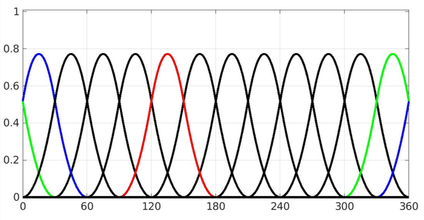
\includegraphics{fig/bsplines.png}

\textbf{Reading}

Tutorial on Splines by Samuel Jackson (click here).

Intro to Splines (click here).

\hypertarget{overview-2}{%
\subsection*{\texorpdfstring{\textbf{Overview}}{Overview}}\label{overview-2}}
\addcontentsline{toc}{subsection}{\textbf{Overview}}

In this module, you will learn \textbf{Basis expansions and parametric
splines}, flexible extensions of linear regression that enable modeling
complex, non-linear relationships between predictors and the response
variable.

\textbf{After completing this module, you will understand:}

\begin{itemize}
\item
  Basis Functions and knots
\item
  Piecewise Linear Splines
\item
  Piecewise Cubic Splines
\item
  Bias-Variance Tradeoff
\item
  Criteria for model prediction performance (CV, GCV, AIC).
\end{itemize}

\hypertarget{motivation-and-examples-7}{%
\subsection*{Motivation and Examples}\label{motivation-and-examples-7}}
\addcontentsline{toc}{subsection}{Motivation and Examples}

\begin{tcolorbox}[enhanced jigsaw, breakable, colbacktitle=quarto-callout-important-color!10!white, left=2mm, colframe=quarto-callout-important-color-frame, opacityback=0, coltitle=black, colback=white, rightrule=.15mm, title=\textcolor{quarto-callout-important-color}{\faExclamation}\hspace{0.5em}{Motivation:}, titlerule=0mm, opacitybacktitle=0.6, leftrule=.75mm, toprule=.15mm, arc=.35mm, bottomtitle=1mm, toptitle=1mm, bottomrule=.15mm]

Linear regression assumes a linear relationship between predictors and
the response. However, real-world data often exhibit \textbf{non-linear
patterns} that cannot be captured well by straight lines.

\begin{itemize}
\tightlist
\item
  \textbf{Basis expansions} allow us to transform predictors using
  functions (e.g., polynomials) to model non-linear relationships.
\item
  \textbf{Parametric splines} provide even more flexibility by fitting
  piecewise polynomials that are smooth at points called knots.
\end{itemize}

Using these methods helps avoid mis-specifying the functional form of
the model, leading to \textbf{more accurate fits}, \textbf{better
predictions}, and \textbf{valid inference}.

\end{tcolorbox}

\textbf{Motivating Example: Birthweight and Mothers Age} In a 2023 study
of low birth weight among infants in Georgia, data were collected for
\(N = 5{,}000\) infants. Gestational age (in weeks) and maternal age
were recorded to assess the relationship between gestational age and
infant birthweight (in grams). The dataset includes the following
variables:

\begin{itemize}
\item
  \(gw\) : gestational age in weeks.
\item
  \(age\): maternal age at delivery
\item
  \(bw\) birthweight at delivery in grams
\end{itemize}


\includegraphics{Module_4A_Splines_files/figure-pdf/unnamed-chunk-2-1.pdf}

\begin{itemize}
\tightlist
\item
  We see a non-linear relationship between \(gw\) and \(bw\) of a
  newborn.
\end{itemize}

\begin{center}\rule{0.5\linewidth}{0.5pt}\end{center}

\hypertarget{why-not-linear-regression-the-wrong-approach-1}{%
\subsubsection*{\texorpdfstring{Why Not linear regression?
\ul{\textbf{The wrong
approach}}}{Why Not linear regression? The wrong approach}}\label{why-not-linear-regression-the-wrong-approach-1}}
\addcontentsline{toc}{subsubsection}{Why Not linear regression?
\ul{\textbf{The wrong approach}}}

Let's fit a linear regression model as a baseline to assess how well it
captures this relationship. We'll then compare it to more flexible
approaches, such as basis expansions or splines, to see if they provide
a better fit.

\begin{verbatim}

Call:
lm(formula = bw ~ gw, data = dat)

Residuals:
    Min      1Q  Median      3Q     Max 
-761.50  -83.01   16.80  100.80  348.80 

Coefficients:
             Estimate Std. Error t value Pr(>|t|)    
(Intercept) -2177.513     39.351  -55.34   <2e-16 ***
gw            141.808      1.019  139.10   <2e-16 ***
---
Signif. codes:  0 '***' 0.001 '**' 0.01 '*' 0.05 '.' 0.1 ' ' 1

Residual standard error: 144.2 on 4998 degrees of freedom
Multiple R-squared:  0.7947,    Adjusted R-squared:  0.7947 
F-statistic: 1.935e+04 on 1 and 4998 DF,  p-value: < 2.2e-16
\end{verbatim}


\includegraphics{Module_4A_Splines_files/figure-pdf/unnamed-chunk-3-1.pdf}

\begin{itemize}
\item
  The linear fit does not capture the non-linear trend in the
  relationship between gestational age (\(gw\)) and birthweight
  (\(bw\)).
\item
  Overestimates birthweight at lower and higher gestational ages.
\item
  Doesn't capture curvature in the true relationship.
\item
  Suggests the need for a more flexible modeling approach, such as basis
  expansions or splines, to better capture the underlying structure.
\end{itemize}

\begin{center}\rule{0.5\linewidth}{0.5pt}\end{center}

\hypertarget{a-better-approach-basis-expansions-and-splines}{%
\subsection*{\texorpdfstring{\ul{A Better Approach: Basis Expansions and
Splines}}{A Better Approach: Basis Expansions and Splines}}\label{a-better-approach-basis-expansions-and-splines}}
\addcontentsline{toc}{subsection}{\ul{A Better Approach: Basis
Expansions and Splines}}

\textbf{\textcolor{blue}{Basis Expansion}}

\begin{itemize}
\tightlist
\item
  Consider the regression model:
\end{itemize}

\[
y_i = g(x_i) + \epsilon_i,
\]

where \(g(x_i)\) represents the true, possibly non-linear relationship
between the predictor \(x_i\) and the response \(y_i\), and
\(\epsilon_i\) is the error term.

\begin{itemize}
\tightlist
\item
  One common approach is to express \(g(x_i)\) as a linear combination
  of \(M\) known basis functions \(b_m(x_i)\):
\end{itemize}

\[
g(x_i) = \sum_{m=1}^M \beta_m b_m(x_i),
\]

where \(\beta_m\) are unknown coefficients to be estimated.

\begin{itemize}
\item
  \(b_m(x_i)\) are called \textbf{Basis Function} and are chosen and
  fixed \textbf{a priori}, serving as known transformations of the
  original predictor \(x_i\).
\item
  Our task is to estimate the coefficients \(\beta_m\) corresponding to
  these transformed variables.
\item
  Basis functions provide a flexible framework to model complex,
  non-linear relationships by representing \(g(x)\) as a combination of
  simpler functions. They are fundamental tools in functional data
  analysis and optimization, enabling the modeling of curves as
  piecewise or smoothly varying functions.
\end{itemize}

Below are some common examples of Basis Functions:

\begin{tcolorbox}[enhanced jigsaw, rightrule=.15mm, breakable, left=2mm, colframe=quarto-callout-tip-color-frame, opacityback=0, leftrule=.75mm, toprule=.15mm, colback=white, arc=.35mm, bottomrule=.15mm]

\textbf{1. \textbf{Polynomial Basis}}\vspace{2mm}

\textbf{Definition:} A polynomial basis uses powers of the predictor
variable to model non-linear trends. The basis functions are:

\[
b_1(x) = 1,\quad b_2(x) = x,\quad b_3(x) = x^2,\quad \ldots,\quad b_M(x) = x^{M-1}
\]

\textbf{Model:}

\[
g(x) = \beta_0 + \beta_1 x + \beta_2 x^2 + \cdots + \beta_{M-1} x^{M-1}
\]

\textbf{Use Case:} Polynomial bases are useful when the underlying
relationship is smooth and continuous, such as quadratic or cubic
trends. However, high-degree polynomials can lead to
\textbf{overfitting} and \textbf{numerical instability}, especially near
the boundaries (Runge's phenomenon).

\end{tcolorbox}

\begin{tcolorbox}[enhanced jigsaw, rightrule=.15mm, breakable, left=2mm, colframe=quarto-callout-tip-color-frame, opacityback=0, leftrule=.75mm, toprule=.15mm, colback=white, arc=.35mm, bottomrule=.15mm]

\textbf{2. \textbf{Indicator Basis (Step Functions)}}\vspace{2mm}

\textbf{Definition:} An indicator basis partitions the domain of ( x )
into intervals and defines a separate basis function for each interval:

\[
b_m(x) = 
\begin{cases}
1 & \text{if } x \in I_m \\
0 & \text{otherwise}
\end{cases}
\]

where ( I\_m ) is the ( m\^{}\text{th} ) interval.

\textbf{Model:}

\[
g(x) = \sum_{m=1}^M \beta_m \cdot \mathbb{1}_{\{x \in I_m\}}
\]

\textbf{Use Case:} This approach is useful for \textbf{piecewise
constant} modeling, especially when the data exhibit abrupt changes or
discontinuities. However, the resulting model is not smooth, and
predictions can jump sharply at the boundaries between intervals.

\end{tcolorbox}

\begin{tcolorbox}[enhanced jigsaw, rightrule=.15mm, breakable, left=2mm, colframe=quarto-callout-tip-color-frame, opacityback=0, leftrule=.75mm, toprule=.15mm, colback=white, arc=.35mm, bottomrule=.15mm]

\textbf{3. \textbf{Periodic Basis (Fourier Series)}}\vspace{2mm}

\textbf{Definition:} Periodic bases use sine and cosine functions to
capture repeating patterns in the data. A typical Fourier basis includes
terms like:

\[
b_1(x) = \sin(2\pi x),\quad b_2(x) = \cos(2\pi x),\quad b_3(x) = \sin(4\pi x),\quad \ldots
\]

\textbf{Model:}

\[
g(x) = \beta_1 \sin(2\pi x) + \beta_2 \cos(2\pi x) + \cdots
\]

\textbf{Use Case:} Periodic bases are ideal for \textbf{cyclical data},
such as seasonal trends (e.g., monthly temperatures, daily traffic
volume). They provide a smooth, continuous fit and naturally model data
that repeat over a fixed period.

\end{tcolorbox}

\hypertarget{summary-table-of-basis-function-types}{%
\subsection*{Summary Table of Basis Function
Types}\label{summary-table-of-basis-function-types}}
\addcontentsline{toc}{subsection}{Summary Table of Basis Function Types}

\begin{longtable}[]{@{}
  >{\raggedright\arraybackslash}p{(\columnwidth - 6\tabcolsep) * \real{0.2500}}
  >{\raggedright\arraybackslash}p{(\columnwidth - 6\tabcolsep) * \real{0.2500}}
  >{\raggedright\arraybackslash}p{(\columnwidth - 6\tabcolsep) * \real{0.2500}}
  >{\raggedright\arraybackslash}p{(\columnwidth - 6\tabcolsep) * \real{0.2500}}@{}}
\toprule\noalign{}
\begin{minipage}[b]{\linewidth}\raggedright
Basis Type
\end{minipage} & \begin{minipage}[b]{\linewidth}\raggedright
Captures
\end{minipage} & \begin{minipage}[b]{\linewidth}\raggedright
Smoothness
\end{minipage} & \begin{minipage}[b]{\linewidth}\raggedright
Use Case
\end{minipage} \\
\midrule\noalign{}
\endhead
\bottomrule\noalign{}
\endlastfoot
Polynomial & Global smooth trends & Smooth & Curved but continuous
relationships \\
Indicator & Piecewise constant & Discontinuous & Sharp jumps or
categorization \\
Periodic & Cyclical/repeating trends & Smooth & Seasonal or periodic
data \\
\end{longtable}

\begin{center}\rule{0.5\linewidth}{0.5pt}\end{center}

\hypertarget{polynomial-regression}{%
\subsection*{Polynomial Regression}\label{polynomial-regression}}
\addcontentsline{toc}{subsection}{Polynomial Regression}

Let's fit a \ul{Polynomial Regression} to the birthweight outcomes:

\[
\begin{align*}
\text{Quadratic } y_i & = \beta_0 + \beta_1 x_i + \beta_2 x_i^2 + e_i\\
\text{Cubic } y_i & = \beta_0 + \beta_1 x_i + \beta_2 x_i^2 +  \beta_3 x_i^3 + e_i\\
\end{align*}
\]


\includegraphics{Module_4A_Splines_files/figure-pdf/unnamed-chunk-4-1.pdf}

The \textbf{linear} model provides a general upward trend, but it fails
to capture subtle curvature in the data, particularly at the extremes of
gestational age. The \textbf{quadratic} model improves the fit by
introducing curvature, better capturing the accelerating increase in
birthweight with gestational age. However, it tends to oversimplify the
relationship near the boundaries. The \textbf{cubic} model offers the
most flexible fit among the three, capturing inflection points and more
nuanced trends in the data. While it improves predictive accuracy,
especially in the mid-gestational range, it also may introduce slight
overfitting near the edges. Overall, higher-degree polynomials offer
more flexibility but must be used cautiously to avoid instability and
overfitting, particularly with extrapolation.

Note that all polynomial functions often cannot model the ends very
well.

\begin{center}\rule{0.5\linewidth}{0.5pt}\end{center}

\hypertarget{fitting-a-polynomial-regression-in-r}{%
\subsection*{Fitting a Polynomial Regression in
R}\label{fitting-a-polynomial-regression-in-r}}
\addcontentsline{toc}{subsection}{Fitting a Polynomial Regression in R}

\begin{Shaded}
\begin{Highlighting}[]
\CommentTok{\#Quadratic polynomial model}
\NormalTok{fit2 }\OtherTok{\textless{}{-}} \FunctionTok{lm}\NormalTok{(bw }\SpecialCharTok{\textasciitilde{}}\NormalTok{ gw }\SpecialCharTok{+} \FunctionTok{I}\NormalTok{(gw}\SpecialCharTok{\^{}}\DecValTok{2}\NormalTok{), }\AttributeTok{data =}\NormalTok{ dat)}

\CommentTok{\#Cubic polynomial model}
\NormalTok{fit3 }\OtherTok{\textless{}{-}} \FunctionTok{lm}\NormalTok{(bw }\SpecialCharTok{\textasciitilde{}}\NormalTok{ gw }\SpecialCharTok{+} \FunctionTok{I}\NormalTok{(gw}\SpecialCharTok{\^{}}\DecValTok{2}\NormalTok{) }\SpecialCharTok{+} \FunctionTok{I}\NormalTok{(gw}\SpecialCharTok{\^{}}\DecValTok{3}\NormalTok{), }\AttributeTok{data =}\NormalTok{ dat)}
\end{Highlighting}
\end{Shaded}

\begin{longtable}[]{@{}
  >{\raggedright\arraybackslash}p{(\columnwidth - 4\tabcolsep) * \real{0.3333}}
  >{\raggedright\arraybackslash}p{(\columnwidth - 4\tabcolsep) * \real{0.3333}}
  >{\raggedright\arraybackslash}p{(\columnwidth - 4\tabcolsep) * \real{0.3333}}@{}}
\toprule\noalign{}
\begin{minipage}[b]{\linewidth}\raggedright
Metric
\end{minipage} & \begin{minipage}[b]{\linewidth}\raggedright
Quadratic Model (\texttt{fit2})
\end{minipage} & \begin{minipage}[b]{\linewidth}\raggedright
Cubic Model (\texttt{fit3})
\end{minipage} \\
\midrule\noalign{}
\endhead
\bottomrule\noalign{}
\endlastfoot
\textbf{Model formula} & \( bw \sim gw + gw^2 \) &
\( bw \sim gw + gw^2 + gw^3 \) \\
\textbf{Residual standard error} & 113.8 & 110.1 \\
\textbf{Adjusted ( R\^{}2 )} & 0.872 & 0.880 \\
\textbf{F-statistic} & 17,030 (p \textless{} 2.2e-16) & 12,240 (p
\textless{} 2.2e-16) \\
\textbf{Coefficient significance} & All terms highly significant (p
\textless{} 2e-16) & All terms highly significant (p \textless{}
2e-16) \\
\textbf{Max residual} & 451.45 & 300.81 \\
\textbf{Interpretation of coefficients} & Negative quadratic term
indicates decreasing marginal effect of gestational weeks on birthweight
& Cubic term allows more flexible curvature capturing subtle
inflections \\
\end{longtable}

\begin{itemize}
\item
  Both quadratic and cubic models explain a large proportion of variance
  in birthweight, with adjusted \(R^2\) above 0.87.
\item
  The cubic model shows a modest improvement over quadratic:

  \begin{itemize}
  \tightlist
  \item
    Lower residual standard error (110.1 vs 113.8)
  \item
    Slightly higher adjusted \(R^2\) (0.880 vs 0.872)
  \item
    Smaller maximum residuals (300.81 vs 451.45)
  \end{itemize}
\item
  All polynomial terms are highly statistically significant, confirming
  nonlinear relationships between gestational age and birthweight.
\item
  The cubic term adds flexibility, capturing subtle curvature and
  inflection points missed by the quadratic model.
\item
  However, the improvement is modest and higher-degree polynomials risk
  overfitting.
\end{itemize}

\begin{center}\rule{0.5\linewidth}{0.5pt}\end{center}

\hypertarget{piecewise-regression}{%
\section*{Piecewise Regression}\label{piecewise-regression}}
\addcontentsline{toc}{section}{Piecewise Regression}

\markright{Piecewise Regression}

One intuitive approach to modeling \textbf{non-linear relationships}
between a predictor and the response is to divide the range of the
predictor into several \textbf{meaningful subregions}. For example,
consider pregnancy length as a predictor:

\begin{itemize}
\tightlist
\item
  \textbf{Preterm:} less than 37 weeks\\
\item
  \textbf{Full-term:} 37 to 41 weeks\\
\item
  \textbf{Post-term:} more than 42 weeks
\end{itemize}

Rather than fitting a single global polynomial across the entire range,
we can model the relationship using polynomial functions
\textcolor{blue}{separately within each region}. This technique allows
for greater flexibility and can better capture local patterns in the
data without overfitting globally.

The values that define the boundaries between these regions---such as 37
and 42 weeks in the example above---are called \textcolor{blue}{knots}.

\textbf{Knots} are central to methods such as piecewise regression,
where the domain of the predictor is split at these points, and separate
(yet smoothly connected) polynomial functions are fit in each subregion.
This structure enables models to adapt to changes in the shape of the
data while preserving continuity and smoothness.

Piecewise regression can be interpreted as a model in which the basis
functions of \(x_i\) are allowed to interact with indicator (dummy)
variables that define distinct regions of the predictor's domain. For
example:

where

\[
D_{1i} =
\begin{cases}
1 & 37 \leq x_i < 42\\
0 & OW
\end{cases}
\]

\[
D_{2i} =
\begin{cases}
1 &  x_i \geq 42\\
0 & OW
\end{cases}
\]

We have two cut-points (knots) which yields three regions. We only need
two dummy variables for three regions.

The piecewise quadratic regression model is expressed as:

\[
\begin{aligned}
y_i =\ & \beta_0 + \beta_1 x_i + \beta_2 x_i^2 & \text{(Preterm baseline)} \\
& + \beta_3 D_{1i} + \beta_4 x_i D_{1i} + \beta_5 x_i^2 D_{1i} & \text{(Full-term adjustment)} \\
& + \beta_6 D_{2i} + \beta_7 x_i D_{2i} + \beta_8 x_i^2 D_{2i} & \text{(Post-term adjustment)}\\
& + \epsilon
\end{aligned}
\]

\begin{center}\rule{0.5\linewidth}{0.5pt}\end{center}

\hypertarget{fitting-piecewise-polynomial-regression-models-in-r}{%
\subsection*{Fitting Piecewise Polynomial Regression Models in
R}\label{fitting-piecewise-polynomial-regression-models-in-r}}
\addcontentsline{toc}{subsection}{Fitting Piecewise Polynomial
Regression Models in R}

In this section, we demonstrate how to fit piecewise polynomial
regression models by dividing the predictor variable --- gestational
weeks (\(gw\)) --- into meaningful regions defined above and fitting
separate polynomial models within each region. We use indicator
variables for the regions and interact them with polynomial terms of
\(gw\).

We divide the gestational weeks into three regions based on clinical
definitions:

\begin{itemize}
\tightlist
\item
  \textbf{Preterm:} \(gw < 37\) weeks\\
\item
  \textbf{Full-term:} \(37 \leq gw \leq 41\) weeks\\
\item
  \textbf{Post-term:} \(gw \geq 42\) weeks
\end{itemize}

In R, we create logical vectors to indicate these regions:

\begin{Shaded}
\begin{Highlighting}[]
\NormalTok{Ind1 }\OtherTok{=}\NormalTok{ dat}\SpecialCharTok{$}\NormalTok{gw }\SpecialCharTok{\textgreater{}=} \DecValTok{37} \SpecialCharTok{\&}\NormalTok{ dat}\SpecialCharTok{$}\NormalTok{gw }\SpecialCharTok{\textless{}=} \DecValTok{41} \CommentTok{\#Full term indicator}
\NormalTok{Ind2 }\OtherTok{=}\NormalTok{ dat}\SpecialCharTok{$}\NormalTok{gw }\SpecialCharTok{\textgreater{}=} \DecValTok{42}                \CommentTok{\#Post{-}term indicator}
\end{Highlighting}
\end{Shaded}

The preterm region is implicitly defined where both \texttt{Ind1} and
\texttt{Ind2} are FALSE.

To model non-linear relationships between birthweight (\texttt{bw}) and
gestational weeks (\texttt{gw}) that may vary across different
gestational age regions (e.g., preterm, full-term, post-term), we may
extend the model to include quadratic terms for \texttt{gw}.

The piecewise quadratic regression model with interaction terms can be
written as:

\[
bw_i = \beta_0 + \beta_1 gw_i + \beta_2 gw_i^2 + \beta_3 Ind1_i + \beta_4 Ind2_i + \beta_5 (gw_i \times Ind1_i) + \beta_6 (gw_i \times Ind2_i) + \beta_7 (gw_i^2 \times Ind1_i) + \beta_8 (gw_i^2 \times Ind2_i) + \epsilon_i
\]

This model allows both the intercept and the linear and quadratic
effects of gestational weeks to vary across the three gestational age
regions. This flexibility enables better modeling of complex,
region-specific relationships between gestational age and birthweight.

\begin{Shaded}
\begin{Highlighting}[]
\NormalTok{fit5 }\OtherTok{=} \FunctionTok{lm}\NormalTok{ (bw}\SpecialCharTok{\textasciitilde{}}\NormalTok{(gw }\SpecialCharTok{+} \FunctionTok{I}\NormalTok{(gw}\SpecialCharTok{\^{}}\DecValTok{2}\NormalTok{))}\SpecialCharTok{*}\NormalTok{(Ind1}\SpecialCharTok{+}\NormalTok{ Ind2), }\AttributeTok{data =}\NormalTok{ dat)}

\DocumentationTok{\#\#\#Important}
\CommentTok{\# In R formulas, the caret symbol (\^{}) is not interpreted as exponentiation but as a formula operator indicating interactions or polynomial expansions of terms.}
\CommentTok{\# }
\CommentTok{\# Writing (gw\^{}2) without wrapping it in the I() function causes R to treat it as "gw to the power of 2" in the formula sense (interactions), not as the squared variable $gw\^{}2$.}
\CommentTok{\# }
\CommentTok{\# This leads to an unintended model structure that does not include the quadratic term properly, and may result in errors or nonsensical coefficients.}
\NormalTok{dontdothis }\OtherTok{=} \FunctionTok{lm}\NormalTok{(bw}\SpecialCharTok{\textasciitilde{}}\NormalTok{(gw}\SpecialCharTok{+}\NormalTok{(gw}\SpecialCharTok{\^{}}\DecValTok{2}\NormalTok{))}\SpecialCharTok{*}\NormalTok{(Ind1}\SpecialCharTok{+}\NormalTok{ Ind2), }\AttributeTok{data =}\NormalTok{ dat)}

\NormalTok{fit6 }\OtherTok{=} \FunctionTok{lm}\NormalTok{ (bw}\SpecialCharTok{\textasciitilde{}}\NormalTok{(gw}\SpecialCharTok{+}\FunctionTok{I}\NormalTok{(gw}\SpecialCharTok{\^{}}\DecValTok{2}\NormalTok{) }\SpecialCharTok{+} \FunctionTok{I}\NormalTok{(gw}\SpecialCharTok{\^{}}\DecValTok{3}\NormalTok{))}\SpecialCharTok{*}\NormalTok{(Ind1}\SpecialCharTok{+}\NormalTok{ Ind2), }\AttributeTok{data =}\NormalTok{ dat)}
\end{Highlighting}
\end{Shaded}


\includegraphics{Module_4A_Splines_files/figure-pdf/unnamed-chunk-9-1.pdf}

\textbf{Limitations in Piecewise Polynomials:}

\begin{itemize}
\item
  Limited flexibility in capturing complex trends: Although polynomial
  fits (linear, quadratic, cubic) are applied separately in each region,
  they often produce similar shapes, which may fail to represent subtle
  changes in the relationship between gestational age and
  birthweight---especially where the effect weakens at higher
  gestational weeks.
\item
  Lack of smoothness at knots: The fitted curves generally do not join
  smoothly at the boundaries (knots) between regions. This can cause
  abrupt changes or discontinuities in the predicted values or their
  slopes, which is unrealistic for most natural processes.
\item
  High model complexity: Fitting separate polynomials for each region
  requires estimating many parameters, increasing the degrees of freedom
  and the potential for overfitting, particularly with limited data.
\end{itemize}

\begin{center}\rule{0.5\linewidth}{0.5pt}\end{center}

\hypertarget{discontinuities-at-the-boundaries}{%
\subsection*{Discontinuities at the
Boundaries}\label{discontinuities-at-the-boundaries}}
\addcontentsline{toc}{subsection}{Discontinuities at the Boundaries}

Piecewise polynomial regression fits separate polynomial models within
different intervals of the predictor variable separated by \emph{knots}.
While this allows for flexible modeling of nonlinear relationships, an
important drawback is the potential for \textbf{discontinuities} at
these knot points.

\ul{\textbf{What is a discontinuity?}} A discontinuity occurs when the
fitted function or its derivatives have abrupt changes at the knot
locations. For example, suppose the predictor \(x\) is divided into two
regions by a knot at \(k\). We fit two separate polynomial functions:

\[
g_1(x) = \beta_0^{(1)} + \beta_1^{(1)} x + \beta_2^{(1)} x^2, \quad x < k
\]

\[
g_2(x) = \beta_0^{(2)} + \beta_1^{(2)} x + \beta_2^{(2)} x^2, \quad x \geq k
\]

If these functions are not constrained to be equal at \(x = k\), then
the value of \(g_1(k)\) may differ from \(g_2(k)\), causing a
\textbf{jump} in the predicted curve.

\begin{enumerate}
\def\labelenumi{\arabic{enumi}.}
\tightlist
\item
  \ul{\textbf{Discontinuity in the function:}} If
  \(g_1(k) \neq g_2(k)\), the function is \textbf{discontinuous} at
  \(k\). This means the predicted response suddenly changes as we cross
  the knot, which is usually unrealistic for continuous processes like
  birthweight increasing with gestational age.
\item
  \ul{\textbf{Discontinuity in derivatives:}} Even if
  \(g_1(k) = g_2(k)\), the slope or curvature may still jump,e.g.,
\end{enumerate}

\begin{itemize}
\item
  If \(g_1'(k) \neq g_2'(k)\), the first derivative (slope) is
  discontinuous.
\item
  If \(g_1''(k) \neq g_2''(k)\), the second derivative (curvature) is
  discontinuous.
\end{itemize}

Discontinuities in derivatives make the fitted curve look ``kinked'' or
less smooth at the knots.

\ul{\textbf{Why does this matter?}} Discontinuities reduce the
\textbf{smoothness} of the regression curve. For biological or physical
processes, smooth transitions are often expected.Piecewise polynomial
regression without additional constraints does \textbf{not guarantee
continuity or smoothness} at the knots.

\begin{center}\rule{0.5\linewidth}{0.5pt}\end{center}

\hypertarget{section-22}{%
\section*{\texorpdfstring{\textcolor{purple}{Summary}}{}}\label{section-22}}
\addcontentsline{toc}{section}{\textcolor{purple}{Summary}}

\markright{\textcolor{purple}{Summary}}

\begin{longtable}[]{@{}
  >{\raggedright\arraybackslash}p{(\columnwidth - 2\tabcolsep) * \real{0.5000}}
  >{\raggedright\arraybackslash}p{(\columnwidth - 2\tabcolsep) * \real{0.5000}}@{}}
\toprule\noalign{}
\begin{minipage}[b]{\linewidth}\raggedright
\textbf{Section}
\end{minipage} & \begin{minipage}[b]{\linewidth}\raggedright
\textbf{Description}
\end{minipage} \\
\midrule\noalign{}
\endhead
\bottomrule\noalign{}
\endlastfoot
\textbf{What is the Model?} & A \textbf{basis expansion model} expresses
an unknown function \(g(x)\) as a linear combination of known basis
functions: \(g(x_i) = \sum_{m=1}^M \beta_m b_m(x_i)\) The goal is to
flexibly model nonlinear relationships by choosing appropriate basis
functions \(b_m(\cdot)\). \\
\textbf{Polynomial Basis} & Uses powers of \(x\) as basis functions:
\(b_1(x) = 1, \quad b_2(x) = x, \quad b_3(x) = x^2, \quad \ldots, \quad b_M(x) = x^{M-1}\)
Leads to polynomial regression models like quadratic or cubic
regression. \\
\textbf{Piecewise Polynomial Basis} & Divides the domain of \(x\) into
intervals with \textbf{knots} and fits separate polynomials on each
interval. Uses indicator functions \(D_i\) to select intervals, e.g.,
\(y_i = \beta_0 + \beta_1 x_i + \beta_2 x_i^2 + \beta_3 D_{1i} + \beta_4 x_i D_{1i} + \ldots\) \\
\textbf{Indicator Variables (Knots)} & \(D_{1i}, D_{2i}, \ldots\) are
defined to indicate which interval \(x_i\) belongs to, enabling
piecewise definitions of the function. E.g., \(D_{1i} = 1\) if \(x_i\)
in interval 1, else 0. Allows flexibility but can cause discontinuities
at knots if not constrained. \\
\textbf{Parametric Splines} & Piecewise polynomials with constraints
(e.g., continuity, smoothness) at knots to avoid jumps or sharp corners.
Ensures the function and its derivatives match at knots, yielding smooth
curves useful in regression and smoothing applications. \\
\textbf{Why Use Basis Expansions?} & To model \textbf{nonlinear} effects
in regression flexibly while retaining a linear structure in parameters
\(\beta_m\), enabling standard estimation methods like least squares.
Basis expansions allow balancing flexibility and interpretability. \\
\textbf{Key R Modeling Note} & In R formulas, polynomial terms like
\(x^2\) must be wrapped in \texttt{I()} to indicate arithmetic, e.g.,
\texttt{I(x\^{}2)}, otherwise caret \texttt{\^{}} is interpreted as
formula syntax (e.g., interaction). \\
\textbf{Continuity and Smoothness} & Without constraints, piecewise
polynomials can be \textbf{discontinuous} or have sharp corners at
knots. Parametric splines enforce conditions so that the function is
continuous and smooth (derivatives continuous) across knots, improving
fit quality and interpretability. \\
\end{longtable}

\bookmarksetup{startatroot}

\hypertarget{module-4b-parametric-splines}{%
\chapter*{Module 4B Parametric
Splines}\label{module-4b-parametric-splines}}
\addcontentsline{toc}{chapter}{Module 4B Parametric Splines}

\markboth{Module 4B Parametric Splines}{Module 4B Parametric Splines}

\begin{figure}

{\centering 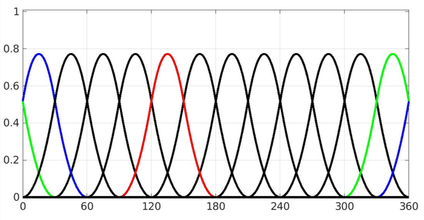
\includegraphics{fig/bsplines.png}

}

\end{figure}

\hypertarget{motivation-and-examples-8}{%
\subsection*{Motivation and Examples}\label{motivation-and-examples-8}}
\addcontentsline{toc}{subsection}{Motivation and Examples}

\begin{tcolorbox}[enhanced jigsaw, breakable, colbacktitle=quarto-callout-important-color!10!white, left=2mm, colframe=quarto-callout-important-color-frame, opacityback=0, coltitle=black, colback=white, rightrule=.15mm, title=\textcolor{quarto-callout-important-color}{\faExclamation}\hspace{0.5em}{Motivation:}, titlerule=0mm, opacitybacktitle=0.6, leftrule=.75mm, toprule=.15mm, arc=.35mm, bottomtitle=1mm, toptitle=1mm, bottomrule=.15mm]

So far, we have explored \textbf{Basis Expansion} in approaches such as
polynomial regression and piecewise regression, where the response
variable is divided into subregions and modeled separately with
different polynomial functions.

\textcolor{blue}{Basis expansion is the overall process of transforming your predictors by expanding them into these basis functions.}

However, piecewise regression has some key limitations:

\begin{itemize}
\tightlist
\item
  It offers limited flexibility in capturing complex patterns.\\
\item
  The fitted curves often lack smoothness at the knot points where the
  pieces meet.\\
\item
  It can lead to models with high complexity and many parameters.
\end{itemize}

To address these issues, we now introduce \textbf{parametric splines}.

\textbf{Parametric splines} extend this idea by fitting piecewise
polynomial functions that are smoothly connected at specified points
called \textbf{knots}.

These approaches help us avoid mis-specifying the model's functional
form, resulting in \textbf{more accurate fits}, \textbf{improved
predictions}, and \textbf{valid statistical inference}, all while
respecting the assumptions of linear regression.

\end{tcolorbox}

\begin{center}\rule{0.5\linewidth}{0.5pt}\end{center}

\hypertarget{introduction-to-splines}{%
\section*{Introduction to Splines}\label{introduction-to-splines}}
\addcontentsline{toc}{section}{Introduction to Splines}

\markright{Introduction to Splines}

Splines are a powerful class of functions used to model complex,
non-linear relationships by joining piecewise polynomial segments in a
smooth way. Unlike simple piecewise regression, splines ensure
continuity and smoothness at the \textbf{knots}.

\hypertarget{general-form-of-a-polynomial-spline-model}{%
\subsection*{General Form of a Polynomial Spline
Model}\label{general-form-of-a-polynomial-spline-model}}
\addcontentsline{toc}{subsection}{General Form of a Polynomial Spline
Model}

A \textbf{polynomial spline} is a flexible modeling tool used to
represent non-linear relationships. It constructs the regression
function by piecing together polynomial functions that are joined at
specific values of the predictor variable, known as \textbf{knots}.

The general form of a degree-\(d\) polynomial spline with \(M\) knots
\(k_1, k_2, \dots, k_M\) is:

\[
y_i = \beta_0 + \sum_{j=1}^d \beta_j x_i^j + \sum_{m=1}^M \gamma_m (x_i - k_m)^d_{+}
\]

where:

\begin{itemize}
\tightlist
\item
  \(d\) is the degree of the spline (e.g., 1 = linear, 2 = quadratic, 3
  = cubic),
\item
  \(k_m\) are the \textbf{knots}, where the segments of the spline are
  joined,
\item
  \((x_i - k_m)^d_{+} = \begin{cases}(x_i - k_m)^d & \text{if } x_i > k_m \\ 0 & \text{otherwise} \end{cases}\)
  is the \textbf{truncated power function},
\item
  \(\beta_j\) and \(\gamma_m\) are coefficients estimated from the data.
\end{itemize}

This is referred to as the \textcolor{blue}{truncated power basis}.

This form allows the spline to behave like a polynomial within each
region defined by the knots, but with flexibility to change shape at
each knot, while maintaining smoothness across the entire domain.

\hypertarget{polynomial-spline-examples}{%
\subsubsection*{Polynomial Spline
Examples}\label{polynomial-spline-examples}}
\addcontentsline{toc}{subsubsection}{Polynomial Spline Examples}

\begin{tcolorbox}[enhanced jigsaw, rightrule=.15mm, breakable, left=2mm, colframe=quarto-callout-tip-color-frame, opacityback=0, leftrule=.75mm, toprule=.15mm, colback=white, arc=.35mm, bottomrule=.15mm]

\begin{itemize}
\item
  \textbf{Linear spline} (\(d = 1\)):

  \[
  y_i = \beta_0 + \beta_1 x_i + \sum_{m=1}^M \gamma_m (x_i - k_m)_{+}
  \]

  \begin{itemize}
  \tightlist
  \item
    Continuous at the knots, but the \textbf{slope is not smooth} ---
    the first derivative is discontinuous.
  \item
    Each \(\gamma_m\) represents the \textbf{change in slope} at knot
    \(k_m\).
  \end{itemize}
\item
  \textbf{Quadratic spline} (\(d = 2\)):

  \[
  y_i = \beta_0 + \beta_1 x_i + \beta_2 x_i^2 + \sum_{m=1}^M \gamma_m (x_i - k_m)^2_{+}
  \]

  \begin{itemize}
  \tightlist
  \item
    Ensures the function and its \textbf{first derivative are
    continuous} at the knots.
  \end{itemize}
\item
  \textbf{Cubic spline} (\(d = 3\)):

  \[
  y_i = \beta_0 + \beta_1 x_i + \beta_2 x_i^2 + \beta_3 x_i^3 + \sum_{m=1}^M \gamma_m (x_i - k_m)^3_{+}
  \]

  \begin{itemize}
  \tightlist
  \item
    Ensures continuity of the:

    \begin{itemize}
    \tightlist
    \item
      Function itself,
    \item
      \textbf{First derivative} (slope),
    \item
      \textbf{Second derivative} (curvature).
    \end{itemize}
  \end{itemize}
\end{itemize}

\end{tcolorbox}

\hypertarget{practical-considerations}{%
\subsubsection*{Practical
Considerations}\label{practical-considerations}}
\addcontentsline{toc}{subsubsection}{Practical Considerations}

\begin{itemize}
\tightlist
\item
  \textbf{Linear splines} are good for interpretability. You can explain
  the slope change at each knot.
\item
  \textbf{Cubic splines} are widely used for smooth fits. They provide
  excellent flexibility while maintaining a smooth shape.
\item
  For cubic splines, \textbf{individual coefficients are not typically
  interpreted} --- instead, we focus on the fitted curve.
\end{itemize}

\begin{center}\rule{0.5\linewidth}{0.5pt}\end{center}

\hypertarget{section-23}{%
\subsection*{\texorpdfstring{\textcolor{green}{Linear Splines}}{}}\label{section-23}}
\addcontentsline{toc}{subsection}{\textcolor{green}{Linear Splines}}

A linear piecewise spline at knot locations 37 and 42 is specified as:

\[
y_i  = \beta_0 + \beta_1 x_i + \beta_2 (x_i - 37)_{+} + \beta_3 (x_i - 42)_{+} + \epsilon_i 
\]

\begin{itemize}
\tightlist
\item
  For \(x_i<37\)
\end{itemize}

\[
y_i = \beta_0 + \beta_1 x_i
\]

\begin{itemize}
\tightlist
\item
  For \(37 \leq x_i < 42\)
\end{itemize}

\[
\begin{align*}
y_i & = \beta_0 + \beta_1 x_i + \beta_2 (x_i - 37)_+ \\
&=  (\beta_0 - \beta_2 * 37) + (\beta_1 + \beta_2) x_i
\end{align*}
\]

\begin{itemize}
\tightlist
\item
  For \(42 \geq x_i\)
\end{itemize}

\[
\begin{align*}
y_i & = \beta_0 + \beta_1 x_i + \beta_2 (x_i - 37)_+ + \beta_3 (x_i - 42)_+\\
& = (\beta_0 - 37\beta_2   - 42\beta_3) + (\beta_1 + \beta_2 + \beta_3) x_i
\end{align*}
\]

\begin{itemize}
\tightlist
\item
  \(\beta_2\) and \(\beta_3\) represent \ul{changes} in slope compared
  to the previous region.
\end{itemize}

Note here we only need 4 regression coefficients compared to 6 in the
model that does not force connections at knots.

\begin{Shaded}
\begin{Highlighting}[]
\FunctionTok{load}\NormalTok{(}\FunctionTok{paste0}\NormalTok{(}\FunctionTok{getwd}\NormalTok{(), }\StringTok{"/data/GAbirth.RDATA"}\NormalTok{))}
\CommentTok{\#Linear Splines}
\NormalTok{Sp1 }\OtherTok{=}\NormalTok{ (dat}\SpecialCharTok{$}\NormalTok{gw }\SpecialCharTok{{-}} \DecValTok{37}\NormalTok{) }\SpecialCharTok{*} \FunctionTok{as.numeric}\NormalTok{(dat}\SpecialCharTok{$}\NormalTok{gw }\SpecialCharTok{\textgreater{}=} \DecValTok{37}\NormalTok{)}
\NormalTok{Sp2 }\OtherTok{=}\NormalTok{ (dat}\SpecialCharTok{$}\NormalTok{gw }\SpecialCharTok{{-}} \DecValTok{42}\NormalTok{) }\SpecialCharTok{*} \FunctionTok{as.numeric}\NormalTok{(dat}\SpecialCharTok{$}\NormalTok{gw }\SpecialCharTok{\textgreater{}=} \DecValTok{42}\NormalTok{)}
\NormalTok{fit7 }\OtherTok{\textless{}{-}} \FunctionTok{lm}\NormalTok{(bw }\SpecialCharTok{\textasciitilde{}}\NormalTok{ gw }\SpecialCharTok{+}\NormalTok{ Sp1 }\SpecialCharTok{+}\NormalTok{ Sp2, }\AttributeTok{data =}\NormalTok{ dat)}
\end{Highlighting}
\end{Shaded}


\includegraphics{Module_4B_Splines_files/figure-pdf/unnamed-chunk-3-1.pdf}

\begin{verbatim}

Call:
lm(formula = bw ~ gw + Sp1 + Sp2, data = dat)

Residuals:
    Min      1Q  Median      3Q     Max 
-396.83  -75.83    3.03   79.50  324.84 

Coefficients:
             Estimate Std. Error t value Pr(>|t|)    
(Intercept) -4759.298     56.686  -83.96   <2e-16 ***
gw            214.589      1.563  137.25   <2e-16 ***
Sp1          -122.260      2.356  -51.88   <2e-16 ***
Sp2          -154.294     15.275  -10.10   <2e-16 ***
---
Signif. codes:  0 '***' 0.001 '**' 0.01 '*' 0.05 '.' 0.1 ' ' 1

Residual standard error: 112.8 on 4996 degrees of freedom
Multiple R-squared:  0.8743,    Adjusted R-squared:  0.8742 
F-statistic: 1.158e+04 on 3 and 4996 DF,  p-value: < 2.2e-16
\end{verbatim}

\textbf{Interpretation:}

\begin{itemize}
\item
  The model fits birthweight \texttt{bw} as a piecewise linear function
  of gestational week \texttt{gw} with knots at 37 and 42 weeks.
\item
  \textbf{Intercept (-4759.3):} The estimated birthweight when
  \texttt{gw\ =\ 0} (outside the observed range, mainly a baseline
  reference).
\item
  \textbf{Coefficient for \texttt{gw} (214.6):} For gestational weeks
  \textbf{before 37}, each additional week increases birthweight by
  approximately 214 grams.
\item
  \textbf{Coefficient for \texttt{Sp1} (-122.3):} After 37 weeks, the
  slope changes by \texttt{-122.3}, so the weekly increase in
  birthweight slows down to about \texttt{214.6\ -\ 122.3\ =\ 92.3}
  grams per week between 37 and 42 weeks.
\item
  \textbf{Coefficient for \texttt{Sp2} (-154.3):} After 42 weeks, the
  slope decreases further by 154.3, leading to a smaller or potentially
  negative increase in birthweight beyond this point.
\item
  \textbf{Model fit:}

  \begin{itemize}
  \tightlist
  \item
    Residual standard error of 113 grams indicates typical prediction
    errors around this value.\\
  \item
    Multiple \texttt{R\^{}2\ =\ 0.874} shows the model explains 87.4\%
    of the variance in birthweight, indicating a strong fit.
  \end{itemize}
\end{itemize}

\begin{center}\rule{0.5\linewidth}{0.5pt}\end{center}

\hypertarget{section-24}{%
\subsection*{\texorpdfstring{\textcolor{green}{Cubic Splines}}{}}\label{section-24}}
\addcontentsline{toc}{subsection}{\textcolor{green}{Cubic Splines}}

Linear splines fit piecewise linear functions joined at knots. They are
easy to interpret and continuous, but their slope (first derivative) is
not smooth at the knots, which can create sharp changes.

\textbf{Cubic splines} improve upon piecewise linear or quadratic models
by fitting \textbf{piecewise cubic polynomials} that are
\textbf{smoothly joined at the knots}. Specifically:

\begin{itemize}
\tightlist
\item
  The \textbf{function itself} is continuous at the knots.\\
\item
  The \textbf{first derivative} (i.e., the slope) is continuous,
  ensuring \textbf{no sharp changes in direction}.
  \textcolor{blue}{If the first derivative is not continuous at the knots, the slope can abruptly change—causing visible kinks or corners in the curve.}
\item
  The \textbf{second derivative} is also continuous, which ensures
  \textbf{smooth curvature} across the entire domain.
  \textcolor{blue}{If the second derivative is not continuous at a knot, the curve may still look smooth, but it will change curvature abruptly — like a bend that's not sharp, but still visually unnatural.}
\end{itemize}

This level of continuity results in a smooth, natural-looking curve
without abrupt bends or changes in slope. Because cubic splines ensure
smoothness up to the second derivative, they are commonly used for
modeling smooth nonlinear relationships.

The cubic spline with knots at \(\kappa_1\) and \(\kappa_2\) can be
written as:

\[
g(x_i) = \beta_0 + \beta_1 x_i + \beta_2 x_i^2 + \beta_3 x_i^3 + \beta_4 (x_i - \kappa_1)_+^3 + \beta_5 (x_i - \kappa_2)_+^3
\]

where

\[(x - \kappa)_+^3 =
\begin{cases}
  (x - \kappa)^3, & \text{if } x > \kappa, \\
  0, & \text{otherwise.}
\end{cases}\]

and \((\kappa_1, \kappa_2) = (37, 42)\).

\begin{Shaded}
\begin{Highlighting}[]
\CommentTok{\#Cubic Splines}
\NormalTok{Sp1 }\OtherTok{=}\NormalTok{ (dat}\SpecialCharTok{$}\NormalTok{gw }\SpecialCharTok{{-}} \DecValTok{37}\NormalTok{)}\SpecialCharTok{\^{}}\DecValTok{3}\SpecialCharTok{*}\FunctionTok{as.numeric}\NormalTok{(dat}\SpecialCharTok{$}\NormalTok{gw }\SpecialCharTok{\textgreater{}=} \DecValTok{37}\NormalTok{ )}
\NormalTok{Sp2 }\OtherTok{=}\NormalTok{ (dat}\SpecialCharTok{$}\NormalTok{gw }\SpecialCharTok{{-}} \DecValTok{42}\NormalTok{)}\SpecialCharTok{\^{}}\DecValTok{3}\SpecialCharTok{*}\FunctionTok{as.numeric}\NormalTok{(dat}\SpecialCharTok{$}\NormalTok{gw }\SpecialCharTok{\textgreater{}=} \DecValTok{42}\NormalTok{)}
\NormalTok{fit8 }\OtherTok{=} \FunctionTok{lm}\NormalTok{ (bw}\SpecialCharTok{\textasciitilde{}}\NormalTok{ gw}\SpecialCharTok{+}\FunctionTok{I}\NormalTok{(gw}\SpecialCharTok{\^{}}\DecValTok{2}\NormalTok{) }\SpecialCharTok{+} \FunctionTok{I}\NormalTok{(gw}\SpecialCharTok{\^{}}\DecValTok{3}\NormalTok{) }\SpecialCharTok{+}\NormalTok{ Sp1 }\SpecialCharTok{+}\NormalTok{ Sp2, }\AttributeTok{data =}\NormalTok{ dat)}
\CommentTok{\# summary(fit8)}
\end{Highlighting}
\end{Shaded}

\begin{longtable}[]{@{}
  >{\raggedright\arraybackslash}p{(\columnwidth - 10\tabcolsep) * \real{0.1667}}
  >{\raggedright\arraybackslash}p{(\columnwidth - 10\tabcolsep) * \real{0.1667}}
  >{\raggedright\arraybackslash}p{(\columnwidth - 10\tabcolsep) * \real{0.1667}}
  >{\raggedright\arraybackslash}p{(\columnwidth - 10\tabcolsep) * \real{0.1667}}
  >{\raggedright\arraybackslash}p{(\columnwidth - 10\tabcolsep) * \real{0.1667}}
  >{\raggedright\arraybackslash}p{(\columnwidth - 10\tabcolsep) * \real{0.1667}}@{}}
\toprule\noalign{}
\begin{minipage}[b]{\linewidth}\raggedright
Term
\end{minipage} & \begin{minipage}[b]{\linewidth}\raggedright
Estimate
\end{minipage} & \begin{minipage}[b]{\linewidth}\raggedright
Std. Error
\end{minipage} & \begin{minipage}[b]{\linewidth}\raggedright
t-value
\end{minipage} & \begin{minipage}[b]{\linewidth}\raggedright
p-value
\end{minipage} & \begin{minipage}[b]{\linewidth}\raggedright
Interpretation
\end{minipage} \\
\midrule\noalign{}
\endhead
\bottomrule\noalign{}
\endlastfoot
\textbf{Intercept} & 28,900 & 3,717 & 7.78 & \textless{} 0.001 &
Baseline value when all terms are zero (not directly interpretable since
\texttt{gw\ =\ 0} is out of range). \\
\textbf{gw} & -2,968 & 333 & -8.90 & \textless{} 0.001 & Negative linear
effect of gestational week. \\
\textbf{gw²} & 99.7 & 9.9 & 10.07 & \textless{} 0.001 & Positive
curvature --- indicates increasing marginal effect of \texttt{gw}. \\
\textbf{gw³} & -1.04 & 0.097 & -10.64 & \textless{} 0.001 & Controls for
further curvature in the relationship. \\
\textbf{Sp1} & 0.773 & 0.248 & 3.12 & 0.0019 & Additional cubic
adjustment \textbf{after 37 weeks}. \\
\textbf{Sp2} & 7.455 & 3.471 & 2.15 & 0.0318 & Additional cubic
adjustment \textbf{after 42 weeks}. \\
\end{longtable}


\includegraphics{Module_4B_Splines_files/figure-pdf/unnamed-chunk-5-1.pdf}

\begin{center}\rule{0.5\linewidth}{0.5pt}\end{center}

\hypertarget{section-25}{%
\subsection*{\texorpdfstring{\textcolor{green}{Basis (B-) Splines}}{}}\label{section-25}}
\addcontentsline{toc}{subsection}{\textcolor{green}{Basis (B-) Splines}}

Parametric splines (linear, quadratic, cubic) fit nonlinear patterns by
joining polynomial pieces at knots. In the truncated power basis,
however, dense knots or higher degrees can make the design matrix
ill-conditioned, inflate variance, and create boundary wiggles.
\textbf{B-splines} reparameterize the spline space into well-behaved,
localized basis functions, improving numerical stability while
preserving the same function space.

Think of each B-spline basis function as a smooth, localized ``bump.''
Only a small neighborhood near a few adjacent knots matters for any one
basis. Summing these overlapping bumps with data-estimated weights
produces a smooth curve that adapts locally without disturbing the whole
fit when one region changes.

\hypertarget{model-setup-1}{%
\subsubsection*{Model Setup}\label{model-setup-1}}
\addcontentsline{toc}{subsubsection}{Model Setup}

We model the mean as a linear combination of B-spline basis functions:

\[
\begin{aligned}
y_i &= \mu(x_i) + \varepsilon_i,\quad \varepsilon_i \sim N(0,\sigma^2),\\
\mu(x_i) &= \sum_{k=1}^{K} \beta_k\, b_k^{(d)}(x_i),
\end{aligned}
\]

or in matrix form, \(\boldsymbol{\mu}=\mathbf{B}\boldsymbol{\beta}\)
with entries \(B_{ik}=b_k^{(d)}(x_i)\). For a fixed degree \(d\) and
knot set, every spline can be written as a linear combination of these
\(b_k(\cdot)\).

\textbf{Choosing the Degree of the B-Spline:} The degree (\(d\))
determines the polynomial order and smoothness of the fitted curve.

\begin{longtable}[]{@{}
  >{\raggedright\arraybackslash}p{(\columnwidth - 10\tabcolsep) * \real{0.1667}}
  >{\centering\arraybackslash}p{(\columnwidth - 10\tabcolsep) * \real{0.1667}}
  >{\raggedright\arraybackslash}p{(\columnwidth - 10\tabcolsep) * \real{0.1667}}
  >{\raggedright\arraybackslash}p{(\columnwidth - 10\tabcolsep) * \real{0.1667}}
  >{\raggedright\arraybackslash}p{(\columnwidth - 10\tabcolsep) * \real{0.1667}}
  >{\raggedright\arraybackslash}p{(\columnwidth - 10\tabcolsep) * \real{0.1667}}@{}}
\toprule\noalign{}
\begin{minipage}[b]{\linewidth}\raggedright
\textbf{Spline Type}
\end{minipage} & \begin{minipage}[b]{\linewidth}\centering
\textbf{Degree (}\(d\))
\end{minipage} & \begin{minipage}[b]{\linewidth}\raggedright
\textbf{Functional Form}
\end{minipage} & \begin{minipage}[b]{\linewidth}\raggedright
\textbf{Model Form}
\end{minipage} & \begin{minipage}[b]{\linewidth}\raggedright
\textbf{Continuity at Knots}
\end{minipage} & \begin{minipage}[b]{\linewidth}\raggedright
\textbf{Interpretation}
\end{minipage} \\
\midrule\noalign{}
\endhead
\bottomrule\noalign{}
\endlastfoot
\textbf{Linear} & 1 & Piecewise straight lines &
\(\mu(x)=\sum_k\beta_k b_k^{(1)}(x)\) & Continuous function (\(C^0\)) &
Changes in slope at knots; easy to interpret \\
\textbf{Quadratic} & 2 & Piecewise parabolas &
\(\mu(x)=\sum_k\beta_k b_k^{(2)}(x)\) & Continuous slope (\(C^1\)) &
Smooth slope transitions between segments \\
\textbf{Cubic} & 3 & Piecewise cubic curves &
\(\mu(x)=\sum_k\beta_k b_k^{(3)}(x)\) & Continuous slope and curvature
(\(C^2\)) & Smoothest; preferred in most applications \\
\end{longtable}

\hypertarget{recursive-definition-of-b-spline-basis-functions}{%
\subsubsection*{Recursive Definition of B-spline Basis
Functions}\label{recursive-definition-of-b-spline-basis-functions}}
\addcontentsline{toc}{subsubsection}{Recursive Definition of B-spline
Basis Functions}

B-spline bases of higher degree are constructed recursively from
lower-degree functions:

\[
b_k^{(0)}(x) = \begin{cases}
1, & \tau_k \le x < \tau_{k+1}\\
0, & \text{otherwise}
\end{cases}
\]

\[
b_k^{(d)}(x) = \frac{x-\tau_k}{\tau_{k+d}-\tau_k}b_k^{(d-1)}(x)
+ \frac{\tau_{k+d+1}-x}{\tau_{k+d+1}-\tau_{k+1}}b_{k+1}^{(d-1)}(x)
\]

with terms having zero denominators defined as 0. This recursive
formulation ensures local support and built-in smoothness across knots.

\hypertarget{visual-comparison}{%
\subsubsection*{Visual Comparison}\label{visual-comparison}}
\addcontentsline{toc}{subsubsection}{Visual Comparison}

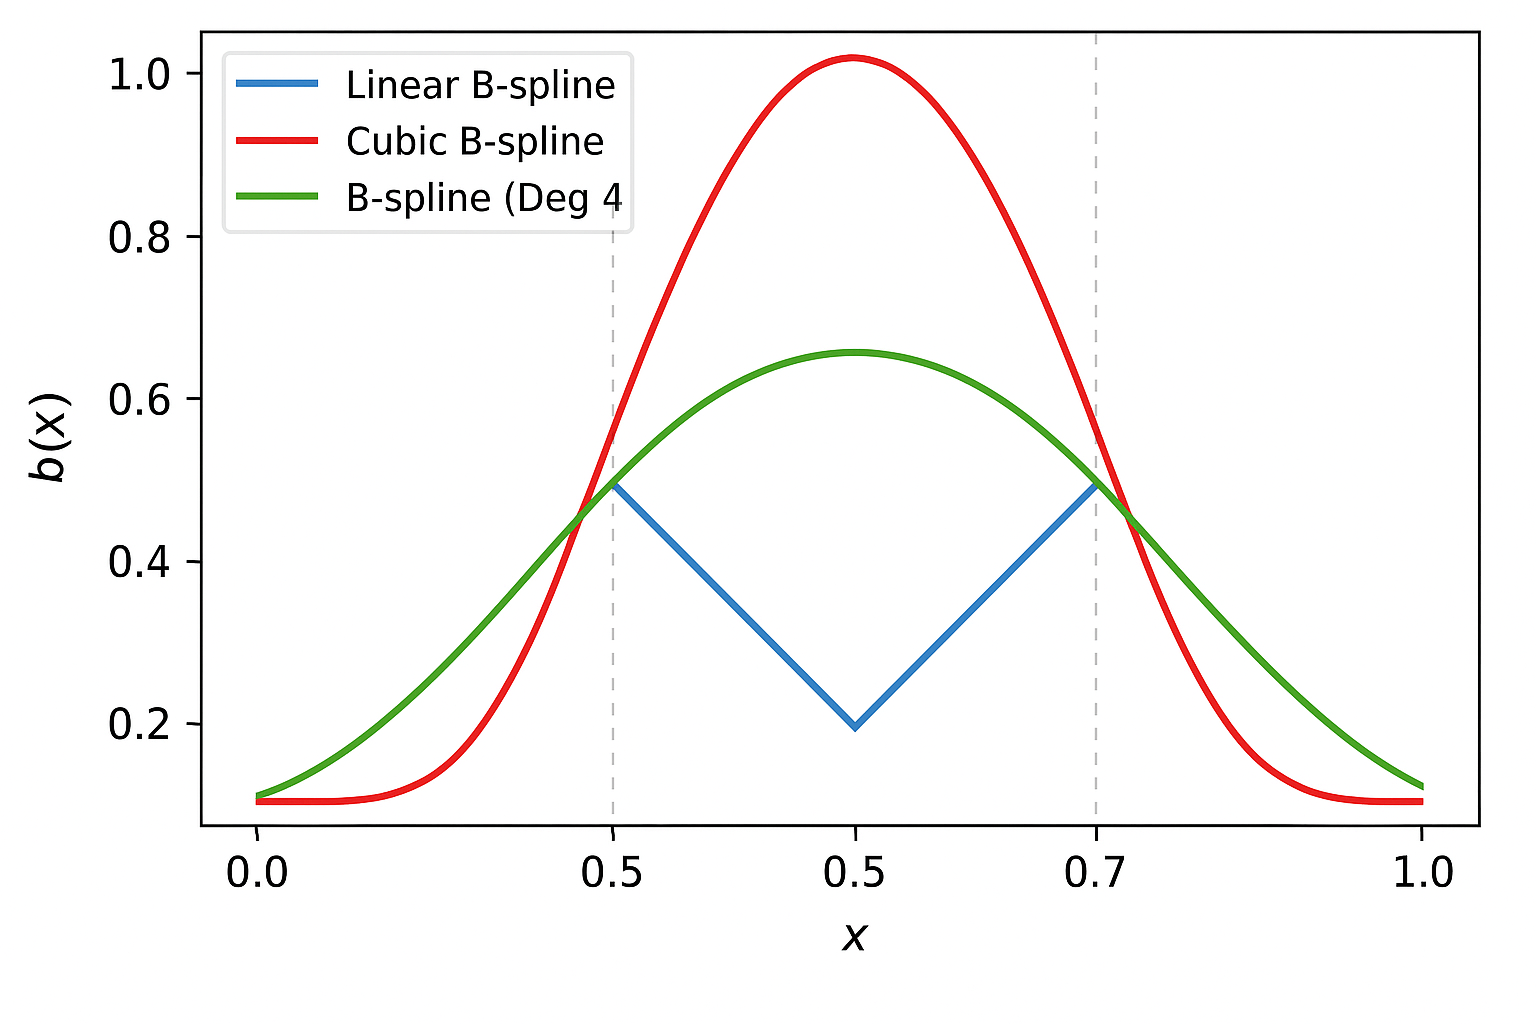
\includegraphics{fig/bsplinescomp.png}

The higher the degree, the smoother the spline:

\begin{itemize}
\tightlist
\item
  Linear → sharp slope changes\\
\item
  Quadratic → gentle curves\\
\item
  Cubic → continuous curvature and smooth transitions
\end{itemize}

\hypertarget{why-b-splines-work-well}{%
\subsubsection*{Why B-splines Work Well}\label{why-b-splines-work-well}}
\addcontentsline{toc}{subsubsection}{Why B-splines Work Well}

Local support keeps each basis function nonzero over only a short
interval, which improves conditioning and computation. Smoothness is
built in: a degree-\(d\) B-spline is continuous with continuous
derivatives up to order \(d-1\) at each knot. Coefficients are not meant
to be interpreted individually; the fitted curve \(\mu(x)\) is the
target.

\begin{tcolorbox}[enhanced jigsaw, breakable, colbacktitle=quarto-callout-note-color!10!white, left=2mm, colframe=quarto-callout-note-color-frame, opacityback=0, coltitle=black, colback=white, rightrule=.15mm, title=\textcolor{quarto-callout-note-color}{\faInfo}\hspace{0.5em}{Note}, titlerule=0mm, opacitybacktitle=0.6, leftrule=.75mm, toprule=.15mm, arc=.35mm, bottomtitle=1mm, toptitle=1mm, bottomrule=.15mm]

\textbf{Rule of thumb.} Use cubic B-splines (degree = 3) for smooth
regression curves. Choose knot number and placement pragmatically (e.g.,
quantiles of \(x\) or evenly spaced over the data range). B-splines also
integrate naturally with penalties and GAMs when you want automatic
smoothness selection.

\end{tcolorbox}

\begin{center}\rule{0.5\linewidth}{0.5pt}\end{center}

\hypertarget{fitting-b-splines-in-r}{%
\subsection*{Fitting B-Splines in R}\label{fitting-b-splines-in-r}}
\addcontentsline{toc}{subsection}{Fitting B-Splines in R}

\begin{Shaded}
\begin{Highlighting}[]
\FunctionTok{library}\NormalTok{(splines)    }

    \CommentTok{\#Linear splines}
\NormalTok{    fit1 }\OtherTok{\textless{}{-}} \FunctionTok{lm}\NormalTok{(bw }\SpecialCharTok{\textasciitilde{}} \FunctionTok{bs}\NormalTok{(gw, }\AttributeTok{knots =} \FunctionTok{c}\NormalTok{(}\DecValTok{37}\NormalTok{, }\DecValTok{42}\NormalTok{), }\AttributeTok{degree=}\DecValTok{1}\NormalTok{), }\AttributeTok{data =}\NormalTok{ dat)}
    \CommentTok{\#Quadratic splines}
\NormalTok{    fit2 }\OtherTok{\textless{}{-}} \FunctionTok{lm}\NormalTok{(bw }\SpecialCharTok{\textasciitilde{}} \FunctionTok{bs}\NormalTok{(gw, }\AttributeTok{knots =} \FunctionTok{c}\NormalTok{(}\DecValTok{37}\NormalTok{, }\DecValTok{42}\NormalTok{), }\AttributeTok{degree=}\DecValTok{2}\NormalTok{), }\AttributeTok{data =}\NormalTok{ dat)}
    \CommentTok{\#Cubic splines}
\NormalTok{    fit3 }\OtherTok{\textless{}{-}} \FunctionTok{lm}\NormalTok{(bw }\SpecialCharTok{\textasciitilde{}} \FunctionTok{bs}\NormalTok{(gw, }\AttributeTok{knots =} \FunctionTok{c}\NormalTok{(}\DecValTok{37}\NormalTok{, }\DecValTok{42}\NormalTok{), }\AttributeTok{degree=}\DecValTok{3}\NormalTok{), }\AttributeTok{data =}\NormalTok{ dat)}
\end{Highlighting}
\end{Shaded}


\includegraphics{Module_4B_Splines_files/figure-pdf/unnamed-chunk-7-1.pdf}

\textbf{Model Interpretation:}

\begin{itemize}
\item
  \textbf{Role of Coefficients}:

  \begin{itemize}
  \item
    In a spline model, the estimated coefficients \(\beta_k\) represent
    the contribution of each B-spline basis function \(b_k(x)\) to the
    overall predicted value of the response variable \(\mu(x)\).
  \item
    Each coefficient \(\beta_k\) adjusts the height and influence of its
    corresponding B-spline function across the range of \(x\).
  \end{itemize}
\item
  \textbf{Effect on the Prediction}:

  \begin{itemize}
  \tightlist
  \item
    The overall model prediction \(\mu(x)\) is a linear combination of
    the B-spline basis functions weighted by their respective
    coefficients. Thus, the predicted value at a given \(x\) is
    influenced by the specific values of these coefficients and the
    corresponding basis functions evaluated at \(x\).
  \end{itemize}
\item
  \textbf{Local Interpretation}:

  \begin{itemize}
  \item
    The interpretation of a specific coefficient \(\beta_k\) is often
    local rather than global:

    \begin{itemize}
    \item
      If \(\beta_k\) is positive, it indicates that the B-spline
      function \(b_k(x)\) contributes positively to the predicted value
      of \(\mu(x)\) in the range where \(b_k(x)\) is non-zero.
    \item
      If \(\beta_k\) is negative, it implies a negative contribution
      from \(b_k(x)\) in its active range.
    \end{itemize}
  \end{itemize}
\item
  \textbf{Influence of Knots}:

  \begin{itemize}
  \item
    The placement of knots influences the shape of the spline and,
    consequently, how the coefficients interact with the data:

    \begin{itemize}
    \tightlist
    \item
      The regions between knots allow for changes in the slope and
      curvature of the spline. Thus, the coefficients can be seen as
      controlling the smooth transitions between these segments.
    \end{itemize}
  \end{itemize}
\end{itemize}

\begin{center}\rule{0.5\linewidth}{0.5pt}\end{center}

\hypertarget{section-26}{%
\subsection*{\texorpdfstring{\textcolor{green}{Data Description: NYC Daily Mortality and Air Pollution Dataset}}{}}\label{section-26}}
\addcontentsline{toc}{subsection}{\textcolor{green}{Data Description: NYC Daily Mortality and Air Pollution Dataset}}

The dataset contains \textbf{daily time-series data from New York City}
and is widely used in environmental epidemiology for demonstrating
regression and smoothing techniques. The data were originally compiled
as part of \textbf{NMMAPS}, a multi-city study assessing the short-term
health effects of air pollution across major U.S. cities. New York City
serves as a canonical example for time-series regression because it
exhibits:

\begin{itemize}
\tightlist
\item
  pronounced \textbf{seasonal and temperature-related mortality
  patterns}, and\\
\item
  measurable day-to-day variation in \textbf{PM₂.₅} (fine particulate
  matter).
\end{itemize}

Each observation represents \textbf{one day} of data for New York City
between \textbf{2001 and 2005}.\\
The dataset includes information on \textbf{daily mortality counts},
\textbf{air-pollution levels}, and \textbf{meteorological variables}
such as temperature and dew-point temperature.

\begin{longtable}[]{@{}
  >{\raggedright\arraybackslash}p{(\columnwidth - 2\tabcolsep) * \real{0.5000}}
  >{\raggedright\arraybackslash}p{(\columnwidth - 2\tabcolsep) * \real{0.5000}}@{}}
\toprule\noalign{}
\begin{minipage}[b]{\linewidth}\raggedright
\textbf{Variable}
\end{minipage} & \begin{minipage}[b]{\linewidth}\raggedright
\textbf{Description}
\end{minipage} \\
\midrule\noalign{}
\endhead
\bottomrule\noalign{}
\endlastfoot
\texttt{date} & Calendar date (YYYY-MM-DD). \\
\texttt{alldeaths} & Total number of all-cause deaths per day in New
York City. \\
\texttt{age65plus} & Number of daily deaths among individuals aged 65
years and older. \\
\texttt{cardioresp} & Daily number of deaths from cardiovascular or
respiratory causes (all ages). \\
\texttt{cr65plus} & Cardiovascular or respiratory deaths among those
aged 65+. \\
\texttt{dow} & Day of the week (Monday -- Sunday). \\
\texttt{pm25} & Daily mean fine particulate-matter concentration
(µg/m³). \\
\texttt{Temp} & Daily mean ambient temperature (°F). \\
\texttt{DpTemp} & Daily mean dew-point temperature (°F). \\
\texttt{rmTemp} & Running mean temperature (typically a 3- or 5-day
moving average). \\
\texttt{rmDpTemp} & Running mean dew-point temperature. \\
\end{longtable}

\begin{Shaded}
\begin{Highlighting}[]
\CommentTok{\# Load data}
\FunctionTok{load}\NormalTok{(}\FunctionTok{file.path}\NormalTok{(}\FunctionTok{getwd}\NormalTok{(), }\StringTok{"data"}\NormalTok{, }\StringTok{"NYC.RData"}\NormalTok{))  }\CommentTok{\# expects object \textasciigrave{}health\textasciigrave{}}

\CommentTok{\# Ensure date is numeric for bs(); keep original for labeling}
\NormalTok{health}\SpecialCharTok{$}\NormalTok{date\_num }\OtherTok{\textless{}{-}} \FunctionTok{as.numeric}\NormalTok{(health}\SpecialCharTok{$}\NormalTok{date)}

\NormalTok{plot\_bs\_panel }\OtherTok{\textless{}{-}} \ControlFlowTok{function}\NormalTok{(df, main\_title) \{}
  \CommentTok{\# Build a common prediction grid (sorted by date)}
\NormalTok{  ord   }\OtherTok{\textless{}{-}} \FunctionTok{order}\NormalTok{(health}\SpecialCharTok{$}\NormalTok{date)}
\NormalTok{  xgrid }\OtherTok{\textless{}{-}} \FunctionTok{data.frame}\NormalTok{(}\AttributeTok{date      =}\NormalTok{ health}\SpecialCharTok{$}\NormalTok{date[ord],}
                      \AttributeTok{date\_num  =}\NormalTok{ health}\SpecialCharTok{$}\NormalTok{date\_num[ord])}

  \CommentTok{\# Fit linear/quadratic/cubic B{-}splines in a compact way}
\NormalTok{  f1 }\OtherTok{\textless{}{-}} \FunctionTok{lm}\NormalTok{(alldeaths }\SpecialCharTok{\textasciitilde{}} \FunctionTok{bs}\NormalTok{(date\_num, }\AttributeTok{df =}\NormalTok{ df, }\AttributeTok{degree =} \DecValTok{1}\NormalTok{), }\AttributeTok{data =}\NormalTok{ health)}
\NormalTok{  f2 }\OtherTok{\textless{}{-}} \FunctionTok{lm}\NormalTok{(alldeaths }\SpecialCharTok{\textasciitilde{}} \FunctionTok{bs}\NormalTok{(date\_num, }\AttributeTok{df =}\NormalTok{ df, }\AttributeTok{degree =} \DecValTok{2}\NormalTok{), }\AttributeTok{data =}\NormalTok{ health)}
\NormalTok{  f3 }\OtherTok{\textless{}{-}} \FunctionTok{lm}\NormalTok{(alldeaths }\SpecialCharTok{\textasciitilde{}} \FunctionTok{bs}\NormalTok{(date\_num, }\AttributeTok{df =}\NormalTok{ df, }\AttributeTok{degree =} \DecValTok{3}\NormalTok{), }\AttributeTok{data =}\NormalTok{ health)}

  \CommentTok{\# Number of interior knots=df−(d+1)}
  
  
  \CommentTok{\# Predicted values on sorted grid}
\NormalTok{  p1 }\OtherTok{\textless{}{-}} \FunctionTok{predict}\NormalTok{(f1, }\AttributeTok{newdata =}\NormalTok{ xgrid)}
\NormalTok{  p2 }\OtherTok{\textless{}{-}} \FunctionTok{predict}\NormalTok{(f2, }\AttributeTok{newdata =}\NormalTok{ xgrid)}
\NormalTok{  p3 }\OtherTok{\textless{}{-}} \FunctionTok{predict}\NormalTok{(f3, }\AttributeTok{newdata =}\NormalTok{ xgrid)}

  \CommentTok{\# Grab interior knots for the linear case (they’re the same knot locations for a given df)}
\NormalTok{  B  }\OtherTok{\textless{}{-}} \FunctionTok{bs}\NormalTok{(health}\SpecialCharTok{$}\NormalTok{date\_num, }\AttributeTok{df =}\NormalTok{ df, }\AttributeTok{degree =} \DecValTok{1}\NormalTok{)}
\NormalTok{  ks }\OtherTok{\textless{}{-}} \FunctionTok{attr}\NormalTok{(B, }\StringTok{"knots"}\NormalTok{)}

  \CommentTok{\# Scatter + fitted lines}
  \FunctionTok{plot}\NormalTok{(health}\SpecialCharTok{$}\NormalTok{alldeaths }\SpecialCharTok{\textasciitilde{}}\NormalTok{ health}\SpecialCharTok{$}\NormalTok{date, }\AttributeTok{col =} \StringTok{"grey60"}\NormalTok{, }\AttributeTok{pch =} \DecValTok{16}\NormalTok{, }\AttributeTok{cex =} \FloatTok{0.6}\NormalTok{,}
       \AttributeTok{xlab =} \StringTok{"Date"}\NormalTok{, }\AttributeTok{ylab =} \StringTok{"Daily deaths"}\NormalTok{, }\AttributeTok{main =}\NormalTok{ main\_title)}
  \FunctionTok{lines}\NormalTok{(xgrid}\SpecialCharTok{$}\NormalTok{date\_num, p1, }\AttributeTok{col =} \DecValTok{2}\NormalTok{, }\AttributeTok{lwd =} \DecValTok{3}\NormalTok{)}
  \FunctionTok{lines}\NormalTok{(xgrid}\SpecialCharTok{$}\NormalTok{date\_num, p2, }\AttributeTok{col =} \DecValTok{4}\NormalTok{, }\AttributeTok{lwd =} \DecValTok{3}\NormalTok{)}
  \FunctionTok{lines}\NormalTok{(xgrid}\SpecialCharTok{$}\NormalTok{date\_num, p3, }\AttributeTok{col =} \DecValTok{5}\NormalTok{, }\AttributeTok{lwd =} \DecValTok{3}\NormalTok{)}

  \CommentTok{\# Show interior knots}
  \ControlFlowTok{if}\NormalTok{ (}\SpecialCharTok{!}\FunctionTok{is.null}\NormalTok{(ks) }\SpecialCharTok{\&\&} \FunctionTok{length}\NormalTok{(ks) }\SpecialCharTok{\textgreater{}} \DecValTok{0}\NormalTok{) }\FunctionTok{abline}\NormalTok{(}\AttributeTok{v =} \FunctionTok{as.Date}\NormalTok{(ks, }\AttributeTok{origin =} \StringTok{"1970{-}01{-}01"}\NormalTok{),}
                                             \AttributeTok{col =} \StringTok{"grey80"}\NormalTok{, }\AttributeTok{lty =} \DecValTok{2}\NormalTok{)}

  \FunctionTok{legend}\NormalTok{(}\StringTok{"topleft"}\NormalTok{,}
         \AttributeTok{legend =} \FunctionTok{c}\NormalTok{(}\StringTok{"Linear (deg=1)"}\NormalTok{, }\StringTok{"Quadratic (deg=2)"}\NormalTok{, }\StringTok{"Cubic (deg=3)"}\NormalTok{),}
         \AttributeTok{col =} \FunctionTok{c}\NormalTok{(}\DecValTok{2}\NormalTok{, }\DecValTok{4}\NormalTok{, }\DecValTok{5}\NormalTok{), }\AttributeTok{lwd =} \DecValTok{3}\NormalTok{, }\AttributeTok{bty =} \StringTok{"n"}\NormalTok{, }\AttributeTok{cex =} \FloatTok{1.0}\NormalTok{)}
\NormalTok{\}}

\CommentTok{\# Two{-}panel comparison: df = 10 vs df = 20}
\NormalTok{op }\OtherTok{\textless{}{-}} \FunctionTok{par}\NormalTok{(}\AttributeTok{mfrow =} \FunctionTok{c}\NormalTok{(}\DecValTok{1}\NormalTok{, }\DecValTok{2}\NormalTok{), }\AttributeTok{mar =} \FunctionTok{c}\NormalTok{(}\DecValTok{4}\NormalTok{, }\DecValTok{4}\NormalTok{, }\DecValTok{4}\NormalTok{, }\DecValTok{1}\NormalTok{))}
\FunctionTok{plot\_bs\_panel}\NormalTok{(}\AttributeTok{df =} \DecValTok{10}\NormalTok{, }\AttributeTok{main\_title =} \StringTok{"B{-}splines on Date (df = 10)"}\NormalTok{)}
\FunctionTok{plot\_bs\_panel}\NormalTok{(}\AttributeTok{df =} \DecValTok{20}\NormalTok{, }\AttributeTok{main\_title =} \StringTok{"B{-}splines on Date (df = 20)"}\NormalTok{)}
\end{Highlighting}
\end{Shaded}

\begin{figure}[H]

{\centering 
\includegraphics{Module_4B_Splines_files/figure-pdf/unnamed-chunk-8-1.pdf}

}

\end{figure}

\begin{Shaded}
\begin{Highlighting}[]
\FunctionTok{par}\NormalTok{(op)}
\end{Highlighting}
\end{Shaded}

\hypertarget{choices-we-have-to-make}{%
\subsubsection*{Choices we have to
make:}\label{choices-we-have-to-make}}
\addcontentsline{toc}{subsubsection}{Choices we have to make:}

\begin{itemize}
\item
  We need to pick:

  \begin{itemize}
  \item
    Which basis function? Linear versus Cubic
  \item
    How many knots?
  \item
    Where to put the knots?
  \end{itemize}
\item
  Choice of basis function usually does not have a large impact on model
  fit, especially when there are enough knots and \(g(x)\) is smooth.
\item
  When there are enough knots, their locations are less important too!
  By ``enough'' this means distance between them is small enough to
  capture fluctuations.
\item
  So \textbf{how many knots?} is the question.
\end{itemize}

\begin{tcolorbox}[enhanced jigsaw, breakable, colbacktitle=quarto-callout-important-color!10!white, left=2mm, colframe=quarto-callout-important-color-frame, opacityback=0, coltitle=black, colback=white, rightrule=.15mm, title=\textcolor{quarto-callout-important-color}{\faExclamation}\hspace{0.5em}{Important}, titlerule=0mm, opacitybacktitle=0.6, leftrule=.75mm, toprule=.15mm, arc=.35mm, bottomtitle=1mm, toptitle=1mm, bottomrule=.15mm]

\textbf{\emph{Bias- Variance Tradeoff}}

\begin{itemize}
\item
  More knots-\textgreater{}

  \begin{itemize}
  \item
    can better capture fine scale trends
  \item
    Need to estimate more coefficients (risk of overfitting)
  \item
    Below shows cubic splines with different number of knots.
  \end{itemize}
\end{itemize}


\includegraphics{Module_4B_Splines_files/figure-pdf/unnamed-chunk-9-1.pdf}

\end{tcolorbox}

\begin{center}\rule{0.5\linewidth}{0.5pt}\end{center}

\hypertarget{section-27}{%
\subsection*{\texorpdfstring{\textcolor{green}{Model Assessment: Bias–Variance and Cross-Validation}}{}}\label{section-27}}
\addcontentsline{toc}{subsection}{\textcolor{green}{Model Assessment: Bias–Variance and Cross-Validation}}

Assume the data come from some \emph{true} underlying model:

\[
Y = g(X) + \varepsilon, \quad \varepsilon \sim N(0, \sigma^2)
\]

Here:

\begin{itemize}
\tightlist
\item
  \(g(X)\) is the \emph{true, unknown regression function}, and\\
\item
  \(\varepsilon\) is random noise, independent of \(X\).
\end{itemize}

Our goal is to estimate \(g(X)\) with a model \(\hat{g}(X)\) that
predicts new observations accurately.

For a given \(x_i\):

\[
\hat{Y}_i = \hat{g}(x_i)
\]

and we assume \(g(x_i) \perp \varepsilon_i\) (the model and noise are
independent). We use several metrics to assess model fit:

\textbf{1. Population Mean Squared Error (MSE):} The \textbf{expected
squared difference} between the true \(Y\) and its estimate
\(\hat{g}(x)\) defines the \emph{population Mean Squared Error} (MSE):

\[
\text{MSE} = E[(Y - \hat{g}(X))^2]
\]

Expanding this expectation gives the classic \textbf{bias--variance
decomposition}:

\[
E[(Y - \hat{g}(X))^2] =
\underbrace{\sigma^2}_{\text{Irreducible error}}
+ \underbrace{[E(\hat{g}(X)) - g(X)]^2}_{\text{Bias}^2}
+ \underbrace{E[(\hat{g}(X) - E[\hat{g}(X)])^2]}_{\text{Variance}}
\]

\begin{itemize}
\tightlist
\item
  \textbf{Bias} measures how far the \emph{average fitted curve} is from
  the true function \(g(x)\).\\
\item
  \textbf{Variance} measures how much the fitted function \(\hat{g}(x)\)
  fluctuates across samples.\\
\item
  The \textbf{irreducible error} \(\sigma^2\) cannot be reduced no
  matter how good our model is.
\end{itemize}

Our goal is to choose a model that \textbf{minimizes the MSE}, balancing
\textbf{bias and variance}.

\textbf{2. Estimating Prediction Error: Cross-Validation:} In practice,
the true \(g(x)\) and \(\sigma^2\) are unknown, so we approximate MSE
using \textbf{cross-validation}.

Let \(\hat{g}^{(-i)}(x_i)\) denote the predicted value for \(y_i\)
obtained by fitting the model on all observations \emph{except} the
\(i^{th}\) one.\\
Then the \textbf{Leave-One-Out Cross-Validation (LOOCV)} statistic is:

\[
CV = \frac{1}{n} \sum_{i=1}^{n} \big(y_i - \hat{g}^{(-i)}(x_i)\big)^2
\]

This provides an \textbf{approximately unbiased estimate of the
population MSE}:

\[
CV \approx E[(Y - \hat{g}(X))^2]
\]

\textbf{Interpretation:}

\begin{itemize}
\tightlist
\item
  Cross-validation mimics how well our model predicts \emph{new} unseen
  data.\\
\item
  A model with low CV error generalizes well beyond the training
  sample.\\
\item
  \textbf{We choose the model (or smoothing level) that minimizes CV.}
\end{itemize}

\hypertarget{overfitting-and-underfitting}{%
\subsubsection*{Overfitting and
Underfitting}\label{overfitting-and-underfitting}}
\addcontentsline{toc}{subsubsection}{Overfitting and Underfitting}

The \textbf{bias--variance tradeoff} determines whether a model overfits
or underfits the data.

\begin{longtable}[]{@{}
  >{\raggedright\arraybackslash}p{(\columnwidth - 8\tabcolsep) * \real{0.2000}}
  >{\raggedright\arraybackslash}p{(\columnwidth - 8\tabcolsep) * \real{0.2000}}
  >{\centering\arraybackslash}p{(\columnwidth - 8\tabcolsep) * \real{0.2000}}
  >{\centering\arraybackslash}p{(\columnwidth - 8\tabcolsep) * \real{0.2000}}
  >{\raggedright\arraybackslash}p{(\columnwidth - 8\tabcolsep) * \real{0.2000}}@{}}
\toprule\noalign{}
\begin{minipage}[b]{\linewidth}\raggedright
\textbf{Model Behavior}
\end{minipage} & \begin{minipage}[b]{\linewidth}\raggedright
\textbf{Description}
\end{minipage} & \begin{minipage}[b]{\linewidth}\centering
\textbf{Bias}
\end{minipage} & \begin{minipage}[b]{\linewidth}\centering
\textbf{Variance}
\end{minipage} & \begin{minipage}[b]{\linewidth}\raggedright
\textbf{Example (Splines)}
\end{minipage} \\
\midrule\noalign{}
\endhead
\bottomrule\noalign{}
\endlastfoot
\textbf{Overfitting} & Model captures noise rather than the true signal
(\(\hat{g}(x_i) \approx g(x_i) + \varepsilon_i\)). & Low & High & Very
wiggly spline; too many knots or high \texttt{df}. \\
\textbf{Underfitting} & Model too simple to capture the structure
(\(\hat{g}(x_i)\) is overly smooth). & High & Low & Almost flat spline;
too few knots or low \texttt{df}. \\
\end{longtable}

From the \textbf{spline perspective}:

\begin{itemize}
\tightlist
\item
  Very \textbf{wiggly} splines → \textbf{high variance}, low bias.\\
\item
  Very \textbf{smooth} splines → \textbf{high bias}, low variance.
\end{itemize}

We aim for the \textbf{sweet spot}: smooth enough to generalize,
flexible enough to fit structure.

\textbf{From Hastie, Tibshirani \& Friedman (2009):}\\
``Discussions of error rate estimation can be confusing because we must
be clear which quantities are fixed and which are random.''\\
CV keeps \(x_i\) fixed and estimates prediction error over different
possible samples of \(\varepsilon_i\).

\begin{center}\rule{0.5\linewidth}{0.5pt}\end{center}

\hypertarget{section-28}{%
\section*{\texorpdfstring{\textcolor{purple}{Summary}}{}}\label{section-28}}
\addcontentsline{toc}{section}{\textcolor{purple}{Summary}}

\markright{\textcolor{purple}{Summary}}

\begin{longtable}[]{@{}
  >{\raggedright\arraybackslash}p{(\columnwidth - 2\tabcolsep) * \real{0.5000}}
  >{\raggedright\arraybackslash}p{(\columnwidth - 2\tabcolsep) * \real{0.5000}}@{}}
\toprule\noalign{}
\begin{minipage}[b]{\linewidth}\raggedright
\textbf{Section}
\end{minipage} & \begin{minipage}[b]{\linewidth}\raggedright
\textbf{Description}
\end{minipage} \\
\midrule\noalign{}
\endhead
\bottomrule\noalign{}
\endlastfoot
\textbf{Model Setup} & Unknown regression function modeled via
\textbf{basis expansion}:
\(y_i = g(x_i) + \varepsilon_i,\ \varepsilon_i\sim N(0,\sigma^2)\)
\(g(x_i) = \sum_{m=1}^M \beta_m\, b_m(x_i)\). \\
\textbf{Truncated Power (Parametric) Splines} & Polynomial plus
\textbf{knoted adjustments} using truncated terms:
\(y_i = \beta_0 + \sum_{j=1}^d \beta_j x_i^j + \sum_{m=1}^M \gamma_m (x_i-k_m)_+^{\,d}\),
where \((x-\kappa)_+^{\,d} = (x-\kappa)^d\mathbf{1}\{x>\kappa\}\).
Flexible, but can be \textbf{numerically unstable} with many knots/high
degree. \\
\textbf{Continuity by Degree} & \textbf{Linear (}\(d=1\)): \(C^0\)
(function continuous; slope can jump). \textbf{Quadratic (}\(d=2\)):
\(C^1\) (continuous slope). \textbf{Cubic (}\(d=3\)): \(C^2\)
(continuous curvature) --- typically preferred. \\
\textbf{Linear Spline (worked form)} & With knots \(36.5, 41.5\):
\(y_i=\beta_0+\beta_1 x_i+\beta_2(x_i-36.5)_+ + \beta_3(x_i-41.5)_+ + \varepsilon_i\).
Slope changes are \(\beta_2,\beta_3\); segments share continuity at
knots. \\
\textbf{Cubic Spline (worked form)} & With knots \(\kappa_1,\kappa_2\):
\(g(x_i)=\beta_0+\beta_1x_i+\beta_2x_i^2+\beta_3x_i^3+\beta_4(x_i-\kappa_1)_+^{\,3}+\beta_5(x_i-\kappa_2)_+^{\,3}\).
Ensures continuity of function, slope, and curvature. \\
\textbf{B-Splines (Basis Splines)} & Reparameterize the same spline
space into \textbf{localized, well-conditioned} basis functions (smooth
``bumps'' with \textbf{local support}). Model:
\(\mu(x_i)=\sum_{k=1}^K \beta_k\, b_k^{(d)}(x_i)\), with design matrix
\(B_{ik}=b_k^{(d)}(x_i)\). \textbf{Cox--de Boor recursion} builds
\(b_k^{(d)}\) from \(b_k^{(d-1)}\); zero-denominator terms treated as
0. \\
\textbf{Why B-Splines?} & Better \textbf{numerical stability},
\textbf{sparser} design (local support), easy to increase flexibility,
and natural for penalties/GAMs. Coefficients are \textbf{not} directly
interpretable; focus on the \textbf{fitted curve}. \\
\textbf{Degrees of Freedom \& Knots} & In \texttt{splines::bs()},
\textbf{df = number of basis columns} (no intercept). For degree \(d\):
\textbf{Interior knots} \(=\) \(\text{df}-(d+1)\). More df ⇒ more
flexibility (risk of variance/overfit). \\
\textbf{Choosing Knots} & Start with \textbf{quantiles} or \textbf{even
spacing} over \(x\). With \textbf{enough knots}, exact locations matter
less than the \textbf{number} of knots for smooth \(g(x)\). \\
\textbf{R Quick Reference} & \textbf{Fixed knots:}
\texttt{bs(x,\ knots\ =\ c(...),\ degree\ =\ 1/2/3)} \textbf{By df:}
\texttt{bs(x,\ df\ =\ 10,\ degree\ =\ 3)} \textbf{Extract knots:}
\texttt{attr(bs\_obj,\ "knots")} \textbf{Cubic (common):}
\texttt{degree\ =\ 3} \textbf{Date x:} convert to numeric first. \\
\textbf{Interpretation (Local)} & Each \(\beta_k\) primarily affects
\(\mu(x)\) where \(b_k^{(d)}(x)\) is nonzero (near its knot span).
Changes in knots/df change \textbf{where/how} the curve can flex. \\
\textbf{Model Assessment} & \textbf{MSE decomposition:}
\(E[(Y-\hat g(X))^2]=\sigma^2+\text{Bias}^2+\text{Var}\). \textbf{CV
(LOOCV):} \(\text{CV}=\frac{1}{n}\sum_{i}(y_i-\hat g^{(-i)}(x_i))^2\) ≈
test error. Pick df/knots to \textbf{minimize CV}, balancing
bias--variance. \\
\end{longtable}

\bookmarksetup{startatroot}

\hypertarget{module-4c-penalized-splines}{%
\chapter*{Module 4C Penalized
Splines}\label{module-4c-penalized-splines}}
\addcontentsline{toc}{chapter}{Module 4C Penalized Splines}

\markboth{Module 4C Penalized Splines}{Module 4C Penalized Splines}

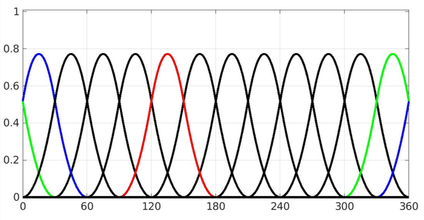
\includegraphics{fig/bsplines.png}

\hypertarget{motivation-and-connection-to-4b}{%
\subsection*{Motivation and Connection to
4B}\label{motivation-and-connection-to-4b}}
\addcontentsline{toc}{subsection}{Motivation and Connection to 4B}

\begin{tcolorbox}[enhanced jigsaw, breakable, colbacktitle=quarto-callout-important-color!10!white, left=2mm, colframe=quarto-callout-important-color-frame, opacityback=0, coltitle=black, colback=white, rightrule=.15mm, title=\textcolor{quarto-callout-important-color}{\faExclamation}\hspace{0.5em}{Motivation}, titlerule=0mm, opacitybacktitle=0.6, leftrule=.75mm, toprule=.15mm, arc=.35mm, bottomtitle=1mm, toptitle=1mm, bottomrule=.15mm]

In Module 4B, we learned about parametric splines, where we fit
piecewise polynomial segments joined at knots. These splines required us
to choose both the number and location of the knots.

If we choose too few knots, the fit is too rigid and misses local
patterns (high bias). If we choose too many knots, the spline can
overfit and capture random noise (high variance).

Question: Is there a way to include many knots for flexibility but
automatically control how wiggly the curve becomes?

Answer: Yes --- by adding a penalty for roughness. This leads to
penalized splines and smoothing splines.

\end{tcolorbox}

\begin{center}\rule{0.5\linewidth}{0.5pt}\end{center}

\hypertarget{penalized-regression-framework-the-idea-behind-penalized-splines}{%
\section*{Penalized Regression Framework: The Idea Behind Penalized
Splines}\label{penalized-regression-framework-the-idea-behind-penalized-splines}}
\addcontentsline{toc}{section}{Penalized Regression Framework: The Idea
Behind Penalized Splines}

\markright{Penalized Regression Framework: The Idea Behind Penalized
Splines}

We begin with the regression model:

\[
y_i = g(x_i) + \varepsilon_i, \quad \varepsilon_i \sim N(0,\sigma^2)
\]

and approximate the unknown function \(g(x)\) using a flexible basis
representation with large fixed \(K\) is \textcolor{red}{unknown}.

Instead of forcing \(g(x)\) to have a specific parametric form, we
approximate it using many basis functions:

\[
g(x) = \sum_{k=1}^K \beta_k b_k(x)
\] In Module 4B, we chose \(K\) by deciding where to put knots. Here we
take a different approach.

The main idea is we start with a lot of knots. This ensures we will not
miss important fine-scale behavior. Next, we assume most of the knots
are not useful and \textcolor{red}{shrink} their coefficients towards
zero. We determine the amount of \textcolor{red}{shrinkage} based on
some criteria (.e.g, CV, GCV, AIC). Benefits of this approach:

\begin{itemize}
\tightlist
\item
  Knot placement is not important if the number if dense enough, but be
  cautious for overfitting.
\item
  Shrinking most coefficients to zero will stabilize model estimation
  similar to performing variable selection.
\item
  Data decide how much flexibility is needed.
\end{itemize}

\begin{center}\rule{0.5\linewidth}{0.5pt}\end{center}

\hypertarget{penalized-least-squares-pls}{%
\section*{Penalized Least Squares
(PLS)}\label{penalized-least-squares-pls}}
\addcontentsline{toc}{section}{Penalized Least Squares (PLS)}

\markright{Penalized Least Squares (PLS)}

\emph{Intuition: Ordinary least squares minimizes the sum of squared
residuals. Penalized least squares adds a second term that discourages
unnecessary complexity in the fitted function.}

To estimate \(g(x)\) we minimize a
\textcolor{blue}{penalized residual sum of squares}:

\[
\text{PLS}(\lambda) = \sum_{i=1}^{n} (y_i - g(x_i))^2 + \underset{\text{roughness}}{\lambda J(g)},
\]

where:

\begin{itemize}
\tightlist
\item
  The first term measures fit to the data.
\item
  The second term \(J(g)\) measures the roughness of the function.
\item
  \(\lambda\) controls the tradeoff between fit and smoothness.
\end{itemize}

\begin{tcolorbox}[enhanced jigsaw, breakable, colbacktitle=quarto-callout-note-color!10!white, left=2mm, colframe=quarto-callout-note-color-frame, opacityback=0, coltitle=black, colback=white, rightrule=.15mm, title=\textcolor{quarto-callout-note-color}{\faInfo}\hspace{0.5em}{Note}, titlerule=0mm, opacitybacktitle=0.6, leftrule=.75mm, toprule=.15mm, arc=.35mm, bottomtitle=1mm, toptitle=1mm, bottomrule=.15mm]

Interpretation of \(\lambda\):

Small \(\lambda\) → minimal penalty → curve follows data closely (wiggly
fit).

Large \(\lambda\) → heavy penalty → smoother curve (may miss fine
details).

\end{tcolorbox}

\begin{center}\rule{0.5\linewidth}{0.5pt}\end{center}

\hypertarget{constrained-vs.-penalized-form}{%
\section*{Constrained vs.~Penalized
Form}\label{constrained-vs.-penalized-form}}
\addcontentsline{toc}{section}{Constrained vs.~Penalized Form}

\markright{Constrained vs.~Penalized Form}

There are two equivalent ways to control how smooth the estimated
function is: we can either place a hard limit on its wiggliness
(constrained form) or penalize wiggliness directly in the objective
function (penalty form).

\begin{itemize}
\tightlist
\item
  (a) Constrained Form:\\
  Minimize \(\sum (y_i - g(x_i))^2\) subject to \(J(g) \leq c\).
\end{itemize}

Here we allow the curve to fit the data but restrict its total
roughness, i.e., fit the data well, but don't let the function be too
rough. The constant \(c\) sets an upperbound on how wiggly \(g(x)\) can
be. This is computationally inconvenient.

Equivalently,

\begin{itemize}
\tightlist
\item
  (b) Penalty Form:\\
  Minimize \(\sum (y_i - g(x_i))^2 + \lambda J(g)\).
\end{itemize}

Here, we trade off between fit and smoothness. The constant \(\lambda\)
acts as a Lagrange multiplier linked to constraint \(c\), i.e., fit the
data and smoothness simultaneously-balancing them through \(\lambda\).

\begin{center}\rule{0.5\linewidth}{0.5pt}\end{center}

\hypertarget{examples-of-pls-using-different-penalties}{%
\section*{Examples of PLS Using Different
Penalties}\label{examples-of-pls-using-different-penalties}}
\addcontentsline{toc}{section}{Examples of PLS Using Different
Penalties}

\markright{Examples of PLS Using Different Penalties}

Penalized Least Squares (PLS) can take different forms depending on what
we choose to penalize

\begin{enumerate}
\def\labelenumi{\Roman{enumi}.}
\tightlist
\item
  \textcolor{red}{Ridge regression}- \(J(g)\) penalizes the \textbf{size
  of the coefficients}.
\end{enumerate}

\[
J(g) = \sum_{m=1}^M \beta_m^2 = ||\beta||_2^2 \leq C
\]

where \(||\beta||_2\) is the L2-Norm and \(C\) is a positive constant.
Ridge regression using the \(L2-\) penalty which does not induce
sparsity because is does not set \(\beta's\) exactly to 0.

\begin{tcolorbox}[enhanced jigsaw, rightrule=.15mm, breakable, left=2mm, colframe=quarto-callout-tip-color-frame, opacityback=0, leftrule=.75mm, toprule=.15mm, colback=white, arc=.35mm, bottomrule=.15mm]

\textbf{L2 Definition}\vspace{2mm}

The L2 norm, also called the Euclidean norm, is a measure of the
magnitude (or length) of a vector in Euclidean space. It is defined as:

\[
\|\mathbf{v}\|_2 = \sqrt{v_1^2 + v_2^2 + \dots + v_n^2} = \sqrt{\sum_{i=1}^n v_i^2}
\]

where \(\mathbf{v} = [v_1, v_2, \dots, v_n]\) is a vector in
\(\mathbb{R}^n\).

The L2 norm is the square root of the sum of the squared elements of the
vector.

Properties:

1. Non-Negativity

\[
\|\mathbf{v}\|_2 \geq 0
\]

\begin{itemize}
\tightlist
\item
  \(\|\mathbf{v}\|_2 = 0\) if and only if \(\mathbf{v} = 0\).
\end{itemize}

\begin{enumerate}
\def\labelenumi{\arabic{enumi}.}
\setcounter{enumi}{1}
\tightlist
\item
  Scalability: If \(c\) is a scalar:
\end{enumerate}

\[
\|c \mathbf{v}\|_2 = |c| \cdot \|\mathbf{v}\|_2
\]

\begin{enumerate}
\def\labelenumi{\arabic{enumi}.}
\setcounter{enumi}{2}
\tightlist
\item
  Triangle Inequality: For two vectors \(\mathbf{u}\) and
  \(\mathbf{v}\):
\end{enumerate}

\[
\|\mathbf{u} + \mathbf{v}\|_2 \leq \|\mathbf{u}\|_2 + \|\mathbf{v}\|_2
\]

\begin{enumerate}
\def\labelenumi{\arabic{enumi}.}
\setcounter{enumi}{3}
\tightlist
\item
  Geometric Interpretation: The L2 norm corresponds to the Euclidean
  distance from the origin to the point \(\mathbf{v}\) in
  \(n\)-dimensional space. For a 2D vector \(\mathbf{v} = [x, y]\), the
  L2 norm is:
\end{enumerate}

\[
\|\mathbf{v}\|_2 = \sqrt{x^2 + y^2}
\]

This is the standard distance formula in 2D geometry.

\end{tcolorbox}

\begin{enumerate}
\def\labelenumi{\Roman{enumi}.}
\setcounter{enumi}{1}
\tightlist
\item
  \textcolor{red}{Lasso}- \(J(g)\) penalizes the \textbf{size of the
  coefficients} using the \(L_1\) norm.
\end{enumerate}

\[
J(g) = \|\beta\|_1 \leq C,
\]\\
where \(\|\beta\|_1\) is the L1-Norm and \(C\) is a positive constant.

LASSO applies an \(L1\) penalty, which encourages sparsity in the
coefficients.\\
Unlike Ridge regression, Lasso can set some \(\beta\)'s exactly to 0,
effectively performing variable selection while also regularizing the
model.

Mathematically, this corresponds to solving:

\[
\min_{\boldsymbol{\beta}} \sum_{i=1}^{n} (y_i - g(x_i))^2 + \lambda \sum_{m=1}^{M} |\beta_m|,
\]

where \(\lambda\) controls the amount of shrinkage.

\begin{tcolorbox}[enhanced jigsaw, rightrule=.15mm, breakable, left=2mm, colframe=quarto-callout-tip-color-frame, opacityback=0, leftrule=.75mm, toprule=.15mm, colback=white, arc=.35mm, bottomrule=.15mm]

\textbf{L1 Definition}\vspace{2mm}

The L1 norm, also known as the Manhattan norm or taxicab norm, measures
the total absolute magnitude of a vector. It is defined as:

\[
\|\mathbf{v}\|_1 = |v_1| + |v_2| + \dots + |v_n| = \sum_{i=1}^n |v_i|
\]

for a vector \(\mathbf{v} = [v_1, v_2, \dots, v_n]\) in
\(\mathbb{R}^n\).

Properties:

\begin{enumerate}
\def\labelenumi{\arabic{enumi}.}
\item
  Non-Negativity:\\
  \[
  \|\mathbf{v}\|_1 \geq 0, \quad \text{and } \|\mathbf{v}\|_1 = 0 \text{ iff } \mathbf{v} = 0.
  \]
\item
  Scalability: For a scalar \(c\):\\
  \[
  \|c\mathbf{v}\|_1 = |c| \cdot \|\mathbf{v}\|_1
  \]
\item
  Triangle Inequality: For any vectors \(\mathbf{u}\) and
  \(\mathbf{v}\):\\
  \[
  \|\mathbf{u} + \mathbf{v}\|_1 \leq \|\mathbf{u}\|_1 + \|\mathbf{v}\|_1
  \]
\item
  Geometric Interpretation:\\
  The L1 norm corresponds to the sum of absolute distances along each
  axis from the origin to the point \(\mathbf{v}\).\\
  In 2D, this is the total ``city-block distance'' you'd travel along
  grid lines:\\
  \[
  \|\mathbf{v}\|_1 = |x| + |y|
  \]\\
  The L1 constraint region forms a diamond shape in 2D, which causes
  some coefficients to hit exactly zero---unlike the circular constraint
  region in Ridge regression.\\
\end{enumerate}

\end{tcolorbox}

\textcolor{blue}{Connection to Penalized Splines:} Ridge and Lasso are
both examples of the penalized least squares framework:

\[
\sum_i (y_i - g(x_i))^2 + \lambda J(g)
\] In these cases, \(J(g)\) penalizes the \ul{size of the coefficients}.

\begin{center}\rule{0.5\linewidth}{0.5pt}\end{center}

\hypertarget{pls-moving-from-constraints-to-penalties}{%
\section*{PLS: Moving from Constraints to
Penalties}\label{pls-moving-from-constraints-to-penalties}}
\addcontentsline{toc}{section}{PLS: Moving from Constraints to
Penalties}

\markright{PLS: Moving from Constraints to Penalties}

For \textcolor{red}{Penalized Spline}, the same principle is used ---
but \(J(g)\) penalizes the \emph{roughness of the function, rather than
the size of the coefficients.} In other words, the penalty smooths the
\textbf{entire fitted curve}, not just the individual coefficients.

Mathematically, this is achieved y penalizing the integrated squared
second derivative:\\
\[
J(g) = \int [g''(x)]^2 dx
\]

This quantity measures how rapidly the function \(g(x)\) bends or
changes curvature (wiggliness). Large values of \(J(g)\) indicate a very
wiggly function, while smaller values correspond to smoother curves.\\
By adding \(\lambda J(g)\) to our objective function, we control the
trade-off between smoothness and fit.

\begin{center}\rule{0.5\linewidth}{0.5pt}\end{center}

\hypertarget{deriving-the-penalized-spline-solution}{%
\subsection*{Deriving the Penalized Spline
Solution}\label{deriving-the-penalized-spline-solution}}
\addcontentsline{toc}{subsection}{Deriving the Penalized Spline
Solution}

We now express the penalized spline problem in matrix form. This will
show that the solution has the same algebraic form as ridge regression,
even though the penalty targets curvature rather than coefficient size.

Let \(\mathbf{B}\) be the basis matrix (each column a basis function
evaluated at all \(x_i\)), and let \(\boldsymbol{\beta}\) be the
corresponding coefficient vector. Then the PLS criterion can be written
as

\[
\text{PLS}(\lambda) = (\mathbf{y} - \mathbf{B}\boldsymbol{\beta})'(\mathbf{y} - \mathbf{B}\boldsymbol{\beta}) + \lambda \underbrace{\boldsymbol{\beta}'\mathbf{K}\boldsymbol{\beta}}_{J(g) = \int[g''(x)]^2dx},
\]

where \(\mathbf{K}\) is a known penalty matrix that encodes curvature or
``wiggliness'' of the fitted function.Typically, \(\mathbf{K}\) is
derived from \(\int b_k''(x)b_l''(x)dx\), so that large curvature is
penalized.

\hypertarget{derivation-of-the-closed-form-solution}{%
\subsection*{\texorpdfstring{\ul{Derivation of the Closed-Form
Solution}}{Derivation of the Closed-Form Solution}}\label{derivation-of-the-closed-form-solution}}
\addcontentsline{toc}{subsection}{\ul{Derivation of the Closed-Form
Solution}}

\hypertarget{optimization-problem}{%
\subsubsection*{\texorpdfstring{\emph{Optimization
Problem}}{Optimization Problem}}\label{optimization-problem}}
\addcontentsline{toc}{subsubsection}{\emph{Optimization Problem}}

We seek to minimize the penalized least squares criterion:

\[
\underset{\boldsymbol{\beta}}{\text{minimize}} 
\quad (\mathbf{y} - \mathbf{B}\boldsymbol{\beta})'(\mathbf{y} - \mathbf{B}\boldsymbol{\beta})
+ \lambda\, \boldsymbol{\beta}'\mathbf{K}\boldsymbol{\beta}.
\]

\hypertarget{differentiate-with-respect-to-boldsymbolbeta}{%
\subsubsection*{\texorpdfstring{1. Differentiate with respect to
\(\boldsymbol{\beta}\)}{1. Differentiate with respect to \textbackslash boldsymbol\{\textbackslash beta\}}}\label{differentiate-with-respect-to-boldsymbolbeta}}
\addcontentsline{toc}{subsubsection}{1. Differentiate with respect to
\(\boldsymbol{\beta}\)}

\[
-2\mathbf{B}'(\mathbf{y} - \mathbf{B}\boldsymbol{\beta}) + 2\lambda\mathbf{K}\boldsymbol{\beta} = 0.
\]

\hypertarget{simplify}{%
\subsubsection*{2. Simplify}\label{simplify}}
\addcontentsline{toc}{subsubsection}{2. Simplify}

\[
\mathbf{B}'\mathbf{B}\boldsymbol{\beta} + \lambda\mathbf{K}\boldsymbol{\beta} = \mathbf{B}'\mathbf{y}.
\]

\hypertarget{rearrange-terms}{%
\subsubsection*{3. Rearrange Terms}\label{rearrange-terms}}
\addcontentsline{toc}{subsubsection}{3. Rearrange Terms}

\[
(\mathbf{B}'\mathbf{B} + \lambda\mathbf{K})\boldsymbol{\beta} = \mathbf{B}'\mathbf{y}.
\]

\hypertarget{closed-form-ridge-type-solution}{%
\subsubsection*{4. Closed-Form (Ridge-Type)
Solution}\label{closed-form-ridge-type-solution}}
\addcontentsline{toc}{subsubsection}{4. Closed-Form (Ridge-Type)
Solution}

\[
\hat{\boldsymbol{\beta}} = (\mathbf{B}'\mathbf{B} + \lambda\mathbf{K})^{-1}\mathbf{B}'\mathbf{y}.
\]

\hypertarget{interpretation-of-lambda}{%
\subsubsection*{\texorpdfstring{Interpretation of
\(\lambda\)}{Interpretation of \textbackslash lambda}}\label{interpretation-of-lambda}}
\addcontentsline{toc}{subsubsection}{Interpretation of \(\lambda\)}

\begin{itemize}
\item
  \(\lambda = 0\):\\
  The penalty disappears and \(\hat{\boldsymbol{\beta}}\) reduces to the
  ordinary least squares (OLS) estimate.
\item
  \(\lambda \to \infty\):\\
  The penalty dominates; higher-order coefficients shrink toward zero,
  producing a smoother (even linear) function.
\item
  \textbf{Intercept and linear terms (}\(\beta_0\), \(\beta_1\)) are
  usually \emph{not penalized}, allowing the fitted spline to capture
  the overall level and trend freely. \textbar{}
\end{itemize}

\begin{center}\rule{0.5\linewidth}{0.5pt}\end{center}

\hypertarget{fitting-penalized-splines-in-r}{%
\section*{Fitting Penalized Splines in
R}\label{fitting-penalized-splines-in-r}}
\addcontentsline{toc}{section}{Fitting Penalized Splines in R}

\markright{Fitting Penalized Splines in R}

Let's revisit our NYC daily mortality data. We can use a penalized
spline on \texttt{date\_num}:

\begin{Shaded}
\begin{Highlighting}[]
\FunctionTok{library}\NormalTok{(splines)}
\FunctionTok{library}\NormalTok{(MASS)}
\FunctionTok{library}\NormalTok{(mgcv)}
\CommentTok{\# Load data}
\FunctionTok{load}\NormalTok{(}\FunctionTok{file.path}\NormalTok{(}\FunctionTok{getwd}\NormalTok{(), }\StringTok{"data"}\NormalTok{, }\StringTok{"NYC.RData"}\NormalTok{))  }\CommentTok{\# expects object \textasciigrave{}health\textasciigrave{}}

\CommentTok{\# Ensure date is numeric for bs(); keep original for labeling}
\NormalTok{health}\SpecialCharTok{$}\NormalTok{date\_num }\OtherTok{\textless{}{-}} \FunctionTok{as.numeric}\NormalTok{(health}\SpecialCharTok{$}\NormalTok{date)}


\CommentTok{\# {-}{-}{-} 1. Unpenalized spline (ordinary regression spline) {-}{-}{-}}
\NormalTok{fit\_unpen }\OtherTok{\textless{}{-}} \FunctionTok{lm}\NormalTok{(alldeaths }\SpecialCharTok{\textasciitilde{}} \FunctionTok{bs}\NormalTok{(date\_num, }\AttributeTok{df =} \DecValTok{40}\NormalTok{), }\AttributeTok{data =}\NormalTok{ health)}

\CommentTok{\# {-}{-}{-} 2. Penalized spline (penalized B{-}spline, ps basis) {-}{-}{-}}
\NormalTok{fit\_pen }\OtherTok{\textless{}{-}} \FunctionTok{gam}\NormalTok{(alldeaths }\SpecialCharTok{\textasciitilde{}} \FunctionTok{s}\NormalTok{(date\_num, }\AttributeTok{k =} \DecValTok{40}\NormalTok{, }\CommentTok{\#k=40 is defaulty}
                             \AttributeTok{bs =} \StringTok{"ps"}\NormalTok{),}
                            \AttributeTok{data =}\NormalTok{ health, }
                            \AttributeTok{method =} \StringTok{"GCV.Cp"}\NormalTok{)}

\CommentTok{\# {-}{-}{-} Plot comparison {-}{-}{-}}
\FunctionTok{plot}\NormalTok{(health}\SpecialCharTok{$}\NormalTok{date\_num, health}\SpecialCharTok{$}\NormalTok{alldeaths, }\AttributeTok{pch =} \DecValTok{16}\NormalTok{, }\AttributeTok{cex =} \FloatTok{0.6}\NormalTok{,}
     \AttributeTok{col =} \StringTok{"gray50"}\NormalTok{, }\AttributeTok{main =} \StringTok{"Penalized vs Unpenalized Splines"}\NormalTok{,}
     \AttributeTok{xlab =} \StringTok{"Date (numeric)"}\NormalTok{, }\AttributeTok{ylab =} \StringTok{"All Deaths"}\NormalTok{)}

\CommentTok{\# Add unpenalized spline fit (red, more wiggly)}
\FunctionTok{lines}\NormalTok{(health}\SpecialCharTok{$}\NormalTok{date\_num, }\FunctionTok{fitted}\NormalTok{(fit\_unpen), }\AttributeTok{col =} \StringTok{"red"}\NormalTok{, }\AttributeTok{lwd =} \DecValTok{2}\NormalTok{)}

\CommentTok{\# Add penalized spline fit (blue, smoother)}
\FunctionTok{lines}\NormalTok{(health}\SpecialCharTok{$}\NormalTok{date\_num, }\FunctionTok{fitted}\NormalTok{(fit\_pen), }\AttributeTok{col =} \StringTok{"blue"}\NormalTok{, }\AttributeTok{lwd =} \DecValTok{2}\NormalTok{)}

\FunctionTok{legend}\NormalTok{(}\StringTok{"topright"}\NormalTok{, }\AttributeTok{legend =} \FunctionTok{c}\NormalTok{(}\StringTok{"Unpenalized (OLS spline, λ = 0)"}\NormalTok{,}
                              \StringTok{"Penalized (GCV{-}selected λ)"}\NormalTok{),}
       \AttributeTok{col =} \FunctionTok{c}\NormalTok{(}\StringTok{"red"}\NormalTok{, }\StringTok{"blue"}\NormalTok{), }\AttributeTok{lwd =} \FunctionTok{c}\NormalTok{(}\FloatTok{1.5}\NormalTok{, }\DecValTok{3}\NormalTok{), }\AttributeTok{lty =} \FunctionTok{c}\NormalTok{(}\DecValTok{2}\NormalTok{, }\DecValTok{1}\NormalTok{), }\AttributeTok{bty =} \StringTok{"n"}\NormalTok{)}
\end{Highlighting}
\end{Shaded}

\begin{figure}[H]

{\centering 
\includegraphics{Module_4C_Splines_files/figure-pdf/unnamed-chunk-2-1.pdf}

}

\end{figure}

\begin{itemize}
\tightlist
\item
  The \textbf{gray points} show daily (or observed) values of all deaths
  in NYC.\\
\item
  The \textbf{red curve} represents the \emph{unpenalized spline fit}.

  \begin{itemize}
  \tightlist
  \item
    It follows the data very closely, producing a wiggly fit.
  \item
    This corresponds to \textbf{λ = 0}, i.e., no smoothness penalty.
  \item
    High flexibility → \textbf{low bias, high variance}.\\
  \end{itemize}
\item
  The \textbf{blue curve} represents the \emph{penalized spline fit}.

  \begin{itemize}
  \tightlist
  \item
    The penalty term discourages excessive curvature, yielding a
    smoother trend.
  \item
    The model automatically chooses the optimal \textbf{λ} by REML (or
    GCV).
  \item
    Moderate flexibility → \textbf{balanced bias--variance trade-off}.\\
  \end{itemize}
\item
  The comparison shows that \textbf{penalization reduces random wiggles}
  while retaining major seasonal patterns. Conceptually, the penalty
  \ul{shrinks} the coefficients associated with high-order basis
  functions toward zero--- just as predicted by the \textbf{ridge-type
  matrix solution}
  \(\hat{\boldsymbol{\beta}} = (\mathbf{B}'\mathbf{B} + \lambda\mathbf{K})^{-1}\mathbf{B}'\mathbf{y}\).
\end{itemize}

\begin{tcolorbox}[enhanced jigsaw, rightrule=.15mm, breakable, left=2mm, colframe=quarto-callout-note-color-frame, opacityback=0, leftrule=.75mm, toprule=.15mm, colback=white, arc=.35mm, bottomrule=.15mm]

So far, we've seen that \(\lambda\) controls the trade-off between fit
and smoothness: Small \(\lambda\) → minimal penalty → very flexible
(wiggly) curve. Large \(\lambda\) → heavy penalty → smoother curve
(possibly underfit). But how do we choose the ``right'' amount of
smoothing? We need a method to balance goodness of fit and model
complexity.

\end{tcolorbox}

\begin{center}\rule{0.5\linewidth}{0.5pt}\end{center}

\hypertarget{choosing-largelambda-generalized-cross-validation-gcv}{%
\section*{\texorpdfstring{Choosing \(\large{\lambda}\): Generalized
Cross-Validation
(GCV)}{Choosing \textbackslash large\{\textbackslash lambda\}: Generalized Cross-Validation (GCV)}}\label{choosing-largelambda-generalized-cross-validation-gcv}}
\addcontentsline{toc}{section}{Choosing \(\large{\lambda}\): Generalized
Cross-Validation (GCV)}

\markright{Choosing \(\large{\lambda}\): Generalized Cross-Validation
(GCV)}

The \textbf{smoothing parameter} \(\lambda\) controls the trade-off
between \textbf{fit} and \textbf{smoothness} (i.e., the bias--variance
tradeoff). Choosing \(\lambda\) too small leads to an overfitted, wiggly
curve; choosing it too large leads to an oversmoothed, biased curve.

You can think of it like the story of ``Goldie-Locks and the three
Bears'':

\begin{itemize}
\tightlist
\item
  \textbf{Too little smoothing} (small \(\lambda\)) → the fit is
  \emph{too rough} (high variance).\\
\item
  \textbf{Too much smoothing} (large \(\lambda\)) → the fit is \emph{too
  flat} (high bias).\\
\item
  The \emph{``just right''} \(\lambda\) finds the balance between
  flexibility and stability.
\end{itemize}


\includegraphics{Module_4C_Splines_files/figure-pdf/unnamed-chunk-3-1.pdf}

To select \(\lambda\), we can minimize the Generalized Cross-Validation
\textbf{GCV criterion}, a computational shortcut to LOO validation:

\[
\text{GCV}(\lambda) = \frac{\frac{1}{n}\sum_i (y_i - \hat{y}_i)^2}{[1 - \text{trace}(\mathbf{S}_\lambda)/n]^2} 
\]

where
\(\mathbf{S}_\lambda = \mathbf{B}(\mathbf{B}'\mathbf{B} + \lambda \mathbf{K})^{-1}\mathbf{B}'\)
is the \textbf{smoother matrix}.

The smoother matrix \(\mathbf{S}_\lambda\) maps \(\mathbf{y}\) to its
fitted values:

\[
\hat{\mathbf{y}} = \mathbf{S}_\lambda \mathbf{y}.
\]

The \textbf{effective degrees of freedom} are defined as:

\[
\text{edf} = \text{trace}(\mathbf{S}_\lambda).
\]

\begin{itemize}
\tightlist
\item
  Small \(\lambda\) → edf ≈ number of parameters (flexible fit).\\
\item
  Large \(\lambda\) → edf ≈ 2 (approaches a line).
\end{itemize}

\textcolor{blue}{edf quantifies the model’s effective flexibility—how many 'free bends' the spline is allowed to have.}

\begin{itemize}
\tightlist
\item
  The numerator is the mean squared error (avg lack of fit).
\item
  The denominator corrects for model complexity (effective degrees of
  freedom).
\item
  \(\lambda\) that minimizes the GCV achieves the ``just right'' fit.
\end{itemize}

\textcolor{blue}{GCV provides an automatic, data-driven way to select the smoothness level.}

\begin{center}\rule{0.5\linewidth}{0.5pt}\end{center}

\hypertarget{coming-back-to-our-model-findings}{%
\section*{Coming Back to Our Model
Findings}\label{coming-back-to-our-model-findings}}
\addcontentsline{toc}{section}{Coming Back to Our Model Findings}

\markright{Coming Back to Our Model Findings}

Now that we understand how \textbf{GCV} selects the smoothing parameter
and how the \textbf{effective degrees of freedom (edf)} quantify
smoothness, we can interpret our fitted penalized spline model:

\begin{Shaded}
\begin{Highlighting}[]
\FunctionTok{summary}\NormalTok{(fit\_pen)}
\end{Highlighting}
\end{Shaded}

\begin{verbatim}

Family: gaussian 
Link function: identity 

Formula:
alldeaths ~ s(date_num, k = 40, bs = "ps")

Parametric coefficients:
            Estimate Std. Error t value Pr(>|t|)    
(Intercept) 143.9168     0.3068   469.1   <2e-16 ***
---
Signif. codes:  0 '***' 0.001 '**' 0.01 '*' 0.05 '.' 0.1 ' ' 1

Approximate significance of smooth terms:
              edf Ref.df     F p-value    
s(date_num) 36.48  37.97 36.83  <2e-16 ***
---
Signif. codes:  0 '***' 0.001 '**' 0.01 '*' 0.05 '.' 0.1 ' ' 1

R-sq.(adj) =  0.429   Deviance explained =   44%
GCV =  175.5  Scale est. = 171.89    n = 1826
\end{verbatim}

\textbf{Model Interpretation}

\begin{itemize}
\item
  The model was fit using \textbf{(GCV)} to choose the optimal smoothing
  parameter \(\lambda\).\\
  GCV automatically balances model fit and smoothness.The \textbf{GCV
  score = 175.5} and estimated \textbf{scale = 171.9} quantify residual
  variability and model adequacy.
\item
  The estimated smooth term \texttt{s(date\_num)} has\\
  \textbf{effective degrees of freedom (edf) = 36.48} (out of 40
  possible), meaning the fitted curve is fairly flexible but still
  penalized to avoid overfitting.
\item
  The smooth term is \textbf{highly significant} (\emph{F = 36.83, p
  \textless{} 2 × 10⁻¹⁶}), indicating a strong nonlinear temporal
  pattern in daily deaths.
\item
  The \textbf{intercept = 143.9} represents the estimated average number
  of deaths (baseline level) after centering effects.
\item
  The model explains about \textbf{44 \% of the total variability} in
  the outcome\\
  (\emph{Deviance explained = 44 \%, R²₍adj₎ = 0.43}), which is typical
  for real-world time-series mortality data.
\end{itemize}

\begin{center}\rule{0.5\linewidth}{0.5pt}\end{center}

\hypertarget{smoothing-splines-limiting-case-conceptual-connection}{%
\section*{Smoothing Splines (Limiting Case, Conceptual
Connection)}\label{smoothing-splines-limiting-case-conceptual-connection}}
\addcontentsline{toc}{section}{Smoothing Splines (Limiting Case,
Conceptual Connection)}

\markright{Smoothing Splines (Limiting Case, Conceptual Connection)}

A \textbf{smoothing spline} is a special case of the penalized spline
where we place a knot at every unique \(x_i\) but penalize curvature to
prevent overfitting. The estimation problem becomes:

\[
\min_g \sum_{i=1}^{n} (y_i - g(x_i))^2 + \lambda \int [g''(x)]^2 dx,
\]

where \(\lambda\) controls the trade-off between fidelity to the data
and smoothness of the curve.

\begin{itemize}
\tightlist
\item
  Small \(\lambda\) → the curve follows the data closely (wiggly).\\
\item
  Large \(\lambda\) → the curve becomes smoother, approaching a straight
  line.
\end{itemize}

The solution \(g(x)\) can be shown (via calculus of variations) to be a
\textbf{natural cubic spline} with knots at all unique \(x_i\).\\
In practice, smoothing splines are conceptually elegant but
computationally intensive for large \(n\), so \textbf{penalized
B-splines (P-splines)} are preferred in most applications.

\textcolor{blue}{Smoothing splines illustrate the extreme limit of penalized splines—maximal flexibility regulated entirely by λ.}

\begin{center}\rule{0.5\linewidth}{0.5pt}\end{center}

\hypertarget{section-29}{%
\section*{\texorpdfstring{\textcolor{purple}{Summary}}{}}\label{section-29}}
\addcontentsline{toc}{section}{\textcolor{purple}{Summary}}

\markright{\textcolor{purple}{Summary}}

\begin{longtable}[]{@{}
  >{\raggedright\arraybackslash}p{(\columnwidth - 2\tabcolsep) * \real{0.2639}}
  >{\raggedright\arraybackslash}p{(\columnwidth - 2\tabcolsep) * \real{0.7361}}@{}}
\toprule\noalign{}
\begin{minipage}[b]{\linewidth}\raggedright
\textbf{Section}
\end{minipage} & \begin{minipage}[b]{\linewidth}\raggedright
\textbf{Description}
\end{minipage} \\
\midrule\noalign{}
\endhead
\bottomrule\noalign{}
\endlastfoot
\textbf{Penalized Regression Framework} & Estimates \(g(x)\) by
minimizing the \emph{penalized least squares criterion}:
\(\text{PLS}(\lambda) = \sum_{i=1}^{n}(y_i - g(x_i))^2 + \lambda J(g).\)
The first term measures goodness of fit; the second penalizes
roughness. \\
\textbf{Matrix Formulation} & In matrix form, the ridge-type estimator
is
\(\hat{\boldsymbol{\beta}} = (\mathbf{B}'\mathbf{B} + \lambda \mathbf{K})^{-1}\mathbf{B}'\mathbf{y}.\)
Penalization shrinks coefficients associated with high curvature toward
zero. \\
\textbf{Penalty Matrix} \(\mathbf{K}\) & Encodes curvature or
``wiggliness'' through \(K_{kl} = \int b_k''(x)b_l''(x)\,dx.\) Large
curvature implies larger penalty and smoother estimated functions. \\
\textbf{Smoothing Parameter} \(\lambda\) & Controls the
\emph{bias--variance tradeoff}: Small \(\lambda\) → wiggly, flexible fit
(low bias, high variance). Large \(\lambda\) → smooth, stable fit (high
bias, low variance). \\
\textbf{Smoother Matrix} \(\mathbf{S}_\lambda\) & Maps observed values
to fitted values:
\(\hat{\mathbf{y}} = \mathbf{S}_\lambda \mathbf{y}, \quad \mathbf{S}_\lambda = \mathbf{B}(\mathbf{B}'\mathbf{B} + \lambda\mathbf{K})^{-1}\mathbf{B}'.\)
Captures how each observation influences its own fitted value. \\
\textbf{Effective Degrees of Freedom (edf)} & Measures model
flexibility: \(\text{edf} = \text{trace}(\mathbf{S}_\lambda).\) Small
\(\lambda\) → large edf (many bends); large \(\lambda\) → small edf
(smoother curve). \\
\textbf{Choosing} \(\lambda\): GCV Criterion & The optimal \(\lambda\)
is chosen by minimizing the \textbf{Generalized Cross-Validation (GCV)}
statistic:
\(\text{GCV}(\lambda) = \frac{\frac{1}{n}\sum_i (y_i - \hat{y}_i)^2}{\left[1 - \frac{\text{trace}(\mathbf{S}_\lambda)}{n}\right]^2}.\)
Provides a data-driven balance between fit and smoothness. \\
\textbf{Smoothing Spline (Limit Case)} & When knots are placed at every
unique \(x_i\), the penalized spline becomes a \textbf{smoothing
spline}:
\(\min_g \sum_i (y_i - g(x_i))^2 + \lambda \int [g''(x)]^2 dx.\)
Produces a globally smooth curve that still adapts to local
structure. \\
\textbf{Interpretation} & Penalized splines emphasize the \emph{shape}
of \(g(x)\) rather than individual coefficients. The smoothing parameter
\(\lambda\) controls how smooth or wiggly the estimated function is. \\
\end{longtable}

\bookmarksetup{startatroot}

\hypertarget{module-4-cheat-sheet}{%
\chapter*{Module 4 Cheat Sheet}\label{module-4-cheat-sheet}}
\addcontentsline{toc}{chapter}{Module 4 Cheat Sheet}

\markboth{Module 4 Cheat Sheet}{Module 4 Cheat Sheet}

\textcolor{purple}{Module 4 Cheat Sheet — Basis Expansion, Parametric Splines, Penalized Splines}

\begin{center}\rule{0.5\linewidth}{0.5pt}\end{center}

\textcolor{purple}{4A. Basis Expansion (from 4A)}

\textbf{Model setup.} Let \(y_i = g(x_i) + \epsilon_i\) with \(g\)
possibly non-linear. Represent \(g\) with fixed, known \textbf{basis
functions} \(b_m(x)\):

\[
g(x_i) = \sum_{m=1}^M \beta_m b_m(x_i).
\] Basis functions are chosen a priori and are transformations of \(x\);
estimation targets the coefficients \(\beta_m\).

\textbf{Common bases from the notes.}\\
Polynomial basis: \[
b_1(x)=1, b_2(x)=x, b_3(x)=x^2, \ldots, b_M(x)=x^{M-1},\quad
g(x)=\beta_0+\beta_1 x+\cdots+\beta_{M-1}x^{M-1}.
\] Indicator (step) basis: \[
b_m(x)=\mathbb{1}_{x\in I_m},\quad g(x)=\sum_{m=1}^M \beta_m\,\mathbb{1}\{x\in I_m\}.
\] Periodic (Fourier) basis: \[
g(x)=\beta_1\sin(2\pi x)+\beta_2\cos(2\pi x)+\beta_3\sin(4\pi x)+\cdots.
\]

\textbf{Piecewise regression and knots.} Split the domain into regions
using \textbf{knots} and allow \(x\) to interact with region indicators.
For the three regions (preterm, full-term, post-term), a piecewise
quadratic can be written as \[
\begin{aligned}
y_i=\ &\beta_0+\beta_1 x_i+\beta_2 x_i^2\\
&+\beta_3 D_{1i}+\beta_4 x_i D_{1i}+\beta_5 x_i^2 D_{1i}\\
&+\beta_6 D_{2i}+\beta_7 x_i D_{2i}+\beta_8 x_i^2 D_{2i}+\epsilon_i,
\end{aligned}
\] where \(D_{1i}=\mathbb{1}\{37\le x_i<42\}\) and
\(D_{2i}=\mathbb{1}\{x_i\ge 42\}\).

\textbf{Continuity cautions (from 4A).} Without constraints, piecewise
polynomials can be discontinuous at knots in value, slope, or curvature;
this motivates spline constructions that enforce smooth joins.

\begin{center}\rule{0.5\linewidth}{0.5pt}\end{center}

\textcolor{purple}{4B. Parametric (Truncated-Power) Splines & B-Splines (from 4B)}

\textbf{Truncated-power spline form.} For degree \(d\) and knots
\(k_1,\dots,k_M\), \[
y_i=\beta_0+\sum_{j=1}^d \beta_j x_i^j+\sum_{m=1}^M \gamma_m (x_i-k_m)^d_{+},\qquad
(u)^d_{+}=\begin{cases}u^d,&u>0\\ 0,&\text{otherwise.}\end{cases}
\] This is the \textbf{truncated power basis}.

\textbf{Continuity by degree (from 4B).}\\
Linear (\(d=1\)): \(C^0\) --- function continuous; slope can jump.\\
Quadratic (\(d=2\)): \(C^1\) --- slope continuous.\\
Cubic (\(d=3\)): \(C^2\) --- curvature continuous; common default.

\textbf{Worked linear spline (two knots at 36.5, 41.5).} \[
y_i=\beta_0+\beta_1 x_i+\beta_2 (x_i-36.5)_{+}+\beta_3 (x_i-41.5)_{+}+\epsilon_i,
\] where \(\beta_2,\beta_3\) are changes in slope after each knot; the
function is continuous at the knots.

\textbf{Worked cubic spline (knots} \(\kappa_1,\kappa_2\)). \[
g(x_i)=\beta_0+\beta_1 x_i+\beta_2 x_i^2+\beta_3 x_i^3+\beta_4 (x_i-\kappa_1)^3_{+}+\beta_5 (x_i-\kappa_2)^3_{+}.
\] Ensures continuity of value, slope, and curvature at
\(\kappa_1,\kappa_2\).

\textbf{B-splines (basis reparameterization).} Represent the same spline
space with localized basis functions \(b_k^{(d)}(x)\): \[
\mu(x_i)=\sum_{k=1}^{K}\beta_k\, b_k^{(d)}(x_i).
\] B-splines have \textbf{local support} and improved numerical
stability; coefficients are not interpreted individually---focus on the
fitted curve.

\textbf{Choosing degree and knots (from 4B).} Cubic is a practical
default. With enough knots, exact locations matter less than the number
of basis functions; knot number controls flexibility and variance.

\begin{center}\rule{0.5\linewidth}{0.5pt}\end{center}

\textcolor{purple}{4C. Penalized Splines & Smoothing Splines (from 4C)}

\textbf{Motivation.} Fixed-knot splines require choosing number and
location of knots. Too few knots yields high bias; too many yields high
variance. Penalization allows \textbf{many knots for flexibility} while
\textbf{controlling wiggliness} through a smoothness penalty.

\textbf{Penalized least squares (PLS).} \[
\text{PLS}(\lambda)=\sum_{i=1}^{n}\big(y_i-g(x_i)\big)^2+\lambda\,J(g),
\qquad J(g)=\int [g''(x)]^2\,dx.
\] Small \(\lambda\) gives a wiggly fit; large \(\lambda\) gives a
smoother fit.

\textbf{Constraint vs penalty (equivalent views).}\\
Constrained: minimize \(\sum (y_i-g(x_i))^2\) subject to
\(J(g)\le c\).\\
Penalty: minimize \(\sum (y_i-g(x_i))^2+\lambda J(g)\).\\
\(\lambda\) is the Lagrange multiplier linked to \(c\); both express the
same trade-off.

\textbf{Connections to Ridge/Lasso (from 4C).} Ridge (\(L2\)) and Lasso
(\(L1\)) fit the same PLS template with \(J(g)\) acting on coefficients
(size). Penalized splines use \(J(g)\) that acts on \textbf{function
roughness} instead, smoothing the entire curve.

\textbf{Matrix formulation and closed-form solution.} With basis matrix
\(\mathbf{B}\) and penalty matrix \(\mathbf{K}\) encoding curvature, \[
\text{PLS}(\lambda)=(\mathbf{y}-\mathbf{B}\boldsymbol{\beta})'(\mathbf{y}-\mathbf{B}\boldsymbol{\beta})+\lambda\,\boldsymbol{\beta}'\mathbf{K}\boldsymbol{\beta},
\] \[
\hat{\boldsymbol{\beta}}=(\mathbf{B}'\mathbf{B}+\lambda \mathbf{K})^{-1}\mathbf{B}'\mathbf{y}.
\] Intercept and linear trends are typically unpenalized; higher-order
components are shrunk toward zero as \(\lambda\) increases.

\textbf{Smoother matrix and edf.} \[
\hat{\mathbf{y}}=\mathbf{S}_\lambda \mathbf{y},\qquad
\mathbf{S}_\lambda=\mathbf{B}(\mathbf{B}'\mathbf{B}+\lambda \mathbf{K})^{-1}\mathbf{B}',\qquad
\text{edf}=\mathrm{trace}(\mathbf{S}_\lambda).
\] edf quantifies effective flexibility: small \(\lambda\)
\(\Rightarrow\) large edf; large \(\lambda\) \(\Rightarrow\) small edf.

\textbf{Choosing} \(\lambda\) by GCV (from 4C). \[
\mathrm{GCV}(\lambda)=\frac{\frac{1}{n}\sum_i (y_i-\hat{y}_i)^2}{\left[1-\mathrm{trace}(\mathbf{S}_\lambda)/n\right]^2}.
\] Minimizing GCV yields a data-driven ``just right'\,' smoothing level
balancing fit and complexity.

\textbf{Smoothing splines (limit case).} \[
\min_{g}\ \sum_{i=1}^{n}(y_i-g(x_i))^2+\lambda\int [g''(x)]^2\,dx.
\] With a knot at every unique \(x_i\), the solution is a natural cubic
spline regulated entirely by \(\lambda\). Conceptually elegant;
penalized B-splines are preferred for large \(n\).

\begin{center}\rule{0.5\linewidth}{0.5pt}\end{center}

\textcolor{purple}{At-a-Glance: What to Use When}

\begin{longtable}[]{@{}
  >{\raggedright\arraybackslash}p{(\columnwidth - 4\tabcolsep) * \real{0.3333}}
  >{\raggedright\arraybackslash}p{(\columnwidth - 4\tabcolsep) * \real{0.3333}}
  >{\raggedright\arraybackslash}p{(\columnwidth - 4\tabcolsep) * \real{0.3333}}@{}}
\toprule\noalign{}
\begin{minipage}[b]{\linewidth}\raggedright
Choice
\end{minipage} & \begin{minipage}[b]{\linewidth}\raggedright
Use it when
\end{minipage} & \begin{minipage}[b]{\linewidth}\raggedright
Key control
\end{minipage} \\
\midrule\noalign{}
\endhead
\bottomrule\noalign{}
\endlastfoot
\textbf{Polynomial basis} & Broad, global curvature is adequate & Degree
\(d\) \\
\textbf{Piecewise (indicator) basis} & Step changes or discontinuities &
Interval design \\
\textbf{Truncated-power splines} & Smooth joins at selected knots;
interpretable slope/curvature change & Number \& location of knots \\
\textbf{B-splines} & Stable, localized control of shape with many knots
& Basis dimension (df) \\
\textbf{Penalized splines (P-splines)} & Many knots but smoothness
controlled by the data & \(\lambda\) (via GCV/REML) \\
\textbf{Smoothing splines} & Conceptual limit: knot at every \(x_i\) &
\(\lambda\) only \\
\end{longtable}

\begin{center}\rule{0.5\linewidth}{0.5pt}\end{center}

\textcolor{purple}{Takeaway}

Basis expansion turns nonlinearity into a linear-in-parameters problem.
Parametric splines ensure continuity and, with cubic degree, continuous
curvature at knots. Penalized splines start with many knots and use a
curvature penalty \(J(g)=\int[g''(x)]^2 dx\) to control wiggliness; the
solution
\(\hat{\beta}=(\mathbf{B}'\mathbf{B}+\lambda\mathbf{K})^{-1}\mathbf{B}'\mathbf{y}\)
shows how \(\lambda\) trades fit for smoothness. GCV (or REML) selects
\(\lambda\) automatically. These ideas set up Module 5A's GAMs, where
multiple penalized smooths are combined additively under a GLM link.

\bookmarksetup{startatroot}

\hypertarget{module-5a-generalized-additive-models}{%
\chapter*{Module 5A Generalized Additive
Models}\label{module-5a-generalized-additive-models}}
\addcontentsline{toc}{chapter}{Module 5A Generalized Additive Models}

\markboth{Module 5A Generalized Additive Models}{Module 5A Generalized
Additive Models}

\includegraphics{fig/gams.gif}

\textbf{Reading}

\begin{itemize}
\item
  From Wood, S. Generalized Additive Models: An Introduction with R, 2nd
  Edition.
\item
  A nice resource for fitting GAMS:
  \url{https://wiki.qcbs.ca/r_workshop8}
\item
  Another fun resource for seeing GAMs:
  \url{https://ecogambler.netlify.app/blog/interpreting-gams/}
\end{itemize}

\textbf{Basic Concepts}

\begin{itemize}
\tightlist
\item
  Generalized Additive Models for non-normal data.
\item
  Additive models with multiple covariates.
\item
  Using \(gam()\) in package \(mgcv()\) to fit semiparametric models
  with parametric slopes and nonparametric terms.
\item
  Bivariate splines
\item
  Interpreting non-linear effects
\end{itemize}

\hypertarget{motivation-and-examples-9}{%
\subsection*{Motivation and Examples}\label{motivation-and-examples-9}}
\addcontentsline{toc}{subsection}{Motivation and Examples}

\begin{tcolorbox}[enhanced jigsaw, breakable, colbacktitle=quarto-callout-important-color!10!white, left=2mm, colframe=quarto-callout-important-color-frame, opacityback=0, coltitle=black, colback=white, rightrule=.15mm, title=\textcolor{quarto-callout-important-color}{\faExclamation}\hspace{0.5em}{Motivation}, titlerule=0mm, opacitybacktitle=0.6, leftrule=.75mm, toprule=.15mm, arc=.35mm, bottomtitle=1mm, toptitle=1mm, bottomrule=.15mm]

In Module 4 we learned about basis expansions and parametric splines.
These introduce smooth functions to capture non-linear relationships
between outcome and covariates. We saw examples where:

\begin{itemize}
\item
  The outcome is Gaussian.
\item
  There is one non-linear covariate
\end{itemize}

\ul{How can we extend this to \textbf{multivariable and non-normal}
settings while keeping models interpretable and smoothness
\textbf{data-driven}?}

Answer: \textbf{Generalized Additive Model}: A GAM models the mean via a
link: \[
g\!\big(\mathbb{E}[Y]\big) = \beta_0 + \sum_{j=1}^p s_j(X_j),
\] where \(g(\cdot)\) is the link, \(s_j(\cdot)\) are smooth functions
(e.g., splines), and \(p\) is the number of predictors.

where:

\begin{itemize}
\item
  \(Y\) is the response variable,
\item
  \(g()\) is the link function that relates the expected value of \(Y\)
  \((E(Y)\) to the linear predictor.
\item
  \(\beta_0\) is the intercept term.
\item
  \(s_j(X_j)\) are smooth functions, such as splines, applied to the
  predictor variable \(X_j\).
\item
  \(p\) is the number of predictor variables.
\item
  Each smooth function \(s_j(\cdot)\) allows for greater flexibile,
  non-linear relationships between \(Y\) and \(X_j\).
\end{itemize}

\textbf{Why GAMs?}

\begin{itemize}
\tightlist
\item
  \textbf{Flexible:} captures separate nonlinear effects \(s_j(X_j)\)
  for each predictor.
\item
  \textbf{Interpretable:} additive structure → clear partial effects and
  plots.
\item
  \textbf{Automatic smoothing:} each \(\lambda\) is learned from the
  data (e.g., REML/GCV).
\item
  \textbf{Extensible:} include factors, linear terms, and
  \textbf{interactions} via tensor-product smooths (e.g.,
  \(s_{12}(x_1,x_2)\)).
\end{itemize}

\end{tcolorbox}

\textbf{Motivating Example: Low Birthweight in GA} Recall from example
in Module 3.

Dataset: a cohort of live births from GA born in the year 2001
(N=77,340)

Variables:

\begin{itemize}
\item
  \(ptb\): indicator for preterm birth for whether baby from pregnancy
  \(i\) was born \textless37 weeks.
\item
  \(age\): mothers age at delivery
\item
  \(male\): indicator of baby's sex (1=male, 0=female)
\item
  \(tobacco\): indicator for mother tobacco use during pregnancy test
  (1=yes, 0=no)
\end{itemize}

In previous analysis, we fit this using a logistic regression model,
which assumed a Bernoulli data model with a logit-link. We regressed the
outcome (probability of low-birth weight) on age, sex, and tobacco
status.

But we may want to account for non-linear age effect:

\[
\begin{aligned}
\text{ptb}_i &\sim \text{Bernoulli}(p_i),\\
\text{logit}(p_i) &= \beta_0 + \beta_1\,\text{male}_i + \beta_2\,\text{tobacco}_i + s(\text{age}_i).
\end{aligned}
\]

where \(s(age_i)\) is a \textcolor{red}{smooth} function of age.

\begin{tcolorbox}[enhanced jigsaw, rightrule=.15mm, breakable, left=2mm, colframe=quarto-callout-note-color-frame, opacityback=0, leftrule=.75mm, toprule=.15mm, colback=white, arc=.35mm, bottomrule=.15mm]

Note: By default, \texttt{mgcv::gam()} uses cubic regression splines
\texttt{(bs\ =\ "cr")} with k = 10 basis functions (including the
intercept of the smooth).

\end{tcolorbox}

\begin{Shaded}
\begin{Highlighting}[]
\FunctionTok{library}\NormalTok{ (mgcv)}
\FunctionTok{library}\NormalTok{(ggplot2)}
\FunctionTok{library}\NormalTok{(dplyr)}
\CommentTok{\# Pre{-}term births with non{-}linear age effect}
\FunctionTok{load}\NormalTok{(}\FunctionTok{paste0}\NormalTok{(}\FunctionTok{getwd}\NormalTok{(), }\StringTok{\textquotesingle{}/data/PTB.RData\textquotesingle{}}\NormalTok{))}

\NormalTok{fit.gam }\OtherTok{=} \FunctionTok{gam}\NormalTok{(ptb}\SpecialCharTok{\textasciitilde{}} \FunctionTok{s}\NormalTok{(age) }\SpecialCharTok{+}\NormalTok{ male }\SpecialCharTok{+}\NormalTok{ tobacco ,}
              \AttributeTok{family =}\NormalTok{ binomial, }\AttributeTok{data =}\NormalTok{ dat)}
\FunctionTok{summary}\NormalTok{(fit.gam)}
\end{Highlighting}
\end{Shaded}

\begin{verbatim}

Family: binomial 
Link function: logit 

Formula:
ptb ~ s(age) + male + tobacco

Parametric coefficients:
            Estimate Std. Error  z value Pr(>|z|)    
(Intercept) -2.44226    0.01913 -127.647  < 2e-16 ***
maleM        0.07274    0.02588    2.811  0.00494 ** 
tobacco      0.39016    0.05356    7.284 3.24e-13 ***
---
Signif. codes:  0 '***' 0.001 '**' 0.01 '*' 0.05 '.' 0.1 ' ' 1

Approximate significance of smooth terms:
         edf Ref.df Chi.sq p-value    
s(age) 3.314  4.146  70.17  <2e-16 ***
---
Signif. codes:  0 '***' 0.001 '**' 0.01 '*' 0.05 '.' 0.1 ' ' 1

R-sq.(adj) =  0.00177   Deviance explained = 0.304%
UBRE = -0.42095  Scale est. = 1         n = 77340
\end{verbatim}

\textbf{Model Interpretation:}

\begin{itemize}
\item
  The response variable \texttt{ptb} is modeled using a \textbf{binomial
  family} with a \textbf{logit link function}.
\item
  The formula includes:

  \begin{itemize}
  \tightlist
  \item
    A smooth term for \texttt{age} (\texttt{s(age)}).
  \item
    Linear terms for \texttt{male} and \texttt{tobacco}.
  \end{itemize}
\item
  \textbf{Intercept}: The log-odds of \texttt{ptb} when all predictors
  are at their reference levels is estimated as \(-2.44\) (highly
  significant, \(p < 2 \times 10^{-16}\)).
\item
  \textbf{\texttt{maleM} (male effect)}: Being male is associated with a
  small but significant increase in the log-odds of \texttt{ptb}
  (estimate = \(0.073\), \(p = 0.00494\)). Tobacco use is associated
  with a significant increase in the log-odds of \texttt{ptb} (estimate
  = \(0.39\), \(p < 3.24 \times 10^{-13}\)).
\item
  Smooth Term for Age (\texttt{s(age)}) : The smooth function for
  \texttt{age} has an estimated \textbf{effective degrees of freedom
  (edf)} of \(3.31\), indicating a moderately flexible relationship. Is
  highly significant (\(p < 2 \times 10^{-16}\)), suggesting a
  non-linear relationship between age and the log-odds of \texttt{ptb}.
\item
  \textbf{Adjusted} \(R^2\): The model explains only \(0.177\%\) of the
  variability in the response, indicating weak predictive power.
\item
  \textbf{Deviance explained}: The model accounts for \(0.304\%\) of the
  total deviance, further supporting limited explanatory capability. -
\item
  \textbf{UBRE score}: - A measure of model fit, with a value of
  \(-0.42095\). UBRE is similar to AIC for non-normal data: \ul{Lower is
  better!}
\item
  \textbf{Sample size}: - The model was fit on \(77,340\) observations.
\end{itemize}

Conclusion: While the predictors (\texttt{age}, \texttt{male}, and
\texttt{tobacco}) show significant associations with \texttt{ptb}, the
overall model has limited explanatory power for predicting \texttt{ptb}.

\begin{center}\rule{0.5\linewidth}{0.5pt}\end{center}

\hypertarget{checking-gams}{%
\section*{Checking GAMs}\label{checking-gams}}
\addcontentsline{toc}{section}{Checking GAMs}

\markright{Checking GAMs}

\begin{Shaded}
\begin{Highlighting}[]
\NormalTok{mgcv}\SpecialCharTok{::}\FunctionTok{gam.check}\NormalTok{(fit.gam)}
\end{Highlighting}
\end{Shaded}

\begin{figure}[H]

{\centering 
\includegraphics{Module_5A_GAMs_files/figure-pdf/unnamed-chunk-3-1.pdf}

}

\end{figure}

\begin{verbatim}

Method: UBRE   Optimizer: outer newton
full convergence after 3 iterations.
Gradient range [9.816712e-07,9.816712e-07]
(score -0.4209495 & scale 1).
Hessian positive definite, eigenvalue range [1.285937e-05,1.285937e-05].
Model rank =  12 / 12 

Basis dimension (k) checking results. Low p-value (k-index<1) may
indicate that k is too low, especially if edf is close to k'.

         k'  edf k-index p-value
s(age) 9.00 3.31    0.94    0.57
\end{verbatim}

\textbf{Interpretation:}

\begin{itemize}
\tightlist
\item
  Residual plots for fitted values are a good way to check residuals in
  the normal case. But for binary outcomes, they look odd and are not
  helpful.
\item
  \(k' = 9\rightarrow\) the smooth for \texttt{age} was represented
  using 9 basis functions (default).
\item
  \(edf=3.31\rightarrow\) the effective degrees of freedom are much
  lower than 9, indicating that the smooth for \texttt{age} is
  relatively simple- not over wiggly or overfitted. It if is close to
  \(k\) then it is overfitting.
\item
  \(k-index = 0.94\) and \(p-value = 0.44 \rightarrow\)

  \begin{itemize}
  \tightlist
  \item
    No evidence that the basis dimension \(k\) is too small.
  \item
    The smooth has enough flexibility to capture the nonlinear pattern
    in age.
  \item
    If the k-index were close to 0 or p-value \textless{} 0.05, it would
    suggest that the smooth is constrained by too few basis functions
    and should be increased.
  \end{itemize}
\end{itemize}

\textcolor{blue}{Looking at the plot below, what is the trend of age and preterm birth?}


\includegraphics{Module_5A_GAMs_files/figure-pdf/unnamed-chunk-4-1.pdf}

Biologically, log-odds of preterm birth is higher at very young ages,
lowest around 29 years, and then increased again.

\begin{center}\rule{0.5\linewidth}{0.5pt}\end{center}

\hypertarget{multiple-smoothers}{%
\section*{Multiple Smoothers}\label{multiple-smoothers}}
\addcontentsline{toc}{section}{Multiple Smoothers}

\markright{Multiple Smoothers}

So far, we have focused on fitting a single smooth function. In
real-world applications, we often have \textbf{multiple predictors},
each contributing its own nonlinear effect on the response. This leads
to \textbf{additive models} with multiple smooth components.

Consider the model with two continuous variables \(x_i\) and \(z_i\):

\[
y_i = \beta_0 + g_1(x_i) + g_2(z_i) + \varepsilon_i, 
\quad \varepsilon_i \sim N(0, \sigma^2)
\]

Here:

\begin{itemize}
\tightlist
\item
  \(g_1(\cdot)\) and \(g_2(\cdot)\) are smooth, potentially nonlinear
  functions of their respective predictors.\\
\item
  The model can be extended to \textbf{generalized responses} (e.g.,
  binomial, Poisson) through an appropriate link function.
\end{itemize}

Each smooth can be written as a basis expansion with a curvature
penalty: \[
\begin{aligned}
g_1(x) &= \sum_{m=1}^{M_1} \beta_{m1}\, b_{m1}^{(d)}(x),\qquad
g_2(z)  = \sum_{m=1}^{M_2} \beta_{m2}\, b_{m2}^{(d)}(z),
\end{aligned}
\] with roughness penalties

\[
\lambda_1 \int \big[g_1''(x)\big]^2\,dx \;+\; \lambda_2 \int \big[g_2''(z)\big]^2\,dz.
\]

We add \textbf{penalization to each term} to induce smoothness so that
each function remains flexible but avoids overfitting.

\textbf{Penalized Least Squares Criterion:} The spline coefficients are
estimated by minimizing:

\[
\sum_{i=1}^n (y_i - \hat{y}_i)^2
\;\;+\;\;
\lambda_1 \int \big[g_1''(x)\big]^2\,dx
\;\;+\;\;
\lambda_2 \int \big[g_2''(z)\big]^2\,dz,
\]

where the first term measures \textbf{model fit}, and the remaining
terms penalize curvature of the smooth functions.

Or, in \textbf{matrix form}:

\[
\min_{\boldsymbol{\beta}}
\left\{
\;\|\mathbf{y} - \mathbf{X}\boldsymbol{\beta}\|^2
\;+\;
\lambda_1\, \boldsymbol{\beta}_1^\top \mathbf{K}_1 \boldsymbol{\beta}_1
\;+\;
\lambda_2\, \boldsymbol{\beta}_2^\top \mathbf{K}_2 \boldsymbol{\beta}_2
\right\},
\]

where:

\begin{itemize}
\tightlist
\item
  \(\mathbf{X}\) is the \textbf{design matrix} containing all spline
  basis functions,
\item
  \(\mathbf{K}_1\) and \(\mathbf{K}_2\) are \textbf{penalty matrices}
  encoding curvature,
\item
  \(\lambda_1\) and \(\lambda_2\) control how \textbf{wiggly} each
  smooth is allowed to be.
\end{itemize}

\begin{center}\rule{0.5\linewidth}{0.5pt}\end{center}

\textcolor{red}{Generalized Additive Model Form (any link & family)}

\[
g\!\big(\mathbb{E}[Y_i]\big)
=
\beta_0
\;+\;
g_1(x_i)
\;+\;
g_2(z_i).
\]

Estimation proceeds by \textbf{penalized iteratively reweighted least
squares}:

\[
\min_{\boldsymbol{\beta}}
\left\{
-\ell(\boldsymbol{\beta}\mid \mathbf{y})
\;+\;
\lambda_1\, \boldsymbol{\beta}_1^\top \mathbf{K}_1 \boldsymbol{\beta}_1
\;+\;
\lambda_2\, \boldsymbol{\beta}_2^\top \mathbf{K}_2 \boldsymbol{\beta}_2
\right\},
\]

where \(\ell(\boldsymbol{\beta}\mid \mathbf{y})\) is the log-likelihood
for the chosen GLM family (e.g., binomial, Poisson, quasi-Poisson).

\begin{center}\rule{0.5\linewidth}{0.5pt}\end{center}

\hypertarget{motivating-example-air-pollution-and-mortality}{%
\subsection*{Motivating Example: Air Pollution and
Mortality}\label{motivating-example-air-pollution-and-mortality}}
\addcontentsline{toc}{subsection}{Motivating Example: Air Pollution and
Mortality}

\textbf{Scientific Question:} What is the association between daily
mortality counts and daily concentrations of fine particulate matter
(PM₂.₅)?

\textbf{Context:}\\
Fine particulate matter (PM₂.₅) consists of solid and liquid particles
in the air with a diameter less than \(2.5\,\mu\text{m}\). These
particles mainly arise from:

\begin{itemize}
\tightlist
\item
  Power generation,\\
\item
  Vehicle emissions, and\\
\item
  Industrial activities.
\end{itemize}

\textbf{Data Sources (New York City, 2001--2005):}

\begin{itemize}
\tightlist
\item
  \textbf{Mortality Data:} Daily counts of non-accidental deaths (age ≥
  65) from the CDC.\\
\item
  \textbf{Air Pollution Data:} Daily PM₂.₅ concentrations from the U.S.
  EPA.\\
\item
  \textbf{Meteorology Data:} Temperature and humidity from the National
  Climatic Data Center (NOAA).
\end{itemize}


\includegraphics{Module_5A_GAMs_files/figure-pdf/unnamed-chunk-5-1.pdf}

\hypertarget{time-series-health-model}{%
\section*{Time-Series Health Model}\label{time-series-health-model}}
\addcontentsline{toc}{section}{Time-Series Health Model}

\markright{Time-Series Health Model}

We are interested in the association between \textbf{daily variation} in
mortality counts and \textbf{daily variation} in air pollution exposure
(PM₂.₅). In a time-series design, the \textbf{population} serves as the
unit of analysis---our outcome represents \textbf{total daily deaths} in
a defined area. Time-varying confounders (e.g., temperature, humidity,
long-term trends) are flexibly controlled using \textbf{smooth
functions}.

\textbf{Temporal Lag}: There is often a \textbf{delay} between exposure
and health response.We therefore model the association between
\textbf{daily mortality} and \textbf{previous-day exposure}.

Let

\begin{itemize}
\tightlist
\item
  \(y_t\) denote the daily count of non-accidental deaths (age ≥ 65) on
  day \(t\),\\
\item
  \(x_{t-1}\) be the \textbf{lag-1} PM₂.₅ concentration (exposure on the
  previous day), and\\
\item
  \(\text{DOW}_t\) denote the day of week (a categorical factor).
\end{itemize}

\textbf{GAM Formula}

We model the expected deaths with a log link (quasi-Poisson): \[
\begin{aligned}
\log \mathbb{E}[y_t]
&= \beta_0
\;+\; f_{\text{PM}}\!\big(x_{t-1}\big)
\;+\; \boldsymbol{\alpha}^{\top}\mathbf{1}\{\text{DOW}_t\}
\;+\; f_{\text{Season}}(\text{DOY}_t)
\;+\; f_{\text{Trend}}(t) \\
&\quad
\;+\; f_{\text{Temp}}(\text{Temp}_t)
\;+\; f_{\text{Dp}}(\text{DpTemp}_t)
\;+\; f_{\text{RMTemp}}(\text{rmTemp}_t)
\;+\; f_{\text{RMDp}}(\text{rmDpTemp}_t).
\end{aligned}
\]

Each \(f_j\) is a penalized spline with

\[
f_j(u) = \sum_{m=1}^{k_j} \beta_{jm} b_{jm}(u)
\]

and penalty
\(\lambda_j\,\boldsymbol{\beta}_j^\top \mathbf{K}_j \boldsymbol{\beta}_j.\)

\hypertarget{fitting-in-r}{%
\subsubsection*{Fitting in R}\label{fitting-in-r}}
\addcontentsline{toc}{subsubsection}{Fitting in R}

\begin{Shaded}
\begin{Highlighting}[]
\CommentTok{\# Lag exposure variable}
\NormalTok{health}\SpecialCharTok{$}\NormalTok{pm25\_lag1 }\OtherTok{\textless{}{-}} \FunctionTok{c}\NormalTok{(}\ConstantTok{NA}\NormalTok{, }\FunctionTok{head}\NormalTok{(health}\SpecialCharTok{$}\NormalTok{pm25, }\SpecialCharTok{{-}}\DecValTok{1}\NormalTok{))}
\NormalTok{health}\SpecialCharTok{$}\NormalTok{doy }\OtherTok{\textless{}{-}} \FunctionTok{as.integer}\NormalTok{(}\FunctionTok{format}\NormalTok{(health}\SpecialCharTok{$}\NormalTok{date, }\StringTok{"\%j"}\NormalTok{))   }\CommentTok{\# Day of year}
\NormalTok{health}\SpecialCharTok{$}\NormalTok{fdow }\OtherTok{\textless{}{-}} \FunctionTok{factor}\NormalTok{(health}\SpecialCharTok{$}\NormalTok{dow)}
\NormalTok{health}\SpecialCharTok{$}\NormalTok{fdow }\OtherTok{\textless{}{-}} \FunctionTok{relevel}\NormalTok{(health}\SpecialCharTok{$}\NormalTok{fdow, }\AttributeTok{ref =} \StringTok{"Sunday"}\NormalTok{)}

\NormalTok{fit }\OtherTok{\textless{}{-}} \FunctionTok{gam}\NormalTok{(}
\NormalTok{  cr65plus }\SpecialCharTok{\textasciitilde{}} \FunctionTok{s}\NormalTok{(pm25\_lag1) }\SpecialCharTok{+}\NormalTok{ fdow }\SpecialCharTok{+}
    \FunctionTok{s}\NormalTok{(doy, }\AttributeTok{bs =} \StringTok{"cc"}\NormalTok{, }\AttributeTok{k =} \DecValTok{30}\NormalTok{) }\SpecialCharTok{+}             \CommentTok{\# cyclic annual seasonality}
    \FunctionTok{s}\NormalTok{(date2, }\AttributeTok{k =} \DecValTok{100}\NormalTok{) }\SpecialCharTok{+}                     \CommentTok{\# long{-}term trend}
    \FunctionTok{s}\NormalTok{(Temp) }\SpecialCharTok{+} \FunctionTok{s}\NormalTok{(DpTemp) }\SpecialCharTok{+}                   \CommentTok{\# same{-}day meteorology}
    \FunctionTok{s}\NormalTok{(rmTemp) }\SpecialCharTok{+} \FunctionTok{s}\NormalTok{(rmDpTemp),                }\CommentTok{\# running means (lagged effects)}
  \AttributeTok{family =} \FunctionTok{quasipoisson}\NormalTok{(}\AttributeTok{link =} \StringTok{"log"}\NormalTok{),}
  \AttributeTok{data =}\NormalTok{ health,}
  \AttributeTok{method =} \StringTok{"REML"} \CommentTok{\#better for GAMs}
\NormalTok{)}
\FunctionTok{summary}\NormalTok{(fit)}
\end{Highlighting}
\end{Shaded}

\begin{verbatim}

Family: quasipoisson 
Link function: log 

Formula:
cr65plus ~ s(pm25_lag1) + fdow + s(doy, bs = "cc", k = 30) + 
    s(date2, k = 100) + s(Temp) + s(DpTemp) + s(rmTemp) + s(rmDpTemp)

Parametric coefficients:
               Estimate Std. Error t value Pr(>|t|)    
(Intercept)    4.226470   0.007835 539.468   <2e-16 ***
fdowFriday    -0.011713   0.011098  -1.055   0.2914    
fdowMonday     0.023848   0.010998   2.168   0.0303 *  
fdowSaturday  -0.008918   0.011068  -0.806   0.4205    
fdowThursday   0.003806   0.011051   0.344   0.7306    
fdowTuesday   -0.001758   0.011058  -0.159   0.8737    
fdowWednesday -0.001287   0.011060  -0.116   0.9074    
---
Signif. codes:  0 '***' 0.001 '**' 0.01 '*' 0.05 '.' 0.1 ' ' 1

Approximate significance of smooth terms:
                edf Ref.df     F p-value    
s(pm25_lag1)  1.000  1.000 5.427 0.01994 *  
s(doy)       13.651 28.000 7.597 < 2e-16 ***
s(date2)     11.111 13.579 9.336 < 2e-16 ***
s(Temp)       1.687  2.164 6.506 0.00126 ** 
s(DpTemp)     1.002  1.004 4.422 0.03539 *  
s(rmTemp)     5.420  6.652 2.914 0.00596 ** 
s(rmDpTemp)   1.000  1.000 7.893 0.00501 ** 
---
Signif. codes:  0 '***' 0.001 '**' 0.01 '*' 0.05 '.' 0.1 ' ' 1

R-sq.(adj) =  0.455   Deviance explained = 46.4%
-REML = 1079.7  Scale est. = 1.0884    n = 1825
\end{verbatim}

\textbf{Model Interpretation}

\begin{itemize}
\item
  \textbf{Lagged PM₂.₅ association:}\\
  The smooth function of previous-day PM₂.₅ (\(s(\text{pm25\_lag1})\))
  is statistically significant (\emph{p = 0.0234}), indicating that
  \textbf{higher PM₂.₅ levels are associated with increased daily
  mortality} among adults aged 65+.
\item
  \textbf{Seasonality and long-term trends:}\\
  The smooth terms for \textbf{day-of-year} (\(s(\text{doy})\)) and
  \textbf{calendar time} (\(s(\text{date2})\)) are both highly
  significant (\emph{p \textless{} 2 × 10⁻¹⁶}), reflecting
  \textbf{strong seasonal and gradual long-term patterns} in mortality
  rates.
\item
  \textbf{Meteorological covariates:}\\
  Temperature (\(s(\text{Temp})\), \emph{p = 0.0009}), dew point
  temperature (\(s(\text{DpTemp})\), \emph{p = 0.064}), and their
  running means (\(s(\text{rmTemp})\), \emph{p = 0.002};
  \(s(\text{rmDpTemp})\), \emph{p = 0.003}) all show significant smooth
  effects, suggesting \textbf{both same-day and lagged weather
  conditions influence mortality}.
\item
  \textbf{Overall model performance:}\\
  The model explains \textbf{49.7\% of the deviance} (\emph{R²₍adj₎ =
  0.48}), indicating a strong fit for daily mortality time series data.
  Smoothers with higher \textbf{effective degrees of freedom (edf)}
  capture complex nonlinear patterns, while penalization prevents
  overfitting.
\end{itemize}

\hypertarget{model-diagnostics-1}{%
\subsection*{Model Diagnostics}\label{model-diagnostics-1}}
\addcontentsline{toc}{subsection}{Model Diagnostics}

Again, we use \texttt{gam.check()} to \textbf{evaluate the adequacy of
the spline basis dimensions} and the overall stability of the fitted
GAM. This diagnostic checks whether each smooth term has enough
flexibility (via its basis size \(k\)) to capture the underlying pattern
in the data, and verifies \textbf{model convergence, gradient behavior,
and Hessian stability}.\\
If a term shows a \textbf{low k-index (\textless{} 1)} with a
\textbf{significant p-value}, it suggests that the chosen \(k\) is too
low and the smooth may be \textbf{underfitting}.\\
Otherwise, large p-values indicate that the current basis dimension is
sufficient for that term.

\begin{Shaded}
\begin{Highlighting}[]
\FunctionTok{gam.check}\NormalTok{(fit)}
\end{Highlighting}
\end{Shaded}

\begin{figure}[H]

{\centering 
\includegraphics{Module_5A_GAMs_files/figure-pdf/unnamed-chunk-7-1.pdf}

}

\end{figure}

\begin{verbatim}

Method: REML   Optimizer: outer newton
full convergence after 10 iterations.
Gradient range [-0.0002595022,0.0008164376]
(score 1079.705 & scale 1.08843).
Hessian positive definite, eigenvalue range [7.693588e-06,906.0847].
Model rank =  179 / 179 

Basis dimension (k) checking results. Low p-value (k-index<1) may
indicate that k is too low, especially if edf is close to k'.

                k'   edf k-index p-value    
s(pm25_lag1)  9.00  1.00    1.03    0.92    
s(doy)       28.00 13.65    1.02    0.82    
s(date2)     99.00 11.11    0.93  <2e-16 ***
s(Temp)       9.00  1.69    1.00    0.56    
s(DpTemp)     9.00  1.00    1.00    0.52    
s(rmTemp)     9.00  5.42    1.05    0.99    
s(rmDpTemp)   9.00  1.00    1.01    0.60    
---
Signif. codes:  0 '***' 0.001 '**' 0.01 '*' 0.05 '.' 0.1 ' ' 1
\end{verbatim}

\begin{itemize}
\item
  \textbf{Basis dimension adequacy:}\\
  Most smooth terms have \textbf{high k-index values (\textasciitilde1)}
  and \textbf{non-significant p-values}, indicating that the chosen
  basis dimensions (\(k\)) were adequate for capturing the data's
  complexity.
\item
  \textbf{Potential under-smoothing:}\\
  If any term had a lower k-index and significant p-value, suggesting
  that the basis dimension might be slightly \textbf{restrictive} for
  long-term trends. Increasing \(k\) could allow more temporal
  flexibility if needed.
\item
  \textbf{Overall adequacy:}\\
  The diagnostic results overall confirm that the spline basis choices
  and penalization settings are appropriate.
\end{itemize}

\begin{center}\rule{0.5\linewidth}{0.5pt}\end{center}

\hypertarget{uncertainty-bands-for-gam-smooths}{%
\section*{Uncertainty Bands for GAM
Smooths}\label{uncertainty-bands-for-gam-smooths}}
\addcontentsline{toc}{section}{Uncertainty Bands for GAM Smooths}

\markright{Uncertainty Bands for GAM Smooths}

In a GAM, each smooth \(f_j(x)\) is estimated by \textbf{penalized}
likelihood. For one smooth with basis vector \(\mathbf{b}(x)\) and
coefficients \(\boldsymbol{\beta}_j\), write \[
f_j(x) \;=\; \mathbf{b}(x)^\top \boldsymbol{\beta}_j.
\]

Estimation maximizes a \textbf{penalized} log-likelihood \[
\ell(\boldsymbol{\beta}\,;\,\mathbf{y}) \;-\; \tfrac{1}{2}\sum_j \lambda_j\,\boldsymbol{\beta}_j^\top \mathbf{K}_j \boldsymbol{\beta}_j,
\] where \(\mathbf{K}_j\) encodes curvature of \(f_j\) and
\(\lambda_j \ge 0\) controls smoothness.

Near the optimum, a second-order (quadratic) approximation gives an
\textbf{approximately normal} sampling distribution for the full
coefficient vector \(\boldsymbol{\beta}\): \[
\hat{\boldsymbol{\beta}} \;\approx\; N\!\Big(\boldsymbol{\beta}_{\text{true}},\; \mathbf{V}_{\beta}\Big),
\qquad
\mathbf{V}_{\beta} \;\approx\; \big(\,\hat{\mathbf{I}} \;+\; \sum_j \lambda_j \mathbf{K}_j\,\big)^{-1},
\] where \(\hat{\mathbf{I}}\) is the observed Fisher information from
the GLM/GAM fit (for Gaussian models,
\(\hat{\mathbf{I}}=\mathbf{X}^\top \mathbf{X}/\hat{\sigma}^2\)).

For the smooth \(f_j\) at a point \(x\), \[
\hat{f}_j(x) \;=\; \mathbf{b}(x)^\top \hat{\boldsymbol{\beta}}_j,
\qquad
\mathrm{SE}\{\hat{f}_j(x)\} \;=\; \sqrt{\,\mathbf{b}(x)^\top \mathbf{V}_{\beta,j}\, \mathbf{b}(x)\,},
\] where \(\mathbf{V}_{\beta,j}\) is the block of \(\mathbf{V}_{\beta}\)
for smooth \(j\).

A \textbf{pointwise 95\% interval} on the \emph{linear predictor scale}
is therefore \[
\hat{f}_j(x) \;\pm\; 1.96 \times \mathrm{SE}\{\hat{f}_j(x)\}.
\]

If the model uses a link \(g(\mu)=\eta\) (e.g., log for Poisson, logit
for binomial), the bands above are for \(\eta\). To present on the
response scale, transform:

\begin{itemize}
\tightlist
\item
  Poisson/log link: \(\hat{\mu}(x)=\exp\{\hat{\eta}(x)\}\), with
  delta-method SE if needed.
\item
  Binomial/logit link:
  \(\hat{p}(x)=\mathrm{logit}^{-1}\{\hat{\eta}(x)\}\).
\end{itemize}

\textbf{Big Picture}

\begin{itemize}
\tightlist
\item
  The \textbf{penalty} adds curvature control and changes the
  coefficient covariance to
  \(\big(\hat{\mathbf{I}} + \sum_j \lambda_j \mathbf{K}_j\big)^{-1}\).
\item
  Bands on GAM plots come from the \textbf{approximate normal}
  distribution of \(\hat{f}_j(x)\) via the basis-covariance-basis
  sandwich \(\mathbf{b}(x)^\top \mathbf{V}_{\beta,j}\mathbf{b}(x)\).
\item
  Shaded regions in \texttt{mgcv} plots are \textbf{pointwise} intervals
  on the linear predictor; they narrow where the data are dense and
  widen where data are sparse.
\end{itemize}

\begin{center}\rule{0.5\linewidth}{0.5pt}\end{center}

\hypertarget{section-30}{%
\section*{\texorpdfstring{\textcolor{purple}{Summary}}{}}\label{section-30}}
\addcontentsline{toc}{section}{\textcolor{purple}{Summary}}

\markright{\textcolor{purple}{Summary}}

\begin{longtable}[]{@{}
  >{\raggedright\arraybackslash}p{(\columnwidth - 2\tabcolsep) * \real{0.4722}}
  >{\raggedright\arraybackslash}p{(\columnwidth - 2\tabcolsep) * \real{0.5278}}@{}}
\toprule\noalign{}
\begin{minipage}[b]{\linewidth}\raggedright
\textbf{Section}
\end{minipage} & \begin{minipage}[b]{\linewidth}\raggedright
\textbf{Description}
\end{minipage} \\
\midrule\noalign{}
\endhead
\bottomrule\noalign{}
\endlastfoot
\textbf{What is the Model?} & A \textbf{Generalized Additive Model
(GAM)} extends GLMs by allowing each predictor to have its own smooth,
potentially nonlinear effect:
\(g(\mathbb{E}[Y]) = \beta_0 + \sum_{j=1}^p s_j(X_j)\). \\
\textbf{Why Use GAMs?} & To capture \textbf{nonlinear relationships}
between predictors and outcomes while keeping the model \textbf{additive
and interpretable}. Each smooth \(s_j(X_j)\) shows a separate partial
effect. \\
\textbf{Key Idea} & Replace linear terms with \textbf{penalized
splines}; the penalty
\(\lambda_j \boldsymbol{\beta}_j'\mathbf{K}_j\boldsymbol{\beta}_j\)
controls smoothness. Each \(\lambda_j\) is estimated from data (e.g.,
REML or GCV). \\
\textbf{Multiple Smoothers} & GAMs combine several smooth functions
additively: \(y_i = \beta_0 + g_1(x_i) + g_2(z_i) + \varepsilon_i\),
each with its own smoothing parameter. \\
\textbf{Uncertainty Bands} & Each smooth \(s_j(x)\) is estimated through
spline basis coefficients \(\boldsymbol{\beta}_j\), which have a
sampling variance--covariance matrix just like regression coefficients.
The standard error of the smooth at any \(x\) is obtained by propagating
this variance through
\(s_j(x) = \mathbf{b}(x)^\top \boldsymbol{\beta}_j\). The plotted shaded
regions are \textbf{pointwise 95\% confidence intervals} for the smooth
function: \(\hat{s}_j(x) \pm 1.96 \times \mathrm{SE}[\hat{s}_j(x)]\),
which widen where the curve is less certain and narrow where data are
dense. \\
\textbf{Model Checking} & \texttt{gam.check()} assesses whether basis
dimension \(k\) is large enough and whether smooths are over- or
under-fitted. A \(k\)-index near 1 indicates adequate flexibility. \\
\textbf{Example 1 -- Preterm Birth} & Logistic GAM with
\(s(\text{age})\) reveals a \textbf{U-shaped age effect} on log-odds of
preterm birth---highest at youngest and oldest mothers. \\
\textbf{Example 2 -- Air Pollution} & Poisson GAM of daily deaths
vs.~lagged PM₂.₅ shows \textbf{nonlinear exposure effects},
\textbf{seasonality}, and \textbf{long-term trend} using multiple
smooths. \\
\textbf{Interpretation} & Each smooth \(s_j(X_j)\) displays the
\textbf{partial, nonlinear effect} of \(X_j\) on the response scale
defined by the link. Shaded bands show uncertainty. \\
\textbf{In Summary} & GAMs unify splines and GLMs, offering a
\textbf{flexible, interpretable, and data-driven} framework for modeling
nonlinear effects across multiple predictors. \\
\end{longtable}

\bookmarksetup{startatroot}

\hypertarget{module-5b-generalized-additive-models}{%
\chapter*{Module 5B Generalized Additive
Models}\label{module-5b-generalized-additive-models}}
\addcontentsline{toc}{chapter}{Module 5B Generalized Additive Models}

\markboth{Module 5B Generalized Additive Models}{Module 5B Generalized
Additive Models}

\includegraphics{fig/gams.gif}

\hypertarget{motivation-and-examples-10}{%
\subsection*{Motivation and Examples}\label{motivation-and-examples-10}}
\addcontentsline{toc}{subsection}{Motivation and Examples}

\begin{tcolorbox}[enhanced jigsaw, breakable, colbacktitle=quarto-callout-important-color!10!white, left=2mm, colframe=quarto-callout-important-color-frame, opacityback=0, coltitle=black, colback=white, rightrule=.15mm, title=\textcolor{quarto-callout-important-color}{\faExclamation}\hspace{0.5em}{Motivation}, titlerule=0mm, opacitybacktitle=0.6, leftrule=.75mm, toprule=.15mm, arc=.35mm, bottomtitle=1mm, toptitle=1mm, bottomrule=.15mm]

Module 5A focused on additive nonlinear effects, \[
g(\mathbb{E}[Y]) = \beta_0 + \sum_{j=1}^p s_j(X_j),
\] which assumes that each predictor \(j\) has its own smooth effect,
but those smooth functions do not interact or vary by group. This rules
out two common features of real data:

\textbf{(1) Smooth Interactions:} the effect of \(X\) may \textbf{change
smoothly} across levels of another variable \(Z\). In other words, the
\textbf{shape} of a smooth function \(s(X)\) depends on \(Z\), meaning
the joint effect is a smooth surface rather than two separate additive
curves.

\textbf{(2) Group-specific smooth functions and clustering:} Smooth
functions may differ by group (effect modification across individuals,
regions, clinics, etc.). These situations introduce clustering that
cannot be handled by a simply additive GAM. They require either (a)
varying-coefficient smooths (smooths allowed to differ by group), or (b)
explcit random effects.

\textbf{Goal of Module 5B:} add (1) smooth interactions via tensor
products; (2) varying-coefficient smooths.

\end{tcolorbox}

\begin{center}\rule{0.5\linewidth}{0.5pt}\end{center}

\hypertarget{section-31}{%
\section*{\texorpdfstring{\textcolor{purple}{Two-Dimensional Smooth Interactions via Tensor-Product Smooths}}{}}\label{section-31}}
\addcontentsline{toc}{section}{\textcolor{purple}{Two-Dimensional Smooth Interactions via Tensor-Product Smooths}}

\markright{\textcolor{purple}{Two-Dimensional Smooth Interactions via Tensor-Product Smooths}}

First, consider the setting where we have \textbf{two continuous
predictors}, \(x\) and \(z\), and the outcome \(y\) depends on them in a
\textbf{jointly nonlinear} way. In this situation, modeling the effect
of \(x\) and the effect of \(z\) separately is not enough; instead, we
need a smooth \textbf{bivariate surface} \(s_{12}(x,z)\) that captures
how the effect of one variable changes smoothly across levels of the
other.

This scenario arises in many applications. For example:

\begin{itemize}
\tightlist
\item
  the joint effect of \textbf{temperature} and \textbf{humidity} on
  asthma ER visits,
\item
  how \textbf{altitude} and \textbf{latitude} together influence plant
  growth,
\item
  the combined influence of \textbf{age} and \textbf{blood pressure} on
  cardiovascular risk,
\item
  or the joint relationship between \textbf{longitude} and
  \textbf{latitude} in spatial smoothing.
\end{itemize}

In all of these settings, the two variables interact in a way that
cannot be represented by a single univariate smooth, nor by smoothing
the product \(xz\). Instead, we need a flexible framework for estimating
a \textbf{smooth surface} over the \((x,z)\) plane.

\textbf{Tensor-product smooths} provide exactly this framework. They are
built by combining the univariate spline bases for \(x\) and \(z\) and
then penalizing curvature separately in each direction.

The next section explains how these smooth surfaces are constructed
using spline \textbf{bases} and \textbf{anisotropic penalties}.

\hypertarget{section-32}{%
\subsection*{\texorpdfstring{\textcolor{green}{Model}}{}}\label{section-32}}
\addcontentsline{toc}{subsection}{\textcolor{green}{Model}}

For two continuous predictors \(x\) and \(z\), the model is given by \[
g(\mathbb{E}[Y]) = \beta_0 + s_1(x) + s_2(z) + s_{12}(x,z),
\] where

\begin{enumerate}
\def\labelenumi{\arabic{enumi}.}
\tightlist
\item
  \(s_1(x)\): a smooth effect of \(x\).
\item
  \(s_2(z)\): a smooth effect of \(z\), and
\item
  \(s_{12}(x,z)\) a smooth interaction between \(x\) and \(z\).
\end{enumerate}

\textcolor{red}{$s_{12}(x,z)$ is not a smooth of the product $(xz)$.}
Instead it is a bivariate smooth function- a flexible surface over the
2D plane formed by \((x,z)\).

\begin{verbatim}
Bivariate smoothing example
\end{verbatim}


\includegraphics{Module_5B_GAMs_files/figure-pdf/unnamed-chunk-2-1.pdf}

\hypertarget{section-33}{%
\subsection*{\texorpdfstring{\textcolor{green}{Basis and Penalty}}{}}\label{section-33}}
\addcontentsline{toc}{subsection}{\textcolor{green}{Basis and Penalty}}

To construct a smooth surface \(s_{12}(x,z)\), we begin with the same
building blocks used in univariate GAMs: \textbf{basis functions} and
\textbf{smoothness penalties}. A tensor-product smooth represents a
bivariate surface by combining the marginal spline bases for \(x\) and
\(z\).

\hypertarget{basis-construction}{%
\subsubsection*{1. Basis Construction}\label{basis-construction}}
\addcontentsline{toc}{subsubsection}{1. Basis Construction}

Let

\begin{itemize}
\tightlist
\item
  \(\mathbf{b}_x(x) \in \mathbb{R}^{Q}\) be the spline basis for \(x\),
  and\\
\item
  \(\mathbf{b}_z(z) \in \mathbb{R}^{P}\) be the spline basis for \(z\).
\end{itemize}

For example, these could be cubic B-splines.

A tensor-product smooth constructs a \textbf{bivariate basis} by pairing
every basis function in \(x\) with every basis function in \(z\). This
is achieved using the \textbf{row-wise Kronecker product}:

\[
\mathbf{b}_{xz}(x,z) = \mathbf{b}_x(x) \otimes \mathbf{b}_z(z),
\]

\begin{itemize}
\tightlist
\item
  \(b_x(x) = (b_{x1}(x), b_{x2}(x), …, b_{xQ}(x)))^T\)
\item
  \(b_z(z) = (b_{z1}(z), b_{z2}(z), …, b_{zP}(z)))^T\) Each is simply
  the univariate basis you learned in \textbf{5A}.
\end{itemize}

\begin{tcolorbox}[enhanced jigsaw, rightrule=.15mm, breakable, left=2mm, colframe=quarto-callout-tip-color-frame, opacityback=0, leftrule=.75mm, toprule=.15mm, colback=white, arc=.35mm, bottomrule=.15mm]

\textbf{What Is a Kronecker Product?}\vspace{2mm}

Tensor--product smooths rely on a mathematical operation called the
\textbf{Kronecker product}, denoted by \(\otimes\). The Kronecker
product combines two matrices to form a larger matrix with a clear block
structure, and it provides the machinery for building bivariate spline
bases from two univariate bases.

\hypertarget{definition}{%
\subsubsection*{Definition}\label{definition}}
\addcontentsline{toc}{subsubsection}{Definition}

If \[
A \text{ is } m \times n, \qquad B \text{ is } p \times q,
\] then the \textbf{Kronecker product} \(A \otimes B\) is an
\((mp) \times (nq)\) matrix obtained by multiplying every element of
\(A\) by the entire matrix \(B\).

Formally,

\[
A \otimes B =
\begin{pmatrix}
a_{11} B & a_{12} B & \cdots & a_{1n} B \\
a_{21} B & a_{22} B & \cdots & a_{2n} B \\
\vdots   & \vdots   & \ddots & \vdots   \\
a_{m1} B & a_{m2} B & \cdots & a_{mn} B 
\end{pmatrix}.
\]

\hypertarget{example}{%
\subsubsection*{Example}\label{example}}
\addcontentsline{toc}{subsubsection}{Example}

Let

\[
A = \begin{pmatrix} a & b \\ c & d \end{pmatrix},
\qquad
B = \begin{pmatrix} 1 & 2 \\ 3 & 4 \end{pmatrix}.
\]

Then

\[
A \otimes B
=
\begin{pmatrix}
aB & bB \\
cB & dB
\end{pmatrix}
=
\begin{pmatrix}
a & 2a & b & 2b \\
3a & 4a & 3b & 4b \\
c & 2c & d & 2d \\
3c & 4c & 3d & 4d
\end{pmatrix}.
\]

Each entry of \(A\) becomes a block equal to that entry multiplied by
the whole matrix \(B\).

\end{tcolorbox}

Using this construction, the smooth surface is:

\[
s_{12}(x,z) = \mathbf{b}_{xz}(x,z)^\top \boldsymbol{\beta}.
\]

\begin{itemize}
\tightlist
\item
  \(\mathbf{b}_{xz}(x,z)\) is the vector of basis functions evaluated at
  \((x,z)\) of length \(Q\cdot P\).
\item
  \(\mathbf{\beta}\) is the corresponding vector of spline coefficients
  also length \(Q\cdot P\).
\item
  This allows the effect of \(x\) to vary smoothly across values of
  \(z\), and vice versa.
\end{itemize}

\hypertarget{penalty-construction}{%
\subsubsection*{2. Penalty Construction}\label{penalty-construction}}
\addcontentsline{toc}{subsubsection}{2. Penalty Construction}

From Module \textbf{5A}, we learned about penalties for curvature:

\[
\text{Penalty} = \lambda \int [s''(x)]^2 \, dx
\]

where \(s''(x)\) is the second derivative (curvature).\\
The smoothing parameter \(\lambda\) controls wiggliness: larger
\(\lambda\) values produce smoother functions.

For a spline written as
\(s(x) = \mathbf{b}_x(x)^\top \boldsymbol{\beta}\), the curvature
penalty becomes

\[
\text{Penalty} = \lambda\, \boldsymbol{\beta}^\top \mathbf{K} \boldsymbol{\beta}.
\]

Here:

\begin{itemize}
\tightlist
\item
  \(\boldsymbol{\beta}\) = spline coefficients\\
\item
  \(\lambda\) = smoothing parameter\\
\item
  \(\mathbf{K}\) = penalty matrix representing the integral of squared
  curvature
\end{itemize}

\hypertarget{extending-to-bivariate-smooths}{%
\subsubsection*{Extending to bivariate
smooths}\label{extending-to-bivariate-smooths}}
\addcontentsline{toc}{subsubsection}{Extending to bivariate smooths}

In one dimension, each smooth has its own penalty matrix. For the
marginal smooths:

\begin{itemize}
\tightlist
\item
  \(\mathbf{K}_x\) controls curvature in the \(x\)-direction (a
  \(Q \times Q\) matrix)\\
\item
  \(\mathbf{K}_z\) controls curvature in the \(z\)-direction (a
  \(P \times P\) matrix)
\end{itemize}

For a bivariate smooth, we now have a \textbf{grid} of \(Q \times P\)
tensor-product basis functions. To smooth the full surface, we must
extend the 1D penalties across this grid.

The idea is:

\begin{itemize}
\tightlist
\item
  the \(x\)-penalty should apply to \textbf{every} \(z\)-basis
  function\\
\item
  the \(z\)-penalty should apply to \textbf{every} \(x\)-basis function
\end{itemize}

This extension is achieved using \textbf{Kronecker products} with
identity matrices.

\hypertarget{interpreting-the-tensor-product-penalty}{%
\subsubsection*{Interpreting the Tensor-Product
Penalty}\label{interpreting-the-tensor-product-penalty}}
\addcontentsline{toc}{subsubsection}{Interpreting the Tensor-Product
Penalty}

The full penalty for a bivariate tensor-product smooth is

\[
\mathcal{P}(\boldsymbol{\beta}) =
\lambda_x\, \boldsymbol{\beta}^\top (\mathbf{K}_x \otimes \mathbf{I}_{P})\, \boldsymbol{\beta}
\;+\;
\lambda_z\, \boldsymbol{\beta}^\top (\mathbf{I}_{Q} \otimes \mathbf{K}_z)\, \boldsymbol{\beta}.
\]

Below we break this expression into two interpretable pieces---one for
the \(x\)-direction and one for the \(z\)-direction.

\hypertarget{x-direction-smoothing-term}{%
\subsubsection*{\texorpdfstring{\textbf{1.} \(x\)-direction smoothing
term}{1. x-direction smoothing term}}\label{x-direction-smoothing-term}}
\addcontentsline{toc}{subsubsection}{\textbf{1.} \(x\)-direction
smoothing term}

\[
\lambda_x\, \boldsymbol{\beta}^\top (\mathbf{K}_x \otimes \mathbf{I}_{P})\, \boldsymbol{\beta}.
\]

\textbf{Components:}

\begin{itemize}
\item
  \(\mathbf{K}_x\)\\
  The univariate curvature penalty matrix for the \(x\)-basis
  functions\\
  (size \(Q \times Q\)).
\item
  \(\mathbf{I}_{P}\)\\
  Identity matrix of size \(P \times P\), one for each \(z\)-basis
  function.
\item
  \(\mathbf{K}_x \otimes \mathbf{I}_P\)\\
  Kronecker product that \textbf{repeats} \(\mathbf{K}_x\) across all
  \(P\) columns of the \(Q \times P\) tensor-product grid.\\
  This applies the \(x\)-direction curvature penalty to \emph{every}
  \(z\)-basis function.
\item
  \(\lambda_x\)\\
  Smoothing parameter controlling how much we penalize wiggliness
  \textbf{in the} \(x\)-direction.
\end{itemize}

\textbf{Interpretation:}\\
This term smooths the surface \emph{horizontally}. It controls how
wiggly the surface can be if we vary \(x\) while holding \(z\) fixed.

\hypertarget{z-direction-smoothing-term}{%
\subsubsection*{\texorpdfstring{\textbf{2.} \(z\)-direction smoothing
term}{2. z-direction smoothing term}}\label{z-direction-smoothing-term}}
\addcontentsline{toc}{subsubsection}{\textbf{2.} \(z\)-direction
smoothing term}

\[
\lambda_z\, \boldsymbol{\beta}^\top (\mathbf{I}_{Q} \otimes \mathbf{K}_z)\, \boldsymbol{\beta}.
\]

\textbf{Components:}

\begin{itemize}
\item
  \(\mathbf{K}_z\)\\
  The univariate curvature penalty matrix for the \(z\)-basis
  functions\\
  (size \(P \times P\)).
\item
  \(\mathbf{I}_{Q}\)\\
  Identity matrix of size \(Q \times Q\), one for each \(x\)-basis
  function.
\item
  \(\mathbf{I}_Q \otimes \mathbf{K}_z\)\\
  Kronecker product that \textbf{repeats} \(\mathbf{K}_z\) down all
  \(Q\) rows of the tensor-product grid.\\
  This applies the \(z\)-direction curvature penalty to \emph{every}
  \(x\)-basis function.
\item
  \(\lambda_z\)\\
  Smoothing parameter controlling how much we penalize wiggliness
  \textbf{in the} \(z\)-direction.
\end{itemize}

\textbf{Interpretation:}\\
This term smooths the surface \emph{vertically}. It controls how wiggly
the surface can be if we vary \(z\) while holding \(x\) fixed.

A tensor-product smooth is a \(Q \times P\) grid of basis functions.\\
To make the resulting surface smooth:

\begin{itemize}
\item
  \(\mathbf{K}_x \otimes \mathbf{I}_P\)\\
  smooths along the \(x\)-direction (left--right across the grid)
\item
  \(\mathbf{I}_Q \otimes \mathbf{K}_z\)\\
  smooths along the \(z\)-direction (up--down across the grid)
\end{itemize}

Together, these two terms allow the model to control smoothness
\textbf{separately} in each direction---important when \(x\) and \(z\)
are measured on very different scales or units.

\begin{center}\rule{0.5\linewidth}{0.5pt}\end{center}

\hypertarget{section-34}{%
\subsection*{\texorpdfstring{\textcolor{green}{Fitting Example in R}}{}}\label{section-34}}
\addcontentsline{toc}{subsection}{\textcolor{green}{Fitting Example in R}}

Coming back to the example in \textbf{Module 5A}, we are interested in
the association between daily variation in mortality counts and daily
variation in air pollution exposure (PM\(_{2.5}\)). In a time-series
design, the population serves as the unit of analysis---our outcome
represents total daily deaths in a defined area.

As before, \textbf{time-varying confounders} such as temperature,
humidity, and long-term/seasonal trends must be controlled flexibly
using smooth functions of time and weather. In this dataset, we have:

\begin{itemize}
\tightlist
\item
  \texttt{alldeaths}: total daily deaths\\
\item
  \texttt{pm25}: daily PM\(_{2.5}\) (or \texttt{pm25.lag1} for lagged
  exposure)\\
\item
  \texttt{Temp}: daily mean temperature\\
\item
  \texttt{DpTemp}: daily mean dew point temperature (a proxy for
  humidity)\\
\item
  \texttt{date2}: numeric time index\\
\item
  \texttt{fdow}: day-of-week factor
\end{itemize}

We model the expected daily deaths using a log--link Poisson GAM:

\[
\begin{aligned}
\log \mathbb{E}[y_t]
&= \beta_0
\;+\; f_{\text{Temp,PM}}\!\big(\text{Temp}_t,\, \text{PM}_{t-1}\big)
\;+\; \boldsymbol{\alpha}^\top \mathbf{1}\{\text{DOW}_t\} \\[4pt]
&\quad+\; f_{\text{Season}}(\text{DOY}_t)
\;+\; f_{\text{Trend}}(t),
\end{aligned}
\]

where:

\begin{itemize}
\tightlist
\item
  \(y_t\) is the daily death count (e.g., \texttt{alldeaths}),\\
\item
  \(\text{Temp}_t\) is the daily mean temperature,\\
\item
  \(\text{PM}_{t-1}\) is lagged PM\(_{2.5}\) (e.g.,
  \texttt{pm25.lag1}),\\
\item
  \(\mathbf{1}\{\text{DOW}_t\}\) are indicators for day-of-week,\\
\item
  \(f_{\text{Season}}(\text{DOY}_t)\) is a cyclic seasonal smooth (e.g.,
  \texttt{s(doy,\ bs\ =\ "cc")}),\\
\item
  \(f_{\text{Trend}}(t)\) is a smooth long-term trend in time (e.g.,
  \texttt{s(date2)}).
\end{itemize}

The bivariate smooth interaction is represented as

\[
f_{\text{Temp,PM2.5}}(x, z)
=
\sum_{q=1}^{Q} \sum_{p=1}^{P}
\beta_{qp}\, b_{xq}(x)\, b_{zp}(z),
\]

where

\begin{itemize}
\tightlist
\item
  \(\{b_{xq}(x)\}_{q=1}^{Q}\) are the basis functions for temperature,\\
\item
  \(\{b_{zp}(z)\}_{p=1}^{P}\) are the basis functions for
  PM\(_{2.5}\),\\
\item
  \(\beta_{qp}\) are the coefficients for the tensor-product basis
  functions \(b_{xq}(x) b_{zp}(z)\).
\end{itemize}

Smoothness in each direction is controlled separately via
\textbf{anisotropic penalties}:

\[
\lambda_x\, \boldsymbol{\beta}^\top (\mathbf{K}_x \otimes \mathbf{I}_{P})\, \boldsymbol{\beta}
\;+\;
\lambda_z\, \boldsymbol{\beta}^\top (\mathbf{I}_{Q} \otimes \mathbf{K}_z)\, \boldsymbol{\beta},
\]

\begin{Shaded}
\begin{Highlighting}[]
\FunctionTok{library}\NormalTok{(mgcv)}

\FunctionTok{load}\NormalTok{(}\FunctionTok{paste0}\NormalTok{(}\FunctionTok{getwd}\NormalTok{(), }\StringTok{\textquotesingle{}/data/NYC.RData\textquotesingle{}}\NormalTok{))}
\NormalTok{health}\SpecialCharTok{$}\NormalTok{date2 }\OtherTok{\textless{}{-}} \FunctionTok{order}\NormalTok{(health}\SpecialCharTok{$}\NormalTok{date)}
\NormalTok{health}\SpecialCharTok{$}\NormalTok{pm25.lag1 }\OtherTok{\textless{}{-}} \FunctionTok{c}\NormalTok{(}\ConstantTok{NA}\NormalTok{, health}\SpecialCharTok{$}\NormalTok{pm25[}\DecValTok{1}\SpecialCharTok{:}\DecValTok{1825}\NormalTok{])}
\NormalTok{health}\SpecialCharTok{$}\NormalTok{doy }\OtherTok{\textless{}{-}} \FunctionTok{as.integer}\NormalTok{(}\FunctionTok{format}\NormalTok{(health}\SpecialCharTok{$}\NormalTok{date, }\StringTok{"\%j"}\NormalTok{))   }\CommentTok{\# Day of year}
\NormalTok{health}\SpecialCharTok{$}\NormalTok{fdow }\OtherTok{\textless{}{-}} \FunctionTok{factor}\NormalTok{(health}\SpecialCharTok{$}\NormalTok{dow)}
\NormalTok{health}\SpecialCharTok{$}\NormalTok{fdow }\OtherTok{\textless{}{-}} \FunctionTok{relevel}\NormalTok{(health}\SpecialCharTok{$}\NormalTok{fdow, }\AttributeTok{ref =} \StringTok{"Sunday"}\NormalTok{)}


\NormalTok{mod\_tensor }\OtherTok{\textless{}{-}} \FunctionTok{gam}\NormalTok{(}
\NormalTok{  alldeaths }\SpecialCharTok{\textasciitilde{}} 
    \FunctionTok{te}\NormalTok{(Temp, pm25.lag1) }\SpecialCharTok{+} \CommentTok{\# smooth interaction: temperature × air pollution. Deafult k=10}
    \FunctionTok{s}\NormalTok{(doy, }\AttributeTok{bs =} \StringTok{"cc"}\NormalTok{, }\AttributeTok{k =} \DecValTok{30}\NormalTok{) }\SpecialCharTok{+} \CommentTok{\# cyclic annual seasonality}
    \FunctionTok{s}\NormalTok{(date2, }\AttributeTok{k =} \DecValTok{100}\NormalTok{) }\SpecialCharTok{+} \CommentTok{\# long{-}term trend}
\NormalTok{    fdow,        }\CommentTok{\# day{-}of{-}week}
  \AttributeTok{family =}\NormalTok{ poisson,}
  \AttributeTok{data   =}\NormalTok{ health}
\NormalTok{)}

\FunctionTok{summary}\NormalTok{(mod\_tensor)}
\end{Highlighting}
\end{Shaded}

\begin{verbatim}

Family: poisson 
Link function: log 

Formula:
alldeaths ~ te(Temp, pm25.lag1) + s(doy, bs = "cc", k = 30) + 
    s(date2, k = 100) + fdow

Parametric coefficients:
              Estimate Std. Error z value Pr(>|z|)    
(Intercept)   4.952756   0.005220 948.832  < 2e-16 ***
fdowFriday    0.009615   0.007355   1.307   0.1911    
fdowMonday    0.033186   0.007314   4.538 5.69e-06 ***
fdowSaturday  0.003926   0.007360   0.533   0.5938    
fdowThursday  0.013130   0.007352   1.786   0.0741 .  
fdowTuesday   0.016740   0.007340   2.281   0.0226 *  
fdowWednesday 0.014038   0.007349   1.910   0.0561 .  
---
Signif. codes:  0 '***' 0.001 '**' 0.01 '*' 0.05 '.' 0.1 ' ' 1

Approximate significance of smooth terms:
                      edf Ref.df Chi.sq  p-value    
te(Temp,pm25.lag1)  5.135  6.091   63.6  < 2e-16 ***
s(doy)             16.684 28.000   22.0 2.79e-06 ***
s(date2)           58.397 68.874  371.2  < 2e-16 ***
---
Signif. codes:  0 '***' 0.001 '**' 0.01 '*' 0.05 '.' 0.1 ' ' 1

R-sq.(adj) =   0.48   Deviance explained = 50.2%
UBRE = 0.12532  Scale est. = 1         n = 1825
\end{verbatim}

\textbf{Interpretation}:

The tensor‐product smooth for \texttt{Temp\ ×\ pm25.lag1} is
statistically significant \((p < 2e−16)\), indicating that the joint
effect of temperature and lagged PM\(_{2.5}\) on daily mortality is not
simply additive. Certain combinations of higher PM\(_{2.5}\) and
temperature are associated with elevated mortality risk, consistent with
known temperature-pollution interactions. You can inspect the marginal
basis dimensions via:

\begin{Shaded}
\begin{Highlighting}[]
\NormalTok{mod\_tensor}\SpecialCharTok{$}\NormalTok{smooth[[}\DecValTok{1}\NormalTok{]]}\SpecialCharTok{$}\NormalTok{margin[[}\DecValTok{1}\NormalTok{]]}\SpecialCharTok{$}\NormalTok{bs.dim   }\CommentTok{\# basis size for Temp}
\end{Highlighting}
\end{Shaded}

\begin{verbatim}
[1] 5
\end{verbatim}

\begin{Shaded}
\begin{Highlighting}[]
\NormalTok{mod\_tensor}\SpecialCharTok{$}\NormalTok{smooth[[}\DecValTok{1}\NormalTok{]]}\SpecialCharTok{$}\NormalTok{margin[[}\DecValTok{2}\NormalTok{]]}\SpecialCharTok{$}\NormalTok{bs.dim   }\CommentTok{\# basis size for pm25.lag1}
\end{Highlighting}
\end{Shaded}

\begin{verbatim}
[1] 5
\end{verbatim}

The maximum dimension of the tensor-product basis in
\(Q \times P = 5 \times 5 = 25\), but the penalty shrinks many
directions towards zero. Because the smooth is penalized, only a subset
of these directions are used in the final fit. Inspecting the
\(EDF \approx 5.1\), this means after penalization, the estimated
surface behaves like a smooth with roughly 5 free parameters.

\textbf{Note:} In the univariate case (\texttt{s(x)}), the default basis
size is \(k = 10\). This is \emph{not} the default for tensor-product
smooths. For \texttt{te(x,\ z)}, \texttt{mgcv} does \textbf{not}
automatically use \(k = 10\) for each marginal smooth. Instead, it
typically assigns smaller default basis sizes (often \(k = 5\) for each
margin) unless the user specifies \texttt{k\ =\ c(k\_x,\ k\_z)}
explicitly.

\begin{center}\rule{0.5\linewidth}{0.5pt}\end{center}

\hypertarget{section-35}{%
\section*{\texorpdfstring{\textcolor{purple}{Varying-Coefficient Smooths (Effect Modification)}}{}}\label{section-35}}
\addcontentsline{toc}{section}{\textcolor{purple}{Varying-Coefficient Smooths (Effect Modification)}}

\markright{\textcolor{purple}{Varying-Coefficient Smooths (Effect Modification)}}

Tensor-product smooths allow a fully flexible two-dimensional surface
when two continuous predictors jointly influence the outcome. However,
many applied problems require a different---but related---form of
flexibility: \textbf{the effect of a predictor may change across
groups}, but not in a fully two-dimensional continuous way.

Examples include:

\begin{itemize}
\tightlist
\item
  the temperature--mortality curve differing by \textbf{season},\\
\item
  the PM\(_{2.5}\) effect varying by \textbf{weekday vs.~weekend},\\
\item
  growth curves differing by \textbf{sex},\\
\item
  time trends differing by \textbf{site}, \textbf{clinic}, or
  \textbf{neighborhood}.
\end{itemize}

In these settings we are not modeling a smooth surface over the
continuous \((x,z)\) plane. Instead, we want the univariate smooth
\(s(x)\) to \textbf{vary by group} in a structured and parsimonious way.
This is called a \textbf{varying-coefficient smooth}.

\begin{center}\rule{0.5\linewidth}{0.5pt}\end{center}

\hypertarget{section-36}{%
\subsection*{\texorpdfstring{\textcolor{green}{Motivation}}{}}\label{section-36}}
\addcontentsline{toc}{subsection}{\textcolor{green}{Motivation}}

Suppose we believe the effect of PM\(_{2.5}\) on mortality differs
between weekdays and weekends. A single smooth \(s(\text{PM})\) cannot
represent two different shapes. Instead, we allow:

\[
s_{\text{weekday}}(\text{PM}) \quad\text{and}\quad
s_{\text{weekend}}(\text{PM}).
\]

But we should not fit two \emph{unrelated} smooths. Instead, we build
them as:

\begin{itemize}
\tightlist
\item
  a \textbf{baseline smooth} \(s(\text{PM})\), plus\\
\item
  a \textbf{difference smooth} that captures how weekends deviate from
  weekdays.
\end{itemize}

This preserves identifiability and allows the two curves to share
information.

\begin{center}\rule{0.5\linewidth}{0.5pt}\end{center}

\hypertarget{section-37}{%
\subsection*{\texorpdfstring{\textcolor{green}{Model}}{}}\label{section-37}}
\addcontentsline{toc}{subsection}{\textcolor{green}{Model}}

Let \(G\) be a binary or categorical grouping variable.\\
A varying-coefficient smooth model is:

\[
g(\mathbb{E}[Y]) =
\beta_0
+ \beta_G G
+ s(x)
+ s(x,\text{by}=G).
\]

\textbf{Interpretation:}

\begin{itemize}
\tightlist
\item
  \(s(x)\) = baseline smooth, common to all groups\\
\item
  \(s(x,\text{by}=G)\) = group-specific \textbf{difference} curves\\
\item
  \(\beta_G G\) = parametric main effect (required for identifiability)
\end{itemize}

This is the \textbf{smooth analogue of an interaction} between \(x\) and
\(G\).

\begin{center}\rule{0.5\linewidth}{0.5pt}\end{center}

\hypertarget{section-38}{%
\subsection*{\texorpdfstring{\textcolor{green}{Basis Representation}}{}}\label{section-38}}
\addcontentsline{toc}{subsection}{\textcolor{green}{Basis Representation}}

Mathematically, a varying-coefficient smooth expands the basis functions
across groups. Let \(G\) have \(C\) categories and let \(b_m(x)\) be the
\(k\) basis functions for \(s(x)\). Then

\[
s(x) + s(x,\text{by}=G)
=
\sum_{m=1}^k \beta_m\, b_m(x)
\;+\;
\sum_{c=1}^{C-1}
\sum_{m=1}^k 
\gamma_{mc}\, b_m(x)\, I(G=c),
\]

where \(I(G=c)\) is the group indicator. The first term is the baseline
smooth (for the reference group). The second term contains \((C-1)\)
group-specific deviation smooths, each using the same basis functions
but different coefficients. Adding the baseline and deviation smooths
yields a complete smooth for every group.

\begin{center}\rule{0.5\linewidth}{0.5pt}\end{center}

\hypertarget{section-39}{%
\subsection*{\texorpdfstring{\textcolor{green}{Group-specific penalties}}{}}\label{section-39}}
\addcontentsline{toc}{subsection}{\textcolor{green}{Group-specific penalties}}

Each smooth term in a varying--coefficient model receives its own
smoothing penalty. If \(G\) has \(C\) categories, then \texttt{s(x)} has
one penalty \(\lambda_{\text{base}}\), and the \((C-1)\) deviation
smooths \texttt{s(x,\ by\ =\ G)} have their own penalties \$\lambda*1,*
\dots, \lambda{C-1}`. Thus the full penalty is

\[
\lambda_{\text{base}}\,\boldsymbol{\beta}^\top K \boldsymbol{\beta}
\;+\;
\sum_{c=1}^{C-1}
\lambda_c\,\boldsymbol{\gamma}_c^\top K \boldsymbol{\gamma}_c.
\] Each group (except the reference) has its own deviation smooth:

\begin{itemize}
\item
  \(\boldsymbol{\gamma}_c\)\\
  Coefficient vector for the \textbf{deviation smooth} of group \(c\).\\
  This describes how group \(c\)'s smooth curve differs from the
  baseline smooth.
\item
  \textbf{Same penalty matrix} \(K\)\\
  The deviation smooths use the \textbf{same spline basis} as the
  baseline,so the same curvature penalty applies.
\item
  \(\boldsymbol{\gamma}_c^\top K \boldsymbol{\gamma}_c\)\\
  Measures how wiggly the deviation curve is for group \(c\).
\item
  \(\lambda_c\)\\
  Smoothing parameter for the deviation smooth of group \(c\).\\
  Large \(\lambda_c\) shrinks the deviation toward zero (group curve
  becomes similar to the baseline).\\
  Small \(\lambda_c\) allows a flexible, group-specific shape.
\end{itemize}

\begin{center}\rule{0.5\linewidth}{0.5pt}\end{center}

\hypertarget{section-40}{%
\subsection*{\texorpdfstring{\textcolor{green}{Example: PM2.5 Effect Varies by Day-of-Week}}{}}\label{section-40}}
\addcontentsline{toc}{subsection}{\textcolor{green}{Example: PM2.5 Effect Varies by Day-of-Week}}

Using the NYC mortality data, suppose we want the
PM\(_{2.5}\)--mortality relationship to differ across days of the week.

\begin{Shaded}
\begin{Highlighting}[]
\NormalTok{mod\_vc }\OtherTok{\textless{}{-}} \FunctionTok{gam}\NormalTok{(}
\NormalTok{  alldeaths }\SpecialCharTok{\textasciitilde{}} 
    \FunctionTok{s}\NormalTok{(pm25.lag1) }\SpecialCharTok{+}\CommentTok{\# baseline smooth}
    \FunctionTok{s}\NormalTok{(pm25.lag1, }\AttributeTok{by =}\NormalTok{ fdow) }\SpecialCharTok{+} \CommentTok{\# day{-}of{-}week differences}
    \FunctionTok{s}\NormalTok{(doy, }\AttributeTok{bs =} \StringTok{"cc"}\NormalTok{, }\AttributeTok{k =} \DecValTok{30}\NormalTok{) }\SpecialCharTok{+}
    \FunctionTok{s}\NormalTok{(date2, }\AttributeTok{k =} \DecValTok{100}\NormalTok{),}
  \AttributeTok{family =}\NormalTok{ poisson,}
  \AttributeTok{data =}\NormalTok{ health}
\NormalTok{)}

\FunctionTok{summary}\NormalTok{(mod\_vc)}
\end{Highlighting}
\end{Shaded}

\begin{verbatim}

Family: poisson 
Link function: log 

Formula:
alldeaths ~ s(pm25.lag1) + s(pm25.lag1, by = fdow) + s(doy, bs = "cc", 
    k = 30) + s(date2, k = 100)

Parametric coefficients:
            Estimate Std. Error z value Pr(>|z|)    
(Intercept) 4.966015   0.001974    2516   <2e-16 ***
---
Signif. codes:  0 '***' 0.001 '**' 0.01 '*' 0.05 '.' 0.1 ' ' 1

Approximate significance of smooth terms:
                              edf Ref.df  Chi.sq p-value    
s(pm25.lag1)                1.000  1.000   1.544   0.214    
s(pm25.lag1):fdowSunday     3.664  4.717   7.035   0.292    
s(pm25.lag1):fdowFriday     4.445  5.422   8.916   0.142    
s(pm25.lag1):fdowMonday     1.000  1.000   1.183   0.277    
s(pm25.lag1):fdowSaturday   1.000  1.000   1.237   0.266    
s(pm25.lag1):fdowThursday   1.000  1.001   1.254   0.263    
s(pm25.lag1):fdowTuesday    1.719  2.171   1.793   0.398    
s(pm25.lag1):fdowWednesday  1.000  1.000   1.413   0.235    
s(doy)                     17.981 28.000  27.149  <2e-16 ***
s(date2)                   54.108 64.497 343.777  <2e-16 ***
---
Signif. codes:  0 '***' 0.001 '**' 0.01 '*' 0.05 '.' 0.1 ' ' 1

Rank: 199/200
R-sq.(adj) =  0.465   Deviance explained = 48.7%
UBRE = 0.15709  Scale est. = 1         n = 1825
\end{verbatim}

\hypertarget{interpretation-1}{%
\subsection*{Interpretation}\label{interpretation-1}}
\addcontentsline{toc}{subsection}{Interpretation}

\textbf{PM}\(_{2.5}\) effects

\begin{itemize}
\item
  The baseline smooth \texttt{s(pm25.lag1)} has \textbf{edf = 1.0},
  meaning the smooth pooled across all days of the week is effectively
  linear.
\item
  All group-specific deviation smooths
  (\texttt{s(pm25.lag1,\ by\ =\ fdowX)}) have \textbf{very low EDFs}
  (mostly 1--2) and \textbf{are not statistically significant}.
\item
  There is \textbf{no} evidence that the PM\(_{2.5}\)--mortality
  relationship is nonlinear and no evidence that this relationship
  \textbf{varies by day of week}.
\item
  PM\(_{2.5}\) appears to have a \textbf{consistent linear effect}
  across weekdays.
\end{itemize}

\textbf{Seasonality and long-term trend}

\begin{itemize}
\tightlist
\item
  \texttt{s(doy)} (day-of-year) has \textbf{edf ≈ 18}, \textbf{p
  \textless{} 2e−16} → strong seasonal mortality pattern.
\item
  \texttt{s(date2)} has \textbf{edf ≈ 54}, \textbf{p \textless{} 2e−16}
  → substantial smooth long-term trend over the study period.
\end{itemize}

\textbf{Conclusion}

\begin{itemize}
\tightlist
\item
  Adding varying-coefficient smooths does \textbf{not} materially
  improve fit.
\item
  Weekday-specific PM\(_{2.5}\) effects are \textbf{weak or absent} in
  this dataset.
\item
  Seasonal and long-term trends remain the dominant smooth components.
\end{itemize}


\includegraphics{Module_5B_GAMs_files/figure-pdf/unnamed-chunk-6-1.pdf}

\begin{center}\rule{0.5\linewidth}{0.5pt}\end{center}

\hypertarget{section-41}{%
\section*{\texorpdfstring{\textcolor{purple}{Summary}}{}}\label{section-41}}
\addcontentsline{toc}{section}{\textcolor{purple}{Summary}}

\markright{\textcolor{purple}{Summary}}

\begin{longtable}[]{@{}
  >{\raggedright\arraybackslash}p{(\columnwidth - 2\tabcolsep) * \real{0.4583}}
  >{\raggedright\arraybackslash}p{(\columnwidth - 2\tabcolsep) * \real{0.5417}}@{}}
\toprule\noalign{}
\begin{minipage}[b]{\linewidth}\raggedright
\textbf{Topic}
\end{minipage} & \begin{minipage}[b]{\linewidth}\raggedright
\textbf{Summary}
\end{minipage} \\
\midrule\noalign{}
\endhead
\bottomrule\noalign{}
\endlastfoot
\textbf{What is new?} & Module 5B extends Module 5A by introducing: (1)
\textbf{tensor-product smooths} for smooth interactions between two
continuous variables, producing a bivariate surface \(s_{12}(x,z)\); and
(2) \textbf{varying-coefficient smooths} using \texttt{by=} to allow the
effect of a predictor to differ across categorical groups. \\
\textbf{Tensor-product basis} & A bivariate smooth is constructed from
the \textbf{tensor (Kronecker) product} of the marginal spline bases. If
\(\mathbf{b}_x(x)\in\mathbb{R}^Q\) and
\(\mathbf{b}_z(z)\in\mathbb{R}^P\), then the surface basis is: \\
\textbf{Anisotropic penalties} & Smoothness in each direction is
controlled separately. Let \(\mathbf{K}_x\) and \(\mathbf{K}_z\) be the
marginal curvature penalty matrices. The tensor-product penalty is: \\
\textbf{Varying-coefficient smooths} & When the effect of a predictor
varies by group, the model uses a baseline smooth plus
\textbf{group-specific deviation smooths}: \\
\textbf{Penalties for varying-coefficient terms} & Each smooth receives
its own curvature penalty: \\
\textbf{Estimation} & All smoothing
parameters---\(\lambda_x,\lambda_z\), the baseline smooth penalty, and
group-specific penalties---are estimated using \textbf{REML} (preferred)
or \textbf{GCV}. Penalization controls smooth complexity and prevents
overfitting. \\
\textbf{Uncertainty} & mgcv provides approximate Bayesian covariance for
spline coefficients, yielding \textbf{pointwise confidence bands} for
univariate smooths and uncertainty surfaces for tensor-product
smooths. \\
\textbf{Diagnostics} & Use \texttt{gam.check()} to assess whether the
basis dimension \(k\) is adequate. Inspect \textbf{EDF} to understand
smooth complexity. Use \texttt{concurvity()} to detect nonlinear
dependencies across smooth terms. \\
\textbf{Interpretation} & Tensor-product interactions are interpreted
via \textbf{2D heatmaps} or \textbf{3D perspective surfaces} of
\(s_{12}(x,z)\). Varying-coefficient models are interpreted by comparing
the \textbf{baseline smooth} and \textbf{group-specific deviation
curves}. Interpretations occur on the \textbf{link scale}. \\
\textbf{Key takeaway} & GAMs allow effects to be \textbf{nonlinear},
\textbf{interactive}, and \textbf{group-specific}, while penalization
maintains interpretability. Tensor-product smooths model flexible 2D
surfaces; varying-coefficient smooths model structured effect
modification---greatly extending the GAM framework introduced in Module
5A. \\
\end{longtable}

\bookmarksetup{startatroot}

\hypertarget{module-5-cheat-sheet}{%
\chapter*{Module 5 Cheat Sheet}\label{module-5-cheat-sheet}}
\addcontentsline{toc}{chapter}{Module 5 Cheat Sheet}

\markboth{Module 5 Cheat Sheet}{Module 5 Cheat Sheet}

\begin{verbatim}
Warning: package 'dplyr' was built under R version 4.4.3
\end{verbatim}

\hypertarget{section-42}{%
\section*{\texorpdfstring{\textcolor{purple}{Overview}}{}}\label{section-42}}
\addcontentsline{toc}{section}{\textcolor{purple}{Overview}}

\markright{\textcolor{purple}{Overview}}

\begin{itemize}
\tightlist
\item
  Generalized Additive Models (GAMs) extend GLMs by allowing
  \textbf{nonlinear smooth effects} of predictors.
\item
  Core idea (Module 5A): model the \textbf{mean} via a link as an
  \textbf{additive sum of smooth functions}: \[
  g(\mathbb{E}[Y_i]) = \beta_0 + \sum_{j=1}^p s_j(X_{ij}).
  \]
\item
  Smooths \(s_j(\cdot)\) are represented using \textbf{basis functions}
  (splines) plus \textbf{penalties} that control wiggliness.
\item
  Module 5A focuses on:

  \begin{itemize}
  \tightlist
  \item
    additive smooths (one or many \(s_j\)),
  \item
    penalized estimation and uncertainty bands,
  \item
    a time-series GAM for NYC mortality and PM\(_{2.5}\).
  \end{itemize}
\item
  Module 5B extends GAMs to:

  \begin{itemize}
  \tightlist
  \item
    \textbf{smooth interactions} between continuous variables using
    \textbf{tensor-product smooths} \(s_{12}(x,z)\),
  \item
    \textbf{varying-coefficient smooths} where \(s(x)\) varies across
    groups using \texttt{by=}.
  \end{itemize}
\end{itemize}

\begin{center}\rule{0.5\linewidth}{0.5pt}\end{center}

\hypertarget{section-43}{%
\section*{\texorpdfstring{\textcolor{purple}{1. Generalized Additive Models (Module 5A)}}{}}\label{section-43}}
\addcontentsline{toc}{section}{\textcolor{purple}{1. Generalized Additive Models (Module 5A)}}

\markright{\textcolor{purple}{1. Generalized Additive Models (Module 5A)}}

\textbf{Overview}

\begin{itemize}
\tightlist
\item
  GAMs are GLMs where linear terms are replaced by \textbf{smooth
  functions}: \[
  g(\mathbb{E}[Y_i]) = \beta_0 + \sum_{j=1}^p s_j(X_{ij}).
  \]
\item
  Each \(s_j(\cdot)\) captures a potentially \textbf{nonlinear} effect
  of predictor \(X_j\) on the link scale.
\item
  Implementation in R: \texttt{mgcv::gam()} with smooth terms like
  \texttt{s(age)}, \texttt{s(pm25\_lag1)},
  \texttt{s(doy,\ bs\ =\ "cc")}, etc.
\end{itemize}

\textbf{Basis representation and roughness penalties}

\begin{itemize}
\item
  A single smooth \(s(x)\) can be written as a spline basis expansion:
  \[
  s(x) = \sum_{m=1}^{k} \beta_m b_m(x),
  \] where \(b_m(x)\) are spline basis functions and \(\beta_m\) are
  coefficients.
\item
  To avoid overfitting, curvature is penalized; for example, \[
  \lambda \int [s''(x)]^2 \, dx,
  \] where \(\lambda \ge 0\) is a smoothing parameter (larger
  \(\lambda\) = smoother \(s\)).
\item
  With multiple smooths \(s_1(x)\) and \(s_2(z)\): \[
  s_1(x) = \sum_{m=1}^{k_1} \beta_{1m} b_{1m}(x), \quad
  s_2(z) = \sum_{m=1}^{k_2} \beta_{2m} b_{2m}(z),
  \] with separate penalties \[
  \lambda_1 \int [s_1''(x)]^2 dx + \lambda_2 \int [s_2''(z)]^2 dz.
  \]
\end{itemize}

\textbf{Penalized least squares / penalized likelihood}

\begin{itemize}
\tightlist
\item
  Gaussian case (least squares): \[
  \min_{\boldsymbol{\beta}}\Big\{
    \|\mathbf{y} - \mathbf{X}\boldsymbol{\beta}\|^2
    + \lambda_1 \boldsymbol{\beta}_1^\top \mathbf{K}_1 \boldsymbol{\beta}_1
    + \lambda_2 \boldsymbol{\beta}_2^\top \mathbf{K}_2 \boldsymbol{\beta}_2
  \Big\},
  \] where \(\mathbf{K}_j\) encodes curvature of \(s_j\).
\item
  General GAM (any exponential-family link): \[
  g(\mathbb{E}[Y_i]) = \beta_0 + s_1(x_i) + s_2(z_i),
  \] estimated by minimizing a \textbf{penalized log-likelihood}: \[
  \min_{\boldsymbol{\beta}}\Big\{
    -\ell(\boldsymbol{\beta}\mid\mathbf{y})
    + \lambda_1 \boldsymbol{\beta}_1^\top \mathbf{K}_1 \boldsymbol{\beta}_1
    + \lambda_2 \boldsymbol{\beta}_2^\top \mathbf{K}_2 \boldsymbol{\beta}_2
  \Big\}.
  \]
\item
  Smoothing parameters \(\lambda_j\) are chosen from the data (e.g.,
  REML, GCV).
\end{itemize}

\textbf{Example 1: PTB logistic GAM (nonlinear age effect)}

\begin{itemize}
\tightlist
\item
  Data: GA birth cohort; outcome = preterm birth (\texttt{ptb}),
  predictors = \texttt{age}, \texttt{male}, \texttt{tobacco}.
\item
  Model: \[
  \begin{aligned}
  \text{ptb}_i &\sim \text{Bernoulli}(p_i),\\
  \text{logit}(p_i) &= \beta_0 + \beta_1 \,\text{male}_i
  + \beta_2 \,\text{tobacco}_i + s(\text{age}_i).
  \end{aligned}
  \]
\item
  \texttt{s(age)} uses a spline basis (by default cubic regression
  spline with \(k=10\)).
\item
  Effective degrees of freedom (edf) for \texttt{s(age)} summarize the
  \textbf{complexity} of the age effect:

  \begin{itemize}
  \tightlist
  \item
    edf \(\approx 1\) → nearly linear,
  \item
    edf \(> 1\) → nonlinear shape.
  \end{itemize}
\item
  Fitted smooth: U-shaped relationship in log-odds of preterm birth:
  highest risk at very young ages, lowest around age \(\approx 29\),
  then increasing again at older ages.
\end{itemize}

\begin{center}\rule{0.5\linewidth}{0.5pt}\end{center}

\hypertarget{section-44}{%
\section*{\texorpdfstring{\textcolor{purple}{2. Multiple Smoothers & Time-Series GAM (Module 5A)}}{}}\label{section-44}}
\addcontentsline{toc}{section}{\textcolor{purple}{2. Multiple Smoothers & Time-Series GAM (Module 5A)}}

\markright{\textcolor{purple}{2. Multiple Smoothers & Time-Series GAM (Module 5A)}}

\textbf{NYC mortality and air pollution example}

\begin{itemize}
\tightlist
\item
  Data (NYC, 2001--2005):

  \begin{itemize}
  \tightlist
  \item
    Outcome: daily non-accidental deaths, age \(\ge 65\)
    (\texttt{cr65plus}).
  \item
    Main exposure: PM\(_{2.5}\) (daily, plus lagged versions).
  \item
    Confounders: temperature, dew point temperature, long-term and
    seasonal time trends, day of week.
  \end{itemize}
\end{itemize}

\textbf{Time-series GAM model}

\begin{itemize}
\tightlist
\item
  Let:

  \begin{itemize}
  \tightlist
  \item
    \(y_t\) = daily count of deaths,
  \item
    \(x_{t-1}\) = lag-1 PM\(_{2.5}\) (previous-day exposure),
  \item
    \(\text{DOW}_t\) = day of week,
  \item
    \(\text{DOY}_t\) = day of year,
  \item
    \(t\) = time index,
  \item
    \(T_t\), \(Dp_t\) = same-day Temp and dew point,
  \item
    \(\text{rmTemp}_t\), \(\text{rmDp}_t\) = running-mean meteorology
    (lags).
  \end{itemize}
\item
  Example model (quasi-Poisson, log link): \[
  \begin{aligned}
  \log \mathbb{E}[y_t]
  &= \beta_0 + s(\text{pm25\_lag1}_t)
   + \boldsymbol{\alpha}^\top \mathbf{1}\{\text{DOW}_t\} \\
  &\quad + s(\text{DOY}_t)
   + s(t)
   + s(T_t) + s(Dp_t)
   + s(\text{rmTemp}_t) + s(\text{rmDp}_t).
  \end{aligned}
  \]
\item
  Each smooth \(s(\cdot)\) is represented by spline bases with its own
  penalty.
\end{itemize}

\textbf{Interpretation highlights}

\begin{itemize}
\tightlist
\item
  \texttt{s(pm25\_lag1)}:

  \begin{itemize}
  \tightlist
  \item
    Statistically significant smooth → higher lagged PM\(_{2.5}\)
    associated with increased daily mortality among older adults.
  \end{itemize}
\item
  \texttt{s(doy)} and \texttt{s(date2)}:

  \begin{itemize}
  \tightlist
  \item
    Highly significant → strong \textbf{seasonal} and \textbf{long-term}
    patterns in mortality.
  \end{itemize}
\item
  \texttt{s(Temp)}, \texttt{s(DpTemp)}, \texttt{s(rmTemp)},
  \texttt{s(rmDpTemp)}:

  \begin{itemize}
  \tightlist
  \item
    Capture complex, nonlinear meteorological effects (both same-day and
    lagged).
  \end{itemize}
\end{itemize}

\textbf{Model performance (from Module 5A)}

\begin{itemize}
\tightlist
\item
  Deviance explained \(\approx 49.7\%\); adjusted \(R^2 \approx 0.48\).
\item
  Smoothers with higher edf capture more complex shapes, but
  penalization keeps curves from overfitting.
\end{itemize}

\textbf{Model checking: \texttt{gam.check()}}

\begin{itemize}
\tightlist
\item
  \texttt{gam.check(fit)} evaluates:

  \begin{itemize}
  \tightlist
  \item
    basis dimension \(k\) adequacy for each smooth,
  \item
    residual diagnostics and stability.
  \end{itemize}
\item
  Key output:

  \begin{itemize}
  \tightlist
  \item
    \(k'\): nominal basis size used,
  \item
    edf: effective degrees of freedom,
  \item
    \(k\)-index and p-value for each smooth.
  \end{itemize}
\item
  Interpretation:

  \begin{itemize}
  \tightlist
  \item
    \(k\)-index near 1 and large p-value → chosen \(k\) is adequate.
  \item
    Low \(k\)-index with small p-value → basis may be too small;
    increase \(k\) to allow more flexibility.
  \end{itemize}
\end{itemize}

\begin{center}\rule{0.5\linewidth}{0.5pt}\end{center}

\hypertarget{section-45}{%
\section*{\texorpdfstring{\textcolor{purple}{3. Uncertainty Bands for Smooths (Module 5A)}}{}}\label{section-45}}
\addcontentsline{toc}{section}{\textcolor{purple}{3. Uncertainty Bands for Smooths (Module 5A)}}

\markright{\textcolor{purple}{3. Uncertainty Bands for Smooths (Module 5A)}}

\textbf{Penalized estimation and approximate distribution}

\begin{itemize}
\tightlist
\item
  Let a smooth \(s_j(x)\) have basis vector \(\mathbf{b}(x)\) and
  coefficients \(\boldsymbol{\beta}_j\): \[
  s_j(x) = \mathbf{b}(x)^\top \boldsymbol{\beta}_j.
  \]
\item
  GAM estimation maximizes: \[
  \ell(\boldsymbol{\beta};\mathbf{y})
  - \tfrac{1}{2}\sum_j \lambda_j \boldsymbol{\beta}_j^\top \mathbf{K}_j \boldsymbol{\beta}_j,
  \] where \(\mathbf{K}_j\) is a penalty matrix and \(\lambda_j\)
  controls smoothness.
\item
  Near the optimum, \[
  \hat{\boldsymbol{\beta}} \approx
  N\!\Big(\boldsymbol{\beta}_{\text{true}},
    \mathbf{V}_\beta\Big),
  \quad
  \mathbf{V}_\beta \approx
  \big(\hat{\mathbf{I}} + \sum_j \lambda_j \mathbf{K}_j\big)^{-1},
  \] with \(\hat{\mathbf{I}}\) the observed Fisher information.
\end{itemize}

\textbf{Standard errors and bands for \(s_j(x)\)}

\begin{itemize}
\tightlist
\item
  For a given \(x\): \[
  \hat{s}_j(x) = \mathbf{b}(x)^\top \hat{\boldsymbol{\beta}}_j, \quad
  \mathrm{SE}\{\hat{s}_j(x)\} =
  \sqrt{\mathbf{b}(x)^\top \mathbf{V}_{\beta,j} \mathbf{b}(x)}.
  \]
\item
  Pointwise 95\% interval on the \textbf{linear predictor scale}: \[
  \hat{s}_j(x) \pm 1.96 \times \mathrm{SE}\{\hat{s}_j(x)\}.
  \]
\end{itemize}

\textbf{Response scale interpretation}

\begin{itemize}
\tightlist
\item
  For non-identity links, intervals are first computed on the link
  scale, then transformed:

  \begin{itemize}
  \tightlist
  \item
    Poisson/log: \(\hat{\mu}(x) = \exp\{\hat{\eta}(x)\}\),
  \item
    Binomial/logit:
    \(\hat{p}(x) = \operatorname{logit}^{-1}\{\hat{\eta}(x)\}\).
  \end{itemize}
\item
  In \texttt{mgcv} plots, shaded bands represent \textbf{pointwise
  confidence intervals} for \(s_j(x)\) on the link scale:

  \begin{itemize}
  \tightlist
  \item
    Narrow where data are dense,
  \item
    Wider where data are sparse.
  \end{itemize}
\end{itemize}

\begin{center}\rule{0.5\linewidth}{0.5pt}\end{center}

\hypertarget{section-46}{%
\section*{\texorpdfstring{\textcolor{purple}{4. Tensor-Product Smooths for Interactions (Module 5B)}}{}}\label{section-46}}
\addcontentsline{toc}{section}{\textcolor{purple}{4. Tensor-Product Smooths for Interactions (Module 5B)}}

\markright{\textcolor{purple}{4. Tensor-Product Smooths for Interactions (Module 5B)}}

\textbf{Motivation}

\begin{itemize}
\tightlist
\item
  Additive GAMs from Module 5A allow separate smooths \(s_1(x)\) and
  \(s_2(z)\), but \textbf{no smooth interaction}.
\item
  In many applications, the effect of one continuous predictor changes
  smoothly across levels of another:

  \begin{itemize}
  \tightlist
  \item
    e.g., joint effect of temperature and PM\(_{2.5}\) on mortality.
  \end{itemize}
\item
  We want a \textbf{bivariate surface} \(s_{12}(x,z)\), not a smooth of
  the product \(xz\).
\end{itemize}

\textbf{Model form with interaction}

\begin{itemize}
\tightlist
\item
  For two continuous predictors \(x\) and \(z\): \[
  g(\mathbb{E}[Y]) = \beta_0 + s_1(x) + s_2(z) + s_{12}(x,z),
  \] where:

  \begin{itemize}
  \tightlist
  \item
    \(s_1(x)\) = smooth main effect of \(x\),
  \item
    \(s_2(z)\) = smooth main effect of \(z\),
  \item
    \(s_{12}(x,z)\) = \textbf{smooth interaction} (bivariate surface).
  \end{itemize}
\end{itemize}

\textbf{Basis via tensor products}

\begin{itemize}
\tightlist
\item
  Let:

  \begin{itemize}
  \tightlist
  \item
    \(\mathbf{b}_x(x) \in \mathbb{R}^Q\) = spline basis for \(x\),
  \item
    \(\mathbf{b}_z(z) \in \mathbb{R}^P\) = spline basis for \(z\).
  \end{itemize}
\item
  Tensor-product basis: \[
  \mathbf{b}_{xz}(x,z)
  = \mathbf{b}_x(x) \otimes \mathbf{b}_z(z),
  \] where \(\otimes\) is the Kronecker product.
\item
  Bivariate smooth: \[
  s_{12}(x,z) = \mathbf{b}_{xz}(x,z)^\top \boldsymbol{\beta},
  \] with \(Q \times P\) basis functions and coefficients before
  penalization.
\end{itemize}

\textbf{Anisotropic penalties}

\begin{itemize}
\tightlist
\item
  1D penalty matrices:

  \begin{itemize}
  \tightlist
  \item
    \(\mathbf{K}_x\) controls curvature in \(x\)-direction,
  \item
    \(\mathbf{K}_z\) controls curvature in \(z\)-direction.
  \end{itemize}
\item
  Tensor-product penalty: \[
  \mathcal{P}(\boldsymbol{\beta}) =
  \lambda_x \boldsymbol{\beta}^\top (\mathbf{K}_x \otimes \mathbf{I}_P)\boldsymbol{\beta}
  + \lambda_z \boldsymbol{\beta}^\top (\mathbf{I}_Q \otimes \mathbf{K}_z)\boldsymbol{\beta},
  \] where:

  \begin{itemize}
  \tightlist
  \item
    \(\lambda_x\) controls smoothing horizontally (vary \(x\), hold
    \(z\)),
  \item
    \(\lambda_z\) controls smoothing vertically (vary \(z\), hold
    \(x\)).
  \end{itemize}
\end{itemize}

\textbf{Example: NYC mortality with Temp × PM\(_{2.5}\) interaction}

\begin{itemize}
\tightlist
\item
  Model (Poisson/log link): \[
  \log \mathbb{E}[y_t]
  = \beta_0
  + s_{12}(\text{Temp}_t, \text{PM}_{t-1})
  + \boldsymbol{\alpha}^\top \mathbf{1}\{\text{DOW}_t\}
  + s(\text{DOY}_t)
  + s(t),
  \] where \(s_{12}(\text{Temp},\text{PM})\) is implemented as
  \texttt{te(Temp,\ pm25.lag1)}.
\item
  Interpretation from Module 5B:

  \begin{itemize}
  \tightlist
  \item
    Tensor-product smooth for Temp × PM\(_{2.5}\) is highly significant.
  \item
    Certain \textbf{combinations} of higher temperature and PM\(_{2.5}\)
    are associated with elevated mortality risk.
  \end{itemize}
\item
  Basis dimension:

  \begin{itemize}
  \tightlist
  \item
    Marginal bases for Temp and PM\(_{2.5}\) often default to small
    \(k\) (e.g., \(k_x = k_z = 5\)),
  \item
    Tensor-product grid has up to \(Q \times P = 5 \times 5 = 25\) basis
    functions,
  \item
    Penalization shrinks many directions toward zero; effective degrees
    of freedom (edf \(\approx 5.1\) in the example) reflect the
    \textbf{complexity of the fitted surface}.
  \end{itemize}
\item
  Note: Unlike univariate smooths, \texttt{te(x,z)} does \textbf{not}
  automatically use \(k=10\) per margin; defaults are smaller unless
  specified via \texttt{k\ =\ c(k\_x,\ k\_z)}.
\end{itemize}

\begin{center}\rule{0.5\linewidth}{0.5pt}\end{center}

\hypertarget{section-47}{%
\section*{\texorpdfstring{\textcolor{purple}{5. Varying-Coefficient Smooths (Effect Modification, Module 5B)}}{}}\label{section-47}}
\addcontentsline{toc}{section}{\textcolor{purple}{5. Varying-Coefficient Smooths (Effect Modification, Module 5B)}}

\markright{\textcolor{purple}{5. Varying-Coefficient Smooths (Effect Modification, Module 5B)}}

\textbf{Motivation}

\begin{itemize}
\tightlist
\item
  Sometimes the effect of a continuous predictor \(x\) differs by
  \textbf{categories} of a grouping variable \(G\) (e.g., day of week,
  sex, site).
\item
  We want \(s(x)\) to vary by group, but we are \textbf{not} modeling a
  full 2D continuous surface in \((x,G)\).
\item
  Example from Module 5B: PM\(_{2.5}\)--mortality relationship varying
  by \textbf{day of week}.
\end{itemize}

\textbf{Model form}

\begin{itemize}
\tightlist
\item
  Let \(G\) be a categorical variable with a reference group and other
  levels.
\item
  Varying-coefficient GAM: \[
  g(\mathbb{E}[Y]) =
  \beta_0 + \beta_G G
  + s(x) + s(x,\text{by}=G),
  \] where:

  \begin{itemize}
  \tightlist
  \item
    \(s(x)\) = baseline smooth (reference group),
  \item
    \(s(x,\text{by}=G)\) = group-specific \textbf{difference smooths},
  \item
    \(\beta_G G\) = parametric main effect of \(G\) (needed for
    identifiability).
  \end{itemize}
\end{itemize}

\textbf{Basis representation}

\begin{itemize}
\tightlist
\item
  Suppose \(G\) has \(C\) categories and \(b_m(x)\), \(m=1,\dots,k\) are
  the basis functions for \(s(x)\). Then: \[
  s(x) + s(x,\text{by}=G)
  = \sum_{m=1}^k \beta_m b_m(x)
  + \sum_{c=1}^{C-1} \sum_{m=1}^k \gamma_{mc} b_m(x) I(G = c),
  \] where:

  \begin{itemize}
  \tightlist
  \item
    first term = baseline smooth for the reference group,
  \item
    second term = \((C-1)\) deviation smooths, one per non-reference
    group.
  \end{itemize}
\end{itemize}

\textbf{Penalties}

\begin{itemize}
\tightlist
\item
  Each smooth (baseline and deviations) gets its own penalty: \[
  \lambda_{\text{base}} \boldsymbol{\beta}^\top K \boldsymbol{\beta}
  + \sum_{c=1}^{C-1} \lambda_c \boldsymbol{\gamma}_c^\top K \boldsymbol{\gamma}_c.
  \]
\item
  Interpretation:

  \begin{itemize}
  \tightlist
  \item
    \(\boldsymbol{\gamma}_c\) = coefficients for group-\(c\) deviation
    curve,
  \item
    \(K\) = shared curvature penalty matrix,
  \item
    large \(\lambda_c\) → deviation smooth shrinks toward 0 (group curve
    similar to baseline),
  \item
    small \(\lambda_c\) → more flexible, group-specific shape.
  \end{itemize}
\end{itemize}

\textbf{Example: PM\(_{2.5}\) effect by day of week (NYC)}

\begin{itemize}
\item
  Model (Poisson/log link): \[
  \log \mathbb{E}[y_t]
  = \beta_0
  + s(\text{PM}_{t-1})
  + s(\text{PM}_{t-1},\text{by}=\text{DOW}_t)
  + s(\text{DOY}_t)
  + s(t),
  \] implemented as:

\begin{Shaded}
\begin{Highlighting}[]
\NormalTok{alldeaths }\SpecialCharTok{\textasciitilde{}}
  \FunctionTok{s}\NormalTok{(pm25.lag1) }\SpecialCharTok{+}
  \FunctionTok{s}\NormalTok{(pm25.lag1, }\AttributeTok{by =}\NormalTok{ fdow) }\SpecialCharTok{+}
  \FunctionTok{s}\NormalTok{(doy, }\AttributeTok{bs =} \StringTok{"cc"}\NormalTok{, }\AttributeTok{k =} \DecValTok{30}\NormalTok{) }\SpecialCharTok{+}
  \FunctionTok{s}\NormalTok{(date2, }\AttributeTok{k =} \DecValTok{100}\NormalTok{)}
\end{Highlighting}
\end{Shaded}
\item
  Interpretation from Module 5B:

  \begin{itemize}
  \tightlist
  \item
    Baseline smooth \texttt{s(pm25.lag1)} has edf ≈ 1 → effectively
    linear for the reference day (Sunday).
  \item
    Deviation smooths \texttt{s(pm25.lag1,\ by\ =\ fdowX)} have very low
    edf (1--2) and are \textbf{not statistically significant}.
  \item
    No strong evidence that the PM\(_{2.5}\)--mortality relationship is
    nonlinear or varies by day of week.
  \item
    Seasonal (\texttt{s(doy)}) and long-term (\texttt{s(date2)}) trends
    remain dominant smooth components.
  \end{itemize}
\end{itemize}

\begin{center}\rule{0.5\linewidth}{0.5pt}\end{center}

\hypertarget{section-48}{%
\section*{\texorpdfstring{\textcolor{purple}{Summary}}{}}\label{section-48}}
\addcontentsline{toc}{section}{\textcolor{purple}{Summary}}

\markright{\textcolor{purple}{Summary}}

\begin{longtable}[]{@{}
  >{\raggedright\arraybackslash}p{(\columnwidth - 2\tabcolsep) * \real{0.4583}}
  >{\raggedright\arraybackslash}p{(\columnwidth - 2\tabcolsep) * \real{0.5417}}@{}}
\toprule\noalign{}
\begin{minipage}[b]{\linewidth}\raggedright
\textbf{Topic}
\end{minipage} & \begin{minipage}[b]{\linewidth}\raggedright
\textbf{Summary}
\end{minipage} \\
\midrule\noalign{}
\endhead
\bottomrule\noalign{}
\endlastfoot
\textbf{What is the Model?} & A \textbf{Generalized Additive Model
(GAM)} extends GLMs by allowing each predictor to have its own smooth,
potentially nonlinear effect:
\(g(\mathbb{E}[Y]) = \beta_0 + \sum_{j=1}^p s_j(X_j).\) Smooths
\(s_j(\cdot)\) are estimated from data using spline bases and curvature
penalties. \\
\textbf{Multiple smoothers (NYC example)} & In time-series GAMs, several
smooths are combined additively:
\(\log \mathbb{E}[y_t] = \beta_0 + s(\text{PM}) + s(\text{DOY}) + s(t) + s(\text{Temp}) + \dots\)
allowing flexible control for confounding (weather, seasonality, trend)
while estimating the exposure-response curve. \\
\textbf{Penalization} & Smooths are controlled by penalties of the form
\(\lambda_j \boldsymbol{\beta}_j^\top K_j \boldsymbol{\beta}_j\), where
\(\lambda_j\) is a smoothing parameter and \(K_j\) encodes curvature.
Estimation proceeds by maximizing a penalized log-likelihood. \\
\textbf{Uncertainty bands} & GAM smooths have an approximate
multivariate normal distribution for coefficients. Standard errors for
\(s_j(x)\) are obtained via
\(\mathrm{Var}\{\hat{s}_j(x)\} = \mathbf{b}(x)^\top \mathbf{V}_{\beta,j} \mathbf{b}(x)\),
giving pointwise intervals
\(\hat{s}_j(x) \pm 1.96\,\mathrm{SE}\{\hat{s}_j(x)\}\). Shaded bands in
\texttt{mgcv} plots are these pointwise intervals on the link scale. \\
\textbf{Tensor-product smooths} & Smooth interactions between two
continuous predictors are modeled by a tensor-product smooth
\(s_{12}(x,z)\) with basis
\(\mathbf{b}_{xz}(x,z) = \mathbf{b}_x(x)\otimes\mathbf{b}_z(z)\). The
penalty
\(\mathcal{P}(\boldsymbol{\beta}) = \lambda_x \boldsymbol{\beta}^\top (\mathbf{K}_x \otimes \mathbf{I}_P)\boldsymbol{\beta} + \lambda_z \boldsymbol{\beta}^\top (\mathbf{I}_Q \otimes \mathbf{K}_z)\boldsymbol{\beta}\)
allows \textbf{anisotropic smoothing} along \(x\) and \(z\)
directions. \\
\textbf{Varying-coefficient smooths} & When a smooth effect of \(x\)
varies across groups \(G\), GAMs use a baseline smooth \(s(x)\) plus
deviation smooths \(s(x,\text{by}=G)\):
\(s(x) + s(x,\text{by}=G) = \sum_m \beta_m b_m(x) + \sum_{c=1}^{C-1}\sum_m \gamma_{mc} b_m(x) I(G=c).\)
Each deviation smooth has its own penalty, shrinking group curves toward
the baseline if \(\lambda_c\) is large. \\
\textbf{Estimation \& diagnostics} & Smoothing parameters are selected
by \textbf{REML} or \textbf{GCV}. Use \texttt{gam.check()} to assess
basis dimension \(k\) and smooth adequacy (via \(k\)-index and
p-values). EDF summarize smooth complexity; values near 1 indicate
near-linearity. \\
\textbf{Interpretation} & For univariate \(s_j(x)\), interpret the
\textbf{shape} of the smooth and its band on the link scale (e.g.,
log-odds, log-rate). For tensor-product smooths \(s_{12}(x,z)\), use 3D
surfaces or heatmaps. For varying-coefficient smooths, compare baseline
and group-specific curves. \\
\textbf{Key takeaway} & GAMs provide a \textbf{flexible, interpretable,
and data-driven} framework: they extend GLMs with nonlinear smooths,
allow complex time-series adjustments, and handle smooth interactions
and effect modification through tensor-product and varying-coefficient
smooths, as illustrated by the PTB and NYC mortality examples. \\
\end{longtable}

\bookmarksetup{startatroot}

\hypertarget{module-6-model-selection-diagnostics-regression-workflow}{%
\chapter*{Module 6 Model Selection, Diagnostics, \& Regression
Workflow}\label{module-6-model-selection-diagnostics-regression-workflow}}
\addcontentsline{toc}{chapter}{Module 6 Model Selection, Diagnostics, \&
Regression Workflow}

\markboth{Module 6 Model Selection, Diagnostics, \& Regression
Workflow}{Module 6 Model Selection, Diagnostics, \& Regression Workflow}

\textbf{Objective}

After completing this module, students will be able to (1) define an
estimand clearly, (2) identify dependence structures in clustered data,
(3) fit and diagnose linear mixed models, (4) identify nonlinearity and
incorporate spline smooths, (5) use diagnostics to guide model
refinement, and (6) produce a complete model-building workflow and final
report.

\hypertarget{motivation-and-examples-11}{%
\subsection*{Motivation and Examples}\label{motivation-and-examples-11}}
\addcontentsline{toc}{subsection}{Motivation and Examples}

\begin{tcolorbox}[enhanced jigsaw, breakable, colbacktitle=quarto-callout-important-color!10!white, left=2mm, colframe=quarto-callout-important-color-frame, opacityback=0, coltitle=black, colback=white, rightrule=.15mm, title=\textcolor{quarto-callout-important-color}{\faExclamation}\hspace{0.5em}{Motivation}, titlerule=0mm, opacitybacktitle=0.6, leftrule=.75mm, toprule=.15mm, arc=.35mm, bottomtitle=1mm, toptitle=1mm, bottomrule=.15mm]

Why develop a workflow?

Modules 1--5 introduced the major families of regression models---linear
models, generalized linear models, mixed models, GEEs, splines, and
GAMs. Each module focused on one modeling framework at a time. But
\textbf{real statistical analysis does not proceed one module at a
time.}

In real applications, analysts begin with a scientific question, explore
the data, build an initial model, diagnose its limitations, and then
iteratively refine the model until they reach a defensible,
interpretable representation of the data-generating process.

This requires a workflow---a structured sequence of decisions that
guides model building, model checking, and model improvement.

A workflow answers the following questions:

\begin{enumerate}
\def\labelenumi{\arabic{enumi}.}
\item
  What we are trying to estimate?
\item
  Why we chose a particular modeling strategy?
\item
  How we checked whether that strategy was reasonable?
\item
  How we refined the model when diagnostics suggested problems?
\item
  How we visualized and communicated the final result?
\end{enumerate}

The best guiding principle is simple but powerful:

\textcolor{blue}{Start with the simplest plausible model and build complexity only as needed.}

\end{tcolorbox}

To ground the workflow in a concrete setting, we turn to a more
realistic dataset drawn from gestational-age birth records. The dataset
includes:

\begin{itemize}
\item
  \textbf{\texttt{gw}}: gestational age (weeks),
\item
  \textbf{\texttt{age}}: maternal age at delivery (years),
\item
  \textbf{\texttt{bw}}: birthweight (grams).
\item
  \textbf{\texttt{child\_id}}: Infant unique id.
\item
  \textbf{\texttt{mother\_id}}: Mother unique id.
\end{itemize}

These variables allow us to examine clinically relevant relationships
between maternal characteristics and neonatal outcomes.

\begin{Shaded}
\begin{Highlighting}[]
\FunctionTok{library}\NormalTok{(lme4)}
\FunctionTok{library}\NormalTok{(lmerTest)}
\FunctionTok{library}\NormalTok{(dplyr)}

\NormalTok{gabirths }\OtherTok{\textless{}{-}} \FunctionTok{readRDS}\NormalTok{(}\StringTok{"/Users/emilypeterson/Library/CloudStorage/OneDrive{-}EmoryUniversity/BIOS 526/BIOS526\_Book/data/GAbirth\_full.RDS"}\NormalTok{)}

\FunctionTok{head}\NormalTok{(gabirths)}
\end{Highlighting}
\end{Shaded}

\begin{verbatim}
  gw age   bw child_id mother_id
1 41  33 3540        1     M2211
2 38  23 3287        2     M3362
3 39  36 3438        3      M925
4 40  30 3419        4     M1613
5 40  26 3278        5     M1492
6 38  18 3100        6      M323
\end{verbatim}

A common workflow looks like this:

\textbf{Step 1 --- Define the Estimand}

\textbf{Step 2 --- EDA: Explore the Data Structure}

\textbf{Step 3 --- Build an Analysis Plan}

\textbf{Step 4 --- Baseline Model}

\textbf{Step 5 --- Specify Diagnostics}

\textbf{Step 6 --- Extend the Workflow}

\textbf{Step 7 --- Visualization and Communication}

\hypertarget{section-49}{%
\section*{\texorpdfstring{\textcolor{purple}{1. Define the Estimand}}{}}\label{section-49}}
\addcontentsline{toc}{section}{\textcolor{purple}{1. Define the Estimand}}

\markright{\textcolor{purple}{1. Define the Estimand}}

Before touching a model, we need to get clarity on \textbf{the
estimand:} what quantity we ultimately want to estimate (what is the
scientific question we want to answer?)

\hypertarget{section-50}{%
\subsection*{\texorpdfstring{\textcolor{green}{The Estimand}}{}}\label{section-50}}
\addcontentsline{toc}{subsection}{\textcolor{green}{The Estimand}}

Before fitting any model, we must define the~\textbf{estimand}---the
target quantity we aim to learn from the data. The estimand is not the
model and not the estimator; it is the underlying population quantity
that our chosen method will approximate.

Different modeling strategies---ordinary least squares, spline-based
GAMs, linear mixed models, or GEEs---can all be viewed as alternative
approaches to estimating the same function \(m(gw,age) = E[bw|age, gw]\)
under different assumptions about linearity, smoothness, and
correlation.

Being explicit about the estimand serves several purposes. It clarifies
which variables must enter the model as predictors or adjustment
factors, keeps the scientific question distinct from the modeling tools
we use, and provides a stable reference point as we progress from
simpler to more flexible models.

\textcolor{gray}{In the workflow that follows, every modeling decision---choice of link, inclusion of random effects, introduction of splines or tensor-product smooths---will be justified in terms of how well the resulting model approximates this estimand, i.e., the conditional mean function.}

\begin{center}\rule{0.5\linewidth}{0.5pt}\end{center}

\hypertarget{section-51}{%
\subsection*{\texorpdfstring{\textcolor{green}{Why Defining the Estimand Matters}}{}}\label{section-51}}
\addcontentsline{toc}{subsection}{\textcolor{green}{Why Defining the Estimand Matters}}

A clearly stated estimand serves several purposes:

\begin{enumerate}
\def\labelenumi{\arabic{enumi}.}
\item
  It guides the choice of modeling strategy. Once the estimand is
  defined, the set of appropriate models becomes clear. If the goal is
  the conditional mean, linear or generalized linear models are natural
  starting points. If the goal shifts to conditional quantiles, the
  entire modeling framework changes.
\item
  It determines which covariates must be included. The estimand dictates
  the role of each variable---whether maternal age, for example, should
  be treated as an adjustment factor, a confounder, or a predictor of
  primary scientific interest.
\item
  It provides a stable reference point across modeling approaches.
  Different estimators (e.g., OLS, GAMs, or LMMs) may be used to
  approximate the relationship, but the underlying estimand remains
  fixed. This allows the analyst to compare models and refine the
  specification without losing sight of the scientific target.
\end{enumerate}

\begin{center}\rule{0.5\linewidth}{0.5pt}\end{center}

\hypertarget{section-52}{%
\subsection*{\texorpdfstring{\textcolor{green}{Common Pitfalls}}{}}\label{section-52}}
\addcontentsline{toc}{subsection}{\textcolor{green}{Common Pitfalls}}

\begin{enumerate}
\def\labelenumi{\arabic{enumi}.}
\item
  \textbf{Confusing the estimand with the estimator.} ``We want to fit a
  GAM'' is not a scientific question; it is a modeling choice. The
  estimand must be defined before selecting a model.
\item
  \textbf{Defining the estimand after examining the data.} Allowing the
  data to determine the estimand blurs the boundary between inference
  and exploration.
\item
  \textbf{Using an estimand that is too vague.} Statements such as ``We
  want to understand the effect of gestational age'' are incomplete
  unless the scale, population, and conditioning variables are
  specified.
\item
  The estimand does not change regardless of model approach; only the
  estimator changes.
\end{enumerate}

\begin{center}\rule{0.5\linewidth}{0.5pt}\end{center}

\hypertarget{section-53}{%
\subsection*{\texorpdfstring{\textcolor{green}{Definition of the Estimand (Our Example)}}{}}\label{section-53}}
\addcontentsline{toc}{subsection}{\textcolor{green}{Definition of the Estimand (Our Example)}}

In our example, we are interested in how infant birthweight varies with
gestational age and maternal age. A natural target is
the~\textbf{conditional mean birthweight}~as a function of these
predictors. Here we define \(m(.)\) as

\[
m(gw,age)=E[bw∣gw,age],
\]

which describes how expected birthweight changes across gestational age
while holding maternal age fixed (or vice versa).

This estimand is~\ul{\textbf{population-level}}: it represents the mean
birthweight in the target population of births, not the average
birthweight within a given mother.

\begin{center}\rule{0.5\linewidth}{0.5pt}\end{center}

\hypertarget{section-54}{%
\section*{\texorpdfstring{\textcolor{purple}{2. Data Structure}}{}}\label{section-54}}
\addcontentsline{toc}{section}{\textcolor{purple}{2. Data Structure}}

\markright{\textcolor{purple}{2. Data Structure}}

With the estimand defined, the next step is to understand the structure
of the data that will inform it. Exploratory Data Analysis (EDA) serves
two purposes:

\begin{enumerate}
\def\labelenumi{\arabic{enumi}.}
\item
  \textbf{To learn how the observed data relate to the estimand}, and
\item
  \textbf{To diagnose the modeling challenges that will arise later}\\
  (nonlinearity, skewness, clustering, outliers, heteroskedasticity,
  etc.).
\end{enumerate}

EDA is not a formal model, but it shapes every modeling decision that
follows.

\begin{center}\rule{0.5\linewidth}{0.5pt}\end{center}

\hypertarget{section-55}{%
\subsection*{\texorpdfstring{\textcolor{green}{Independent Structure?}}{}}\label{section-55}}
\addcontentsline{toc}{subsection}{\textcolor{green}{Independent Structure?}}

\textbf{Are the observations independent?}

If multiple infants share the same mother, then the birthweights of
siblings may be correlated due to genetics, shared environment, or
maternal health factors. Independence assumptions underlying OLS or GLM
may therefore be violated. Before choosing any model, we inspect how the
data are organized.

This simple summary helps determine whether we should consider mixed
models (Module 1), GEEs (Module 3), or survey-type adjustments.

\begin{Shaded}
\begin{Highlighting}[]
\NormalTok{gabirths }\SpecialCharTok{\%\textgreater{}\%}
\NormalTok{dplyr}\SpecialCharTok{::}\FunctionTok{count}\NormalTok{(mother\_id, }\AttributeTok{name =} \StringTok{"n\_children"}\NormalTok{) }\SpecialCharTok{\%\textgreater{}\%}
\NormalTok{dplyr}\SpecialCharTok{::}\FunctionTok{arrange}\NormalTok{(}\FunctionTok{desc}\NormalTok{(n\_children)) }\SpecialCharTok{\%\textgreater{}\%}
\FunctionTok{head}\NormalTok{()}
\end{Highlighting}
\end{Shaded}

\begin{verbatim}
  mother_id n_children
1     M1363          5
2     M1448          5
3     M1553          5
4     M2117          5
5      M665          5
6     M1006          4
\end{verbatim}

This summary shows that some mothers contribute multiple infants to the
dataset. The number of infants per mother ranges from 1 to 5, meaning
the data consist of clusters of varying sizes. If we treat each mother
as a cluster, the observations are nested within mothers with unequal
cluster sizes.

\begin{center}\rule{0.5\linewidth}{0.5pt}\end{center}

\hypertarget{section-56}{%
\subsection*{\texorpdfstring{\textcolor{green}{Marginal Distributions}}{}}\label{section-56}}
\addcontentsline{toc}{subsection}{\textcolor{green}{Marginal Distributions}}

To understand the estimand \(m(gw, age)\), we first look at the marginal
behavior of its components. \textbf{Birthweight}~often exhibits right
skew, while gestational age may show natural bounds (e.g., preterm
\textless{} 37 weeks). Maternal age typically spans a broad range and
may have nonlinear associations with outcome.

Understanding these shapes helps anticipate whether:

\begin{itemize}
\item
  linearity assumptions will hold,
\item
  transformations may be needed, or
\item
  smooth functions (splines/GAMs) are appropriate.
\end{itemize}

\begin{verbatim}
       bw             gw             age       
 Min.   : 748   Min.   :26.00   Min.   :15.00  
 1st Qu.:3210   1st Qu.:38.00   1st Qu.:22.00  
 Median :3353   Median :39.00   Median :26.00  
 Mean   :3289   Mean   :38.55   Mean   :26.73  
 3rd Qu.:3466   3rd Qu.:40.00   3rd Qu.:31.00  
 Max.   :3798   Max.   :44.00   Max.   :44.00  
\end{verbatim}


\includegraphics{Module_6_workflow_files/figure-pdf/unnamed-chunk-4-1.pdf}

We can illustrate densities of the outcome and covariate variables both
overall and within groups. These can give us a sense of the outcome
density as well as dispersion.

\textbf{Interpretation of Marginal Distributions}

The summary statistics provide an initial sense of the scale,
variability, and clinical plausibility of each variable:

\begin{itemize}
\item
  \textbf{Birthweight (\texttt{bw})}~ranges from~\emph{748 g to 3798 g},
  with a mean of about~\emph{3289 g}.\\
  The lower tail reflects preterm or growth-restricted infants, while
  the upper tail reflects large-for-gestational-age infants. The
  interquartile range (3210--3466 g) covers healthy term births.
\item
  \textbf{Gestational age (\texttt{gw})}~spans~\emph{26 to 44 weeks},
  with a median of~\emph{39 weeks}.\\
  Values below 37 weeks correspond to preterm births, and the
  distribution is strongly right-skewed toward full-term deliveries, as
  expected in population-level data.
\item
  \textbf{Maternal age (\texttt{age})}~ranges from~\emph{15 to 44
  years}, with a median of~\emph{26}.\\
  The wide spread suggests that maternal age may contribute both linear
  and nonlinear variation in birth outcomes.
\item
  The within-mother boxplots reveal substantial \textbf{between-mother
  heterogeneity} in baseline infant birthweight and some variability in
  spread.
\end{itemize}

These features motivate a workflow in which we begin with simple models
and then examine whether nonlinear terms or smoothing functions are
needed to accurately estimate the estimand.

\begin{center}\rule{0.5\linewidth}{0.5pt}\end{center}

\hypertarget{section-57}{%
\subsection*{\texorpdfstring{\textcolor{green}{Exploring Associations}}{}}\label{section-57}}
\addcontentsline{toc}{subsection}{\textcolor{green}{Exploring Associations}}

Before specifying a model, we examine the bivariate relationships among
birthweight, gestational age, and maternal age. This helps us judge
linearity, detect nonlinear patterns, and understand how the predictors
relate to the outcome at a population level.


\includegraphics{Module_6_workflow_files/figure-pdf/unnamed-chunk-5-1.pdf}


\includegraphics{Module_6_workflow_files/figure-pdf/unnamed-chunk-5-2.pdf}

Interpretation: The LOESS smoother clearly shows steep growth in early
gestational ages with a leveling off around 38--40 weeks, a pattern that
linear terms cannot capture. There is a more linear trend between
\texttt{age} and \texttt{bw}. This motivates our plan to include smooth
functions later.

\begin{center}\rule{0.5\linewidth}{0.5pt}\end{center}

\hypertarget{section-58}{%
\section*{\texorpdfstring{\textcolor{purple}{Build an Analysis Plan}}{}}\label{section-58}}
\addcontentsline{toc}{section}{\textcolor{purple}{Build an Analysis Plan}}

\markright{\textcolor{purple}{Build an Analysis Plan}}

With the estimand clarified and the data structure understood, the next
step is to build an analysis plan---a short, principled outline of how
we intend to estimate

\[
m(gw, age) = E[bw|gw, age]
\]

An analysis plan is not the model itself. It is a blueprint that
anticipates likely modeling challenges and provides a rationale for
\textbf{where to begin} and \textbf{how to proceed} if the initial model
is inadequate.\\

The plan should answer four questions:

\begin{enumerate}
\def\labelenumi{\arabic{enumi}.}
\item
  \textbf{What model family is appropriate for the outcome?}
\item
  \textbf{Do we expect linearity, or should we plan for flexible
  nonlinear effects?}
\item
  \textbf{Are the observations independent? If not, how should we handle
  correlation?}
\item
  \textbf{What diagnostics will determine whether we need more
  complexity?}
\end{enumerate}

\begin{center}\rule{0.5\linewidth}{0.5pt}\end{center}

\hypertarget{section-59}{%
\subsection*{\texorpdfstring{\textcolor{green}{1. Choosing the baseline model}}{}}\label{section-59}}
\addcontentsline{toc}{subsection}{\textcolor{green}{1. Choosing the baseline model}}

Birthweight is continuous and measured in grams. Although reasonably
well behaved for most term infants, its distribution is clearly
right-skewed with heavier lower tails due to preterm and
growth-restricted births.

Thus, a \textcolor{red}{Gaussian} working model is a reasonable starting
point for the conditional mean, even if residuals later suggest
refinements.

We know that there are repeated children within mother. We have learned
that \textbf{ignoring this clustering results in invalid inference}. Our
initial model needs to respect the structure of the data, which is not
independent.

Based on these two conditions, we have multiple model options that
capture the estimand of interest:

\begin{enumerate}
\def\labelenumi{(\arabic{enumi})}
\tightlist
\item
  A natural baseline is a \textbf{LMM} in which we model birthweight for
  child \(i\) with a random intercept for mother \(j\):
\end{enumerate}

\[
\begin{align*}
bw_{ij} &= \beta_0 + \beta_1 gw_{ij} + \beta_2 age_{ij} + \theta_j  + \epsilon_{ij}\\
\epsilon_{ij} &\sim N(0, \sigma^2),\\
\theta_j &\sim N(0, \tau^2).
\end{align*}
\]

This model targets the same population-level estimand but does so while
properly accounting for the non-independence of infants within mothers.
It is intentionally simple and serves as a baseline against which more
flexible models can be compared.

\begin{enumerate}
\def\labelenumi{(\arabic{enumi})}
\setcounter{enumi}{1}
\tightlist
\item
  Another option is \textbf{GEE} which also accounts for within-mother
  correlation but only models population-level associations and
  \textbf{not subject-specific effects}. GEE requires specifying a
  working correlation structure (e.g., exchangeable), although inference
  remains valid even if this structure is misspecified.
\end{enumerate}

\[
\begin{align*}
bw_{ij} &= \beta_0 + \beta_1 gw_{ij} + \beta_2 age_{ij} \\
corr(bw_{ij}, bw_{ik}) & = \alpha
\end{align*}
\]

\textbf{Review of Assumptions and Robustness}

\begin{longtable}[]{@{}
  >{\raggedright\arraybackslash}p{(\columnwidth - 4\tabcolsep) * \real{0.3333}}
  >{\raggedright\arraybackslash}p{(\columnwidth - 4\tabcolsep) * \real{0.3333}}
  >{\raggedright\arraybackslash}p{(\columnwidth - 4\tabcolsep) * \real{0.3333}}@{}}
\toprule\noalign{}
\begin{minipage}[b]{\linewidth}\raggedright
Method
\end{minipage} & \begin{minipage}[b]{\linewidth}\raggedright
Key Assumptions
\end{minipage} & \begin{minipage}[b]{\linewidth}\raggedright
Robustness / Properties
\end{minipage} \\
\midrule\noalign{}
\endhead
\bottomrule\noalign{}
\endlastfoot
\textbf{LMM} & - Random effects are correctly specified (typically
normal).- Covariance structure must be correctly specified for full
efficiency. & - Most efficient if the model is correctly specified.-
Provides BLUPs for each mother.- Sensitive to covariance
misspecification. \\
\textbf{GEE} & - Does not require assumptions about random‐effects
distribution.- Requires a working correlation structure (e.g.,
exchangeable). & - Sandwich (robust) SEs protect against
misspecification.- Population‐level interpretation unaffected by
random‐effects assumptions.- Reliable even if the working correlation is
incorrect. \\
\end{longtable}

\textbf{So how do we choose between them?}

\begin{itemize}
\item
  LMM is preferred when we want to model the clustering explicitly,
  estimate variance components, or examine how much mothers differ from
  one another. \textbf{Subject-specific effects.}
\item
  GEE is preferred when we want robust population-average effects and
  are less concerned with modeling the random-effects structure.
  \textbf{Population level associations only.}
\item
  In linear models with an identity link, the fixed-effect estimates
  from LMM and GEE are usually very similar; they differ mainly in how
  they treat correlation and what additional quantities they provide.
\item
  Here we use the LMM as the baseline model because it respects
  clustering and provides useful diagnostics (e.g., BLUPs, ICC), while
  still targeting the same population-level estimand as a GEE.
\end{itemize}

\begin{center}\rule{0.5\linewidth}{0.5pt}\end{center}

\hypertarget{section-60}{%
\subsection*{\texorpdfstring{\textcolor{green}{2. Anticipating nonlinearity}}{}}\label{section-60}}
\addcontentsline{toc}{subsection}{\textcolor{green}{2. Anticipating nonlinearity}}

EDA indicates that:

\begin{itemize}
\item
  the relationship between gestational age and birthweight is strongly
  nonlinear, especially around the late-preterm and early-term range;
\item
  maternal age may have a weak or nonlinear association with
  birthweight.
\item
  If linearity assumptions fail (which they will), we will introduce
  \textbf{spline-based smooths} for \(gw\) and if needed for \(age\)
  \textbf{using a GAM model}. Specifically, we will incorporate
  \textbf{penalized b-splines} using the default number of knots
  \((k=10)\) for initial assessment.
\end{itemize}

\textbf{Why penalized splines?}

Although many spline bases can be used to model nonlinear relationships,
penalized splines offer a principled and practical balance of
flexibility and control. In practice, analysts may choose among:

\begin{itemize}
\tightlist
\item
  Truncated power basis splines: Flexible but highly sensitive to knot
  placement; prone to overfitting unless carefully tuned.
\item
  Cubic B-splines: Smooth and stable, but still require explicit
  decisions about the number and location of knots and do not include
  automatic smoothing.
\item
  Penalized splines: Use a moderately large basis and a smoothing
  penalty selected automatically by REML or GCV. These are robust,
  interpretable, and require minimal manual tuning.
\end{itemize}

For this module, we use penalized splines because they provide automatic
control of smoothness, integrate naturally with diagnostic tools (such
as the k-index), and offer a modern, reproducible approach to modeling
nonlinear effects.

\textcolor{red}{Note: Both LMM and GEE can accommodate splines:}

\begin{itemize}
\item
  In LMM, spline bases (e.g., truncated power basis or B-splines) enter
  as additional fixed-effect columns in the design matrix \(X\),
  optionally with random-coefficient penalties (linking back to
  penalized splines in Module 4).
\item
  In GEE, we can use the same spline basis functions as predictors in
  the marginal mean, and then estimate \(\beta\) and robust SEs with a
  working correlation.
\end{itemize}

\begin{center}\rule{0.5\linewidth}{0.5pt}\end{center}

\hypertarget{section-61}{%
\subsection*{\texorpdfstring{\textcolor{green}{3. Pre-specifying diagnostics}}{}}\label{section-61}}
\addcontentsline{toc}{subsection}{\textcolor{green}{3. Pre-specifying diagnostics}}

An analysis plan should not only say \emph{what} we will fit, but also
\emph{how} we will decide whether each model in the workflow is
adequate. Because we have pre-specified a two-step modeling strategy

\begin{enumerate}
\def\labelenumi{\arabic{enumi}.}
\tightlist
\item
  Baseline LMM with linear effects of \texttt{gw} and \texttt{age} and a
  random intercept for \texttt{mother\_id};
\item
  Extended LMM that replaces the linear term in \texttt{gw} with a
  penalized B-spline,
\end{enumerate}

Our diagnostics will also be organized in two phases.

\hypertarget{phase-1-diagnostics-for-the-baseline-linear-lmm}{%
\subsubsection*{Phase 1: Diagnostics for the baseline linear
LMM}\label{phase-1-diagnostics-for-the-baseline-linear-lmm}}
\addcontentsline{toc}{subsubsection}{Phase 1: Diagnostics for the
baseline linear LMM}

Our baseline model is

\[
bw_{ij} = \beta_0 + \beta_1 gw_{ij} + \beta_2 age_{ij} + \theta_j + \epsilon_{ij},
\quad \theta_j \sim N(0, \tau^2), \ \epsilon_{ij} \sim N(0, \sigma^2).
\]

After fitting this model with \texttt{lmer()}, we will perform three
focused checks.

\begin{enumerate}
\def\labelenumi{\arabic{enumi}.}
\tightlist
\item
  Mean-structure diagnostics: We will examine residuals versus fitted
  values and residuals versus the key predictors:
\end{enumerate}

\begin{itemize}
\tightlist
\item
  residuals vs.~fitted values,\\
\item
  residuals vs.~\texttt{gw},\\
\item
  residuals vs.~\texttt{age}.
\end{itemize}

\emph{Decision Rule:} If we see clear nonlinear structure with respect
to \texttt{gw}, we proceed to Phase 2 and replace the linear term in
\texttt{gw} by a cubic B-spline in the LMM.

\begin{enumerate}
\def\labelenumi{\arabic{enumi}.}
\setcounter{enumi}{1}
\tightlist
\item
  Distributional diagnostics for residuals.
\end{enumerate}

We will check approximate normality of the level-1 errors using a QQ
plot of residuals. Moderate deviations are acceptable, since the
Gaussian model is being used as a working model for the mean. (However,
very heavy tails or extreme asymmetry may indicate that a transformation
of \texttt{bw} or a more robust modeling approach is needed.)

At this stage, our primary concern is whether the residuals are
sufficiently well-behaved for standard LMM inference to be reliable.

\begin{enumerate}
\def\labelenumi{\arabic{enumi}.}
\setcounter{enumi}{2}
\tightlist
\item
  Random-effects diagnostics.
\end{enumerate}

Because the correlation among siblings is captured by the mother-level
random intercepts, we will inspect the empirical distribution of the
BLUPs \(\hat\theta_j\):

\begin{itemize}
\tightlist
\item
  histogram and Q--Q plot of \(\hat\theta_j\) against a normal
  distribution,\\
\item
  summary of the estimated variance component \(\hat\tau^2\) and the
  implied intraclass correlation (ICC).
\end{itemize}

\emph{Decision rule:}

\begin{itemize}
\item
  If residuals vs gw show curvature → add spline.
\item
  If BLUPs wildly non-normal → flag for sensitivity, but continue.
\end{itemize}

\hypertarget{phase-2-diagnostics-after-adding-a-penalized-b-spline-for-gestational-week}{%
\subsubsection*{Phase 2: Diagnostics after adding a penalized B-spline
for gestational
week}\label{phase-2-diagnostics-after-adding-a-penalized-b-spline-for-gestational-week}}
\addcontentsline{toc}{subsubsection}{Phase 2: Diagnostics after adding a
penalized B-spline for gestational week}

If Phase 1 diagnostics indicate substantial nonlinearity in \texttt{gw},
we extend the baseline LMM to

\[
bw_{ij} = \beta_0 + f(gw_{ij}) + \beta_2 age_{ij} + \theta_j + \epsilon_{ij},
\]

where \(f(\cdot)\) is modeled via a penalized spline basis for
gestational week.

After fitting this spline-augmented LMM, the diagnostics focus on
whether the spline has successfully captured the nonlinear pattern
without overfitting.

\begin{enumerate}
\def\labelenumi{\arabic{enumi}.}
\tightlist
\item
  Visualizing the fitted smooth.
\end{enumerate}

We will plot the estimated mean birthweight curve across \texttt{gw}
(holding \texttt{age} at a representative value), overlaid with the
observed data summarized in bins of gestational age (e.g., mean
\texttt{bw} within 1-week bins).

Questions we ask:

\begin{itemize}
\tightlist
\item
  Does the spline fit capture the clinically plausible shape (e.g.,
  steep growth at earlier weeks, flattening near term)?\\
\item
  Does it remove the systematic residual patterns we saw in Phase 1?
\end{itemize}

\begin{enumerate}
\def\labelenumi{\arabic{enumi}.}
\setcounter{enumi}{1}
\tightlist
\item
  Residual diagnostics revisited. We repeat the key residual plots from
  Phase 1:
\end{enumerate}

\begin{itemize}
\tightlist
\item
  residuals vs.~fitted values,\\
\item
  residuals vs.~\texttt{gw},\\
\item
  residuals vs.~\texttt{age},\\
\item
  Q--Q plot of residuals.
\end{itemize}

Decision rule:

\begin{itemize}
\tightlist
\item
  If residuals vs.~\texttt{gw} now show no strong curvature and the
  spread is roughly constant across \texttt{gw}, we conclude that the
  spline has successfully captured the main nonlinear structure in
  gestational age.\\
\item
  If substantial structure remains, we may consider increasing the
  flexibility of the spline (e.g., more internal knots) or, if the
  pattern appears to be driven by a small number of very preterm or very
  post-term births, conducting sensitivity analyses with those
  observations removed.
\end{itemize}

3.Basis-dimension adequacy (K-index)

When using spline bases (as in \texttt{mgcv::gam()}), the
\textbf{k-index} provides a formal check of whether the chosen basis
dimension \texttt{k} was large enough to capture the underlying
nonlinear pattern.

\begin{itemize}
\tightlist
\item
  A k-index \textbf{close to 1} with a \textbf{non-significant p-value}
  indicates that the basis dimension was adequate.
\item
  A k-index \textbf{substantially less than 1} with a \textbf{small
  p-value} suggests that \texttt{k} was too small and additional
  flexibility is needed (e.g., increase \texttt{k} or add knots).
\end{itemize}

\hypertarget{phase-3-model-comparison-and-sensitivity-checks}{%
\subsubsection*{Phase 3: Model comparison and sensitivity
checks}\label{phase-3-model-comparison-and-sensitivity-checks}}
\addcontentsline{toc}{subsubsection}{Phase 3: Model comparison and
sensitivity checks}

Once both the linear LMM and the penalized-spline GAM have been fitted
and diagnosed, we will compare them using \textbf{cross-validation
error}.
\textcolor{red}{Note: AIC is not appropriate here because of different smoothing functions.}

The final model choice (which version we present in plots and write-up)
will be based on two criteria:

\begin{enumerate}
\def\labelenumi{\arabic{enumi}.}
\tightlist
\item
  It provides a better approximation to the estimand \(m(gw, age)\), as
  judged by diagnostics;\\
\item
  It remains interpretable and consistent with clinical knowledge about
  how birthweight should change with gestational age and maternal age.
\end{enumerate}

\begin{tcolorbox}[enhanced jigsaw, breakable, colbacktitle=quarto-callout-note-color!10!white, left=2mm, colframe=quarto-callout-note-color-frame, opacityback=0, coltitle=black, colback=white, rightrule=.15mm, title={Workflow Summary: Model-Building Algorithm}, titlerule=0mm, opacitybacktitle=0.6, leftrule=.75mm, toprule=.15mm, arc=.35mm, bottomtitle=1mm, toptitle=1mm, bottomrule=.15mm]

This module follows a \textbf{two-stage model-building workflow} driven
by pre-specified diagnostics.\\
All steps are anchored to the estimand\\

\[ m(gw, age) = E[bw \mid gw, age]. \]

\begin{center}\rule{0.5\linewidth}{0.5pt}\end{center}

\hypertarget{phase-1-fit-the-baseline-linear-lmm}{%
\paragraph*{\texorpdfstring{\textbf{Phase 1 --- Fit the Baseline Linear
LMM}}{Phase 1 --- Fit the Baseline Linear LMM}}\label{phase-1-fit-the-baseline-linear-lmm}}
\addcontentsline{toc}{paragraph}{\textbf{Phase 1 --- Fit the Baseline
Linear LMM}}

Fit the model\\

\[
bw_{ij} = \beta_0 + \beta_1 gw_{ij} + \beta_2age_{ij} + \theta_j + \epsilon_{ij}. 
\]

\textbf{Diagnostic checks}

\begin{enumerate}
\def\labelenumi{\arabic{enumi}.}
\item
  \textbf{Residual vs.~fitted plot}\\
  • should show no funnel shape or strong curvature.
\item
  \textbf{Residuals vs.~gestational age \texttt{gw}}\\
  • if residuals trend or curve across \texttt{gw}, linearity in
  \texttt{gw} is violated.
\item
  \textbf{Residuals vs.~maternal age \texttt{age}}\\
  • minor drift acceptable; major curvature suggests nonlinear age
  effects.
\item
  \textbf{Q--Q plot of residuals}\\
  • moderate deviations okay; severe asymmetry → consider
  variance-stabilizing transformation.
\item
  \textbf{Random-effects diagnostics}\\
  • BLUPs roughly normal; ICC nonzero; no extreme outlier clusters.
\end{enumerate}

\begin{center}\rule{0.5\linewidth}{0.5pt}\end{center}

\hypertarget{trigger-for-moving-to-phase-2}{%
\paragraph*{\texorpdfstring{\textbf{Trigger for moving to Phase
2}}{Trigger for moving to Phase 2}}\label{trigger-for-moving-to-phase-2}}
\addcontentsline{toc}{paragraph}{\textbf{Trigger for moving to Phase 2}}

Proceed to Phase 2 if \textbf{any} of the following hold:

\begin{itemize}
\tightlist
\item
  Clear curvature in residuals vs.~\textbf{gestational age}.\\
\item
  Patterned heteroskedasticity across \texttt{gw} (e.g., wider spread at
  low gestational ages).\\
\item
  Clinical knowledge + residuals jointly suggest a nonlinear
  relationship between \texttt{gw} and \texttt{bw}.
\end{itemize}

If none of these occur, the linear LMM is adequate and you may stop
here.

\begin{center}\rule{0.5\linewidth}{0.5pt}\end{center}

\hypertarget{phase-2-fit-the-spline-augmented-lmm}{%
\paragraph*{\texorpdfstring{\textbf{Phase 2 --- Fit the Spline-Augmented
LMM}}{Phase 2 --- Fit the Spline-Augmented LMM}}\label{phase-2-fit-the-spline-augmented-lmm}}
\addcontentsline{toc}{paragraph}{\textbf{Phase 2 --- Fit the
Spline-Augmented LMM}}

Replace the linear effect of gestational age with a \textbf{cubic
B-spline}:

\[bw_{ij} = \beta_0 + f(gw_{ij}) + \beta_2age_{ij} + \theta_j + \epsilon_{ij}, 
\]

where \(f(\cdot)\) is a penalized-spline basis.

\textbf{Diagnostic checks}

\begin{enumerate}
\def\labelenumi{\arabic{enumi}.}
\item
  \textbf{Plot the estimated smooth ( f(gw) )}\\
  • Should match the clinical growth profile (steep early growth,
  flattening near term).\\
  • Overlay with binned means to confirm plausibility.
\item
  \textbf{Residuals vs.~\texttt{gw}}\\
  • Should now be flat (no curvature).
\item
  \textbf{Residuals vs.~fitted}\\
  • Should be roughly homoskedastic.
\item
  \textbf{Q--Q plot}\\
  • Should show improvement or remain similar to Phase 1.
\item
  \textbf{Random-effects BLUPs}\\
  • Should not reveal new structure; distribution should remain roughly
  normal.
\end{enumerate}

\begin{center}\rule{0.5\linewidth}{0.5pt}\end{center}

\hypertarget{criteria-for-accepting-the-spline-lmm}{%
\paragraph*{\texorpdfstring{\textbf{Criteria for Accepting the Spline
LMM}}{Criteria for Accepting the Spline LMM}}\label{criteria-for-accepting-the-spline-lmm}}
\addcontentsline{toc}{paragraph}{\textbf{Criteria for Accepting the
Spline LMM}}

Choose the spline-augmented model if:

\begin{itemize}
\tightlist
\item
  it removes nonlinear patterns in residuals,\\
\item
  it gives a clinically plausible smooth curve across gestational age,\\
\item
  cross-validation error shows improvement.
\end{itemize}

If the spline adds complexity without improving diagnostics or
interpretability, prefer the simpler linear LMM.

\end{tcolorbox}

\begin{center}\rule{0.5\linewidth}{0.5pt}\end{center}

\hypertarget{section-62}{%
\section*{\texorpdfstring{\textcolor{purple}{4. Final Deliverables}}{}}\label{section-62}}
\addcontentsline{toc}{section}{\textcolor{purple}{4. Final Deliverables}}

\markright{\textcolor{purple}{4. Final Deliverables}}

At the end of the workflow, the work should culminate in a set of
clearly presented, reproducible deliverables that summarize

\begin{enumerate}
\def\labelenumi{(\roman{enumi})}
\tightlist
\item
  the modeling decisions made,
\item
  the diagnostic evidence supporting those decisions, and
\item
  the final estimated relationship between birthweight, gestational age,
  and maternal age.
\end{enumerate}

These deliverables serve both as a scientific summary and as
documentation of a transparent, principled model-building process.

\hypertarget{a-clearly-stated-estimand}{%
\subsubsection*{\texorpdfstring{\textbf{1. A clearly stated
estimand}}{1. A clearly stated estimand}}\label{a-clearly-stated-estimand}}
\addcontentsline{toc}{subsubsection}{\textbf{1. A clearly stated
estimand}}

A concise restatement of the target quantity:
\(m(gw, age) = E[bw \mid gw, age]\). Explain why this estimand is
population-level, how it relates to the scientific question, and how the
final model approximates it.

\hypertarget{a-summary-of-the-modeling-workflow-and-decision-points}{%
\subsubsection*{\texorpdfstring{\textbf{2. A summary of the modeling
workflow and decision
points}}{2. A summary of the modeling workflow and decision points}}\label{a-summary-of-the-modeling-workflow-and-decision-points}}
\addcontentsline{toc}{subsubsection}{\textbf{2. A summary of the
modeling workflow and decision points}}

Provide a brief narrative describing:

\begin{itemize}
\tightlist
\item
  the baseline linear LMM,\\
\item
  the diagnostics performed,\\
\item
  the specific diagnostic patterns that motivated the spline extension
  (if used),\\
\item
  why the final model was selected over alternatives.
\end{itemize}

This should read as a short justification of your modeling path, not as
a list of R commands.

\hypertarget{the-final-fitted-model}{%
\subsubsection*{\texorpdfstring{\textbf{3. The final fitted
model}}{3. The final fitted model}}\label{the-final-fitted-model}}
\addcontentsline{toc}{subsubsection}{\textbf{3. The final fitted model}}

Present the final selected model in both:

\begin{itemize}
\tightlist
\item
  \textbf{statistical form} (equation), and\\
\item
  \textbf{computational form} (the final R call to \texttt{lmer()}).
\end{itemize}

Include estimated coefficients for fixed effects, the estimated spline
function (if applicable), and the variance component for the random
intercept.

\hypertarget{visualizations-of-the-estimated-mean-structure}{%
\subsubsection*{\texorpdfstring{\textbf{4. Visualizations of the
estimated mean
structure}}{4. Visualizations of the estimated mean structure}}\label{visualizations-of-the-estimated-mean-structure}}
\addcontentsline{toc}{subsubsection}{\textbf{4. Visualizations of the
estimated mean structure}}

Provide the primary visualization(s) that communicate the results:

\begin{itemize}
\tightlist
\item
  The fitted birthweight--gestational age curve \(\hat{m}(gw, age_0)\)
  at a representative value of maternal age.\\
\item
  If splines are used, a smoothed curve with pointwise confidence
  bands.\\
\item
  Optional: overlaid binned means of the raw data for interpretability.
\end{itemize}

These plots demonstrate how the model captures nonlinear growth patterns
across gestational age.

\hypertarget{key-diagnostic-plots-for-the-final-model}{%
\subsubsection*{\texorpdfstring{\textbf{5. Key diagnostic plots for the
final
model}}{5. Key diagnostic plots for the final model}}\label{key-diagnostic-plots-for-the-final-model}}
\addcontentsline{toc}{subsubsection}{\textbf{5. Key diagnostic plots for
the final model}}

Include the essential diagnostic figures that verify the adequacy of the
chosen model:

\begin{itemize}
\tightlist
\item
  residuals vs.~fitted values,\\
\item
  residuals vs.~gestational age,\\
\item
  Q--Q plot of residuals,\\
\item
  distribution of random-intercept BLUPs.
\end{itemize}

These confirm that the final model appropriately captures the mean
structure and dependence.

\hypertarget{interpretation-of-substantive-effects}{%
\subsubsection*{\texorpdfstring{\textbf{6. Interpretation of substantive
effects}}{6. Interpretation of substantive effects}}\label{interpretation-of-substantive-effects}}
\addcontentsline{toc}{subsubsection}{\textbf{6. Interpretation of
substantive effects}}

A brief textual interpretation connecting results to the scientific
question. Examples:

\begin{itemize}
\tightlist
\item
  How birthweight increases across gestational age and where the curve
  flattens.\\
\item
  The estimated population-level effect of maternal age.\\
\item
  The estimated between-mother variability (ICC or random-effect
  variance).
\end{itemize}

\hypertarget{reproducible-appendix-full-r-workflow}{%
\subsubsection*{\texorpdfstring{\textbf{7. Reproducible appendix: Full R
Workflow}}{7. Reproducible appendix: Full R Workflow}}\label{reproducible-appendix-full-r-workflow}}
\addcontentsline{toc}{subsubsection}{\textbf{7. Reproducible appendix:
Full R Workflow}}

Include a compact, end-to-end R script that reproduces:

\begin{itemize}
\tightlist
\item
  data preparation,\\
\item
  EDA summaries and plots,\\
\item
  baseline LMM,\\
\item
  spline extension (if used),\\
\item
  diagnostics,\\
\item
  final plots.
\end{itemize}

This appendix ensures transparency and reproducibility without
disrupting the narrative in the main text.

Together, these deliverables provide a complete and rigorously justified
estimation of \(m(gw, age) = E[bw \mid gw, age]\) demonstrating a full
regression workflow from estimand definition to final communication.



\end{document}
